\documentclass[twoside]{book}

% Packages required by doxygen
\usepackage{fixltx2e}
\usepackage{calc}
\usepackage{doxygen}
\usepackage[export]{adjustbox} % also loads graphicx
\usepackage{graphicx}
\usepackage[utf8]{inputenc}
\usepackage{makeidx}
\usepackage{multicol}
\usepackage{multirow}
\PassOptionsToPackage{warn}{textcomp}
\usepackage{textcomp}
\usepackage[nointegrals]{wasysym}
\usepackage[table]{xcolor}

% Font selection
\usepackage[T1]{fontenc}
\usepackage[scaled=.90]{helvet}
\usepackage{courier}
\usepackage{amssymb}
\usepackage{sectsty}
\renewcommand{\familydefault}{\sfdefault}
\allsectionsfont{%
  \fontseries{bc}\selectfont%
  \color{darkgray}%
}
\renewcommand{\DoxyLabelFont}{%
  \fontseries{bc}\selectfont%
  \color{darkgray}%
}
\newcommand{\+}{\discretionary{\mbox{\scriptsize$\hookleftarrow$}}{}{}}

% Page & text layout
\usepackage{geometry}
\geometry{%
  a4paper,%
  top=2.5cm,%
  bottom=2.5cm,%
  left=2.5cm,%
  right=2.5cm%
}
\tolerance=750
\hfuzz=15pt
\hbadness=750
\setlength{\emergencystretch}{15pt}
\setlength{\parindent}{0cm}
\setlength{\parskip}{3ex plus 2ex minus 2ex}
\makeatletter
\renewcommand{\paragraph}{%
  \@startsection{paragraph}{4}{0ex}{-1.0ex}{1.0ex}{%
    \normalfont\normalsize\bfseries\SS@parafont%
  }%
}
\renewcommand{\subparagraph}{%
  \@startsection{subparagraph}{5}{0ex}{-1.0ex}{1.0ex}{%
    \normalfont\normalsize\bfseries\SS@subparafont%
  }%
}
\makeatother

% Headers & footers
\usepackage{fancyhdr}
\pagestyle{fancyplain}
\fancyhead[LE]{\fancyplain{}{\bfseries\thepage}}
\fancyhead[CE]{\fancyplain{}{}}
\fancyhead[RE]{\fancyplain{}{\bfseries\leftmark}}
\fancyhead[LO]{\fancyplain{}{\bfseries\rightmark}}
\fancyhead[CO]{\fancyplain{}{}}
\fancyhead[RO]{\fancyplain{}{\bfseries\thepage}}
\fancyfoot[LE]{\fancyplain{}{}}
\fancyfoot[CE]{\fancyplain{}{}}
\fancyfoot[RE]{\fancyplain{}{\bfseries\scriptsize Generated by Doxygen }}
\fancyfoot[LO]{\fancyplain{}{\bfseries\scriptsize Generated by Doxygen }}
\fancyfoot[CO]{\fancyplain{}{}}
\fancyfoot[RO]{\fancyplain{}{}}
\renewcommand{\footrulewidth}{0.4pt}
\renewcommand{\chaptermark}[1]{%
  \markboth{#1}{}%
}
\renewcommand{\sectionmark}[1]{%
  \markright{\thesection\ #1}%
}

% Indices & bibliography
\usepackage{natbib}
\usepackage[titles]{tocloft}
\setcounter{tocdepth}{3}
\setcounter{secnumdepth}{5}
\makeindex

% Hyperlinks (required, but should be loaded last)
\usepackage{ifpdf}
\ifpdf
  \usepackage[pdftex,pagebackref=true]{hyperref}
\else
  \usepackage[ps2pdf,pagebackref=true]{hyperref}
\fi
\hypersetup{%
  colorlinks=true,%
  linkcolor=blue,%
  citecolor=blue,%
  unicode%
}

% Custom commands
\newcommand{\clearemptydoublepage}{%
  \newpage{\pagestyle{empty}\cleardoublepage}%
}

\usepackage{caption}
\captionsetup{labelsep=space,justification=centering,font={bf},singlelinecheck=off,skip=4pt,position=top}

%===== C O N T E N T S =====

\begin{document}

% Titlepage & ToC
\hypersetup{pageanchor=false,
             bookmarksnumbered=true,
             pdfencoding=unicode
            }
\pagenumbering{alph}
\begin{titlepage}
\vspace*{7cm}
\begin{center}%
{\Large Evolutionary Algorithms for Financial Optimisation }\\
\vspace*{1cm}
{\large Generated by Doxygen 1.8.13}\\
\end{center}
\end{titlepage}
\clearemptydoublepage
\pagenumbering{roman}
\tableofcontents
\clearemptydoublepage
\pagenumbering{arabic}
\hypersetup{pageanchor=true}

%--- Begin generated contents ---
\chapter{Main Page}
\label{index}\hypertarget{index}{}\hypertarget{index_intro_sec}{}\section{Introduction}\label{index_intro_sec}
This project implements solvers for three financial optimisation problems\+: {\bfseries Yield Curve Fitting}, {\bfseries Internal Rate of Return Estimation} and {\bfseries Bond Pricing} problems.

Some general guidelines and remarks are mentioned below.\hypertarget{index_template_guide}{}\section{Template Parameters}\label{index_template_guide}
A template parameter named {\bfseries T} denotes a floating-\/point number type.

A template parameter named {\bfseries F} denotes a lambda function (or function object/functor) type of the objective function

A template parameter named {\bfseries C} denotes a lambda function (or function object/functor) type of the constraints function

A template parameter named {\bfseries S} denotes a solver structure.\hypertarget{index_compile_guide}{}\section{Compilation}\label{index_compile_guide}
Compilation is possible with the three major compilers, gcc, clang and msvc.

Since some of the features used in the project are from the C++11/\+C++14 standards, the source has to be compiled with at least {\bfseries -\/std=c++14}.

For gcc and clang, {\bfseries -\/std=c++17} can be used as well, as the source is compatible with the newest C++ I\+SO standard.\hypertarget{index_external_libraries}{}\subsection{External Libraries}\label{index_external_libraries}
The external libraries used by the project are\+: {\bfseries Boost} (\href{http://www.boost.org/}{\tt http\+://www.\+boost.\+org/}) and {\bfseries date} (\href{https://github.com/HowardHinnant/date}{\tt https\+://github.\+com/\+Howard\+Hinnant/date}).

Boost is used for the Beta Distribution implementation and the pi constant.

date is used for date handling of the settlement and maturity dates.

Both can be included only as their header versions.\hypertarget{index_test_guide}{}\section{Showcase}\label{index_test_guide}
A showcase of the project is provided under {\bfseries \hyperlink{main_8cpp}{tests/main.\+cpp}}.

Be sure that the resulting executable will be run in the same working directory as the data files, otherwise the executable will crash abruptly, since exceptions are not implemented yet.

If other data files are used, be sure that their content has the correct format.

For bond data files, the input data have to be of the form\+: {\bfseries coupon rate (in percentage) price nominal value frequency settlement date (in yyyy-\/mm-\/dd form) and maturity date (in yyyy-\/mm-\/dd form)}.

For example\+: {\bfseries 0.\+06 101.\+657 100 2 2016-\/03-\/30 2019-\/06-\/24} has the correct format.

For interest rate data files, the input data have to be of the form\+: {\bfseries period (as a decimal) zero rate (in percentage)}.

For example\+: {\bfseries 0.\+25 0.\+079573813} has the correct format. 
\chapter{Namespace Index}
\section{Namespace List}
Here is a list of all namespaces with brief descriptions\+:\begin{DoxyCompactList}
\item\contentsline{section}{\hyperlink{namespacebond}{bond} \\*\hyperlink{classbond_1_1_bond}{Bond} Class and Utilities }{\pageref{namespacebond}}{}
\item\contentsline{section}{\hyperlink{namespaceea}{ea} \\*Evolutionary Algorithms }{\pageref{namespaceea}}{}
\item\contentsline{section}{\hyperlink{namespaceirr}{irr} \\*Internal Rate of Return (I\+RR) namespace }{\pageref{namespaceirr}}{}
\item\contentsline{section}{\hyperlink{namespacenss}{nss} \\*Nelson-\/\+Siegel-\/\+Svensson (N\+SS) model namespace }{\pageref{namespacenss}}{}
\item\contentsline{section}{\hyperlink{namespaceutilities}{utilities} \\*Utilities namespace }{\pageref{namespaceutilities}}{}
\item\contentsline{section}{\hyperlink{namespaceyft}{yft} \\*Yield Curve Fitting namespace }{\pageref{namespaceyft}}{}
\end{DoxyCompactList}

\chapter{Hierarchical Index}
\section{Class Hierarchy}
This inheritance list is sorted roughly, but not completely, alphabetically\+:\begin{DoxyCompactList}
\item \contentsline{section}{bond\+:\+:Bond$<$ T $>$}{\pageref{classbond_1_1_bond}}{}
\item \contentsline{section}{bond\+:\+:Bond\+Helper$<$ T $>$}{\pageref{classbond_1_1_bond_helper}}{}
\item \contentsline{section}{ea\+:\+:E\+A\+\_\+base$<$ T $>$}{\pageref{structea_1_1_e_a__base}}{}
\begin{DoxyCompactList}
\item \contentsline{section}{ea\+:\+:DE$<$ T $>$}{\pageref{structea_1_1_d_e}}{}
\item \contentsline{section}{ea\+:\+:GA$<$ T $>$}{\pageref{structea_1_1_g_a}}{}
\item \contentsline{section}{ea\+:\+:P\+S\+Ol$<$ T $>$}{\pageref{structea_1_1_p_s_ol}}{}
\item \contentsline{section}{ea\+:\+:P\+S\+Os$<$ T $>$}{\pageref{structea_1_1_p_s_os}}{}
\end{DoxyCompactList}
\item \contentsline{section}{yft\+:\+:Interest\+\_\+\+Rate$<$ T $>$}{\pageref{structyft_1_1_interest___rate}}{}
\item \contentsline{section}{yft\+:\+:Interest\+\_\+\+Rate\+\_\+\+Helper$<$ T $>$}{\pageref{classyft_1_1_interest___rate___helper}}{}
\item \contentsline{section}{ea\+:\+:Solver$<$ S, T, F, C $>$}{\pageref{classea_1_1_solver}}{}
\item \contentsline{section}{ea\+:\+:Solver\+\_\+base$<$ Derived, S, T, F, C $>$}{\pageref{classea_1_1_solver__base}}{}
\item \contentsline{section}{ea\+:\+:Solver\+\_\+base$<$ Solver$<$ DE, T, F, C $>$, DE, T, F, C $>$}{\pageref{classea_1_1_solver__base}}{}
\begin{DoxyCompactList}
\item \contentsline{section}{ea\+:\+:Solver$<$ DE, T, F, C $>$}{\pageref{classea_1_1_solver_3_01_d_e_00_01_t_00_01_f_00_01_c_01_4}}{}
\end{DoxyCompactList}
\item \contentsline{section}{ea\+:\+:Solver\+\_\+base$<$ Solver$<$ GA, T, F, C $>$, GA, T, F, C $>$}{\pageref{classea_1_1_solver__base}}{}
\begin{DoxyCompactList}
\item \contentsline{section}{ea\+:\+:Solver$<$ GA, T, F, C $>$}{\pageref{classea_1_1_solver_3_01_g_a_00_01_t_00_01_f_00_01_c_01_4}}{}
\end{DoxyCompactList}
\item \contentsline{section}{ea\+:\+:Solver\+\_\+base$<$ Solver$<$ P\+S\+Ol, T, F, C $>$, P\+S\+Ol, T, F, C $>$}{\pageref{classea_1_1_solver__base}}{}
\begin{DoxyCompactList}
\item \contentsline{section}{ea\+:\+:Solver$<$ P\+S\+Ol, T, F, C $>$}{\pageref{classea_1_1_solver_3_01_p_s_ol_00_01_t_00_01_f_00_01_c_01_4}}{}
\end{DoxyCompactList}
\item \contentsline{section}{ea\+:\+:Solver\+\_\+base$<$ Solver$<$ P\+S\+Os, T, F, C $>$, P\+S\+Os, T, F, C $>$}{\pageref{classea_1_1_solver__base}}{}
\begin{DoxyCompactList}
\item \contentsline{section}{ea\+:\+:Solver$<$ P\+S\+Os, T, F, C $>$}{\pageref{classea_1_1_solver_3_01_p_s_os_00_01_t_00_01_f_00_01_c_01_4}}{}
\end{DoxyCompactList}
\end{DoxyCompactList}

\chapter{Class Index}
\section{Class List}
Here are the classes, structs, unions and interfaces with brief descriptions\+:\begin{DoxyCompactList}
\item\contentsline{section}{\hyperlink{classbond_1_1_bond}{bond\+::\+Bond$<$ T $>$} \\*\hyperlink{classbond_1_1_bond}{Bond} Class definition }{\pageref{classbond_1_1_bond}}{}
\item\contentsline{section}{\hyperlink{classbond_1_1_bond_helper}{bond\+::\+Bond\+Helper$<$ T $>$} \\*A class for the bond pricing problem as well as finding the yield-\/to-\/maturities of bonds }{\pageref{classbond_1_1_bond_helper}}{}
\item\contentsline{section}{\hyperlink{structea_1_1_d_e}{ea\+::\+D\+E$<$ T $>$} \\*Differential Evolution Structure, used in the actual algorithm and for type deduction }{\pageref{structea_1_1_d_e}}{}
\item\contentsline{section}{\hyperlink{structea_1_1_e_a__base}{ea\+::\+E\+A\+\_\+base$<$ T $>$} \\*Evolutionary algorithm stucture base }{\pageref{structea_1_1_e_a__base}}{}
\item\contentsline{section}{\hyperlink{structea_1_1_g_a}{ea\+::\+G\+A$<$ T $>$} \\*Genetic Algorithms Structure, used in the actual algorithm and for type deduction }{\pageref{structea_1_1_g_a}}{}
\item\contentsline{section}{\hyperlink{structyft_1_1_interest___rate}{yft\+::\+Interest\+\_\+\+Rate$<$ T $>$} \\*Structure for interest rates }{\pageref{structyft_1_1_interest___rate}}{}
\item\contentsline{section}{\hyperlink{classyft_1_1_interest___rate___helper}{yft\+::\+Interest\+\_\+\+Rate\+\_\+\+Helper$<$ T $>$} \\*A class for the yield-\/curve-\/fitting problem }{\pageref{classyft_1_1_interest___rate___helper}}{}
\item\contentsline{section}{\hyperlink{structea_1_1_p_s_ol}{ea\+::\+P\+S\+Ol$<$ T $>$} \\*Local Best Particle Swarm Optimisation Structure, used in the actual algorithm and for type deduction }{\pageref{structea_1_1_p_s_ol}}{}
\item\contentsline{section}{\hyperlink{structea_1_1_p_s_os}{ea\+::\+P\+S\+Os$<$ T $>$} \\*Particle Swarm Optimisation Structure, used in the actual algorithm and for type deduction }{\pageref{structea_1_1_p_s_os}}{}
\item\contentsline{section}{\hyperlink{classea_1_1_solver}{ea\+::\+Solver$<$ S, T, F, C $>$} \\*Template Class for Solvers }{\pageref{classea_1_1_solver}}{}
\item\contentsline{section}{\hyperlink{classea_1_1_solver_3_01_d_e_00_01_t_00_01_f_00_01_c_01_4}{ea\+::\+Solver$<$ D\+E, T, F, C $>$} \\*Differential Evolution Algorithm (\hyperlink{structea_1_1_d_e}{DE}) Class }{\pageref{classea_1_1_solver_3_01_d_e_00_01_t_00_01_f_00_01_c_01_4}}{}
\item\contentsline{section}{\hyperlink{classea_1_1_solver_3_01_g_a_00_01_t_00_01_f_00_01_c_01_4}{ea\+::\+Solver$<$ G\+A, T, F, C $>$} \\*Genetic Algorithms (\hyperlink{structea_1_1_g_a}{GA}) Class }{\pageref{classea_1_1_solver_3_01_g_a_00_01_t_00_01_f_00_01_c_01_4}}{}
\item\contentsline{section}{\hyperlink{classea_1_1_solver_3_01_p_s_ol_00_01_t_00_01_f_00_01_c_01_4}{ea\+::\+Solver$<$ P\+S\+Ol, T, F, C $>$} \\*Local Best Particle Swarm Optimisation (P\+SO) Class }{\pageref{classea_1_1_solver_3_01_p_s_ol_00_01_t_00_01_f_00_01_c_01_4}}{}
\item\contentsline{section}{\hyperlink{classea_1_1_solver_3_01_p_s_os_00_01_t_00_01_f_00_01_c_01_4}{ea\+::\+Solver$<$ P\+S\+Os, T, F, C $>$} \\*Sub-\/\+Swarm Particle Swarm Optimisation (P\+SO) Class }{\pageref{classea_1_1_solver_3_01_p_s_os_00_01_t_00_01_f_00_01_c_01_4}}{}
\item\contentsline{section}{\hyperlink{classea_1_1_solver__base}{ea\+::\+Solver\+\_\+base$<$ Derived, S, T, F, C $>$} \\*Base Class for Evolutionary Algorithms }{\pageref{classea_1_1_solver__base}}{}
\end{DoxyCompactList}

\chapter{File Index}
\section{File List}
Here is a list of all files with brief descriptions\+:\begin{DoxyCompactList}
\item\contentsline{section}{\hyperlink{bond_8h}{bond.\+h} \\*Classes and functions for bonds and their internal rate of return }{\pageref{bond_8h}}{}
\item\contentsline{section}{\hyperlink{bondhelper_8h}{bondhelper.\+h} \\*Classes and functions for the bond pricing problem }{\pageref{bondhelper_8h}}{}
\item\contentsline{section}{\hyperlink{differentialevo_8h}{differentialevo.\+h} \\*Classes and functions for Differential Evolution }{\pageref{differentialevo_8h}}{}
\item\contentsline{section}{\hyperlink{ealgorithm__base_8h}{ealgorithm\+\_\+base.\+h} \\*Classes and functions for the base of the solvers }{\pageref{ealgorithm__base_8h}}{}
\item\contentsline{section}{\hyperlink{geneticalgo_8h}{geneticalgo.\+h} \\*Classes and functions for Genetic Algorithms }{\pageref{geneticalgo_8h}}{}
\item\contentsline{section}{\hyperlink{irr_8h}{irr.\+h} \\*Functions for the Internal Rate of Return }{\pageref{irr_8h}}{}
\item\contentsline{section}{\hyperlink{lbestpso_8h}{lbestpso.\+h} \\*Classes and functions for the lbest (Local Best) Particle Swarm Optimisation with a ring topology }{\pageref{lbestpso_8h}}{}
\item\contentsline{section}{\hyperlink{main_8cpp}{main.\+cpp} \\*A showcase of the application of the solvers on the Yield Curve Fitting, Internal Rate of Return Estimation and Bond Pricing Problems }{\pageref{main_8cpp}}{}
\item\contentsline{section}{\hyperlink{pso__sub__swarm_8h}{pso\+\_\+sub\+\_\+swarm.\+h} \\*Classes and functions for the initial implementation of Sub-\/\+Swarm Particle Swarm Optimisation }{\pageref{pso__sub__swarm_8h}}{}
\item\contentsline{section}{\hyperlink{svensson_8h}{svensson.\+h} \\*Functions for the Nelson-\/\+Siegel-\/\+Svensson model }{\pageref{svensson_8h}}{}
\item\contentsline{section}{\hyperlink{utilities_8h}{utilities.\+h} \\*Enumerations and functions used from the rest of the project }{\pageref{utilities_8h}}{}
\item\contentsline{section}{\hyperlink{yield__curve__fitting_8h}{yield\+\_\+curve\+\_\+fitting.\+h} \\*Class and functions for the yield curve fitting problem }{\pageref{yield__curve__fitting_8h}}{}
\end{DoxyCompactList}

\chapter{Namespace Documentation}
\hypertarget{namespacebond}{}\section{bond Namespace Reference}
\label{namespacebond}\index{bond@{bond}}


\hyperlink{classbond_1_1_bond}{Bond} Class and Utilities.  


\subsection*{Classes}
\begin{DoxyCompactItemize}
\item 
class \hyperlink{classbond_1_1_bond}{Bond}
\begin{DoxyCompactList}\small\item\em \hyperlink{classbond_1_1_bond}{Bond} Class definition. \end{DoxyCompactList}\item 
class \hyperlink{classbond_1_1_bond_helper}{Bond\+Helper}
\begin{DoxyCompactList}\small\item\em A class for the bond pricing problem as well as finding the yield-\/to-\/maturities of bonds. \end{DoxyCompactList}\end{DoxyCompactItemize}
\subsection*{Enumerations}
\begin{DoxyCompactItemize}
\item 
enum \hyperlink{namespacebond_a7ff8132c72465682a65a634ca0958df9}{Bond\+\_\+pricing\+\_\+type} \{ \hyperlink{namespacebond_a7ff8132c72465682a65a634ca0958df9a0c68c2daa0334704116676287d54c2ae}{Bond\+\_\+pricing\+\_\+type\+::bpp}, 
\hyperlink{namespacebond_a7ff8132c72465682a65a634ca0958df9afebbcc7d14e1ada7b0eee6411e82665b}{Bond\+\_\+pricing\+\_\+type\+::bpy}
 \}\begin{DoxyCompactList}\small\item\em Enumeration for type of bondpricing, using yields or prices. \end{DoxyCompactList}
\end{DoxyCompactItemize}
\subsection*{Functions}
\begin{DoxyCompactItemize}
\item 
{\footnotesize template$<$typename T $>$ }\\std\+::vector$<$ \hyperlink{classbond_1_1_bond}{Bond}$<$ T $>$ $>$ \hyperlink{namespacebond_a20b23f0d31139a065334fd997507b1ae}{read\+\_\+bonds\+\_\+from\+\_\+file} (const std\+::string \&filename)
\begin{DoxyCompactList}\small\item\em Reads bond data from a file. \end{DoxyCompactList}\end{DoxyCompactItemize}


\subsection{Detailed Description}
\hyperlink{classbond_1_1_bond}{Bond} Class and Utilities. 

\subsection{Enumeration Type Documentation}
\mbox{\Hypertarget{namespacebond_a7ff8132c72465682a65a634ca0958df9}\label{namespacebond_a7ff8132c72465682a65a634ca0958df9}} 
\index{bond@{bond}!Bond\+\_\+pricing\+\_\+type@{Bond\+\_\+pricing\+\_\+type}}
\index{Bond\+\_\+pricing\+\_\+type@{Bond\+\_\+pricing\+\_\+type}!bond@{bond}}
\subsubsection{\texorpdfstring{Bond\+\_\+pricing\+\_\+type}{Bond\_pricing\_type}}
{\footnotesize\ttfamily enum \hyperlink{namespacebond_a7ff8132c72465682a65a634ca0958df9}{bond\+::\+Bond\+\_\+pricing\+\_\+type}\hspace{0.3cm}{\ttfamily [strong]}}



Enumeration for type of bondpricing, using yields or prices. 

\begin{DoxyEnumFields}{Enumerator}
\raisebox{\heightof{T}}[0pt][0pt]{\index{bpp@{bpp}!bond@{bond}}\index{bond@{bond}!bpp@{bpp}}}\mbox{\Hypertarget{namespacebond_a7ff8132c72465682a65a634ca0958df9a0c68c2daa0334704116676287d54c2ae}\label{namespacebond_a7ff8132c72465682a65a634ca0958df9a0c68c2daa0334704116676287d54c2ae}} 
bpp&Use bond prices \\
\hline

\raisebox{\heightof{T}}[0pt][0pt]{\index{bpy@{bpy}!bond@{bond}}\index{bond@{bond}!bpy@{bpy}}}\mbox{\Hypertarget{namespacebond_a7ff8132c72465682a65a634ca0958df9afebbcc7d14e1ada7b0eee6411e82665b}\label{namespacebond_a7ff8132c72465682a65a634ca0958df9afebbcc7d14e1ada7b0eee6411e82665b}} 
bpy&Use bond yields-\/to-\/maturities \\
\hline

\end{DoxyEnumFields}


Definition at line 21 of file bondhelper.\+h.


\begin{DoxyCode}
22     \{ 
23         \hyperlink{namespacebond_a7ff8132c72465682a65a634ca0958df9a0c68c2daa0334704116676287d54c2ae}{bpp}, 
24         \hyperlink{namespacebond_a7ff8132c72465682a65a634ca0958df9afebbcc7d14e1ada7b0eee6411e82665b}{bpy} 
25     \};
\end{DoxyCode}


\subsection{Function Documentation}
\mbox{\Hypertarget{namespacebond_a20b23f0d31139a065334fd997507b1ae}\label{namespacebond_a20b23f0d31139a065334fd997507b1ae}} 
\index{bond@{bond}!read\+\_\+bonds\+\_\+from\+\_\+file@{read\+\_\+bonds\+\_\+from\+\_\+file}}
\index{read\+\_\+bonds\+\_\+from\+\_\+file@{read\+\_\+bonds\+\_\+from\+\_\+file}!bond@{bond}}
\subsubsection{\texorpdfstring{read\+\_\+bonds\+\_\+from\+\_\+file()}{read\_bonds\_from\_file()}}
{\footnotesize\ttfamily template$<$typename T $>$ \\
bond\+::read\+\_\+bonds\+\_\+from\+\_\+file (\begin{DoxyParamCaption}\item[{const std\+::string \&}]{filename }\end{DoxyParamCaption})}



Reads bond data from a file. 


\begin{DoxyParams}{Parameters}
{\em filename} & The name of the input file as an std\+::string \\
\hline
\end{DoxyParams}
\begin{DoxyReturn}{Returns}
A vector of Bond$<$\+T$>$ objects 
\end{DoxyReturn}


Definition at line 33 of file bondhelper.\+h.


\begin{DoxyCode}
34     \{
35         std::vector<Bond<T>> bonds;
36         std::ifstream input(filename);
37         \textcolor{keywordflow}{for} (std::string line; getline(input, line); )
38         \{
39             T coupon\_percentage;
40             T price;
41             T nominal\_value;
42             T frequency;
43             std::string settlement\_date;
44             std::string maturity\_date;
45             std::istringstream stream(line);
46             stream >> coupon\_percentage >> price >> nominal\_value >> frequency >> settlement\_date >> 
      maturity\_date;
47             \textcolor{keyword}{const} Bond<T> \hyperlink{namespacebond}{bond}\{ coupon\_percentage, price, nominal\_value, frequency, settlement\_date, 
      maturity\_date \};
48             bonds.push\_back(\hyperlink{namespacebond}{bond});
49         \}
50         \textcolor{keywordflow}{return} bonds;
51     \}
\end{DoxyCode}

\hypertarget{namespaceea}{}\section{ea Namespace Reference}
\label{namespaceea}\index{ea@{ea}}


Evolutionary Algorithms.  


\subsection*{Classes}
\begin{DoxyCompactItemize}
\item 
struct \hyperlink{structea_1_1_d_e}{DE}
\begin{DoxyCompactList}\small\item\em Differential Evolution Structure, used in the actual algorithm and for type deduction. \end{DoxyCompactList}\item 
struct \hyperlink{structea_1_1_e_a__base}{E\+A\+\_\+base}
\begin{DoxyCompactList}\small\item\em Evolutionary algorithm stucture base. \end{DoxyCompactList}\item 
struct \hyperlink{structea_1_1_g_a}{GA}
\begin{DoxyCompactList}\small\item\em Genetic Algorithms Structure, used in the actual algorithm and for type deduction. \end{DoxyCompactList}\item 
struct \hyperlink{structea_1_1_p_s_ol}{P\+S\+Ol}
\begin{DoxyCompactList}\small\item\em Local Best Particle Swarm Optimisation Structure, used in the actual algorithm and for type deduction. \end{DoxyCompactList}\item 
struct \hyperlink{structea_1_1_p_s_os}{P\+S\+Os}
\begin{DoxyCompactList}\small\item\em Particle Swarm Optimisation Structure, used in the actual algorithm and for type deduction. \end{DoxyCompactList}\item 
class \hyperlink{classea_1_1_solver}{Solver}
\begin{DoxyCompactList}\small\item\em Template Class for Solvers. \end{DoxyCompactList}\item 
class \hyperlink{classea_1_1_solver_3_01_d_e_00_01_t_00_01_f_00_01_c_01_4}{Solver$<$ D\+E, T, F, C $>$}
\begin{DoxyCompactList}\small\item\em Differential Evolution Algorithm (\hyperlink{structea_1_1_d_e}{DE}) Class. \end{DoxyCompactList}\item 
class \hyperlink{classea_1_1_solver_3_01_g_a_00_01_t_00_01_f_00_01_c_01_4}{Solver$<$ G\+A, T, F, C $>$}
\begin{DoxyCompactList}\small\item\em Genetic Algorithms (\hyperlink{structea_1_1_g_a}{GA}) Class. \end{DoxyCompactList}\item 
class \hyperlink{classea_1_1_solver_3_01_p_s_ol_00_01_t_00_01_f_00_01_c_01_4}{Solver$<$ P\+S\+Ol, T, F, C $>$}
\begin{DoxyCompactList}\small\item\em Local Best Particle Swarm Optimisation (P\+SO) Class. \end{DoxyCompactList}\item 
class \hyperlink{classea_1_1_solver_3_01_p_s_os_00_01_t_00_01_f_00_01_c_01_4}{Solver$<$ P\+S\+Os, T, F, C $>$}
\begin{DoxyCompactList}\small\item\em Sub-\/\+Swarm Particle Swarm Optimisation (P\+SO) Class. \end{DoxyCompactList}\item 
class \hyperlink{classea_1_1_solver__base}{Solver\+\_\+base}
\begin{DoxyCompactList}\small\item\em Base Class for Evolutionary Algorithms. \end{DoxyCompactList}\end{DoxyCompactItemize}
\subsection*{Enumerations}
\begin{DoxyCompactItemize}
\item 
enum \hyperlink{namespaceea_a8e369877773b4db67b8512efdb4f8f89}{Strategy} \{ \hyperlink{namespaceea_a8e369877773b4db67b8512efdb4f8f89ac4a301043ce8554dfced7a0c0698bdad}{Strategy\+::keep\+\_\+same}, 
\hyperlink{namespaceea_a8e369877773b4db67b8512efdb4f8f89a49a303c9c8d8a0c15a7fc97cd4b1db0d}{Strategy\+::re\+\_\+mutate}, 
\hyperlink{namespaceea_a8e369877773b4db67b8512efdb4f8f89a0f6969d7052da9261e31ddb6e88c136e}{Strategy\+::remove}, 
\hyperlink{namespaceea_a8e369877773b4db67b8512efdb4f8f89a334c4a4c42fdb79d7ebc3e73b517e6f8}{Strategy\+::none}
 \}\begin{DoxyCompactList}\small\item\em Replacing or remove individuals strategies during mutation. \end{DoxyCompactList}
\end{DoxyCompactItemize}
\subsection*{Functions}
\begin{DoxyCompactItemize}
\item 
std\+::mt19937\+\_\+64 \hyperlink{namespaceea_a385e8ca8ba4ae2f69dcfffa79f20c2ff}{generator} (\hyperlink{namespaceea_a0d4adcfbf42f88a74097673d4564f757}{rd}())
\begin{DoxyCompactList}\small\item\em Pseudo-\/random number generator. \end{DoxyCompactList}\item 
{\footnotesize template$<$typename F , typename C , template$<$ typename $>$ class S, typename T $>$ }\\std\+::vector$<$ T $>$ \hyperlink{namespaceea_a6450b5bf61e9fdca8b6c19267e14c560}{solve} (const F \&f, const C \&c, const S$<$ T $>$ \&solver\+\_\+struct, const std\+::string \&problem\+\_\+name)
\begin{DoxyCompactList}\small\item\em \hyperlink{classea_1_1_solver}{Solver} wrapper function, interface to solvers \+: free function used for benchmarks. \end{DoxyCompactList}\end{DoxyCompactItemize}
\subsection*{Variables}
\begin{DoxyCompactItemize}
\item 
std\+::random\+\_\+device \hyperlink{namespaceea_a0d4adcfbf42f88a74097673d4564f757}{rd}
\begin{DoxyCompactList}\small\item\em Random device / Random number generator. \end{DoxyCompactList}\item 
{\footnotesize template$<$typename T $>$ }\\const double \hyperlink{namespaceea_a0a68157259a48341f23eeffca8a1d748}{inv\+\_\+pi\+\_\+sq} = 1 / std\+::pow(boost\+::math\+::constants\+::pi$<$T$>$(), 2)
\begin{DoxyCompactList}\small\item\em Inverse square of pi constant. \end{DoxyCompactList}\item 
{\footnotesize template$<$typename T $>$ }\\const double \hyperlink{namespaceea_aceb1a704bbda5c44541cd98184c2c224}{inv\+\_\+pi\+\_\+sq\+\_\+2} = 1 / std\+::pow(boost\+::math\+::constants\+::pi$<$T$>$(), 2)
\begin{DoxyCompactList}\small\item\em Inverse square of pi constant. \end{DoxyCompactList}\end{DoxyCompactItemize}


\subsection{Detailed Description}
Evolutionary Algorithms. 

\subsection{Enumeration Type Documentation}
\mbox{\Hypertarget{namespaceea_a8e369877773b4db67b8512efdb4f8f89}\label{namespaceea_a8e369877773b4db67b8512efdb4f8f89}} 
\index{ea@{ea}!Strategy@{Strategy}}
\index{Strategy@{Strategy}!ea@{ea}}
\subsubsection{\texorpdfstring{Strategy}{Strategy}}
{\footnotesize\ttfamily enum \hyperlink{namespaceea_a8e369877773b4db67b8512efdb4f8f89}{ea\+::\+Strategy}\hspace{0.3cm}{\ttfamily [strong]}}



Replacing or remove individuals strategies during mutation. 

\begin{DoxyEnumFields}{Enumerator}
\raisebox{\heightof{T}}[0pt][0pt]{\index{keep\+\_\+same@{keep\+\_\+same}!ea@{ea}}\index{ea@{ea}!keep\+\_\+same@{keep\+\_\+same}}}\mbox{\Hypertarget{namespaceea_a8e369877773b4db67b8512efdb4f8f89ac4a301043ce8554dfced7a0c0698bdad}\label{namespaceea_a8e369877773b4db67b8512efdb4f8f89ac4a301043ce8554dfced7a0c0698bdad}} 
keep\+\_\+same&\\
\hline

\raisebox{\heightof{T}}[0pt][0pt]{\index{re\+\_\+mutate@{re\+\_\+mutate}!ea@{ea}}\index{ea@{ea}!re\+\_\+mutate@{re\+\_\+mutate}}}\mbox{\Hypertarget{namespaceea_a8e369877773b4db67b8512efdb4f8f89a49a303c9c8d8a0c15a7fc97cd4b1db0d}\label{namespaceea_a8e369877773b4db67b8512efdb4f8f89a49a303c9c8d8a0c15a7fc97cd4b1db0d}} 
re\+\_\+mutate&\\
\hline

\raisebox{\heightof{T}}[0pt][0pt]{\index{remove@{remove}!ea@{ea}}\index{ea@{ea}!remove@{remove}}}\mbox{\Hypertarget{namespaceea_a8e369877773b4db67b8512efdb4f8f89a0f6969d7052da9261e31ddb6e88c136e}\label{namespaceea_a8e369877773b4db67b8512efdb4f8f89a0f6969d7052da9261e31ddb6e88c136e}} 
remove&\\
\hline

\raisebox{\heightof{T}}[0pt][0pt]{\index{none@{none}!ea@{ea}}\index{ea@{ea}!none@{none}}}\mbox{\Hypertarget{namespaceea_a8e369877773b4db67b8512efdb4f8f89a334c4a4c42fdb79d7ebc3e73b517e6f8}\label{namespaceea_a8e369877773b4db67b8512efdb4f8f89a334c4a4c42fdb79d7ebc3e73b517e6f8}} 
none&\\
\hline

\end{DoxyEnumFields}


Definition at line 15 of file geneticalgo.\+h.


\begin{DoxyCode}
15 \{ \hyperlink{namespaceea_a8e369877773b4db67b8512efdb4f8f89ac4a301043ce8554dfced7a0c0698bdad}{keep\_same}, \hyperlink{namespaceea_a8e369877773b4db67b8512efdb4f8f89a49a303c9c8d8a0c15a7fc97cd4b1db0d}{re\_mutate}, \textcolor{keyword}{remove}, \hyperlink{namespaceea_a8e369877773b4db67b8512efdb4f8f89a334c4a4c42fdb79d7ebc3e73b517e6f8}{none} \};
\end{DoxyCode}


\subsection{Function Documentation}
\mbox{\Hypertarget{namespaceea_a385e8ca8ba4ae2f69dcfffa79f20c2ff}\label{namespaceea_a385e8ca8ba4ae2f69dcfffa79f20c2ff}} 
\index{ea@{ea}!generator@{generator}}
\index{generator@{generator}!ea@{ea}}
\subsubsection{\texorpdfstring{generator()}{generator()}}
{\footnotesize\ttfamily ea\+::generator (\begin{DoxyParamCaption}\item[{\hyperlink{namespaceea_a0d4adcfbf42f88a74097673d4564f757}{rd}()}]{ }\end{DoxyParamCaption})}



Pseudo-\/random number generator. 

\begin{DoxyReturn}{Returns}
A random number 
\end{DoxyReturn}


Referenced by ea\+::\+Solver$<$ D\+E, T, F, C $>$\+::construct\+\_\+donor(), ea\+::\+Solver$<$ D\+E, T, F, C $>$\+::construct\+\_\+trial(), ea\+::\+Solver$<$ G\+A, T, F, C $>$\+::crossover(), ea\+::\+Solver$<$ P\+S\+Os, T, F, C $>$\+::generate\+\_\+r(), ea\+::\+Solver$<$ G\+A, T, F, C $>$\+::mutation(), ea\+::\+Solver$<$ P\+S\+Ol, T, F, C $>$\+::position\+\_\+update(), ea\+::\+Solver\+\_\+base$<$ Solver$<$ P\+S\+Ol, T, F, C $>$, P\+S\+Ol, T, F, C $>$\+::randomise\+\_\+individual(), ea\+::\+Solver$<$ G\+A, T, F, C $>$\+::selection(), and ea\+::\+Solver\+\_\+base$<$ Solver$<$ P\+S\+Ol, T, F, C $>$, P\+S\+Ol, T, F, C $>$\+::\+Solver\+\_\+base().

Here is the caller graph for this function\+:
\nopagebreak
\begin{figure}[H]
\begin{center}
\leavevmode
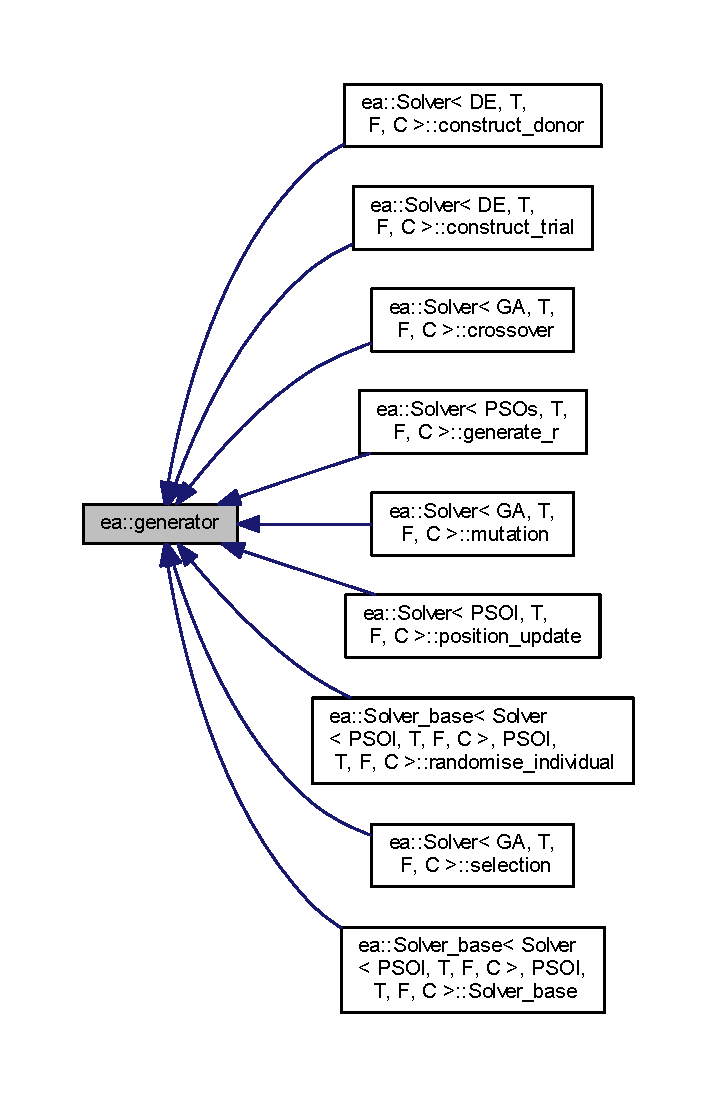
\includegraphics[width=344pt]{namespaceea_a385e8ca8ba4ae2f69dcfffa79f20c2ff_icgraph}
\end{center}
\end{figure}
\mbox{\Hypertarget{namespaceea_a6450b5bf61e9fdca8b6c19267e14c560}\label{namespaceea_a6450b5bf61e9fdca8b6c19267e14c560}} 
\index{ea@{ea}!solve@{solve}}
\index{solve@{solve}!ea@{ea}}
\subsubsection{\texorpdfstring{solve()}{solve()}}
{\footnotesize\ttfamily template$<$typename F , typename C , template$<$ typename $>$ class S, typename T $>$ \\
ea\+::solve (\begin{DoxyParamCaption}\item[{const F \&}]{f,  }\item[{const C \&}]{c,  }\item[{const S$<$ T $>$ \&}]{solver\+\_\+struct,  }\item[{const std\+::string \&}]{problem\+\_\+name }\end{DoxyParamCaption})}



\hyperlink{classea_1_1_solver}{Solver} wrapper function, interface to solvers \+: free function used for benchmarks. 


\begin{DoxyParams}{Parameters}
{\em f} & The objective function \\
\hline
{\em c} & The constraints function \\
\hline
{\em solver\+\_\+struct} & The parameter structure of the solver \\
\hline
{\em problem\+\_\+name} & The name of the problem in std\+::string form. It is used to print results to file. \\
\hline
\end{DoxyParams}
\begin{DoxyReturn}{Returns}
The solution vector 
\end{DoxyReturn}


Definition at line 309 of file ealgorithm\+\_\+base.\+h.



Referenced by bond\+::\+Bond\+Helper$<$ T $>$\+::bond\+\_\+pricing(), bond\+::\+Bond$<$ T $>$\+::compute\+\_\+yield(), and yft\+::\+Interest\+\_\+\+Rate\+\_\+\+Helper$<$ T $>$\+::yieldcurve\+\_\+fitting().


\begin{DoxyCode}
310     \{
311         Solver<S, T, F, C> solver\{ solver\_struct, f, c \};
312         \textcolor{keywordflow}{return} solver.solver\_bench(problem\_name);
313     \}
\end{DoxyCode}
Here is the caller graph for this function\+:
\nopagebreak
\begin{figure}[H]
\begin{center}
\leavevmode
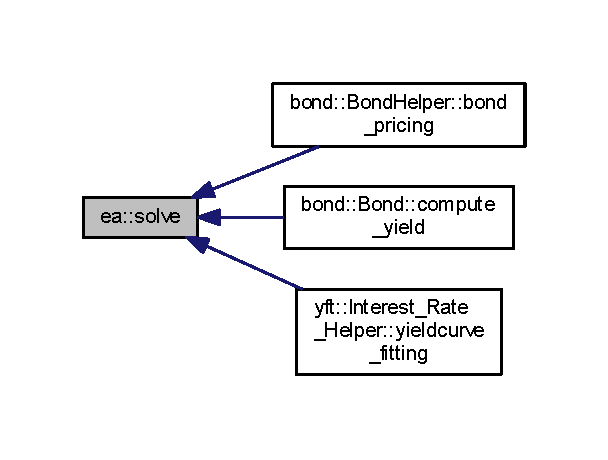
\includegraphics[width=292pt]{namespaceea_a6450b5bf61e9fdca8b6c19267e14c560_icgraph}
\end{center}
\end{figure}


\subsection{Variable Documentation}
\mbox{\Hypertarget{namespaceea_a0a68157259a48341f23eeffca8a1d748}\label{namespaceea_a0a68157259a48341f23eeffca8a1d748}} 
\index{ea@{ea}!inv\+\_\+pi\+\_\+sq@{inv\+\_\+pi\+\_\+sq}}
\index{inv\+\_\+pi\+\_\+sq@{inv\+\_\+pi\+\_\+sq}!ea@{ea}}
\subsubsection{\texorpdfstring{inv\+\_\+pi\+\_\+sq}{inv\_pi\_sq}}
{\footnotesize\ttfamily template$<$typename T $>$ \\
const double ea\+::inv\+\_\+pi\+\_\+sq = 1 / std\+::pow(boost\+::math\+::constants\+::pi$<$T$>$(), 2)}



Inverse square of pi constant. 



Definition at line 307 of file lbestpso.\+h.

\mbox{\Hypertarget{namespaceea_aceb1a704bbda5c44541cd98184c2c224}\label{namespaceea_aceb1a704bbda5c44541cd98184c2c224}} 
\index{ea@{ea}!inv\+\_\+pi\+\_\+sq\+\_\+2@{inv\+\_\+pi\+\_\+sq\+\_\+2}}
\index{inv\+\_\+pi\+\_\+sq\+\_\+2@{inv\+\_\+pi\+\_\+sq\+\_\+2}!ea@{ea}}
\subsubsection{\texorpdfstring{inv\+\_\+pi\+\_\+sq\+\_\+2}{inv\_pi\_sq\_2}}
{\footnotesize\ttfamily template$<$typename T $>$ \\
const double ea\+::inv\+\_\+pi\+\_\+sq\+\_\+2 = 1 / std\+::pow(boost\+::math\+::constants\+::pi$<$T$>$(), 2)}



Inverse square of pi constant. 



Definition at line 331 of file pso\+\_\+sub\+\_\+swarm.\+h.

\mbox{\Hypertarget{namespaceea_a0d4adcfbf42f88a74097673d4564f757}\label{namespaceea_a0d4adcfbf42f88a74097673d4564f757}} 
\index{ea@{ea}!rd@{rd}}
\index{rd@{rd}!ea@{ea}}
\subsubsection{\texorpdfstring{rd}{rd}}
{\footnotesize\ttfamily std\+::random\+\_\+device ea\+::rd}



Random device / Random number generator. 



Definition at line 85 of file ealgorithm\+\_\+base.\+h.


\hypertarget{namespaceirr}{}\section{irr Namespace Reference}
\label{namespaceirr}\index{irr@{irr}}


Internal Rate of Return (I\+RR) namespace.  


\subsection*{Functions}
\begin{DoxyCompactItemize}
\item 
{\footnotesize template$<$typename T $>$ }\\T \hyperlink{namespaceirr_ae00c3409ca39fa2dc47ce61da4169a66}{compute\+\_\+discount\+\_\+factor} (const T \&r, const T \&period, const \hyperlink{namespaceutilities_ad4290e607d0651ce53db6e5c776aca7c}{D\+F\+\_\+type} \&df\+\_\+type)
\begin{DoxyCompactList}\small\item\em Calculates discount factors. \end{DoxyCompactList}\item 
{\footnotesize template$<$typename T $>$ }\\bool \hyperlink{namespaceirr_a6801aa96a307b3f52817dd1a3bcd065e}{constraints\+\_\+irr} (const std\+::vector$<$ T $>$ \&solution, const \hyperlink{namespaceutilities_ab1a1517bf6e62a1acfab5293ca8985c1}{Constraints\+\_\+type} \&constraints\+\_\+type)
\begin{DoxyCompactList}\small\item\em Constraints function for Internal Rate of Return. \end{DoxyCompactList}\item 
{\footnotesize template$<$typename T $>$ }\\T \hyperlink{namespaceirr_ac3411cd2ad174f399c525d8d17dcdad0}{compute\+\_\+pv} (const T \&r, const T \&nominal\+\_\+value, const std\+::vector$<$ T $>$ \&cash\+\_\+flows, const std\+::vector$<$ T $>$ \&time\+\_\+periods, const \hyperlink{namespaceutilities_ad4290e607d0651ce53db6e5c776aca7c}{D\+F\+\_\+type} \&df\+\_\+type)
\begin{DoxyCompactList}\small\item\em Returns the present value of an investment. \end{DoxyCompactList}\item 
{\footnotesize template$<$typename T $>$ }\\T \hyperlink{namespaceirr_abd1d21a84003df6b46dc32c3a30d2269}{penalty\+\_\+irr} (const T \&r)
\begin{DoxyCompactList}\small\item\em Penalty function for I\+RR. \end{DoxyCompactList}\item 
{\footnotesize template$<$typename T $>$ }\\T \hyperlink{namespaceirr_aced01c5e5ef9e171a3b892275d442f8d}{fitness\+\_\+irr} (const std\+::vector$<$ T $>$ \&solution, const T \&price, const T \&nominal\+\_\+value, const std\+::vector$<$ T $>$ \&cash\+\_\+flows, const std\+::vector$<$ T $>$ \&time\+\_\+periods, const \hyperlink{namespaceutilities_ad4290e607d0651ce53db6e5c776aca7c}{D\+F\+\_\+type} \&df\+\_\+type, const bool \&use\+\_\+penalty\+\_\+method)
\begin{DoxyCompactList}\small\item\em This is the fitness function for finding the internal rate of return of a bond, in this case it is equal to its yield to maturity. \end{DoxyCompactList}\end{DoxyCompactItemize}


\subsection{Detailed Description}
Internal Rate of Return (I\+RR) namespace. 

\subsection{Function Documentation}
\mbox{\Hypertarget{namespaceirr_ae00c3409ca39fa2dc47ce61da4169a66}\label{namespaceirr_ae00c3409ca39fa2dc47ce61da4169a66}} 
\index{irr@{irr}!compute\+\_\+discount\+\_\+factor@{compute\+\_\+discount\+\_\+factor}}
\index{compute\+\_\+discount\+\_\+factor@{compute\+\_\+discount\+\_\+factor}!irr@{irr}}
\subsubsection{\texorpdfstring{compute\+\_\+discount\+\_\+factor()}{compute\_discount\_factor()}}
{\footnotesize\ttfamily template$<$typename T $>$ \\
irr\+::compute\+\_\+discount\+\_\+factor (\begin{DoxyParamCaption}\item[{const T \&}]{r,  }\item[{const T \&}]{period,  }\item[{const \hyperlink{namespaceutilities_ad4290e607d0651ce53db6e5c776aca7c}{D\+F\+\_\+type} \&}]{df\+\_\+type }\end{DoxyParamCaption})}



Calculates discount factors. 


\begin{DoxyParams}{Parameters}
{\em r} & Rate \\
\hline
{\em period} & The period the rate was recorded \\
\hline
{\em df\+\_\+type} & The method used to calculate the discount factor \\
\hline
\end{DoxyParams}
\begin{DoxyReturn}{Returns}
The discount factor 
\end{DoxyReturn}


Definition at line 25 of file irr.\+h.



References utilities\+::exp, and utilities\+::frac.



Referenced by bond\+::\+Bond$<$ T $>$\+::compute\+\_\+macaulay\+\_\+duration(), compute\+\_\+pv(), and bond\+::\+Bond\+Helper$<$ T $>$\+::estimate\+\_\+bond\+\_\+pricing().


\begin{DoxyCode}
26     \{
27         \textcolor{keywordflow}{switch} (df\_type)
28         \{
29         \textcolor{keywordflow}{case} (DF\_type::frac): \textcolor{keywordflow}{return} 1 / std::pow((1 + r), period);
30         \textcolor{keywordflow}{case} (DF\_type::exp): \textcolor{keywordflow}{return} std::exp(-r * period);
31             \textcolor{keywordflow}{default}: std::abort();
32         \}
33     \}
\end{DoxyCode}
Here is the caller graph for this function\+:
\nopagebreak
\begin{figure}[H]
\begin{center}
\leavevmode
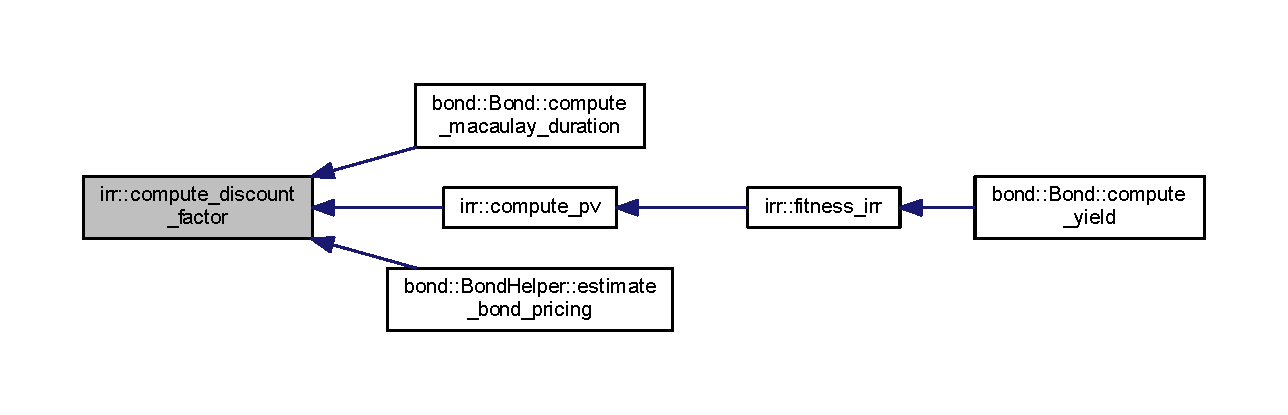
\includegraphics[width=350pt]{namespaceirr_ae00c3409ca39fa2dc47ce61da4169a66_icgraph}
\end{center}
\end{figure}
\mbox{\Hypertarget{namespaceirr_ac3411cd2ad174f399c525d8d17dcdad0}\label{namespaceirr_ac3411cd2ad174f399c525d8d17dcdad0}} 
\index{irr@{irr}!compute\+\_\+pv@{compute\+\_\+pv}}
\index{compute\+\_\+pv@{compute\+\_\+pv}!irr@{irr}}
\subsubsection{\texorpdfstring{compute\+\_\+pv()}{compute\_pv()}}
{\footnotesize\ttfamily template$<$typename T $>$ \\
irr\+::compute\+\_\+pv (\begin{DoxyParamCaption}\item[{const T \&}]{r,  }\item[{const T \&}]{nominal\+\_\+value,  }\item[{const std\+::vector$<$ T $>$ \&}]{cash\+\_\+flows,  }\item[{const std\+::vector$<$ T $>$ \&}]{time\+\_\+periods,  }\item[{const \hyperlink{namespaceutilities_ad4290e607d0651ce53db6e5c776aca7c}{D\+F\+\_\+type} \&}]{df\+\_\+type }\end{DoxyParamCaption})}



Returns the present value of an investment. 


\begin{DoxyParams}{Parameters}
{\em r} & Internal Rate of Return \\
\hline
{\em nominal\+\_\+value} & The nominal value of the investment \\
\hline
{\em cash\+\_\+flows} & The cash flows of the investment \\
\hline
{\em time\+\_\+periods} & The time periods that correspond to the cash flows of the investment \\
\hline
{\em df\+\_\+type} & The method used to calculate the discount factor \\
\hline
\end{DoxyParams}
\begin{DoxyReturn}{Returns}
The present value of the investment 
\end{DoxyReturn}


Definition at line 74 of file irr.\+h.



References compute\+\_\+discount\+\_\+factor().



Referenced by fitness\+\_\+irr().


\begin{DoxyCode}
75     \{
76         assert(cash\_flows.size() == time\_periods.size());
77         \textcolor{keyword}{const} \textcolor{keywordtype}{size\_t}& num\_time\_periods =time\_periods.size();
78         T sum = 0.0;
79         \textcolor{keywordflow}{for} (\textcolor{keywordtype}{size\_t} i = 0; i < num\_time\_periods; ++i)
80         \{
81             sum = sum + cash\_flows[i] * \hyperlink{namespaceirr_ae00c3409ca39fa2dc47ce61da4169a66}{compute\_discount\_factor}(r, time\_periods[i], 
      df\_type);
82         \}
83         \textcolor{keywordflow}{return} sum + nominal\_value * \hyperlink{namespaceirr_ae00c3409ca39fa2dc47ce61da4169a66}{compute\_discount\_factor}(r, time\_periods.back(),
       df\_type);
84     \}
\end{DoxyCode}
Here is the call graph for this function\+:
\nopagebreak
\begin{figure}[H]
\begin{center}
\leavevmode
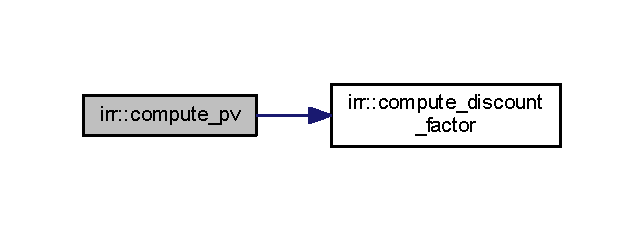
\includegraphics[width=309pt]{namespaceirr_ac3411cd2ad174f399c525d8d17dcdad0_cgraph}
\end{center}
\end{figure}
Here is the caller graph for this function\+:
\nopagebreak
\begin{figure}[H]
\begin{center}
\leavevmode
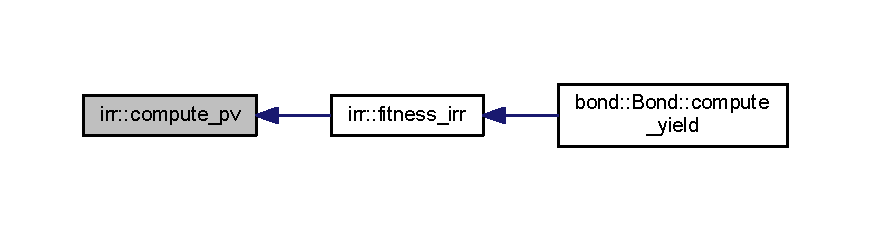
\includegraphics[width=350pt]{namespaceirr_ac3411cd2ad174f399c525d8d17dcdad0_icgraph}
\end{center}
\end{figure}
\mbox{\Hypertarget{namespaceirr_a6801aa96a307b3f52817dd1a3bcd065e}\label{namespaceirr_a6801aa96a307b3f52817dd1a3bcd065e}} 
\index{irr@{irr}!constraints\+\_\+irr@{constraints\+\_\+irr}}
\index{constraints\+\_\+irr@{constraints\+\_\+irr}!irr@{irr}}
\subsubsection{\texorpdfstring{constraints\+\_\+irr()}{constraints\_irr()}}
{\footnotesize\ttfamily template$<$typename T $>$ \\
irr\+::constraints\+\_\+irr (\begin{DoxyParamCaption}\item[{const std\+::vector$<$ T $>$ \&}]{solution,  }\item[{const \hyperlink{namespaceutilities_ab1a1517bf6e62a1acfab5293ca8985c1}{Constraints\+\_\+type} \&}]{constraints\+\_\+type }\end{DoxyParamCaption})}



Constraints function for Internal Rate of Return. 


\begin{DoxyParams}{Parameters}
{\em solution} & Internal Rate of Return candindate solution \\
\hline
{\em constraints\+\_\+type} & Type of constraints used \\
\hline
\end{DoxyParams}
\begin{DoxyReturn}{Returns}
True if constraints are satisfied, false otherwise 
\end{DoxyReturn}


Definition at line 42 of file irr.\+h.



References utilities\+::none, utilities\+::normal, and utilities\+::tight.



Referenced by bond\+::\+Bond$<$ T $>$\+::compute\+\_\+yield().


\begin{DoxyCode}
43     \{
44         \textcolor{keywordflow}{switch} (constraints\_type)
45         \{
46         \textcolor{keywordflow}{case}(Constraints\_type::normal):
47         \{
48             \textcolor{keyword}{const} T& r = solution[0];
49             \textcolor{keywordflow}{if} (r > 0 && r < 1)
50             \{
51                 \textcolor{keywordflow}{return} \textcolor{keyword}{true};
52             \}
53             \textcolor{keywordflow}{else}
54             \{
55                 \textcolor{keywordflow}{return} \textcolor{keyword}{false};
56             \}
57         \}
58         \textcolor{keywordflow}{case}(Constraints\_type::tight): \textcolor{keywordflow}{return} \textcolor{keyword}{true};
59         \textcolor{keywordflow}{case}(Constraints\_type::none): \textcolor{keywordflow}{return} \textcolor{keyword}{true};
60             \textcolor{keywordflow}{default}: std::abort();
61         \}
62     \}
\end{DoxyCode}
Here is the caller graph for this function\+:
\nopagebreak
\begin{figure}[H]
\begin{center}
\leavevmode
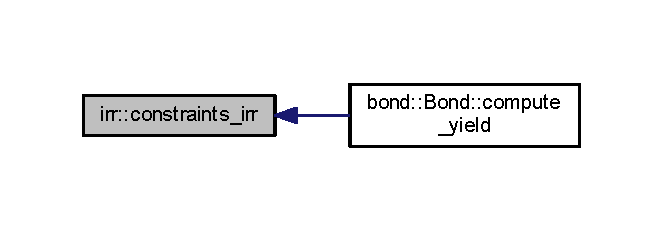
\includegraphics[width=318pt]{namespaceirr_a6801aa96a307b3f52817dd1a3bcd065e_icgraph}
\end{center}
\end{figure}
\mbox{\Hypertarget{namespaceirr_aced01c5e5ef9e171a3b892275d442f8d}\label{namespaceirr_aced01c5e5ef9e171a3b892275d442f8d}} 
\index{irr@{irr}!fitness\+\_\+irr@{fitness\+\_\+irr}}
\index{fitness\+\_\+irr@{fitness\+\_\+irr}!irr@{irr}}
\subsubsection{\texorpdfstring{fitness\+\_\+irr()}{fitness\_irr()}}
{\footnotesize\ttfamily template$<$typename T $>$ \\
irr\+::fitness\+\_\+irr (\begin{DoxyParamCaption}\item[{const std\+::vector$<$ T $>$ \&}]{solution,  }\item[{const T \&}]{price,  }\item[{const T \&}]{nominal\+\_\+value,  }\item[{const std\+::vector$<$ T $>$ \&}]{cash\+\_\+flows,  }\item[{const std\+::vector$<$ T $>$ \&}]{time\+\_\+periods,  }\item[{const \hyperlink{namespaceutilities_ad4290e607d0651ce53db6e5c776aca7c}{D\+F\+\_\+type} \&}]{df\+\_\+type,  }\item[{const bool \&}]{use\+\_\+penalty\+\_\+method }\end{DoxyParamCaption})}



This is the fitness function for finding the internal rate of return of a bond, in this case it is equal to its yield to maturity. 


\begin{DoxyParams}{Parameters}
{\em solution} & Internal Rate of Return candindate solution \\
\hline
{\em price} & The present value of the investment \\
\hline
{\em nominal\+\_\+value} & The nominal value of the investment \\
\hline
{\em cash\+\_\+flows} & The cash flows of the investment \\
\hline
{\em time\+\_\+periods} & The time periods that correspond to the cash flows of the investment \\
\hline
{\em df\+\_\+type} & The method used to calculate the discount factor \\
\hline
{\em use\+\_\+penalty\+\_\+method} & Whether to use the penalty method defined for I\+RR or not \\
\hline
\end{DoxyParams}
\begin{DoxyReturn}{Returns}
The fitness cost of I\+RR 
\end{DoxyReturn}


Definition at line 116 of file irr.\+h.



References compute\+\_\+pv(), and penalty\+\_\+irr().



Referenced by bond\+::\+Bond$<$ T $>$\+::compute\+\_\+yield().


\begin{DoxyCode}
118     \{
119         T sum\_of\_squares = 0;
120         sum\_of\_squares = sum\_of\_squares + std::pow(price - \hyperlink{namespaceirr_ac3411cd2ad174f399c525d8d17dcdad0}{compute\_pv}(solution[0], nominal\_value,
       cash\_flows, time\_periods, df\_type), 2);
121         \textcolor{keywordflow}{if} (use\_penalty\_method)
122         \{
123             \textcolor{keywordflow}{return} sum\_of\_squares + \hyperlink{namespaceirr_abd1d21a84003df6b46dc32c3a30d2269}{penalty\_irr}(solution[0]);
124         \}
125         \textcolor{keywordflow}{else}
126         \{
127             \textcolor{keywordflow}{return} sum\_of\_squares;
128         \}
129     \}
\end{DoxyCode}
Here is the call graph for this function\+:
\nopagebreak
\begin{figure}[H]
\begin{center}
\leavevmode
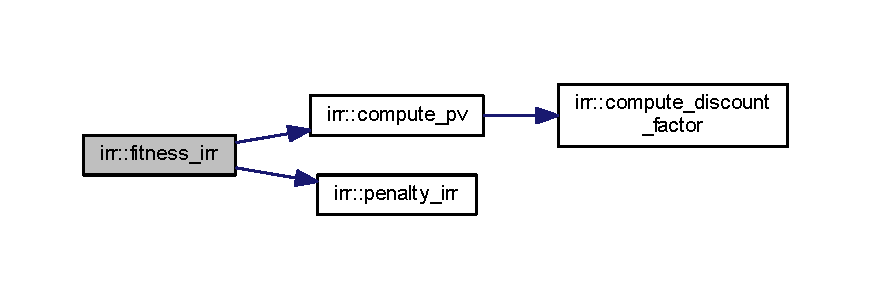
\includegraphics[width=350pt]{namespaceirr_aced01c5e5ef9e171a3b892275d442f8d_cgraph}
\end{center}
\end{figure}
Here is the caller graph for this function\+:
\nopagebreak
\begin{figure}[H]
\begin{center}
\leavevmode
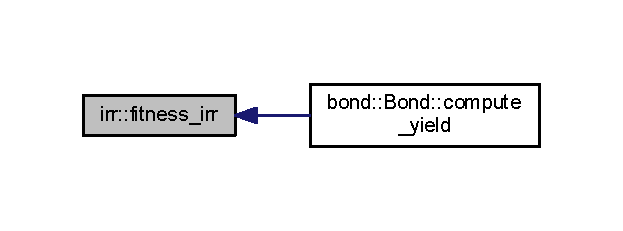
\includegraphics[width=299pt]{namespaceirr_aced01c5e5ef9e171a3b892275d442f8d_icgraph}
\end{center}
\end{figure}
\mbox{\Hypertarget{namespaceirr_abd1d21a84003df6b46dc32c3a30d2269}\label{namespaceirr_abd1d21a84003df6b46dc32c3a30d2269}} 
\index{irr@{irr}!penalty\+\_\+irr@{penalty\+\_\+irr}}
\index{penalty\+\_\+irr@{penalty\+\_\+irr}!irr@{irr}}
\subsubsection{\texorpdfstring{penalty\+\_\+irr()}{penalty\_irr()}}
{\footnotesize\ttfamily template$<$typename T $>$ \\
irr\+::penalty\+\_\+irr (\begin{DoxyParamCaption}\item[{const T \&}]{r }\end{DoxyParamCaption})}



Penalty function for I\+RR. 


\begin{DoxyParams}{Parameters}
{\em r} & Candidate solution for the Internal Rate of Return \\
\hline
\end{DoxyParams}
\begin{DoxyReturn}{Returns}
A penalty value, if constraints are not satisfied 
\end{DoxyReturn}


Definition at line 92 of file irr.\+h.



Referenced by fitness\+\_\+irr().


\begin{DoxyCode}
93     \{
94         T sum = 0;
95         \textcolor{keyword}{const} T C = 1000;
96         \textcolor{keywordflow}{if} (r < 0 || r > 1)
97         \{
98             sum = sum + C * std::pow(std::abs(r), 2);
99         \}
100         \textcolor{keywordflow}{return} sum;
101     \}
\end{DoxyCode}
Here is the caller graph for this function\+:
\nopagebreak
\begin{figure}[H]
\begin{center}
\leavevmode
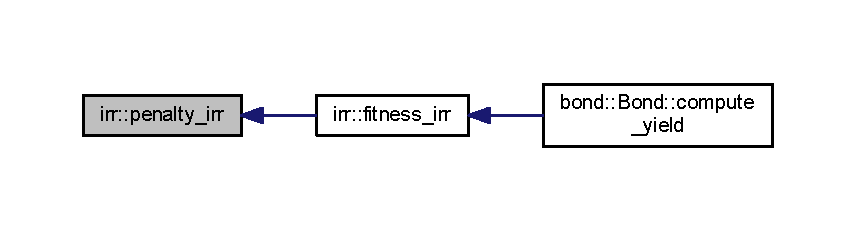
\includegraphics[width=350pt]{namespaceirr_abd1d21a84003df6b46dc32c3a30d2269_icgraph}
\end{center}
\end{figure}

\hypertarget{namespacenss}{}\section{nss Namespace Reference}
\label{namespacenss}\index{nss@{nss}}


Nelson-\/\+Siegel-\/\+Svensson (N\+SS) model namespace.  


\subsection*{Functions}
\begin{DoxyCompactItemize}
\item 
{\footnotesize template$<$typename T $>$ }\\bool \hyperlink{namespacenss_a39de3569a71e773f9da82c713eb7e6eb}{constraints\+\_\+svensson} (const std\+::vector$<$ T $>$ \&solution, const Constraints\+\_\+type \&constraints\+\_\+type)
\begin{DoxyCompactList}\small\item\em Constraints function for the N\+SS model. \end{DoxyCompactList}\item 
{\footnotesize template$<$typename T $>$ }\\T \hyperlink{namespacenss_a71aad246261afa16f8bb1a4057570d4b}{svensson} (const std\+::vector$<$ T $>$ \&solution, const T \&m)
\begin{DoxyCompactList}\small\item\em Spot interest rate at term m using the N\+SS model. \end{DoxyCompactList}\item 
{\footnotesize template$<$typename T $>$ }\\T \hyperlink{namespacenss_a009a0ebbca20f7969d0c2ed5a241aa82}{penalty\+\_\+svensson} (const std\+::vector$<$ T $>$ \&solution)
\begin{DoxyCompactList}\small\item\em Penalty function for N\+SS. \end{DoxyCompactList}\end{DoxyCompactItemize}


\subsection{Detailed Description}
Nelson-\/\+Siegel-\/\+Svensson (N\+SS) model namespace. 

\subsection{Function Documentation}
\mbox{\Hypertarget{namespacenss_a39de3569a71e773f9da82c713eb7e6eb}\label{namespacenss_a39de3569a71e773f9da82c713eb7e6eb}} 
\index{nss@{nss}!constraints\+\_\+svensson@{constraints\+\_\+svensson}}
\index{constraints\+\_\+svensson@{constraints\+\_\+svensson}!nss@{nss}}
\subsubsection{\texorpdfstring{constraints\+\_\+svensson()}{constraints\_svensson()}}
{\footnotesize\ttfamily template$<$typename T $>$ \\
nss\+::constraints\+\_\+svensson (\begin{DoxyParamCaption}\item[{const std\+::vector$<$ T $>$ \&}]{solution,  }\item[{const Constraints\+\_\+type \&}]{constraints\+\_\+type }\end{DoxyParamCaption})}



Constraints function for the N\+SS model. 


\begin{DoxyParams}{Parameters}
{\em solution} & N\+SS parameters candindate solution \\
\hline
{\em constraints\+\_\+type} & Type of constraints used \\
\hline
\end{DoxyParams}
\begin{DoxyReturn}{Returns}
True if constraints are satisfied, false otherwise 
\end{DoxyReturn}


Definition at line 18 of file svensson.\+h.



Referenced by bond\+::\+Bond\+Helper$<$ T $>$\+::bond\+\_\+pricing(), and yft\+::\+Interest\+\_\+\+Rate\+\_\+\+Helper$<$ T $>$\+::yieldcurve\+\_\+fitting().


\begin{DoxyCode}
19     \{
20         \textcolor{keywordflow}{switch} (constraints\_type)
21         \{
22         \textcolor{keywordflow}{case}(Constraints\_type::normal):
23         \{
24             \textcolor{keyword}{const} T& b0 = solution[0];
25             \textcolor{keyword}{const} T& b1 = solution[1];
26             \textcolor{keyword}{const} T& tau1 = solution[4];
27             \textcolor{keyword}{const} T& tau2 = solution[5];
28             \textcolor{keywordflow}{if} (b0 > 0 && b0 + b1 > 0 && tau1 > 0 && tau2 > 0)
29             \{
30                 \textcolor{keywordflow}{return} \textcolor{keyword}{true};
31             \}
32             \textcolor{keywordflow}{else}
33             \{
34                 \textcolor{keywordflow}{return} \textcolor{keyword}{false};
35             \}
36         \}
37         \textcolor{keywordflow}{case}(Constraints\_type::tight):
38         \{
39             \textcolor{keyword}{const} T& b0 = solution[0];
40             \textcolor{keyword}{const} T& b1 = solution[1];
41             \textcolor{keyword}{const} T& b2 = solution[2];
42             \textcolor{keyword}{const} T& b3 = solution[3];
43             \textcolor{keyword}{const} T& tau1 = solution[4];
44             \textcolor{keyword}{const} T& tau2 = solution[5];
45             \textcolor{keywordflow}{if} ((b0 > 0 && b0 < 15)
46                 && (b1 > -15 && b1 < 30)
47                 && (b2 > -30 && b2 < 30)
48                 && (b3 > -30 && b3 < 30)
49                 && (tau1 > 0 && tau1 < 2.5)
50                 && (tau2 > 2.5 && tau2 < 5.5))
51             \{
52                 \textcolor{keywordflow}{return} \textcolor{keyword}{true};
53             \}
54             \textcolor{keywordflow}{else}
55             \{
56                 \textcolor{keywordflow}{return} \textcolor{keyword}{false};
57             \}
58         \}
59         \textcolor{keywordflow}{case}(Constraints\_type::none): \textcolor{keywordflow}{return} \textcolor{keyword}{true};
60         \textcolor{keywordflow}{default}: std::abort();
61         \}
62     \}
\end{DoxyCode}
Here is the caller graph for this function\+:
\nopagebreak
\begin{figure}[H]
\begin{center}
\leavevmode
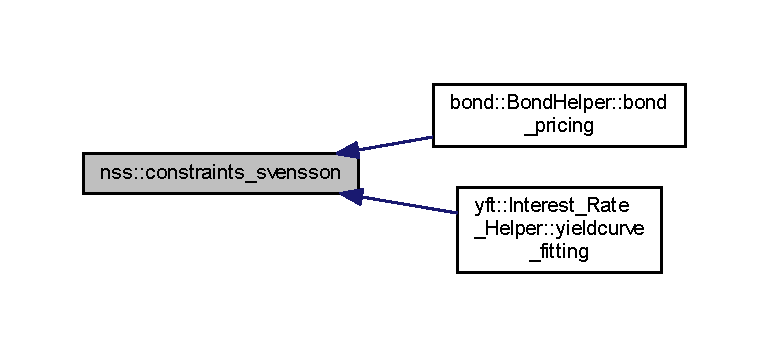
\includegraphics[width=350pt]{namespacenss_a39de3569a71e773f9da82c713eb7e6eb_icgraph}
\end{center}
\end{figure}
\mbox{\Hypertarget{namespacenss_a009a0ebbca20f7969d0c2ed5a241aa82}\label{namespacenss_a009a0ebbca20f7969d0c2ed5a241aa82}} 
\index{nss@{nss}!penalty\+\_\+svensson@{penalty\+\_\+svensson}}
\index{penalty\+\_\+svensson@{penalty\+\_\+svensson}!nss@{nss}}
\subsubsection{\texorpdfstring{penalty\+\_\+svensson()}{penalty\_svensson()}}
{\footnotesize\ttfamily template$<$typename T $>$ \\
nss\+::penalty\+\_\+svensson (\begin{DoxyParamCaption}\item[{const std\+::vector$<$ T $>$ \&}]{solution }\end{DoxyParamCaption})}



Penalty function for N\+SS. 


\begin{DoxyParams}{Parameters}
{\em solution} & Candidate solution for the parameters of N\+SS \\
\hline
\end{DoxyParams}
\begin{DoxyReturn}{Returns}
A penalty value, if constraints are not satisfied 
\end{DoxyReturn}


Definition at line 99 of file svensson.\+h.



Referenced by bond\+::\+Bond\+Helper$<$ T $>$\+::fitness\+\_\+bond\+\_\+pricing\+\_\+prices(), bond\+::\+Bond\+Helper$<$ T $>$\+::fitness\+\_\+bond\+\_\+pricing\+\_\+yields(), and yft\+::\+Interest\+\_\+\+Rate\+\_\+\+Helper$<$ T $>$\+::fitness\+\_\+yield\+\_\+curve\+\_\+fitting().


\begin{DoxyCode}
100     \{
101         T sum = 0;
102         \textcolor{keyword}{const} T& b0 = solution[0];
103         \textcolor{keyword}{const} T& b1 = solution[1];
104         \textcolor{keyword}{const} T& b2 = solution[2];
105         \textcolor{keyword}{const} T& b3 = solution[3];
106         \textcolor{keyword}{const} T& tau1 = solution[4];
107         \textcolor{keyword}{const} T& tau2 = solution[5];
108         \textcolor{keyword}{const} T C = 100000;
109         \textcolor{keywordflow}{if} (b0 < 0 || b0 > 15)
110         \{
111             sum = sum + C * std::pow(std::abs(b0), 2);
112         \}
113         \textcolor{keywordflow}{if} (b0 + b1 < 0)
114         \{
115             sum = sum + C * std::pow(std::abs(b0 + b1), 2);
116         \}
117         \textcolor{keywordflow}{if} (b1 < -15 || b1 > 30)
118         \{
119             sum = sum + C * std::pow(std::abs(b1), 2);
120         \}
121         \textcolor{keywordflow}{if} (b2 < -30 || b2 > 30)
122         \{
123             sum = sum + C * std::pow(std::abs(b1), 2);
124         \}
125         \textcolor{keywordflow}{if} (b3 < -30 || b3 > 30)
126         \{
127             sum = sum + C * std::pow(std::abs(b1), 2);
128         \}
129         \textcolor{keywordflow}{if} (tau1 < 0 || tau1 > 2.5)
130         \{
131             sum = sum + C * std::pow(std::abs(tau2), 2);
132         \}
133         \textcolor{keywordflow}{if} (tau2 < 2.5 || tau2 > 5.5)
134         \{
135             sum = sum + C * std::pow(std::abs(tau2), 2);
136         \}
137         \textcolor{keywordflow}{return} sum;
138     \}
\end{DoxyCode}
Here is the caller graph for this function\+:
\nopagebreak
\begin{figure}[H]
\begin{center}
\leavevmode
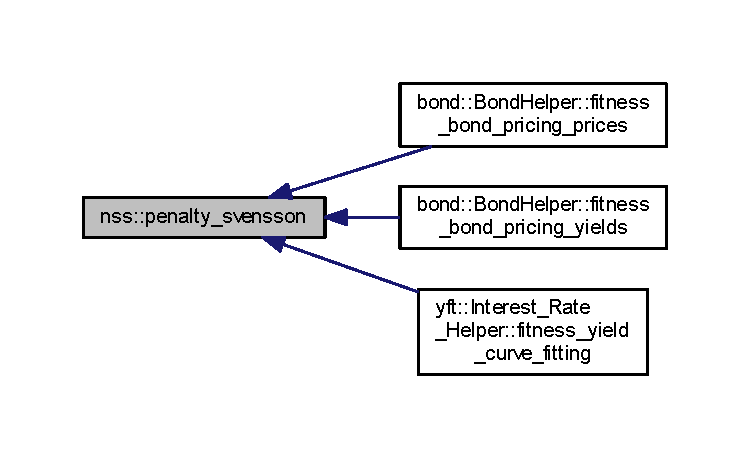
\includegraphics[width=350pt]{namespacenss_a009a0ebbca20f7969d0c2ed5a241aa82_icgraph}
\end{center}
\end{figure}
\mbox{\Hypertarget{namespacenss_a71aad246261afa16f8bb1a4057570d4b}\label{namespacenss_a71aad246261afa16f8bb1a4057570d4b}} 
\index{nss@{nss}!svensson@{svensson}}
\index{svensson@{svensson}!nss@{nss}}
\subsubsection{\texorpdfstring{svensson()}{svensson()}}
{\footnotesize\ttfamily template$<$typename T $>$ \\
nss\+::svensson (\begin{DoxyParamCaption}\item[{const std\+::vector$<$ T $>$ \&}]{solution,  }\item[{const T \&}]{m }\end{DoxyParamCaption})}



Spot interest rate at term m using the N\+SS model. 


\begin{DoxyParams}{Parameters}
{\em solution} & Candidate solution for the parameters of N\+SS \\
\hline
{\em m} & The term at which the spot interest rate is recorded \\
\hline
\end{DoxyParams}
\begin{DoxyReturn}{Returns}
The spot interest rate at term m 
\end{DoxyReturn}


Definition at line 71 of file svensson.\+h.



Referenced by bond\+::\+Bond\+Helper$<$ T $>$\+::estimate\+\_\+bond\+\_\+pricing(), yft\+::\+Interest\+\_\+\+Rate\+\_\+\+Helper$<$ T $>$\+::fitness\+\_\+yield\+\_\+curve\+\_\+fitting(), and yft\+::\+Interest\+\_\+\+Rate\+\_\+\+Helper$<$ T $>$\+::yieldcurve\+\_\+fitting().


\begin{DoxyCode}
72     \{
73         \textcolor{keyword}{const} T& b0 = solution[0];
74         \textcolor{keyword}{const} T& b1 = solution[1];
75         \textcolor{keyword}{const} T& b2 = solution[2];
76         \textcolor{keyword}{const} T& b3 = solution[3];
77         \textcolor{keyword}{const} T& tau1 = solution[4];
78         \textcolor{keyword}{const} T& tau2 = solution[5];
79         \textcolor{keywordflow}{if} (m == 0)
80         \{
81             \textcolor{keywordflow}{return} b0 + b1;
82         \}
83         \textcolor{keywordflow}{else}
84         \{
85             T result = b0;
86             result = result + b1 * ((1 - (std::exp(-m / tau1))) / (m / tau1));
87             result = result + b2 * (((1 - (std::exp(-m / tau1))) / (m / tau1)) - std::exp(-m / tau1));
88             result = result + b3 * (((1 - (std::exp(-m / tau2))) / (m / tau2)) - std::exp(-m / tau2));
89             \textcolor{keywordflow}{return} result;
90         \}
91     \}
\end{DoxyCode}
Here is the caller graph for this function\+:
\nopagebreak
\begin{figure}[H]
\begin{center}
\leavevmode
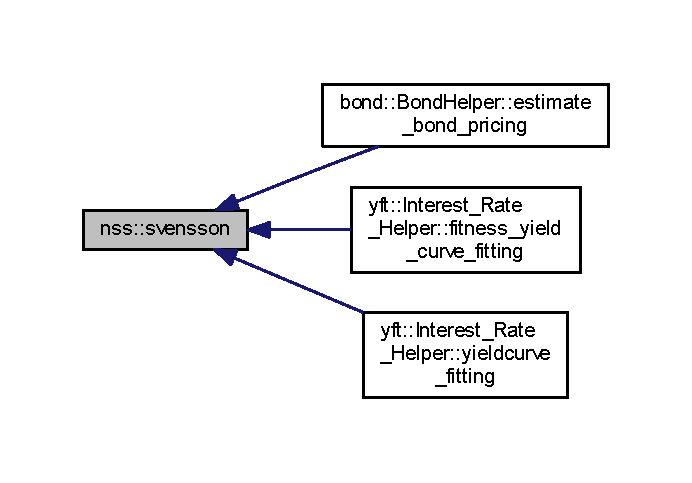
\includegraphics[width=332pt]{namespacenss_a71aad246261afa16f8bb1a4057570d4b_icgraph}
\end{center}
\end{figure}

\hypertarget{namespaceutilities}{}\section{utilities Namespace Reference}
\label{namespaceutilities}\index{utilities@{utilities}}


Utilities namespace.  


\subsection*{Enumerations}
\begin{DoxyCompactItemize}
\item 
enum \hyperlink{namespaceutilities_ad4290e607d0651ce53db6e5c776aca7c}{D\+F\+\_\+type} \{ \hyperlink{namespaceutilities_ad4290e607d0651ce53db6e5c776aca7ca8a3baba97ec51277ed8ac64e456f6027}{D\+F\+\_\+type\+::frac}, 
\hyperlink{namespaceutilities_ad4290e607d0651ce53db6e5c776aca7cab0ab0254bd58eb87eaee3172ba49fefb}{D\+F\+\_\+type\+::exp}
 \}\begin{DoxyCompactList}\small\item\em Enumeration for discount factor types/methods. \end{DoxyCompactList}
\item 
enum \hyperlink{namespaceutilities_ab1a1517bf6e62a1acfab5293ca8985c1}{Constraints\+\_\+type} \{ \hyperlink{namespaceutilities_ab1a1517bf6e62a1acfab5293ca8985c1afea087517c26fadd409bd4b9dc642555}{Constraints\+\_\+type\+::normal}, 
\hyperlink{namespaceutilities_ab1a1517bf6e62a1acfab5293ca8985c1a0423fa423baf1ea8139f6662869faf2f}{Constraints\+\_\+type\+::tight}, 
\hyperlink{namespaceutilities_ab1a1517bf6e62a1acfab5293ca8985c1a334c4a4c42fdb79d7ebc3e73b517e6f8}{Constraints\+\_\+type\+::none}
 \}\begin{DoxyCompactList}\small\item\em Enumeration for types of constraints for the optimisation problems. \end{DoxyCompactList}
\end{DoxyCompactItemize}
\subsection*{Functions}
\begin{DoxyCompactItemize}
\item 
{\footnotesize template$<$typename T $>$ }\\std\+::ostream \& \hyperlink{namespaceutilities_a4b168c00efe29cabc5846b48225a6e52}{operator$<$$<$} (std\+::ostream \&stream, const std\+::vector$<$ T $>$ \&vector)
\begin{DoxyCompactList}\small\item\em Overload the operator $<$$<$ for printing vectors. \end{DoxyCompactList}\end{DoxyCompactItemize}


\subsection{Detailed Description}
Utilities namespace. 

\subsection{Enumeration Type Documentation}
\mbox{\Hypertarget{namespaceutilities_ab1a1517bf6e62a1acfab5293ca8985c1}\label{namespaceutilities_ab1a1517bf6e62a1acfab5293ca8985c1}} 
\index{utilities@{utilities}!Constraints\+\_\+type@{Constraints\+\_\+type}}
\index{Constraints\+\_\+type@{Constraints\+\_\+type}!utilities@{utilities}}
\subsubsection{\texorpdfstring{Constraints\+\_\+type}{Constraints\_type}}
{\footnotesize\ttfamily enum \hyperlink{namespaceutilities_ab1a1517bf6e62a1acfab5293ca8985c1}{utilities\+::\+Constraints\+\_\+type}\hspace{0.3cm}{\ttfamily [strong]}}



Enumeration for types of constraints for the optimisation problems. 

\begin{DoxyEnumFields}{Enumerator}
\raisebox{\heightof{T}}[0pt][0pt]{\index{normal@{normal}!utilities@{utilities}}\index{utilities@{utilities}!normal@{normal}}}\mbox{\Hypertarget{namespaceutilities_ab1a1517bf6e62a1acfab5293ca8985c1afea087517c26fadd409bd4b9dc642555}\label{namespaceutilities_ab1a1517bf6e62a1acfab5293ca8985c1afea087517c26fadd409bd4b9dc642555}} 
normal&Use the normal constraints \\
\hline

\raisebox{\heightof{T}}[0pt][0pt]{\index{tight@{tight}!utilities@{utilities}}\index{utilities@{utilities}!tight@{tight}}}\mbox{\Hypertarget{namespaceutilities_ab1a1517bf6e62a1acfab5293ca8985c1a0423fa423baf1ea8139f6662869faf2f}\label{namespaceutilities_ab1a1517bf6e62a1acfab5293ca8985c1a0423fa423baf1ea8139f6662869faf2f}} 
tight&Use tighter constraints \\
\hline

\raisebox{\heightof{T}}[0pt][0pt]{\index{none@{none}!utilities@{utilities}}\index{utilities@{utilities}!none@{none}}}\mbox{\Hypertarget{namespaceutilities_ab1a1517bf6e62a1acfab5293ca8985c1a334c4a4c42fdb79d7ebc3e73b517e6f8}\label{namespaceutilities_ab1a1517bf6e62a1acfab5293ca8985c1a334c4a4c42fdb79d7ebc3e73b517e6f8}} 
none&Ignore constraints \\
\hline

\end{DoxyEnumFields}


Definition at line 25 of file utilities.\+h.


\begin{DoxyCode}
26     \{ 
27         \hyperlink{namespaceutilities_ab1a1517bf6e62a1acfab5293ca8985c1afea087517c26fadd409bd4b9dc642555}{normal}, 
28         \hyperlink{namespaceutilities_ab1a1517bf6e62a1acfab5293ca8985c1a0423fa423baf1ea8139f6662869faf2f}{tight}, 
29         \hyperlink{namespaceea_a8e369877773b4db67b8512efdb4f8f89a334c4a4c42fdb79d7ebc3e73b517e6f8}{none} 
30     \};
\end{DoxyCode}
\mbox{\Hypertarget{namespaceutilities_ad4290e607d0651ce53db6e5c776aca7c}\label{namespaceutilities_ad4290e607d0651ce53db6e5c776aca7c}} 
\index{utilities@{utilities}!D\+F\+\_\+type@{D\+F\+\_\+type}}
\index{D\+F\+\_\+type@{D\+F\+\_\+type}!utilities@{utilities}}
\subsubsection{\texorpdfstring{D\+F\+\_\+type}{DF\_type}}
{\footnotesize\ttfamily enum \hyperlink{namespaceutilities_ad4290e607d0651ce53db6e5c776aca7c}{utilities\+::\+D\+F\+\_\+type}\hspace{0.3cm}{\ttfamily [strong]}}



Enumeration for discount factor types/methods. 

\begin{DoxyEnumFields}{Enumerator}
\raisebox{\heightof{T}}[0pt][0pt]{\index{frac@{frac}!utilities@{utilities}}\index{utilities@{utilities}!frac@{frac}}}\mbox{\Hypertarget{namespaceutilities_ad4290e607d0651ce53db6e5c776aca7ca8a3baba97ec51277ed8ac64e456f6027}\label{namespaceutilities_ad4290e607d0651ce53db6e5c776aca7ca8a3baba97ec51277ed8ac64e456f6027}} 
frac&Use fractional form to calculate the discount factor \\
\hline

\raisebox{\heightof{T}}[0pt][0pt]{\index{exp@{exp}!utilities@{utilities}}\index{utilities@{utilities}!exp@{exp}}}\mbox{\Hypertarget{namespaceutilities_ad4290e607d0651ce53db6e5c776aca7cab0ab0254bd58eb87eaee3172ba49fefb}\label{namespaceutilities_ad4290e607d0651ce53db6e5c776aca7cab0ab0254bd58eb87eaee3172ba49fefb}} 
exp&Use the exponential form to calculate the discount factor \\
\hline

\end{DoxyEnumFields}


Definition at line 17 of file utilities.\+h.


\begin{DoxyCode}
18     \{
19         \hyperlink{namespaceutilities_ad4290e607d0651ce53db6e5c776aca7ca8a3baba97ec51277ed8ac64e456f6027}{frac}, 
20         \hyperlink{namespaceutilities_ad4290e607d0651ce53db6e5c776aca7cab0ab0254bd58eb87eaee3172ba49fefb}{exp} 
21     \};
\end{DoxyCode}


\subsection{Function Documentation}
\mbox{\Hypertarget{namespaceutilities_a4b168c00efe29cabc5846b48225a6e52}\label{namespaceutilities_a4b168c00efe29cabc5846b48225a6e52}} 
\index{utilities@{utilities}!operator$<$$<$@{operator$<$$<$}}
\index{operator$<$$<$@{operator$<$$<$}!utilities@{utilities}}
\subsubsection{\texorpdfstring{operator$<$$<$()}{operator<<()}}
{\footnotesize\ttfamily template$<$typename T $>$ \\
utilities\+::operator$<$$<$ (\begin{DoxyParamCaption}\item[{std\+::ostream \&}]{stream,  }\item[{const std\+::vector$<$ T $>$ \&}]{vector }\end{DoxyParamCaption})}



Overload the operator $<$$<$ for printing vectors. 


\begin{DoxyParams}{Parameters}
{\em stream} & An out stream \\
\hline
{\em vector} & A vector \\
\hline
\end{DoxyParams}
\begin{DoxyReturn}{Returns}
An out stream of the vector in the form \mbox{[}...\mbox{]} 
\end{DoxyReturn}


Definition at line 38 of file utilities.\+h.


\begin{DoxyCode}
39     \{
40         \textcolor{keywordflow}{if} (!vector.empty())
41         \{
42             stream << \textcolor{stringliteral}{"[ "};
43             std::copy(vector.begin(), vector.end(), std::ostream\_iterator<T>(stream, \textcolor{stringliteral}{" "}));
44             stream << \textcolor{stringliteral}{"]"};
45         \}
46         \textcolor{keywordflow}{return} stream;
47     \}
\end{DoxyCode}

\hypertarget{namespaceyft}{}\section{yft Namespace Reference}
\label{namespaceyft}\index{yft@{yft}}


Yield Curve Fitting namespace.  


\subsection*{Classes}
\begin{DoxyCompactItemize}
\item 
struct \hyperlink{structyft_1_1_interest___rate}{Interest\+\_\+\+Rate}
\begin{DoxyCompactList}\small\item\em Structure for interest rates. \end{DoxyCompactList}\item 
class \hyperlink{classyft_1_1_interest___rate___helper}{Interest\+\_\+\+Rate\+\_\+\+Helper}
\begin{DoxyCompactList}\small\item\em A class for the yield-\/curve-\/fitting problem. \end{DoxyCompactList}\end{DoxyCompactItemize}
\subsection*{Functions}
\begin{DoxyCompactItemize}
\item 
{\footnotesize template$<$typename T $>$ }\\std\+::vector$<$ \hyperlink{structyft_1_1_interest___rate}{Interest\+\_\+\+Rate}$<$ T $>$ $>$ \hyperlink{namespaceyft_a5e004e321696f199f8cf25b1dc604108}{read\+\_\+ir\+\_\+from\+\_\+file} (const std\+::string \&filename)
\begin{DoxyCompactList}\small\item\em Reads the interest rates and periods from file and constructs a vector of interest rate structs. \end{DoxyCompactList}\end{DoxyCompactItemize}


\subsection{Detailed Description}
Yield Curve Fitting namespace. 

\subsection{Function Documentation}
\mbox{\Hypertarget{namespaceyft_a5e004e321696f199f8cf25b1dc604108}\label{namespaceyft_a5e004e321696f199f8cf25b1dc604108}} 
\index{yft@{yft}!read\+\_\+ir\+\_\+from\+\_\+file@{read\+\_\+ir\+\_\+from\+\_\+file}}
\index{read\+\_\+ir\+\_\+from\+\_\+file@{read\+\_\+ir\+\_\+from\+\_\+file}!yft@{yft}}
\subsubsection{\texorpdfstring{read\+\_\+ir\+\_\+from\+\_\+file()}{read\_ir\_from\_file()}}
{\footnotesize\ttfamily template$<$typename T $>$ \\
yft\+::read\+\_\+ir\+\_\+from\+\_\+file (\begin{DoxyParamCaption}\item[{const std\+::string \&}]{filename }\end{DoxyParamCaption})}



Reads the interest rates and periods from file and constructs a vector of interest rate structs. 


\begin{DoxyParams}{Parameters}
{\em filename} & The name of the input file as an std\+::string \\
\hline
\end{DoxyParams}
\begin{DoxyReturn}{Returns}
A vector of \hyperlink{structyft_1_1_interest___rate}{Interest\+\_\+\+Rate} objects 
\end{DoxyReturn}


Definition at line 45 of file yield\+\_\+curve\+\_\+fitting.\+h.


\begin{DoxyCode}
46     \{
47         std::vector<Interest\_Rate<T>> ir\_vec;
48         std::ifstream input(filename);
49         \textcolor{keywordflow}{for} (std::string line; getline(input, line); )
50         \{
51             T period;
52             T rate;
53             std::istringstream stream(line);
54             stream >> period >> rate;
55             \textcolor{keyword}{const} Interest\_Rate<T> ir\{ period, rate \};
56             ir\_vec.push\_back(ir);
57         \}
58         \textcolor{keywordflow}{return} ir\_vec;
59     \}
\end{DoxyCode}

\chapter{Class Documentation}
\hypertarget{classbond_1_1_bond}{}\section{bond\+:\+:Bond$<$ T $>$ Class Template Reference}
\label{classbond_1_1_bond}\index{bond\+::\+Bond$<$ T $>$@{bond\+::\+Bond$<$ T $>$}}


\hyperlink{classbond_1_1_bond}{Bond} Class definition.  




{\ttfamily \#include $<$bond.\+h$>$}

\subsection*{Public Member Functions}
\begin{DoxyCompactItemize}
\item 
\hyperlink{classbond_1_1_bond_ad61e169b5d3cad981941508bf2af6983}{Bond} (const T \&i\+\_\+coupon\+\_\+percentage, const T \&i\+\_\+price, const T \&i\+\_\+nominal\+\_\+value, const T \&i\+\_\+frequency, std\+::string \&i\+\_\+settlement\+\_\+date, const std\+::string \&i\+\_\+maturity\+\_\+date)
\begin{DoxyCompactList}\small\item\em Constructor. \end{DoxyCompactList}\item 
{\footnotesize template$<$typename S $>$ }\\T \hyperlink{classbond_1_1_bond_ab8a8cfc409d2842e8d9053e53d50468f}{compute\+\_\+yield} (const T \&i\+\_\+price, const S \&solver, const \hyperlink{namespaceutilities_ad4290e607d0651ce53db6e5c776aca7c}{D\+F\+\_\+type} \&df\+\_\+type) const
\begin{DoxyCompactList}\small\item\em Calculates the yield-\/to-\/maturity using the supplied solver. \end{DoxyCompactList}\item 
{\footnotesize template$<$typename S $>$ }\\T \hyperlink{classbond_1_1_bond_ab4dba13e68b2685eef680fe7b8155a7a}{compute\+\_\+yield} (const T \&i\+\_\+price, const S \&solver, const \hyperlink{namespaceutilities_ad4290e607d0651ce53db6e5c776aca7c}{D\+F\+\_\+type} \&df\+\_\+type, const std\+::string \&bonds\+\_\+identifier) const
\begin{DoxyCompactList}\small\item\em Calculates the yield-\/to-\/maturity using the supplied solver and passes the bond identifier to the solver. \end{DoxyCompactList}\item 
T \hyperlink{classbond_1_1_bond_a57f98f3e281876089945e08457ce6bc6}{compute\+\_\+macaulay\+\_\+duration} (const \hyperlink{namespaceutilities_ad4290e607d0651ce53db6e5c776aca7c}{D\+F\+\_\+type} \&df\+\_\+type) const
\begin{DoxyCompactList}\small\item\em Calculates the Macaulay duration of the bond. \end{DoxyCompactList}\end{DoxyCompactItemize}
\subsection*{Private Member Functions}
\begin{DoxyCompactItemize}
\item 
std\+::vector$<$ T $>$ \hyperlink{classbond_1_1_bond_ae15acd8a6acd9674b4fd62796baf6e3c}{compute\+\_\+cash\+\_\+flows} ()
\begin{DoxyCompactList}\small\item\em Calculate the cash flows of the bond. \end{DoxyCompactList}\end{DoxyCompactItemize}
\subsection*{Private Attributes}
\begin{DoxyCompactItemize}
\item 
const T \hyperlink{classbond_1_1_bond_add6662fd4f8ee756b83a3f818f8c7ada}{coupon\+\_\+percentage}
\begin{DoxyCompactList}\small\item\em \hyperlink{classbond_1_1_bond}{Bond}\textquotesingle{}s annual coupon rate. \end{DoxyCompactList}\item 
const T \hyperlink{classbond_1_1_bond_afcabe8593aba44ca9740d14f85a39f2a}{price}
\begin{DoxyCompactList}\small\item\em \hyperlink{classbond_1_1_bond}{Bond}\textquotesingle{}s price. \end{DoxyCompactList}\item 
const T \hyperlink{classbond_1_1_bond_a7a79ca13c060697765f13140eb471b84}{nominal\+\_\+value}
\begin{DoxyCompactList}\small\item\em \hyperlink{classbond_1_1_bond}{Bond}\textquotesingle{}s face value. \end{DoxyCompactList}\item 
const T \hyperlink{classbond_1_1_bond_ad1871f40122a63fb0b2ebbdcdd12c1cd}{frequency}
\begin{DoxyCompactList}\small\item\em \hyperlink{classbond_1_1_bond}{Bond}\textquotesingle{}s coupon payment frequency. \end{DoxyCompactList}\item 
const T \hyperlink{classbond_1_1_bond_aae68bdfac23a0530b3723cca3100e92e}{coupon\+\_\+value}
\begin{DoxyCompactList}\small\item\em This is the annual coupon divided by the frequency. \end{DoxyCompactList}\item 
std\+::vector$<$ T $>$ \hyperlink{classbond_1_1_bond_ac3db034ebeff1f6cd2ed7061fda27fad}{time\+\_\+periods}
\begin{DoxyCompactList}\small\item\em Coupon payment periods. \end{DoxyCompactList}\item 
std\+::vector$<$ T $>$ \hyperlink{classbond_1_1_bond_ae98011d18cd97942b45f5868a42bf668}{cash\+\_\+flows}
\begin{DoxyCompactList}\small\item\em A vector with all the coupon payments corresponding to time periods. \end{DoxyCompactList}\item 
date\+::sys\+\_\+days \hyperlink{classbond_1_1_bond_a2ead15c4c0cbda2cdecf6500b02442e7}{settlement\+\_\+date}
\begin{DoxyCompactList}\small\item\em Settlement date of the bond. \end{DoxyCompactList}\item 
date\+::sys\+\_\+days \hyperlink{classbond_1_1_bond_aba0bd9e2e1de7b9f05bb9c61b1fb9f1e}{maturity\+\_\+date}
\begin{DoxyCompactList}\small\item\em Maturity date of the bond. \end{DoxyCompactList}\item 
T \hyperlink{classbond_1_1_bond_ac79ec630d68f58775849145ab305d5f8}{yield}
\begin{DoxyCompactList}\small\item\em Yield-\/to-\/maturity of the bond. \end{DoxyCompactList}\item 
T \hyperlink{classbond_1_1_bond_a76d054bdd6dcdefa0147495f8ecdc852}{duration}
\begin{DoxyCompactList}\small\item\em Macaulay duration of the bond. \end{DoxyCompactList}\end{DoxyCompactItemize}
\subsection*{Friends}
\begin{DoxyCompactItemize}
\item 
class \hyperlink{classbond_1_1_bond_aa0950c8d07f76b3cb69c5655951e1386}{Bond\+Helper$<$ T $>$}
\begin{DoxyCompactList}\small\item\em Friend class \hyperlink{classbond_1_1_bond_helper}{Bond\+Helper}. \end{DoxyCompactList}\end{DoxyCompactItemize}


\subsection{Detailed Description}
\subsubsection*{template$<$typename T$>$\newline
class bond\+::\+Bond$<$ T $>$}

\hyperlink{classbond_1_1_bond}{Bond} Class definition. 

Definition at line 32 of file bond.\+h.



\subsection{Constructor \& Destructor Documentation}
\mbox{\Hypertarget{classbond_1_1_bond_ad61e169b5d3cad981941508bf2af6983}\label{classbond_1_1_bond_ad61e169b5d3cad981941508bf2af6983}} 
\index{bond\+::\+Bond@{bond\+::\+Bond}!Bond@{Bond}}
\index{Bond@{Bond}!bond\+::\+Bond@{bond\+::\+Bond}}
\subsubsection{\texorpdfstring{Bond()}{Bond()}}
{\footnotesize\ttfamily template$<$typename T $>$ \\
\hyperlink{classbond_1_1_bond}{bond\+::\+Bond}$<$ T $>$\+::\hyperlink{classbond_1_1_bond}{Bond} (\begin{DoxyParamCaption}\item[{const T \&}]{i\+\_\+coupon\+\_\+percentage,  }\item[{const T \&}]{i\+\_\+price,  }\item[{const T \&}]{i\+\_\+nominal\+\_\+value,  }\item[{const T \&}]{i\+\_\+frequency,  }\item[{std\+::string \&}]{i\+\_\+settlement\+\_\+date,  }\item[{const std\+::string \&}]{i\+\_\+maturity\+\_\+date }\end{DoxyParamCaption})\hspace{0.3cm}{\ttfamily [inline]}}



Constructor. 


\begin{DoxyParams}{Parameters}
{\em i\+\_\+coupon\+\_\+percentage} & The coupon rate in \% \\
\hline
{\em i\+\_\+price} & The price of the bond \\
\hline
{\em i\+\_\+nominal\+\_\+value} & The nominal value of the bond \\
\hline
{\em i\+\_\+frequency} & The frequency of coupon payments per year \\
\hline
{\em i\+\_\+settlement\+\_\+date} & The date the bond was bought \\
\hline
{\em i\+\_\+maturity\+\_\+date} & The date the bond expires \\
\hline
\end{DoxyParams}
\begin{DoxyReturn}{Returns}
A Bond$<$\+T$>$ object 
\end{DoxyReturn}


Definition at line 48 of file bond.\+h.


\begin{DoxyCode}
49                                                                             :
50             \hyperlink{classbond_1_1_bond_add6662fd4f8ee756b83a3f818f8c7ada}{coupon\_percentage}\{ i\_coupon\_percentage \},
51             \hyperlink{classbond_1_1_bond_afcabe8593aba44ca9740d14f85a39f2a}{price}\{ i\_price \},
52             \hyperlink{classbond_1_1_bond_a7a79ca13c060697765f13140eb471b84}{nominal\_value}\{ i\_nominal\_value \},
53             \hyperlink{classbond_1_1_bond_ad1871f40122a63fb0b2ebbdcdd12c1cd}{frequency}\{ i\_frequency \},
54             \hyperlink{classbond_1_1_bond_aae68bdfac23a0530b3723cca3100e92e}{coupon\_value}\{ \hyperlink{classbond_1_1_bond_add6662fd4f8ee756b83a3f818f8c7ada}{coupon\_percentage} * 
      \hyperlink{classbond_1_1_bond_a7a79ca13c060697765f13140eb471b84}{nominal\_value} / \hyperlink{classbond_1_1_bond_ad1871f40122a63fb0b2ebbdcdd12c1cd}{frequency} \},
55             \hyperlink{classbond_1_1_bond_ac79ec630d68f58775849145ab305d5f8}{yield}\{ 0 \},
56             \hyperlink{classbond_1_1_bond_a76d054bdd6dcdefa0147495f8ecdc852}{duration}\{ 0 \}
57         \{
58             assert(\hyperlink{classbond_1_1_bond_afcabe8593aba44ca9740d14f85a39f2a}{price} > 0);
59             assert(\hyperlink{classbond_1_1_bond_add6662fd4f8ee756b83a3f818f8c7ada}{coupon\_percentage} > 0 && \hyperlink{classbond_1_1_bond_add6662fd4f8ee756b83a3f818f8c7ada}{coupon\_percentage} < 1);
60             assert(\hyperlink{classbond_1_1_bond_a7a79ca13c060697765f13140eb471b84}{nominal\_value} > 0);
61             assert(\hyperlink{classbond_1_1_bond_ad1871f40122a63fb0b2ebbdcdd12c1cd}{frequency} > 0);
62             std::tm t1 \{\};
63             std::tm t2 \{\};
64             std::stringstream s1;
65             std::stringstream s2;
66             s1 << i\_settlement\_date;
67             s2 << i\_maturity\_date;
68             s1 >> std::get\_time(&t1, \textcolor{stringliteral}{"%Y-%m-%d"});
69             s2 >> std::get\_time(&t2, \textcolor{stringliteral}{"%Y-%m-%d"});
70             \hyperlink{classbond_1_1_bond_a2ead15c4c0cbda2cdecf6500b02442e7}{settlement\_date} = date::year(t1.tm\_year) / (t1.tm\_mon+1) / t1.tm\_mday;
71             \hyperlink{classbond_1_1_bond_aba0bd9e2e1de7b9f05bb9c61b1fb9f1e}{maturity\_date} = date::year(t2.tm\_year) / (t2.tm\_mon+1) / t2.tm\_mday;
72             \hyperlink{classbond_1_1_bond_ae98011d18cd97942b45f5868a42bf668}{cash\_flows} = \hyperlink{classbond_1_1_bond_ae15acd8a6acd9674b4fd62796baf6e3c}{compute\_cash\_flows}();
73             \hyperlink{classbond_1_1_bond_ac3db034ebeff1f6cd2ed7061fda27fad}{time\_periods}.resize(\hyperlink{classbond_1_1_bond_ae98011d18cd97942b45f5868a42bf668}{cash\_flows}.size());
74             \textcolor{keywordflow}{for} (\textcolor{keywordtype}{size\_t} i = 0; i < \hyperlink{classbond_1_1_bond_ac3db034ebeff1f6cd2ed7061fda27fad}{time\_periods}.size(); ++i)
75             \{
76                 \hyperlink{classbond_1_1_bond_ac3db034ebeff1f6cd2ed7061fda27fad}{time\_periods}[i] = \textcolor{keyword}{static\_cast<}T\textcolor{keyword}{>}(i + 1) / \hyperlink{classbond_1_1_bond_ad1871f40122a63fb0b2ebbdcdd12c1cd}{frequency};
77             \}
78         \}
\end{DoxyCode}


\subsection{Member Function Documentation}
\mbox{\Hypertarget{classbond_1_1_bond_ae15acd8a6acd9674b4fd62796baf6e3c}\label{classbond_1_1_bond_ae15acd8a6acd9674b4fd62796baf6e3c}} 
\index{bond\+::\+Bond@{bond\+::\+Bond}!compute\+\_\+cash\+\_\+flows@{compute\+\_\+cash\+\_\+flows}}
\index{compute\+\_\+cash\+\_\+flows@{compute\+\_\+cash\+\_\+flows}!bond\+::\+Bond@{bond\+::\+Bond}}
\subsubsection{\texorpdfstring{compute\+\_\+cash\+\_\+flows()}{compute\_cash\_flows()}}
{\footnotesize\ttfamily template$<$typename T $>$ \\
std\+::vector$<$ T $>$ \hyperlink{classbond_1_1_bond}{bond\+::\+Bond}$<$ T $>$\+::compute\+\_\+cash\+\_\+flows (\begin{DoxyParamCaption}{ }\end{DoxyParamCaption})\hspace{0.3cm}{\ttfamily [private]}}



Calculate the cash flows of the bond. 

\begin{DoxyReturn}{Returns}
The cash flows of the bonds (coupon payments) 
\end{DoxyReturn}


Definition at line 133 of file bond.\+h.


\begin{DoxyCode}
134     \{
135         assert(\hyperlink{classbond_1_1_bond_a2ead15c4c0cbda2cdecf6500b02442e7}{settlement\_date} < \hyperlink{classbond_1_1_bond_aba0bd9e2e1de7b9f05bb9c61b1fb9f1e}{maturity\_date});
136         \textcolor{keyword}{const} T number\_of\_days\_coupon = 365 / \hyperlink{classbond_1_1_bond_ad1871f40122a63fb0b2ebbdcdd12c1cd}{frequency};
137         \textcolor{keyword}{const} \textcolor{keyword}{auto} days\_difference = (\hyperlink{classbond_1_1_bond_aba0bd9e2e1de7b9f05bb9c61b1fb9f1e}{maturity\_date} - 
      \hyperlink{classbond_1_1_bond_a2ead15c4c0cbda2cdecf6500b02442e7}{settlement\_date}).count();
138         \textcolor{keyword}{const} \textcolor{keyword}{auto} \hyperlink{classbond_1_1_bond_ac3db034ebeff1f6cd2ed7061fda27fad}{time\_periods} = \textcolor{keyword}{static\_cast<}T\textcolor{keyword}{>}(days\_difference) / number\_of\_days\_coupon;
139         \textcolor{keyword}{const} \textcolor{keywordtype}{size\_t} num\_time\_periods = \textcolor{keyword}{static\_cast<}\textcolor{keywordtype}{size\_t}\textcolor{keyword}{>}(std::ceil(
      \hyperlink{classbond_1_1_bond_ac3db034ebeff1f6cd2ed7061fda27fad}{time\_periods}));
140         std::vector<T> \hyperlink{classbond_1_1_bond_ae98011d18cd97942b45f5868a42bf668}{cash\_flows}(num\_time\_periods);
141         \textcolor{keywordflow}{for} (\textcolor{keyword}{auto}& p : \hyperlink{classbond_1_1_bond_ae98011d18cd97942b45f5868a42bf668}{cash\_flows})
142         \{
143             p = \hyperlink{classbond_1_1_bond_aae68bdfac23a0530b3723cca3100e92e}{coupon\_value};
144         \}
145         \textcolor{keywordflow}{return} \hyperlink{classbond_1_1_bond_ae98011d18cd97942b45f5868a42bf668}{cash\_flows};
146     \}
\end{DoxyCode}
\mbox{\Hypertarget{classbond_1_1_bond_a57f98f3e281876089945e08457ce6bc6}\label{classbond_1_1_bond_a57f98f3e281876089945e08457ce6bc6}} 
\index{bond\+::\+Bond@{bond\+::\+Bond}!compute\+\_\+macaulay\+\_\+duration@{compute\+\_\+macaulay\+\_\+duration}}
\index{compute\+\_\+macaulay\+\_\+duration@{compute\+\_\+macaulay\+\_\+duration}!bond\+::\+Bond@{bond\+::\+Bond}}
\subsubsection{\texorpdfstring{compute\+\_\+macaulay\+\_\+duration()}{compute\_macaulay\_duration()}}
{\footnotesize\ttfamily template$<$typename T $>$ \\
T \hyperlink{classbond_1_1_bond}{bond\+::\+Bond}$<$ T $>$\+::compute\+\_\+macaulay\+\_\+duration (\begin{DoxyParamCaption}\item[{const \hyperlink{namespaceutilities_ad4290e607d0651ce53db6e5c776aca7c}{D\+F\+\_\+type} \&}]{df\+\_\+type }\end{DoxyParamCaption}) const}



Calculates the Macaulay duration of the bond. 


\begin{DoxyParams}{Parameters}
{\em df\+\_\+type} & The type of discount factor method \\
\hline
\end{DoxyParams}
\begin{DoxyReturn}{Returns}
The Macaulay Duration of the bond 
\end{DoxyReturn}
Discount factor

Prest cash flows

Present value

Macaulay duration 

Definition at line 174 of file bond.\+h.



References irr\+::compute\+\_\+discount\+\_\+factor().


\begin{DoxyCode}
175     \{
176         assert(\hyperlink{classbond_1_1_bond_ac79ec630d68f58775849145ab305d5f8}{yield} > 0 && \hyperlink{classbond_1_1_bond_ac79ec630d68f58775849145ab305d5f8}{yield} < 1);
177         assert(\hyperlink{classbond_1_1_bond_ae98011d18cd97942b45f5868a42bf668}{cash\_flows}.size() > 0);
178         assert(\hyperlink{classbond_1_1_bond_a7a79ca13c060697765f13140eb471b84}{nominal\_value} > 0);
179         assert(\hyperlink{classbond_1_1_bond_ad1871f40122a63fb0b2ebbdcdd12c1cd}{frequency} > 0);
181         T discount\_factor = 0.0;
183         T denominator = 0.0;
185         T pv = 0.0;
187         T numerator = 0.0;
188         \textcolor{keywordflow}{for} (\textcolor{keywordtype}{size\_t} i = 0; i < \hyperlink{classbond_1_1_bond_ac3db034ebeff1f6cd2ed7061fda27fad}{time\_periods}.size(); ++i)
189         \{
190             discount\_factor = \hyperlink{namespaceirr_ae00c3409ca39fa2dc47ce61da4169a66}{compute\_discount\_factor}(
      \hyperlink{classbond_1_1_bond_ac79ec630d68f58775849145ab305d5f8}{yield}, \hyperlink{classbond_1_1_bond_ac3db034ebeff1f6cd2ed7061fda27fad}{time\_periods}[i], df\_type);
191             pv = \hyperlink{classbond_1_1_bond_aae68bdfac23a0530b3723cca3100e92e}{coupon\_value} * discount\_factor;
192             numerator = numerator + pv * \hyperlink{classbond_1_1_bond_ac3db034ebeff1f6cd2ed7061fda27fad}{time\_periods}[i];
193             denominator = denominator + pv;
194         \}
195         pv = \hyperlink{classbond_1_1_bond_a7a79ca13c060697765f13140eb471b84}{nominal\_value} * discount\_factor;
196         numerator = numerator + pv * \hyperlink{classbond_1_1_bond_ac3db034ebeff1f6cd2ed7061fda27fad}{time\_periods}.back();
197         denominator = denominator + pv;
198         T \hyperlink{classbond_1_1_bond_a76d054bdd6dcdefa0147495f8ecdc852}{duration} = numerator / denominator;
199         \textcolor{keywordflow}{return} \hyperlink{classbond_1_1_bond_a76d054bdd6dcdefa0147495f8ecdc852}{duration};
200     \}
\end{DoxyCode}
Here is the call graph for this function\+:
\nopagebreak
\begin{figure}[H]
\begin{center}
\leavevmode
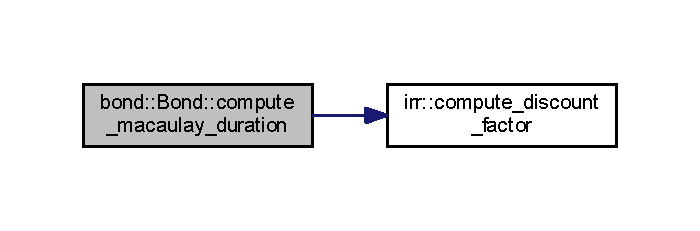
\includegraphics[width=336pt]{classbond_1_1_bond_a57f98f3e281876089945e08457ce6bc6_cgraph}
\end{center}
\end{figure}
\mbox{\Hypertarget{classbond_1_1_bond_ab8a8cfc409d2842e8d9053e53d50468f}\label{classbond_1_1_bond_ab8a8cfc409d2842e8d9053e53d50468f}} 
\index{bond\+::\+Bond@{bond\+::\+Bond}!compute\+\_\+yield@{compute\+\_\+yield}}
\index{compute\+\_\+yield@{compute\+\_\+yield}!bond\+::\+Bond@{bond\+::\+Bond}}
\subsubsection{\texorpdfstring{compute\+\_\+yield()}{compute\_yield()}\hspace{0.1cm}{\footnotesize\ttfamily [1/2]}}
{\footnotesize\ttfamily template$<$typename T $>$ \\
template$<$typename S $>$ \\
T \hyperlink{classbond_1_1_bond}{bond\+::\+Bond}$<$ T $>$\+::compute\+\_\+yield (\begin{DoxyParamCaption}\item[{const T \&}]{i\+\_\+price,  }\item[{const S \&}]{solver,  }\item[{const \hyperlink{namespaceutilities_ad4290e607d0651ce53db6e5c776aca7c}{D\+F\+\_\+type} \&}]{df\+\_\+type }\end{DoxyParamCaption}) const}



Calculates the yield-\/to-\/maturity using the supplied solver. 


\begin{DoxyParams}{Parameters}
{\em i\+\_\+price} & The price of the bond \\
\hline
{\em solver} & The parameter structure of the solver that is going to be used to estimate the yield of maturity \\
\hline
{\em df\+\_\+type} & The type of discount factor method \\
\hline
\end{DoxyParams}
\begin{DoxyReturn}{Returns}
The yield-\/to-\/maturity of the bond 
\end{DoxyReturn}


Definition at line 150 of file bond.\+h.



References irr\+::constraints\+\_\+irr(), irr\+::fitness\+\_\+irr(), and ea\+::solve().


\begin{DoxyCode}
151     \{
152         assert(solver.ndv == 1);
153         \textcolor{keyword}{auto} f = [&,use\_penalty\_method = solver.use\_penalty\_method](\textcolor{keyword}{const} \textcolor{keyword}{auto}& solution) \{ \textcolor{keywordflow}{return} 
      \hyperlink{namespaceirr_aced01c5e5ef9e171a3b892275d442f8d}{fitness\_irr}(solution, i\_price, \hyperlink{classbond_1_1_bond_a7a79ca13c060697765f13140eb471b84}{nominal\_value}, \hyperlink{classbond_1_1_bond_ae98011d18cd97942b45f5868a42bf668}{cash\_flows}, 
      \hyperlink{classbond_1_1_bond_ac3db034ebeff1f6cd2ed7061fda27fad}{time\_periods}, df\_type, use\_penalty\_method); \};
154         \textcolor{keyword}{auto} c = [&,constraints\_type = solver.constraints\_type](\textcolor{keyword}{const} \textcolor{keyword}{auto}& solution) \{ \textcolor{keywordflow}{return} 
      \hyperlink{namespaceirr_a6801aa96a307b3f52817dd1a3bcd065e}{constraints\_irr}(solution, constraints\_type); \};
155         \textcolor{keyword}{auto} res = \hyperlink{namespaceea_a6450b5bf61e9fdca8b6c19267e14c560}{solve}(f, c, solver, \textcolor{stringliteral}{"YTM"});
156         T \hyperlink{classbond_1_1_bond_ac79ec630d68f58775849145ab305d5f8}{yield} = res[0];
157         \textcolor{keywordflow}{return} \hyperlink{classbond_1_1_bond_ac79ec630d68f58775849145ab305d5f8}{yield};
158     \}
\end{DoxyCode}
Here is the call graph for this function\+:
\nopagebreak
\begin{figure}[H]
\begin{center}
\leavevmode
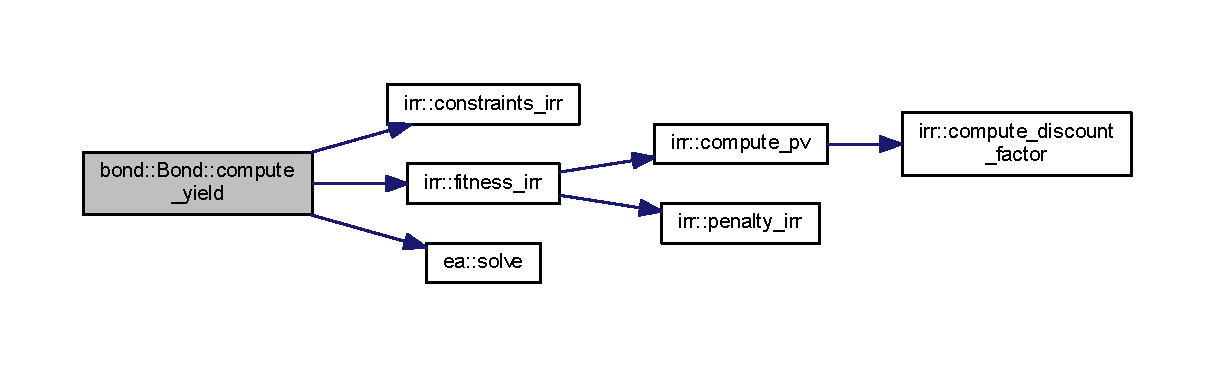
\includegraphics[width=350pt]{classbond_1_1_bond_ab8a8cfc409d2842e8d9053e53d50468f_cgraph}
\end{center}
\end{figure}
\mbox{\Hypertarget{classbond_1_1_bond_ab4dba13e68b2685eef680fe7b8155a7a}\label{classbond_1_1_bond_ab4dba13e68b2685eef680fe7b8155a7a}} 
\index{bond\+::\+Bond@{bond\+::\+Bond}!compute\+\_\+yield@{compute\+\_\+yield}}
\index{compute\+\_\+yield@{compute\+\_\+yield}!bond\+::\+Bond@{bond\+::\+Bond}}
\subsubsection{\texorpdfstring{compute\+\_\+yield()}{compute\_yield()}\hspace{0.1cm}{\footnotesize\ttfamily [2/2]}}
{\footnotesize\ttfamily template$<$typename T $>$ \\
template$<$typename S $>$ \\
T \hyperlink{classbond_1_1_bond}{bond\+::\+Bond}$<$ T $>$\+::compute\+\_\+yield (\begin{DoxyParamCaption}\item[{const T \&}]{i\+\_\+price,  }\item[{const S \&}]{solver,  }\item[{const \hyperlink{namespaceutilities_ad4290e607d0651ce53db6e5c776aca7c}{D\+F\+\_\+type} \&}]{df\+\_\+type,  }\item[{const std\+::string \&}]{bonds\+\_\+identifier }\end{DoxyParamCaption}) const}



Calculates the yield-\/to-\/maturity using the supplied solver and passes the bond identifier to the solver. 


\begin{DoxyParams}{Parameters}
{\em i\+\_\+price} & The price of the bond \\
\hline
{\em solver} & The parameter structure of the solver that is going to be used to estimate the yield of maturity \\
\hline
{\em df\+\_\+type} & The type of discount factor method \\
\hline
{\em bonds\+\_\+identifier} & An identifier for the bond in std\+::string form \\
\hline
\end{DoxyParams}
\begin{DoxyReturn}{Returns}
The yield-\/to-\/maturity of the bond 
\end{DoxyReturn}


Definition at line 162 of file bond.\+h.



References irr\+::constraints\+\_\+irr(), irr\+::fitness\+\_\+irr(), and ea\+::solve().


\begin{DoxyCode}
163     \{
164         assert(solver.ndv == 1);
165         \textcolor{keyword}{auto} f = [&, use\_penalty\_method = solver.use\_penalty\_method](\textcolor{keyword}{const} \textcolor{keyword}{auto}& solution) \{ \textcolor{keywordflow}{return} 
      \hyperlink{namespaceirr_aced01c5e5ef9e171a3b892275d442f8d}{fitness\_irr}(solution, i\_price, \hyperlink{classbond_1_1_bond_a7a79ca13c060697765f13140eb471b84}{nominal\_value}, \hyperlink{classbond_1_1_bond_ae98011d18cd97942b45f5868a42bf668}{cash\_flows}, 
      \hyperlink{classbond_1_1_bond_ac3db034ebeff1f6cd2ed7061fda27fad}{time\_periods}, df\_type, use\_penalty\_method); \};
166         \textcolor{keyword}{auto} c = [&, constraints\_type = solver.constraints\_type](\textcolor{keyword}{const} \textcolor{keyword}{auto}& solution) \{ \textcolor{keywordflow}{return} 
      \hyperlink{namespaceirr_a6801aa96a307b3f52817dd1a3bcd065e}{constraints\_irr}(solution, constraints\_type); \};
167         std::string problem = \textcolor{stringliteral}{"YTM"};
168         \textcolor{keyword}{auto} res = \hyperlink{namespaceea_a6450b5bf61e9fdca8b6c19267e14c560}{solve}(f, c, solver, problem.append(bonds\_identifier));
169         T \hyperlink{classbond_1_1_bond_ac79ec630d68f58775849145ab305d5f8}{yield} = res[0];
170         \textcolor{keywordflow}{return} \hyperlink{classbond_1_1_bond_ac79ec630d68f58775849145ab305d5f8}{yield};
171     \}
\end{DoxyCode}
Here is the call graph for this function\+:
\nopagebreak
\begin{figure}[H]
\begin{center}
\leavevmode
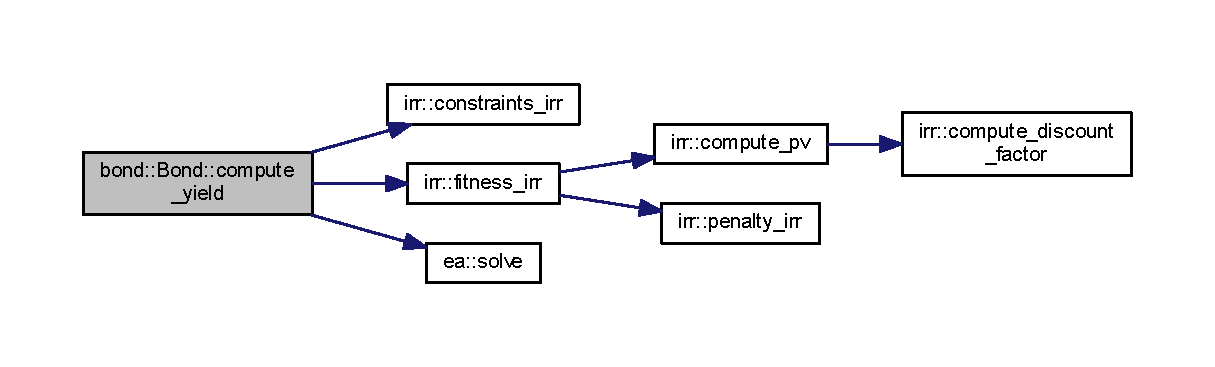
\includegraphics[width=350pt]{classbond_1_1_bond_ab4dba13e68b2685eef680fe7b8155a7a_cgraph}
\end{center}
\end{figure}


\subsection{Friends And Related Function Documentation}
\mbox{\Hypertarget{classbond_1_1_bond_aa0950c8d07f76b3cb69c5655951e1386}\label{classbond_1_1_bond_aa0950c8d07f76b3cb69c5655951e1386}} 
\index{bond\+::\+Bond@{bond\+::\+Bond}!Bond\+Helper$<$ T $>$@{Bond\+Helper$<$ T $>$}}
\index{Bond\+Helper$<$ T $>$@{Bond\+Helper$<$ T $>$}!bond\+::\+Bond@{bond\+::\+Bond}}
\subsubsection{\texorpdfstring{Bond\+Helper$<$ T $>$}{BondHelper< T >}}
{\footnotesize\ttfamily template$<$typename T $>$ \\
friend class \hyperlink{classbond_1_1_bond_helper}{Bond\+Helper}$<$ T $>$\hspace{0.3cm}{\ttfamily [friend]}}



Friend class \hyperlink{classbond_1_1_bond_helper}{Bond\+Helper}. 



Definition at line 35 of file bond.\+h.



\subsection{Member Data Documentation}
\mbox{\Hypertarget{classbond_1_1_bond_ae98011d18cd97942b45f5868a42bf668}\label{classbond_1_1_bond_ae98011d18cd97942b45f5868a42bf668}} 
\index{bond\+::\+Bond@{bond\+::\+Bond}!cash\+\_\+flows@{cash\+\_\+flows}}
\index{cash\+\_\+flows@{cash\+\_\+flows}!bond\+::\+Bond@{bond\+::\+Bond}}
\subsubsection{\texorpdfstring{cash\+\_\+flows}{cash\_flows}}
{\footnotesize\ttfamily template$<$typename T $>$ \\
std\+::vector$<$T$>$ \hyperlink{classbond_1_1_bond}{bond\+::\+Bond}$<$ T $>$\+::cash\+\_\+flows\hspace{0.3cm}{\ttfamily [private]}}



A vector with all the coupon payments corresponding to time periods. 



Definition at line 116 of file bond.\+h.

\mbox{\Hypertarget{classbond_1_1_bond_add6662fd4f8ee756b83a3f818f8c7ada}\label{classbond_1_1_bond_add6662fd4f8ee756b83a3f818f8c7ada}} 
\index{bond\+::\+Bond@{bond\+::\+Bond}!coupon\+\_\+percentage@{coupon\+\_\+percentage}}
\index{coupon\+\_\+percentage@{coupon\+\_\+percentage}!bond\+::\+Bond@{bond\+::\+Bond}}
\subsubsection{\texorpdfstring{coupon\+\_\+percentage}{coupon\_percentage}}
{\footnotesize\ttfamily template$<$typename T $>$ \\
const T \hyperlink{classbond_1_1_bond}{bond\+::\+Bond}$<$ T $>$\+::coupon\+\_\+percentage\hspace{0.3cm}{\ttfamily [private]}}



\hyperlink{classbond_1_1_bond}{Bond}\textquotesingle{}s annual coupon rate. 



Definition at line 104 of file bond.\+h.

\mbox{\Hypertarget{classbond_1_1_bond_aae68bdfac23a0530b3723cca3100e92e}\label{classbond_1_1_bond_aae68bdfac23a0530b3723cca3100e92e}} 
\index{bond\+::\+Bond@{bond\+::\+Bond}!coupon\+\_\+value@{coupon\+\_\+value}}
\index{coupon\+\_\+value@{coupon\+\_\+value}!bond\+::\+Bond@{bond\+::\+Bond}}
\subsubsection{\texorpdfstring{coupon\+\_\+value}{coupon\_value}}
{\footnotesize\ttfamily template$<$typename T $>$ \\
const T \hyperlink{classbond_1_1_bond}{bond\+::\+Bond}$<$ T $>$\+::coupon\+\_\+value\hspace{0.3cm}{\ttfamily [private]}}



This is the annual coupon divided by the frequency. 



Definition at line 112 of file bond.\+h.

\mbox{\Hypertarget{classbond_1_1_bond_a76d054bdd6dcdefa0147495f8ecdc852}\label{classbond_1_1_bond_a76d054bdd6dcdefa0147495f8ecdc852}} 
\index{bond\+::\+Bond@{bond\+::\+Bond}!duration@{duration}}
\index{duration@{duration}!bond\+::\+Bond@{bond\+::\+Bond}}
\subsubsection{\texorpdfstring{duration}{duration}}
{\footnotesize\ttfamily template$<$typename T $>$ \\
T \hyperlink{classbond_1_1_bond}{bond\+::\+Bond}$<$ T $>$\+::duration\hspace{0.3cm}{\ttfamily [private]}}



Macaulay duration of the bond. 



Definition at line 124 of file bond.\+h.

\mbox{\Hypertarget{classbond_1_1_bond_ad1871f40122a63fb0b2ebbdcdd12c1cd}\label{classbond_1_1_bond_ad1871f40122a63fb0b2ebbdcdd12c1cd}} 
\index{bond\+::\+Bond@{bond\+::\+Bond}!frequency@{frequency}}
\index{frequency@{frequency}!bond\+::\+Bond@{bond\+::\+Bond}}
\subsubsection{\texorpdfstring{frequency}{frequency}}
{\footnotesize\ttfamily template$<$typename T $>$ \\
const T \hyperlink{classbond_1_1_bond}{bond\+::\+Bond}$<$ T $>$\+::frequency\hspace{0.3cm}{\ttfamily [private]}}



\hyperlink{classbond_1_1_bond}{Bond}\textquotesingle{}s coupon payment frequency. 



Definition at line 110 of file bond.\+h.

\mbox{\Hypertarget{classbond_1_1_bond_aba0bd9e2e1de7b9f05bb9c61b1fb9f1e}\label{classbond_1_1_bond_aba0bd9e2e1de7b9f05bb9c61b1fb9f1e}} 
\index{bond\+::\+Bond@{bond\+::\+Bond}!maturity\+\_\+date@{maturity\+\_\+date}}
\index{maturity\+\_\+date@{maturity\+\_\+date}!bond\+::\+Bond@{bond\+::\+Bond}}
\subsubsection{\texorpdfstring{maturity\+\_\+date}{maturity\_date}}
{\footnotesize\ttfamily template$<$typename T $>$ \\
date\+::sys\+\_\+days \hyperlink{classbond_1_1_bond}{bond\+::\+Bond}$<$ T $>$\+::maturity\+\_\+date\hspace{0.3cm}{\ttfamily [private]}}



Maturity date of the bond. 



Definition at line 120 of file bond.\+h.

\mbox{\Hypertarget{classbond_1_1_bond_a7a79ca13c060697765f13140eb471b84}\label{classbond_1_1_bond_a7a79ca13c060697765f13140eb471b84}} 
\index{bond\+::\+Bond@{bond\+::\+Bond}!nominal\+\_\+value@{nominal\+\_\+value}}
\index{nominal\+\_\+value@{nominal\+\_\+value}!bond\+::\+Bond@{bond\+::\+Bond}}
\subsubsection{\texorpdfstring{nominal\+\_\+value}{nominal\_value}}
{\footnotesize\ttfamily template$<$typename T $>$ \\
const T \hyperlink{classbond_1_1_bond}{bond\+::\+Bond}$<$ T $>$\+::nominal\+\_\+value\hspace{0.3cm}{\ttfamily [private]}}



\hyperlink{classbond_1_1_bond}{Bond}\textquotesingle{}s face value. 



Definition at line 108 of file bond.\+h.

\mbox{\Hypertarget{classbond_1_1_bond_afcabe8593aba44ca9740d14f85a39f2a}\label{classbond_1_1_bond_afcabe8593aba44ca9740d14f85a39f2a}} 
\index{bond\+::\+Bond@{bond\+::\+Bond}!price@{price}}
\index{price@{price}!bond\+::\+Bond@{bond\+::\+Bond}}
\subsubsection{\texorpdfstring{price}{price}}
{\footnotesize\ttfamily template$<$typename T $>$ \\
const T \hyperlink{classbond_1_1_bond}{bond\+::\+Bond}$<$ T $>$\+::price\hspace{0.3cm}{\ttfamily [private]}}



\hyperlink{classbond_1_1_bond}{Bond}\textquotesingle{}s price. 



Definition at line 106 of file bond.\+h.

\mbox{\Hypertarget{classbond_1_1_bond_a2ead15c4c0cbda2cdecf6500b02442e7}\label{classbond_1_1_bond_a2ead15c4c0cbda2cdecf6500b02442e7}} 
\index{bond\+::\+Bond@{bond\+::\+Bond}!settlement\+\_\+date@{settlement\+\_\+date}}
\index{settlement\+\_\+date@{settlement\+\_\+date}!bond\+::\+Bond@{bond\+::\+Bond}}
\subsubsection{\texorpdfstring{settlement\+\_\+date}{settlement\_date}}
{\footnotesize\ttfamily template$<$typename T $>$ \\
date\+::sys\+\_\+days \hyperlink{classbond_1_1_bond}{bond\+::\+Bond}$<$ T $>$\+::settlement\+\_\+date\hspace{0.3cm}{\ttfamily [private]}}



Settlement date of the bond. 



Definition at line 118 of file bond.\+h.

\mbox{\Hypertarget{classbond_1_1_bond_ac3db034ebeff1f6cd2ed7061fda27fad}\label{classbond_1_1_bond_ac3db034ebeff1f6cd2ed7061fda27fad}} 
\index{bond\+::\+Bond@{bond\+::\+Bond}!time\+\_\+periods@{time\+\_\+periods}}
\index{time\+\_\+periods@{time\+\_\+periods}!bond\+::\+Bond@{bond\+::\+Bond}}
\subsubsection{\texorpdfstring{time\+\_\+periods}{time\_periods}}
{\footnotesize\ttfamily template$<$typename T $>$ \\
std\+::vector$<$T$>$ \hyperlink{classbond_1_1_bond}{bond\+::\+Bond}$<$ T $>$\+::time\+\_\+periods\hspace{0.3cm}{\ttfamily [private]}}



Coupon payment periods. 



Definition at line 114 of file bond.\+h.

\mbox{\Hypertarget{classbond_1_1_bond_ac79ec630d68f58775849145ab305d5f8}\label{classbond_1_1_bond_ac79ec630d68f58775849145ab305d5f8}} 
\index{bond\+::\+Bond@{bond\+::\+Bond}!yield@{yield}}
\index{yield@{yield}!bond\+::\+Bond@{bond\+::\+Bond}}
\subsubsection{\texorpdfstring{yield}{yield}}
{\footnotesize\ttfamily template$<$typename T $>$ \\
T \hyperlink{classbond_1_1_bond}{bond\+::\+Bond}$<$ T $>$\+::yield\hspace{0.3cm}{\ttfamily [private]}}



Yield-\/to-\/maturity of the bond. 



Definition at line 122 of file bond.\+h.



The documentation for this class was generated from the following file\+:\begin{DoxyCompactItemize}
\item 
\hyperlink{bond_8h}{bond.\+h}\end{DoxyCompactItemize}

\hypertarget{classbond_1_1_bond_helper}{}\section{bond\+:\+:Bond\+Helper$<$ T $>$ Class Template Reference}
\label{classbond_1_1_bond_helper}\index{bond\+::\+Bond\+Helper$<$ T $>$@{bond\+::\+Bond\+Helper$<$ T $>$}}


A class for the bond pricing problem as well as finding the yield-\/to-\/maturities of bonds.  




{\ttfamily \#include $<$bond.\+h$>$}

\subsection*{Public Member Functions}
\begin{DoxyCompactItemize}
\item 
\hyperlink{classbond_1_1_bond_helper_aa86a95eaffb5a36c0ec52376b28d5d96}{Bond\+Helper} (const std\+::vector$<$ \hyperlink{classbond_1_1_bond}{Bond}$<$ T $>$$>$ \&i\+\_\+bonds, const \hyperlink{namespaceutilities_ad4290e607d0651ce53db6e5c776aca7c}{D\+F\+\_\+type} \&i\+\_\+df\+\_\+type)
\begin{DoxyCompactList}\small\item\em Constructor. \end{DoxyCompactList}\item 
{\footnotesize template$<$typename S $>$ }\\std\+::vector$<$ T $>$ \hyperlink{classbond_1_1_bond_helper_aaf31152498dbbf3704839a0c57e4555c}{set\+\_\+init\+\_\+nss\+\_\+params} (const S \&solver)
\begin{DoxyCompactList}\small\item\em This method sets the nss initial svensson parameters by computing the bond yields-\/to-\/maturity and Macaulay durations. \end{DoxyCompactList}\item 
{\footnotesize template$<$typename S1 , typename S2 $>$ }\\void \hyperlink{classbond_1_1_bond_helper_a160a6bba890e45968d11d887ff34e294}{bond\+\_\+pricing} (const S1 \&solver, const S2 \&solver\+\_\+irr, const \hyperlink{namespacebond_a7ff8132c72465682a65a634ca0958df9}{Bond\+\_\+pricing\+\_\+type} \&bond\+\_\+pricing\+\_\+type)
\begin{DoxyCompactList}\small\item\em This methods solves the bond pricing problem using prices or yields and the supplied solver. \end{DoxyCompactList}\item 
{\footnotesize template$<$typename S $>$ }\\void \hyperlink{classbond_1_1_bond_helper_a28159ce3ba6b11611d6368fd5a601f45}{print\+\_\+bond\+\_\+pricing\+\_\+results} (const std\+::vector$<$ T $>$ \&res, const S \&solver\+\_\+irr)
\begin{DoxyCompactList}\small\item\em This method prints to screen the bond pricing results. \end{DoxyCompactList}\end{DoxyCompactItemize}
\subsection*{Private Member Functions}
\begin{DoxyCompactItemize}
\item 
T \hyperlink{classbond_1_1_bond_helper_a1288528021e7c60e3a1435d39ad8611d}{estimate\+\_\+bond\+\_\+pricing} (const std\+::vector$<$ T $>$ \&solution, const T \&coupon\+\_\+value, const T \&nominal\+\_\+value, const std\+::vector$<$ T $>$ \&time\+\_\+periods)
\begin{DoxyCompactList}\small\item\em Returns the bond prices using the estimated spot interest rates computed with svensson. \end{DoxyCompactList}\item 
{\footnotesize template$<$typename S $>$ }\\T \hyperlink{classbond_1_1_bond_helper_aa1a47c41374aee7914e9c0ac374b39e4}{fitness\+\_\+bond\+\_\+pricing\+\_\+yields} (const std\+::vector$<$ T $>$ \&solution, const S \&solver\+\_\+irr, const bool \&use\+\_\+penalty\+\_\+method)
\begin{DoxyCompactList}\small\item\em This is the fitness function for bond pricing using the bonds\textquotesingle{} yields-\/to-\/maturity. \end{DoxyCompactList}\item 
T \hyperlink{classbond_1_1_bond_helper_a507eddab3d55ad3e640dfa930dcf43d0}{fitness\+\_\+bond\+\_\+pricing\+\_\+prices} (const std\+::vector$<$ T $>$ \&solution, const bool \&use\+\_\+penalty\+\_\+method)
\begin{DoxyCompactList}\small\item\em This is the fitness function for bond pricing using the bonds\textquotesingle{} prices. \end{DoxyCompactList}\end{DoxyCompactItemize}
\subsection*{Private Attributes}
\begin{DoxyCompactItemize}
\item 
std\+::vector$<$ \hyperlink{classbond_1_1_bond}{Bond}$<$ T $>$ $>$ \hyperlink{classbond_1_1_bond_helper_a61db751f82d46ce2f7f5032ff2a3b03e}{bonds}
\begin{DoxyCompactList}\small\item\em Vector of bonds. \end{DoxyCompactList}\item 
const \hyperlink{namespaceutilities_ad4290e607d0651ce53db6e5c776aca7c}{D\+F\+\_\+type} \hyperlink{classbond_1_1_bond_helper_a843e3c12a561aaac047ba70310375a2f}{df\+\_\+type}
\begin{DoxyCompactList}\small\item\em Discount Factor type. \end{DoxyCompactList}\end{DoxyCompactItemize}


\subsection{Detailed Description}
\subsubsection*{template$<$typename T$>$\newline
class bond\+::\+Bond\+Helper$<$ T $>$}

A class for the bond pricing problem as well as finding the yield-\/to-\/maturities of bonds. 

Definition at line 26 of file bond.\+h.



\subsection{Constructor \& Destructor Documentation}
\mbox{\Hypertarget{classbond_1_1_bond_helper_aa86a95eaffb5a36c0ec52376b28d5d96}\label{classbond_1_1_bond_helper_aa86a95eaffb5a36c0ec52376b28d5d96}} 
\index{bond\+::\+Bond\+Helper@{bond\+::\+Bond\+Helper}!Bond\+Helper@{Bond\+Helper}}
\index{Bond\+Helper@{Bond\+Helper}!bond\+::\+Bond\+Helper@{bond\+::\+Bond\+Helper}}
\subsubsection{\texorpdfstring{Bond\+Helper()}{BondHelper()}}
{\footnotesize\ttfamily template$<$typename T $>$ \\
\hyperlink{classbond_1_1_bond_helper}{bond\+::\+Bond\+Helper}$<$ T $>$\+::\hyperlink{classbond_1_1_bond_helper}{Bond\+Helper} (\begin{DoxyParamCaption}\item[{const std\+::vector$<$ \hyperlink{classbond_1_1_bond}{Bond}$<$ T $>$$>$ \&}]{i\+\_\+bonds,  }\item[{const \hyperlink{namespaceutilities_ad4290e607d0651ce53db6e5c776aca7c}{D\+F\+\_\+type} \&}]{i\+\_\+df\+\_\+type = {\ttfamily DF\+\_\+type\+:\+:exp} }\end{DoxyParamCaption})\hspace{0.3cm}{\ttfamily [inline]}}



Constructor. 


\begin{DoxyParams}{Parameters}
{\em i\+\_\+bonds} & A vector of Bond$<$\+T$>$ objects \\
\hline
{\em i\+\_\+df\+\_\+type} & The type of discount factor method \\
\hline
\end{DoxyParams}
\begin{DoxyReturn}{Returns}
A Bond\+Helper$<$\+T$>$ object 
\end{DoxyReturn}


Definition at line 66 of file bondhelper.\+h.


\begin{DoxyCode}
66                                                                                 : 
67             \hyperlink{classbond_1_1_bond_helper_a61db751f82d46ce2f7f5032ff2a3b03e}{bonds}( i\_bonds ), 
68             \hyperlink{classbond_1_1_bond_helper_a843e3c12a561aaac047ba70310375a2f}{df\_type}( i\_df\_type )
69         \{\};
\end{DoxyCode}


\subsection{Member Function Documentation}
\mbox{\Hypertarget{classbond_1_1_bond_helper_a160a6bba890e45968d11d887ff34e294}\label{classbond_1_1_bond_helper_a160a6bba890e45968d11d887ff34e294}} 
\index{bond\+::\+Bond\+Helper@{bond\+::\+Bond\+Helper}!bond\+\_\+pricing@{bond\+\_\+pricing}}
\index{bond\+\_\+pricing@{bond\+\_\+pricing}!bond\+::\+Bond\+Helper@{bond\+::\+Bond\+Helper}}
\subsubsection{\texorpdfstring{bond\+\_\+pricing()}{bond\_pricing()}}
{\footnotesize\ttfamily template$<$typename T $>$ \\
template$<$typename S1 , typename S2 $>$ \\
void \hyperlink{classbond_1_1_bond_helper}{bond\+::\+Bond\+Helper}$<$ T $>$\+::bond\+\_\+pricing (\begin{DoxyParamCaption}\item[{const S1 \&}]{solver,  }\item[{const S2 \&}]{solver\+\_\+irr,  }\item[{const \hyperlink{namespacebond_a7ff8132c72465682a65a634ca0958df9}{Bond\+\_\+pricing\+\_\+type} \&}]{bond\+\_\+pricing\+\_\+type }\end{DoxyParamCaption})}



This methods solves the bond pricing problem using prices or yields and the supplied solver. 


\begin{DoxyParams}{Parameters}
{\em solver} & The parameter structure of the solver that is going to be used for bond pricing \\
\hline
{\em solver\+\_\+irr} & The parameter structure of the solver that is going to be used to estimate the yield of maturity \\
\hline
{\em bond\+\_\+pricing\+\_\+type} & Whether to use bond yields-\/to-\/maturities or bond prices to find the N\+SS parameters \\
\hline
\end{DoxyParams}
\begin{DoxyReturn}{Returns}
void 
\end{DoxyReturn}


Definition at line 235 of file bondhelper.\+h.



References bond\+::bpp, bond\+::bpy, nss\+::constraints\+\_\+svensson(), and ea\+::solve().


\begin{DoxyCode}
236     \{
237         assert(solver.ndv == 6);
238         \textcolor{keywordflow}{for} (\textcolor{keyword}{const} \textcolor{keyword}{auto}& p : \hyperlink{classbond_1_1_bond_helper_a61db751f82d46ce2f7f5032ff2a3b03e}{bonds})
239         \{
240             assert(p.yield > 0 && p.yield < 1);
241             assert(p.duration > 0);
242         \}
243         \textcolor{keywordflow}{switch} (bond\_pricing\_type)
244         \{
245         \textcolor{keywordflow}{case}(\hyperlink{namespacebond_a7ff8132c72465682a65a634ca0958df9a0c68c2daa0334704116676287d54c2ae}{Bond\_pricing\_type::bpp}):
246         \{
247             \textcolor{keyword}{auto} f = [&, use\_penalty\_method = solver.use\_penalty\_method](\textcolor{keyword}{const} \textcolor{keyword}{auto}& solution) \{ \textcolor{keywordflow}{return} 
      \hyperlink{classbond_1_1_bond_helper_a507eddab3d55ad3e640dfa930dcf43d0}{fitness\_bond\_pricing\_prices}(solution, use\_penalty\_method); \};
248             \textcolor{keyword}{auto} c = [&, constraints\_type = solver.constraints\_type](\textcolor{keyword}{const} \textcolor{keyword}{auto}& solution) \{ \textcolor{keywordflow}{return} 
      \hyperlink{namespacenss_a39de3569a71e773f9da82c713eb7e6eb}{constraints\_svensson}(solution, constraints\_type); \};
249             std::cout << \textcolor{stringliteral}{"Solving bond pricing using bond prices..."} << \textcolor{stringliteral}{"\(\backslash\)n"};
250             \textcolor{keyword}{auto} res = \hyperlink{namespaceea_a6450b5bf61e9fdca8b6c19267e14c560}{solve}(f, c, solver, \textcolor{stringliteral}{"BPP"});
251             \hyperlink{classbond_1_1_bond_helper_a28159ce3ba6b11611d6368fd5a601f45}{print\_bond\_pricing\_results}(res, solver\_irr);
252             \textcolor{keywordflow}{break};
253         \}
254         \textcolor{keywordflow}{case}(\hyperlink{namespacebond_a7ff8132c72465682a65a634ca0958df9afebbcc7d14e1ada7b0eee6411e82665b}{Bond\_pricing\_type::bpy}):
255         \{
256             \textcolor{keyword}{auto} f = [&, use\_penalty\_method = solver.use\_penalty\_method](\textcolor{keyword}{const} \textcolor{keyword}{auto}& solution) \{ \textcolor{keywordflow}{return} 
      \hyperlink{classbond_1_1_bond_helper_aa1a47c41374aee7914e9c0ac374b39e4}{fitness\_bond\_pricing\_yields}(solution, solver\_irr, use\_penalty\_method); \};
257             \textcolor{keyword}{auto} c = [&, constraints\_type = solver.constraints\_type](\textcolor{keyword}{const} \textcolor{keyword}{auto}& solution) \{ \textcolor{keywordflow}{return} 
      \hyperlink{namespacenss_a39de3569a71e773f9da82c713eb7e6eb}{constraints\_svensson}(solution, constraints\_type); \};
258             std::cout << \textcolor{stringliteral}{"Solving bond pricing using bond yields..."} << \textcolor{stringliteral}{"\(\backslash\)n"};
259             \textcolor{keyword}{auto} res = \hyperlink{namespaceea_a6450b5bf61e9fdca8b6c19267e14c560}{solve}(f, c, solver, \textcolor{stringliteral}{"BPY"});
260             \hyperlink{classbond_1_1_bond_helper_a28159ce3ba6b11611d6368fd5a601f45}{print\_bond\_pricing\_results}(res, solver\_irr);
261         \}
262         \}
263     \}
\end{DoxyCode}
Here is the call graph for this function\+:
\nopagebreak
\begin{figure}[H]
\begin{center}
\leavevmode
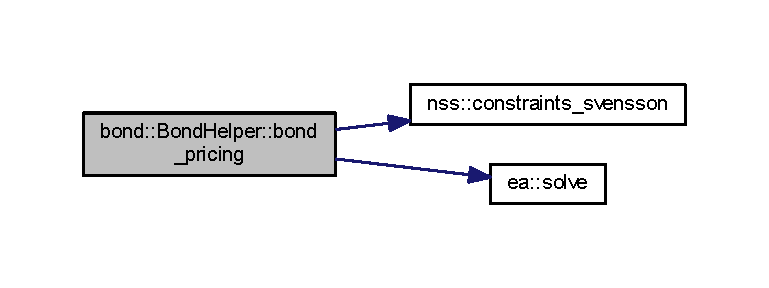
\includegraphics[width=350pt]{classbond_1_1_bond_helper_a160a6bba890e45968d11d887ff34e294_cgraph}
\end{center}
\end{figure}
\mbox{\Hypertarget{classbond_1_1_bond_helper_a1288528021e7c60e3a1435d39ad8611d}\label{classbond_1_1_bond_helper_a1288528021e7c60e3a1435d39ad8611d}} 
\index{bond\+::\+Bond\+Helper@{bond\+::\+Bond\+Helper}!estimate\+\_\+bond\+\_\+pricing@{estimate\+\_\+bond\+\_\+pricing}}
\index{estimate\+\_\+bond\+\_\+pricing@{estimate\+\_\+bond\+\_\+pricing}!bond\+::\+Bond\+Helper@{bond\+::\+Bond\+Helper}}
\subsubsection{\texorpdfstring{estimate\+\_\+bond\+\_\+pricing()}{estimate\_bond\_pricing()}}
{\footnotesize\ttfamily template$<$typename T $>$ \\
T \hyperlink{classbond_1_1_bond_helper}{bond\+::\+Bond\+Helper}$<$ T $>$\+::estimate\+\_\+bond\+\_\+pricing (\begin{DoxyParamCaption}\item[{const std\+::vector$<$ T $>$ \&}]{solution,  }\item[{const T \&}]{coupon\+\_\+value,  }\item[{const T \&}]{nominal\+\_\+value,  }\item[{const std\+::vector$<$ T $>$ \&}]{time\+\_\+periods }\end{DoxyParamCaption})\hspace{0.3cm}{\ttfamily [private]}}



Returns the bond prices using the estimated spot interest rates computed with svensson. 


\begin{DoxyParams}{Parameters}
{\em solution} & N\+SS parameters candindate solution \\
\hline
{\em coupon\+\_\+value} & The value of the coupon payment \\
\hline
{\em nominal\+\_\+value} & The nominal value of the investment \\
\hline
{\em time\+\_\+periods} & The time periods that correspond to the coupon payments \\
\hline
\end{DoxyParams}
\begin{DoxyReturn}{Returns}
The price of the bond 
\end{DoxyReturn}
Call svensson for period 

Definition at line 178 of file bondhelper.\+h.



References irr\+::compute\+\_\+discount\+\_\+factor(), and nss\+::svensson().


\begin{DoxyCode}
179     \{
180         T sum = 0.0;
182         \textcolor{keywordflow}{for} (\textcolor{keyword}{const} \textcolor{keyword}{auto}& t : time\_periods)
183         \{
184             sum = sum + coupon\_value * \hyperlink{namespaceirr_ae00c3409ca39fa2dc47ce61da4169a66}{compute\_discount\_factor}(
      \hyperlink{namespacenss_a71aad246261afa16f8bb1a4057570d4b}{svensson}(solution, t), t, \hyperlink{classbond_1_1_bond_helper_a843e3c12a561aaac047ba70310375a2f}{df\_type});
185         \}       
186         T m = time\_periods.back();
187         sum = sum + nominal\_value * \hyperlink{namespaceirr_ae00c3409ca39fa2dc47ce61da4169a66}{compute\_discount\_factor}(
      \hyperlink{namespacenss_a71aad246261afa16f8bb1a4057570d4b}{svensson}(solution, m), m, \hyperlink{classbond_1_1_bond_helper_a843e3c12a561aaac047ba70310375a2f}{df\_type});
188         \textcolor{keywordflow}{return} sum;
189     \}
\end{DoxyCode}
Here is the call graph for this function\+:
\nopagebreak
\begin{figure}[H]
\begin{center}
\leavevmode
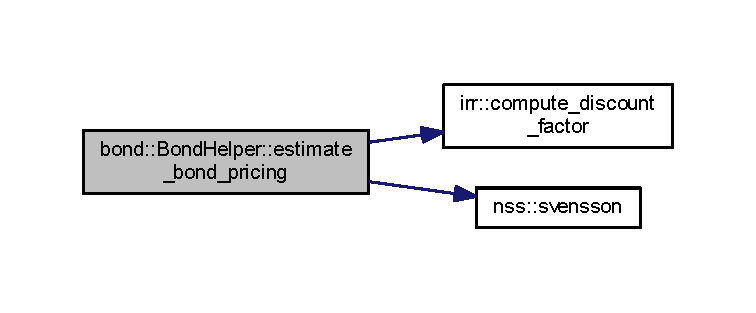
\includegraphics[width=350pt]{classbond_1_1_bond_helper_a1288528021e7c60e3a1435d39ad8611d_cgraph}
\end{center}
\end{figure}
\mbox{\Hypertarget{classbond_1_1_bond_helper_a507eddab3d55ad3e640dfa930dcf43d0}\label{classbond_1_1_bond_helper_a507eddab3d55ad3e640dfa930dcf43d0}} 
\index{bond\+::\+Bond\+Helper@{bond\+::\+Bond\+Helper}!fitness\+\_\+bond\+\_\+pricing\+\_\+prices@{fitness\+\_\+bond\+\_\+pricing\+\_\+prices}}
\index{fitness\+\_\+bond\+\_\+pricing\+\_\+prices@{fitness\+\_\+bond\+\_\+pricing\+\_\+prices}!bond\+::\+Bond\+Helper@{bond\+::\+Bond\+Helper}}
\subsubsection{\texorpdfstring{fitness\+\_\+bond\+\_\+pricing\+\_\+prices()}{fitness\_bond\_pricing\_prices()}}
{\footnotesize\ttfamily template$<$typename T $>$ \\
T \hyperlink{classbond_1_1_bond_helper}{bond\+::\+Bond\+Helper}$<$ T $>$\+::fitness\+\_\+bond\+\_\+pricing\+\_\+prices (\begin{DoxyParamCaption}\item[{const std\+::vector$<$ T $>$ \&}]{solution,  }\item[{const bool \&}]{use\+\_\+penalty\+\_\+method }\end{DoxyParamCaption})\hspace{0.3cm}{\ttfamily [private]}}



This is the fitness function for bond pricing using the bonds\textquotesingle{} prices. 


\begin{DoxyParams}{Parameters}
{\em solution} & N\+SS parameters candindate solution \\
\hline
{\em use\+\_\+penalty\+\_\+method} & Whether to use the penalty method defined for N\+SS or not \\
\hline
\end{DoxyParams}
\begin{DoxyReturn}{Returns}
The fitness cost of N\+SS for bond pricing 
\end{DoxyReturn}
The sum of squares of errors between the actual bond price and the estimated price from estimate\+\_\+bond\+\_\+pricing 

Definition at line 192 of file bondhelper.\+h.



References nss\+::penalty\+\_\+svensson().


\begin{DoxyCode}
193     \{
195         T sum\_of\_squares = 0.0;
196         \textcolor{keywordflow}{for} (\textcolor{keyword}{const} \textcolor{keyword}{auto}& k : \hyperlink{classbond_1_1_bond_helper_a61db751f82d46ce2f7f5032ff2a3b03e}{bonds})
197         \{
198             T estimate = \hyperlink{classbond_1_1_bond_helper_a1288528021e7c60e3a1435d39ad8611d}{estimate\_bond\_pricing}(solution, k.coupon\_value, k.
      nominal\_value, k.time\_periods);
199             sum\_of\_squares = sum\_of\_squares + std::pow((k.price/100 - estimate/100), 2) / std::sqrt(k.
      duration);
200         \}
201         \textcolor{keywordflow}{if} (use\_penalty\_method)
202         \{
203             \textcolor{keywordflow}{return} sum\_of\_squares + \hyperlink{namespacenss_a009a0ebbca20f7969d0c2ed5a241aa82}{penalty\_svensson}(solution);
204         \}
205         \textcolor{keywordflow}{else}
206         \{
207             \textcolor{keywordflow}{return} sum\_of\_squares;
208         \}
209     \}
\end{DoxyCode}
Here is the call graph for this function\+:
\nopagebreak
\begin{figure}[H]
\begin{center}
\leavevmode
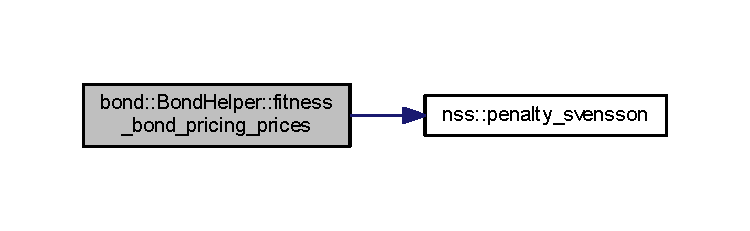
\includegraphics[width=350pt]{classbond_1_1_bond_helper_a507eddab3d55ad3e640dfa930dcf43d0_cgraph}
\end{center}
\end{figure}
\mbox{\Hypertarget{classbond_1_1_bond_helper_aa1a47c41374aee7914e9c0ac374b39e4}\label{classbond_1_1_bond_helper_aa1a47c41374aee7914e9c0ac374b39e4}} 
\index{bond\+::\+Bond\+Helper@{bond\+::\+Bond\+Helper}!fitness\+\_\+bond\+\_\+pricing\+\_\+yields@{fitness\+\_\+bond\+\_\+pricing\+\_\+yields}}
\index{fitness\+\_\+bond\+\_\+pricing\+\_\+yields@{fitness\+\_\+bond\+\_\+pricing\+\_\+yields}!bond\+::\+Bond\+Helper@{bond\+::\+Bond\+Helper}}
\subsubsection{\texorpdfstring{fitness\+\_\+bond\+\_\+pricing\+\_\+yields()}{fitness\_bond\_pricing\_yields()}}
{\footnotesize\ttfamily template$<$typename T $>$ \\
template$<$typename S $>$ \\
T \hyperlink{classbond_1_1_bond_helper}{bond\+::\+Bond\+Helper}$<$ T $>$\+::fitness\+\_\+bond\+\_\+pricing\+\_\+yields (\begin{DoxyParamCaption}\item[{const std\+::vector$<$ T $>$ \&}]{solution,  }\item[{const S \&}]{solver\+\_\+irr,  }\item[{const bool \&}]{use\+\_\+penalty\+\_\+method }\end{DoxyParamCaption})\hspace{0.3cm}{\ttfamily [private]}}



This is the fitness function for bond pricing using the bonds\textquotesingle{} yields-\/to-\/maturity. 


\begin{DoxyParams}{Parameters}
{\em solution} & N\+SS parameters candindate solution \\
\hline
{\em solver\+\_\+irr} & The parameter structure of the solver that is going to be used to estimate the yield of maturity \\
\hline
{\em use\+\_\+penalty\+\_\+method} & Whether to use the penalty method defined for N\+SS or not \\
\hline
\end{DoxyParams}
\begin{DoxyReturn}{Returns}
The fitness cost of N\+SS for bond pricing 
\end{DoxyReturn}
The sum of squares of errors between the actual bond yield to maturity and the estimated yield to maturity by svensson is used 

Definition at line 213 of file bondhelper.\+h.



References nss\+::penalty\+\_\+svensson().


\begin{DoxyCode}
214     \{
216         T sum\_of\_squares = 0;
217         \textcolor{keywordflow}{for} (\textcolor{keyword}{const} \textcolor{keyword}{auto}& k : \hyperlink{classbond_1_1_bond_helper_a61db751f82d46ce2f7f5032ff2a3b03e}{bonds})
218         \{
219             T estimate\_price = \hyperlink{classbond_1_1_bond_helper_a1288528021e7c60e3a1435d39ad8611d}{estimate\_bond\_pricing}(solution, k.coupon\_value, k.
      nominal\_value, k.time\_periods);
220             T estimate = k.compute\_yield(estimate\_price, solver\_irr, \hyperlink{classbond_1_1_bond_helper_a843e3c12a561aaac047ba70310375a2f}{df\_type});
221             sum\_of\_squares = sum\_of\_squares + std::pow(k.yield - estimate, 2);
222         \}
223         \textcolor{keywordflow}{if} (use\_penalty\_method)
224         \{
225             \textcolor{keywordflow}{return} sum\_of\_squares + \hyperlink{namespacenss_a009a0ebbca20f7969d0c2ed5a241aa82}{penalty\_svensson}(solution);
226         \}
227         \textcolor{keywordflow}{else}
228         \{
229             \textcolor{keywordflow}{return} sum\_of\_squares;
230         \}
231     \}
\end{DoxyCode}
Here is the call graph for this function\+:
\nopagebreak
\begin{figure}[H]
\begin{center}
\leavevmode
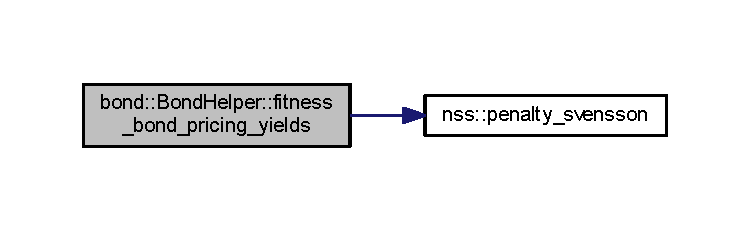
\includegraphics[width=350pt]{classbond_1_1_bond_helper_aa1a47c41374aee7914e9c0ac374b39e4_cgraph}
\end{center}
\end{figure}
\mbox{\Hypertarget{classbond_1_1_bond_helper_a28159ce3ba6b11611d6368fd5a601f45}\label{classbond_1_1_bond_helper_a28159ce3ba6b11611d6368fd5a601f45}} 
\index{bond\+::\+Bond\+Helper@{bond\+::\+Bond\+Helper}!print\+\_\+bond\+\_\+pricing\+\_\+results@{print\+\_\+bond\+\_\+pricing\+\_\+results}}
\index{print\+\_\+bond\+\_\+pricing\+\_\+results@{print\+\_\+bond\+\_\+pricing\+\_\+results}!bond\+::\+Bond\+Helper@{bond\+::\+Bond\+Helper}}
\subsubsection{\texorpdfstring{print\+\_\+bond\+\_\+pricing\+\_\+results()}{print\_bond\_pricing\_results()}}
{\footnotesize\ttfamily template$<$typename T $>$ \\
template$<$typename S $>$ \\
void \hyperlink{classbond_1_1_bond_helper}{bond\+::\+Bond\+Helper}$<$ T $>$\+::print\+\_\+bond\+\_\+pricing\+\_\+results (\begin{DoxyParamCaption}\item[{const std\+::vector$<$ T $>$ \&}]{res,  }\item[{const S \&}]{solver\+\_\+irr }\end{DoxyParamCaption})}



This method prints to screen the bond pricing results. 


\begin{DoxyParams}{Parameters}
{\em res} & The solution vector of N\+SS parameters \\
\hline
{\em solver\+\_\+irr} & The parameter structure of the solver that is going to be used to estimate the yield of maturity \\
\hline
\end{DoxyParams}
\begin{DoxyReturn}{Returns}
void 
\end{DoxyReturn}


Definition at line 267 of file bondhelper.\+h.


\begin{DoxyCode}
268     \{
269         T error = 0;
270         \textcolor{comment}{//for (const auto& p : bonds)}
271         \textcolor{comment}{//\{}
272             \textcolor{comment}{//T estimate\_price = estimate\_bond\_pricing(res, p.coupon\_value, p.nominal\_value,
       p.time\_periods);}
273             \textcolor{comment}{//T estimate = p.compute\_yield(estimate\_price, solver\_irr, df\_type);}
274             \textcolor{comment}{//error = error + std::pow(estimate - p.yield, 2);}
275             \textcolor{comment}{//std::cout << "Estimated yield: " << estimate << " Actual Yield: " << p.yield << "\(\backslash\)n";}
276         \textcolor{comment}{//\}}
277         \textcolor{comment}{//std::cout << "Yield Mean Squared Error: " << error << "\(\backslash\)n";}
278         error = 0;
279         \textcolor{keywordflow}{for} (\textcolor{keyword}{const} \textcolor{keyword}{auto}& p : \hyperlink{classbond_1_1_bond_helper_a61db751f82d46ce2f7f5032ff2a3b03e}{bonds})
280         \{
281             error = error + std::pow(\hyperlink{classbond_1_1_bond_helper_a1288528021e7c60e3a1435d39ad8611d}{estimate\_bond\_pricing}(res, p.coupon\_value, p.
      nominal\_value, p.time\_periods)/100 - p.price/100, 2);
282             std::cout << \textcolor{stringliteral}{"Estimated price: "} << \hyperlink{classbond_1_1_bond_helper_a1288528021e7c60e3a1435d39ad8611d}{estimate\_bond\_pricing}(res, p.
      coupon\_value, p.nominal\_value, p.time\_periods) << \textcolor{stringliteral}{" Actual Price: "} << p.price << \textcolor{stringliteral}{"\(\backslash\)n"};
283         \}
284         std::cout << \textcolor{stringliteral}{"Price Mean Squared Error: "} << error << \textcolor{stringliteral}{"\(\backslash\)n"};
285     \}
\end{DoxyCode}
\mbox{\Hypertarget{classbond_1_1_bond_helper_aaf31152498dbbf3704839a0c57e4555c}\label{classbond_1_1_bond_helper_aaf31152498dbbf3704839a0c57e4555c}} 
\index{bond\+::\+Bond\+Helper@{bond\+::\+Bond\+Helper}!set\+\_\+init\+\_\+nss\+\_\+params@{set\+\_\+init\+\_\+nss\+\_\+params}}
\index{set\+\_\+init\+\_\+nss\+\_\+params@{set\+\_\+init\+\_\+nss\+\_\+params}!bond\+::\+Bond\+Helper@{bond\+::\+Bond\+Helper}}
\subsubsection{\texorpdfstring{set\+\_\+init\+\_\+nss\+\_\+params()}{set\_init\_nss\_params()}}
{\footnotesize\ttfamily template$<$typename T $>$ \\
template$<$typename S $>$ \\
std\+::vector$<$ T $>$ \hyperlink{classbond_1_1_bond_helper}{bond\+::\+Bond\+Helper}$<$ T $>$\+::set\+\_\+init\+\_\+nss\+\_\+params (\begin{DoxyParamCaption}\item[{const S \&}]{solver }\end{DoxyParamCaption})}



This method sets the nss initial svensson parameters by computing the bond yields-\/to-\/maturity and Macaulay durations. 


\begin{DoxyParams}{Parameters}
{\em solver} & The parameter structure of the solver that is going to be used \\
\hline
\end{DoxyParams}
\begin{DoxyReturn}{Returns}
A vector of decision variables for N\+SS 
\end{DoxyReturn}


Definition at line 69 of file bondhelper.\+h.



References bond\+::\+Bond\+Helper$<$ T $>$\+::set\+\_\+init\+\_\+nss\+\_\+params().



Referenced by bond\+::\+Bond\+Helper$<$ T $>$\+::set\+\_\+init\+\_\+nss\+\_\+params().

Here is the call graph for this function\+:
\nopagebreak
\begin{figure}[H]
\begin{center}
\leavevmode
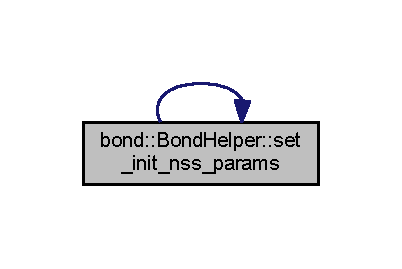
\includegraphics[width=193pt]{classbond_1_1_bond_helper_aaf31152498dbbf3704839a0c57e4555c_cgraph}
\end{center}
\end{figure}
Here is the caller graph for this function\+:
\nopagebreak
\begin{figure}[H]
\begin{center}
\leavevmode
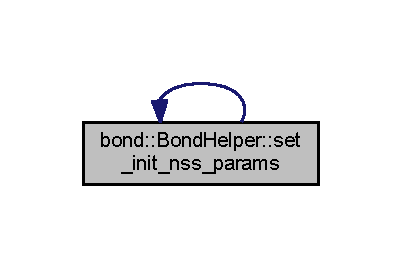
\includegraphics[width=193pt]{classbond_1_1_bond_helper_aaf31152498dbbf3704839a0c57e4555c_icgraph}
\end{center}
\end{figure}


\subsection{Member Data Documentation}
\mbox{\Hypertarget{classbond_1_1_bond_helper_a61db751f82d46ce2f7f5032ff2a3b03e}\label{classbond_1_1_bond_helper_a61db751f82d46ce2f7f5032ff2a3b03e}} 
\index{bond\+::\+Bond\+Helper@{bond\+::\+Bond\+Helper}!bonds@{bonds}}
\index{bonds@{bonds}!bond\+::\+Bond\+Helper@{bond\+::\+Bond\+Helper}}
\subsubsection{\texorpdfstring{bonds}{bonds}}
{\footnotesize\ttfamily template$<$typename T $>$ \\
std\+::vector$<$\hyperlink{classbond_1_1_bond}{Bond}$<$T$>$ $>$ \hyperlink{classbond_1_1_bond_helper}{bond\+::\+Bond\+Helper}$<$ T $>$\+::bonds\hspace{0.3cm}{\ttfamily [private]}}



Vector of bonds. 



Definition at line 93 of file bondhelper.\+h.

\mbox{\Hypertarget{classbond_1_1_bond_helper_a843e3c12a561aaac047ba70310375a2f}\label{classbond_1_1_bond_helper_a843e3c12a561aaac047ba70310375a2f}} 
\index{bond\+::\+Bond\+Helper@{bond\+::\+Bond\+Helper}!df\+\_\+type@{df\+\_\+type}}
\index{df\+\_\+type@{df\+\_\+type}!bond\+::\+Bond\+Helper@{bond\+::\+Bond\+Helper}}
\subsubsection{\texorpdfstring{df\+\_\+type}{df\_type}}
{\footnotesize\ttfamily template$<$typename T $>$ \\
const \hyperlink{namespaceutilities_ad4290e607d0651ce53db6e5c776aca7c}{D\+F\+\_\+type} \hyperlink{classbond_1_1_bond_helper}{bond\+::\+Bond\+Helper}$<$ T $>$\+::df\+\_\+type\hspace{0.3cm}{\ttfamily [private]}}



Discount Factor type. 



Definition at line 95 of file bondhelper.\+h.



The documentation for this class was generated from the following files\+:\begin{DoxyCompactItemize}
\item 
\hyperlink{bond_8h}{bond.\+h}\item 
\hyperlink{bondhelper_8h}{bondhelper.\+h}\end{DoxyCompactItemize}

\hypertarget{structea_1_1_d_e}{}\section{ea\+:\+:DE$<$ T $>$ Struct Template Reference}
\label{structea_1_1_d_e}\index{ea\+::\+D\+E$<$ T $>$@{ea\+::\+D\+E$<$ T $>$}}


Differential Evolution Structure, used in the actual algorithm and for type deduction.  




{\ttfamily \#include $<$differentialevo.\+h$>$}



Inheritance diagram for ea\+:\+:DE$<$ T $>$\+:
\nopagebreak
\begin{figure}[H]
\begin{center}
\leavevmode
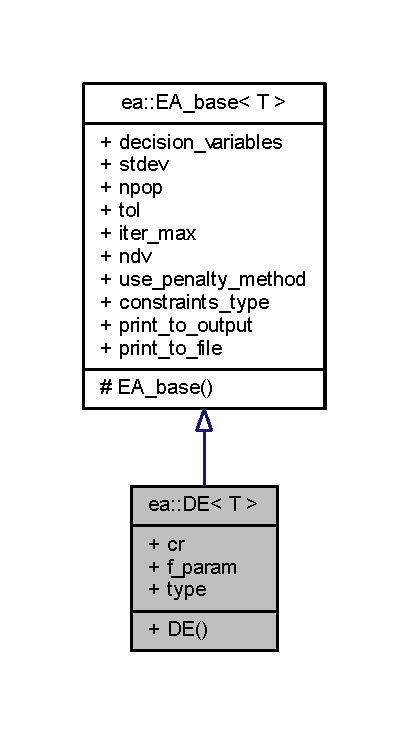
\includegraphics[width=196pt]{structea_1_1_d_e__inherit__graph}
\end{center}
\end{figure}
\subsection*{Public Member Functions}
\begin{DoxyCompactItemize}
\item 
\hyperlink{structea_1_1_d_e_a407d0c61464c79e200906e95370f70c4}{DE} (const T \&i\+\_\+cr, const T \&i\+\_\+f\+\_\+param, const std\+::vector$<$ T $>$ \&i\+\_\+decision\+\_\+variables, const std\+::vector$<$ T $>$ \&i\+\_\+stdev, const size\+\_\+t \&i\+\_\+npop, const T \&i\+\_\+tol, const size\+\_\+t \&i\+\_\+iter\+\_\+max, const bool \&i\+\_\+use\+\_\+penalty\+\_\+method, const \hyperlink{namespaceutilities_ab1a1517bf6e62a1acfab5293ca8985c1}{Constraints\+\_\+type} \&i\+\_\+constraints\+\_\+type, const bool \&i\+\_\+print\+\_\+to\+\_\+output, const bool \&i\+\_\+print\+\_\+to\+\_\+file)
\begin{DoxyCompactList}\small\item\em Constructor. \end{DoxyCompactList}\end{DoxyCompactItemize}
\subsection*{Public Attributes}
\begin{DoxyCompactItemize}
\item 
const T \hyperlink{structea_1_1_d_e_adc00ae4bfe7fb6c2581e08ca47e753b2}{cr}
\begin{DoxyCompactList}\small\item\em Crossover Rate. \end{DoxyCompactList}\item 
const T \hyperlink{structea_1_1_d_e_a6b798f4a095796b766b2452aacea8a6b}{f\+\_\+param}
\begin{DoxyCompactList}\small\item\em Mutation Scale Fuctor. \end{DoxyCompactList}\item 
const std\+::string \hyperlink{structea_1_1_d_e_a0968311419d1919244af4415b294739a}{type} = \char`\"{}Differential Evolution\char`\"{}
\begin{DoxyCompactList}\small\item\em Type of the algorithm. \end{DoxyCompactList}\end{DoxyCompactItemize}
\subsection*{Additional Inherited Members}


\subsection{Detailed Description}
\subsubsection*{template$<$typename T$>$\newline
struct ea\+::\+D\+E$<$ T $>$}

Differential Evolution Structure, used in the actual algorithm and for type deduction. 

Definition at line 16 of file differentialevo.\+h.



\subsection{Constructor \& Destructor Documentation}
\mbox{\Hypertarget{structea_1_1_d_e_a407d0c61464c79e200906e95370f70c4}\label{structea_1_1_d_e_a407d0c61464c79e200906e95370f70c4}} 
\index{ea\+::\+DE@{ea\+::\+DE}!DE@{DE}}
\index{DE@{DE}!ea\+::\+DE@{ea\+::\+DE}}
\subsubsection{\texorpdfstring{D\+E()}{DE()}}
{\footnotesize\ttfamily template$<$typename T$>$ \\
\hyperlink{structea_1_1_d_e}{ea\+::\+DE}$<$ T $>$\+::\hyperlink{structea_1_1_d_e}{DE} (\begin{DoxyParamCaption}\item[{const T \&}]{i\+\_\+cr,  }\item[{const T \&}]{i\+\_\+f\+\_\+param,  }\item[{const std\+::vector$<$ T $>$ \&}]{i\+\_\+decision\+\_\+variables,  }\item[{const std\+::vector$<$ T $>$ \&}]{i\+\_\+stdev,  }\item[{const size\+\_\+t \&}]{i\+\_\+npop,  }\item[{const T \&}]{i\+\_\+tol,  }\item[{const size\+\_\+t \&}]{i\+\_\+iter\+\_\+max,  }\item[{const bool \&}]{i\+\_\+use\+\_\+penalty\+\_\+method = {\ttfamily false},  }\item[{const \hyperlink{namespaceutilities_ab1a1517bf6e62a1acfab5293ca8985c1}{Constraints\+\_\+type} \&}]{i\+\_\+constraints\+\_\+type = {\ttfamily \hyperlink{namespaceea_a8e369877773b4db67b8512efdb4f8f89a334c4a4c42fdb79d7ebc3e73b517e6f8}{Constraints\+\_\+type\+::none}},  }\item[{const bool \&}]{i\+\_\+print\+\_\+to\+\_\+output = {\ttfamily true},  }\item[{const bool \&}]{i\+\_\+print\+\_\+to\+\_\+file = {\ttfamily true} }\end{DoxyParamCaption})\hspace{0.3cm}{\ttfamily [inline]}}



Constructor. 


\begin{DoxyParams}{Parameters}
{\em i\+\_\+cr} & Crossover Rate \\
\hline
{\em i\+\_\+f\+\_\+param} & Mutation Scale Factor \\
\hline
{\em i\+\_\+decision\+\_\+variables} & The starting values of the decision variables \\
\hline
{\em i\+\_\+stdev} & The standard deviation \\
\hline
{\em i\+\_\+npop} & The population size \\
\hline
{\em i\+\_\+tol} & The tolerance \\
\hline
{\em i\+\_\+iter\+\_\+max} & The maximum number of iterations \\
\hline
{\em i\+\_\+use\+\_\+penalty\+\_\+method} & Whether to used penalties or not \\
\hline
{\em i\+\_\+constraints\+\_\+type} & What kind of constraints to use \\
\hline
{\em i\+\_\+print\+\_\+to\+\_\+output} & Whether to print to terminal or not \\
\hline
{\em i\+\_\+print\+\_\+to\+\_\+file} & Whether to print to a file or not \\
\hline
\end{DoxyParams}
\begin{DoxyReturn}{Returns}
A D\+E$<$\+T$>$ object 
\end{DoxyReturn}


Definition at line 37 of file differentialevo.\+h.



References ea\+::\+D\+E$<$ T $>$\+::cr, and ea\+::\+D\+E$<$ T $>$\+::f\+\_\+param.


\begin{DoxyCode}
40                                                                         :
41             EA\_base<T>(i\_decision\_variables, i\_stdev, i\_npop, i\_tol, i\_iter\_max, i\_use\_penalty\_method, 
      i\_constraints\_type, i\_print\_to\_output, i\_print\_to\_file),
42             \hyperlink{structea_1_1_d_e_adc00ae4bfe7fb6c2581e08ca47e753b2}{cr}( i\_cr ),
43             \hyperlink{structea_1_1_d_e_a6b798f4a095796b766b2452aacea8a6b}{f\_param}( i\_f\_param )
44         \{
45             assert(\hyperlink{structea_1_1_d_e_adc00ae4bfe7fb6c2581e08ca47e753b2}{cr} > 0 && \hyperlink{structea_1_1_d_e_adc00ae4bfe7fb6c2581e08ca47e753b2}{cr} <= 1);
46             assert(\hyperlink{structea_1_1_d_e_a6b798f4a095796b766b2452aacea8a6b}{f\_param} > 0 && \hyperlink{structea_1_1_d_e_a6b798f4a095796b766b2452aacea8a6b}{f\_param} <= 1);
47         \}
\end{DoxyCode}


\subsection{Member Data Documentation}
\mbox{\Hypertarget{structea_1_1_d_e_adc00ae4bfe7fb6c2581e08ca47e753b2}\label{structea_1_1_d_e_adc00ae4bfe7fb6c2581e08ca47e753b2}} 
\index{ea\+::\+DE@{ea\+::\+DE}!cr@{cr}}
\index{cr@{cr}!ea\+::\+DE@{ea\+::\+DE}}
\subsubsection{\texorpdfstring{cr}{cr}}
{\footnotesize\ttfamily template$<$typename T$>$ \\
const T \hyperlink{structea_1_1_d_e}{ea\+::\+DE}$<$ T $>$\+::cr}



Crossover Rate. 



Definition at line 49 of file differentialevo.\+h.



Referenced by ea\+::\+D\+E$<$ T $>$\+::\+D\+E(), and ea\+::\+Solver$<$ D\+E, T, F, C $>$\+::display\+\_\+parameters().

\mbox{\Hypertarget{structea_1_1_d_e_a6b798f4a095796b766b2452aacea8a6b}\label{structea_1_1_d_e_a6b798f4a095796b766b2452aacea8a6b}} 
\index{ea\+::\+DE@{ea\+::\+DE}!f\+\_\+param@{f\+\_\+param}}
\index{f\+\_\+param@{f\+\_\+param}!ea\+::\+DE@{ea\+::\+DE}}
\subsubsection{\texorpdfstring{f\+\_\+param}{f\_param}}
{\footnotesize\ttfamily template$<$typename T$>$ \\
const T \hyperlink{structea_1_1_d_e}{ea\+::\+DE}$<$ T $>$\+::f\+\_\+param}



Mutation Scale Fuctor. 



Definition at line 51 of file differentialevo.\+h.



Referenced by ea\+::\+D\+E$<$ T $>$\+::\+D\+E(), and ea\+::\+Solver$<$ D\+E, T, F, C $>$\+::display\+\_\+parameters().

\mbox{\Hypertarget{structea_1_1_d_e_a0968311419d1919244af4415b294739a}\label{structea_1_1_d_e_a0968311419d1919244af4415b294739a}} 
\index{ea\+::\+DE@{ea\+::\+DE}!type@{type}}
\index{type@{type}!ea\+::\+DE@{ea\+::\+DE}}
\subsubsection{\texorpdfstring{type}{type}}
{\footnotesize\ttfamily template$<$typename T$>$ \\
const std\+::string \hyperlink{structea_1_1_d_e}{ea\+::\+DE}$<$ T $>$\+::type = \char`\"{}Differential Evolution\char`\"{}}



Type of the algorithm. 



Definition at line 53 of file differentialevo.\+h.



The documentation for this struct was generated from the following file\+:\begin{DoxyCompactItemize}
\item 
\hyperlink{differentialevo_8h}{differentialevo.\+h}\end{DoxyCompactItemize}

\hypertarget{structea_1_1_e_a__base}{}\section{ea\+:\+:E\+A\+\_\+base$<$ T $>$ Struct Template Reference}
\label{structea_1_1_e_a__base}\index{ea\+::\+E\+A\+\_\+base$<$ T $>$@{ea\+::\+E\+A\+\_\+base$<$ T $>$}}


Evolutionary algorithm stucture base.  




{\ttfamily \#include $<$ealgorithm\+\_\+base.\+h$>$}



Inheritance diagram for ea\+:\+:E\+A\+\_\+base$<$ T $>$\+:
\nopagebreak
\begin{figure}[H]
\begin{center}
\leavevmode
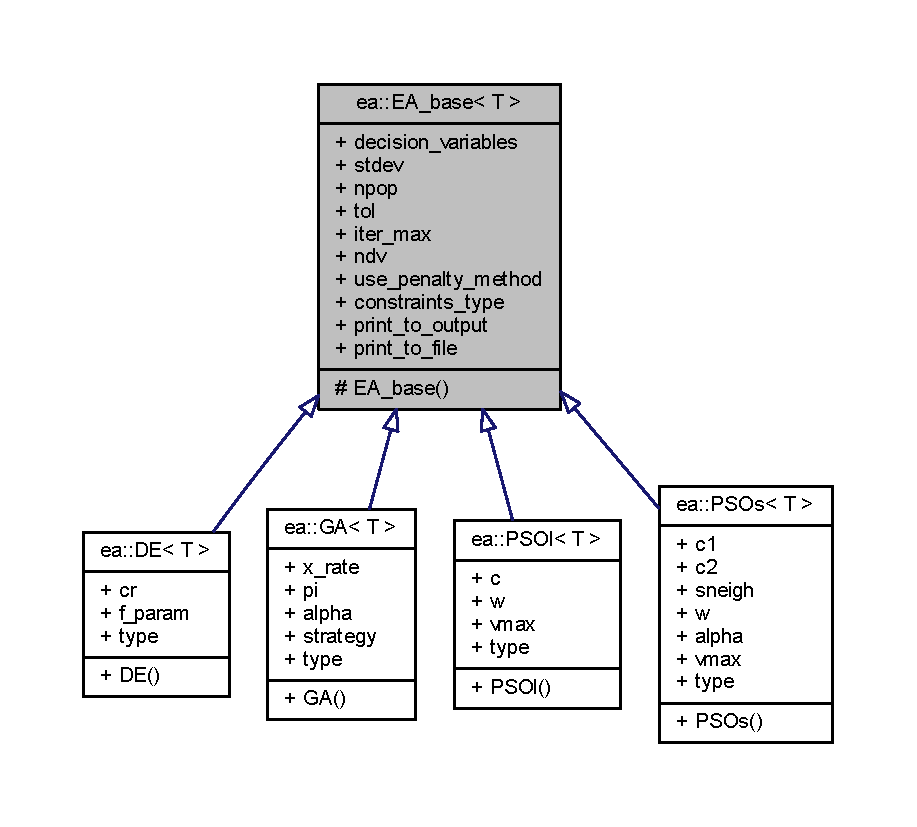
\includegraphics[width=350pt]{structea_1_1_e_a__base__inherit__graph}
\end{center}
\end{figure}
\subsection*{Public Types}
\begin{DoxyCompactItemize}
\item 
using \hyperlink{structea_1_1_e_a__base_ab626cb28104f750a38092a742c9fa996}{fp\+\_\+type} = T
\begin{DoxyCompactList}\small\item\em The floating point number type used for type deduction. \end{DoxyCompactList}\end{DoxyCompactItemize}
\subsection*{Public Attributes}
\begin{DoxyCompactItemize}
\item 
const std\+::vector$<$ T $>$ \hyperlink{structea_1_1_e_a__base_a71e09437e78efc6e93e0a6e510d13100}{decision\+\_\+variables}
\begin{DoxyCompactList}\small\item\em Initial Decision Variables. \end{DoxyCompactList}\item 
const std\+::vector$<$ T $>$ \hyperlink{structea_1_1_e_a__base_a28216728d1e1355337d8bf2a484d5569}{stdev}
\begin{DoxyCompactList}\small\item\em Standard deviation of the decision variables. \end{DoxyCompactList}\item 
const size\+\_\+t \hyperlink{structea_1_1_e_a__base_a41b6ed30e866d5f6a782a90e6a1b0f79}{npop}
\begin{DoxyCompactList}\small\item\em Size of the population. \end{DoxyCompactList}\item 
const T \hyperlink{structea_1_1_e_a__base_a9b7a33797adc1cbeab7a9f3786c41a27}{tol}
\begin{DoxyCompactList}\small\item\em Tolerance. \end{DoxyCompactList}\item 
const size\+\_\+t \hyperlink{structea_1_1_e_a__base_affe85fad1da440e091a9d09cf46d502f}{iter\+\_\+max}
\begin{DoxyCompactList}\small\item\em Number of maximum iterations. \end{DoxyCompactList}\item 
const size\+\_\+t \hyperlink{structea_1_1_e_a__base_a6996abed1c0b9642bdae67547fa6474c}{ndv}
\begin{DoxyCompactList}\small\item\em Number of decision variables. \end{DoxyCompactList}\item 
const bool \hyperlink{structea_1_1_e_a__base_ad3b4a962208b72c67b663ba0d40bebfb}{use\+\_\+penalty\+\_\+method}
\begin{DoxyCompactList}\small\item\em Use penalty function or not. \end{DoxyCompactList}\item 
const \hyperlink{namespaceutilities_ab1a1517bf6e62a1acfab5293ca8985c1}{Constraints\+\_\+type} \hyperlink{structea_1_1_e_a__base_a8f6f21a54d24fa69833cfd1a59beeed3}{constraints\+\_\+type}
\begin{DoxyCompactList}\small\item\em Constraints type. \end{DoxyCompactList}\item 
const bool \hyperlink{structea_1_1_e_a__base_aea758485e2120469ca02c52c7cff9e5a}{print\+\_\+to\+\_\+output}
\begin{DoxyCompactList}\small\item\em Print to output or not. \end{DoxyCompactList}\item 
const bool \hyperlink{structea_1_1_e_a__base_a9ad71465eab92ffd0fe98b625d2d15bc}{print\+\_\+to\+\_\+file}
\begin{DoxyCompactList}\small\item\em Print to file or not. \end{DoxyCompactList}\end{DoxyCompactItemize}
\subsection*{Protected Member Functions}
\begin{DoxyCompactItemize}
\item 
\hyperlink{structea_1_1_e_a__base_a4dd8bb67732d28ba3d084ddcd6ee1858}{E\+A\+\_\+base} (const std\+::vector$<$ T $>$ \&i\+\_\+decision\+\_\+variables, const std\+::vector$<$ T $>$ \&i\+\_\+stdev, const size\+\_\+t \&i\+\_\+npop, const T \&i\+\_\+tol, const size\+\_\+t \&i\+\_\+iter\+\_\+max, const bool \&i\+\_\+use\+\_\+penalty\+\_\+method, const \hyperlink{namespaceutilities_ab1a1517bf6e62a1acfab5293ca8985c1}{Constraints\+\_\+type} \&i\+\_\+constraints\+\_\+type, const bool \&i\+\_\+print\+\_\+to\+\_\+output, const bool \&i\+\_\+print\+\_\+to\+\_\+file)
\begin{DoxyCompactList}\small\item\em Constructor. \end{DoxyCompactList}\end{DoxyCompactItemize}


\subsection{Detailed Description}
\subsubsection*{template$<$typename T$>$\newline
struct ea\+::\+E\+A\+\_\+base$<$ T $>$}

Evolutionary algorithm stucture base. 

Definition at line 28 of file ealgorithm\+\_\+base.\+h.



\subsection{Member Typedef Documentation}
\mbox{\Hypertarget{structea_1_1_e_a__base_ab626cb28104f750a38092a742c9fa996}\label{structea_1_1_e_a__base_ab626cb28104f750a38092a742c9fa996}} 
\index{ea\+::\+E\+A\+\_\+base@{ea\+::\+E\+A\+\_\+base}!fp\+\_\+type@{fp\+\_\+type}}
\index{fp\+\_\+type@{fp\+\_\+type}!ea\+::\+E\+A\+\_\+base@{ea\+::\+E\+A\+\_\+base}}
\subsubsection{\texorpdfstring{fp\+\_\+type}{fp\_type}}
{\footnotesize\ttfamily template$<$typename T $>$ \\
using \hyperlink{structea_1_1_e_a__base}{ea\+::\+E\+A\+\_\+base}$<$ T $>$\+::\hyperlink{structea_1_1_e_a__base_ab626cb28104f750a38092a742c9fa996}{fp\+\_\+type} =  T}



The floating point number type used for type deduction. 



Definition at line 32 of file ealgorithm\+\_\+base.\+h.



\subsection{Constructor \& Destructor Documentation}
\mbox{\Hypertarget{structea_1_1_e_a__base_a4dd8bb67732d28ba3d084ddcd6ee1858}\label{structea_1_1_e_a__base_a4dd8bb67732d28ba3d084ddcd6ee1858}} 
\index{ea\+::\+E\+A\+\_\+base@{ea\+::\+E\+A\+\_\+base}!E\+A\+\_\+base@{E\+A\+\_\+base}}
\index{E\+A\+\_\+base@{E\+A\+\_\+base}!ea\+::\+E\+A\+\_\+base@{ea\+::\+E\+A\+\_\+base}}
\subsubsection{\texorpdfstring{E\+A\+\_\+base()}{EA\_base()}}
{\footnotesize\ttfamily template$<$typename T $>$ \\
\hyperlink{structea_1_1_e_a__base}{ea\+::\+E\+A\+\_\+base}$<$ T $>$\+::\hyperlink{structea_1_1_e_a__base}{E\+A\+\_\+base} (\begin{DoxyParamCaption}\item[{const std\+::vector$<$ T $>$ \&}]{i\+\_\+decision\+\_\+variables,  }\item[{const std\+::vector$<$ T $>$ \&}]{i\+\_\+stdev,  }\item[{const size\+\_\+t \&}]{i\+\_\+npop,  }\item[{const T \&}]{i\+\_\+tol,  }\item[{const size\+\_\+t \&}]{i\+\_\+iter\+\_\+max,  }\item[{const bool \&}]{i\+\_\+use\+\_\+penalty\+\_\+method,  }\item[{const \hyperlink{namespaceutilities_ab1a1517bf6e62a1acfab5293ca8985c1}{Constraints\+\_\+type} \&}]{i\+\_\+constraints\+\_\+type,  }\item[{const bool \&}]{i\+\_\+print\+\_\+to\+\_\+output,  }\item[{const bool \&}]{i\+\_\+print\+\_\+to\+\_\+file }\end{DoxyParamCaption})\hspace{0.3cm}{\ttfamily [inline]}, {\ttfamily [protected]}}



Constructor. 


\begin{DoxyParams}{Parameters}
{\em i\+\_\+decision\+\_\+variables} & The starting values of the decision variables \\
\hline
{\em i\+\_\+stdev} & The standard deviation \\
\hline
{\em i\+\_\+npop} & The population size \\
\hline
{\em i\+\_\+tol} & The tolerance \\
\hline
{\em i\+\_\+iter\+\_\+max} & The maximum number of iterations \\
\hline
{\em i\+\_\+use\+\_\+penalty\+\_\+method} & Whether to used penalties or not \\
\hline
{\em i\+\_\+constraints\+\_\+type} & What kind of constraints to use \\
\hline
{\em i\+\_\+print\+\_\+to\+\_\+output} & Whether to print to terminal or not \\
\hline
{\em i\+\_\+print\+\_\+to\+\_\+file} & Whether to print to a file or not \\
\hline
\end{DoxyParams}
\begin{DoxyReturn}{Returns}
A E\+A\+\_\+base$<$\+T$>$ object 
\end{DoxyReturn}


Definition at line 68 of file ealgorithm\+\_\+base.\+h.


\begin{DoxyCode}
70             : \hyperlink{structea_1_1_e_a__base_a71e09437e78efc6e93e0a6e510d13100}{decision\_variables}\{ i\_decision\_variables \}, 
      \hyperlink{structea_1_1_e_a__base_a28216728d1e1355337d8bf2a484d5569}{stdev}\{ i\_stdev \}, \hyperlink{structea_1_1_e_a__base_a41b6ed30e866d5f6a782a90e6a1b0f79}{npop}\{ i\_npop \}, \hyperlink{structea_1_1_e_a__base_a9b7a33797adc1cbeab7a9f3786c41a27}{tol}\{ i\_tol \}, \hyperlink{structea_1_1_e_a__base_affe85fad1da440e091a9d09cf46d502f}{iter\_max}\{ i\_iter\_max \}, 
      \hyperlink{structea_1_1_e_a__base_a6996abed1c0b9642bdae67547fa6474c}{ndv}\{ i\_decision\_variables.size() \},
71             \hyperlink{structea_1_1_e_a__base_ad3b4a962208b72c67b663ba0d40bebfb}{use\_penalty\_method}\{ i\_use\_penalty\_method \}, 
      \hyperlink{structea_1_1_e_a__base_a8f6f21a54d24fa69833cfd1a59beeed3}{constraints\_type}\{ i\_constraints\_type \}, \hyperlink{structea_1_1_e_a__base_aea758485e2120469ca02c52c7cff9e5a}{print\_to\_output}\{ i\_print\_to\_output \}
      , \hyperlink{structea_1_1_e_a__base_a9ad71465eab92ffd0fe98b625d2d15bc}{print\_to\_file}\{ i\_print\_to\_file \}
72         \{
73             assert(\hyperlink{structea_1_1_e_a__base_a71e09437e78efc6e93e0a6e510d13100}{decision\_variables}.size() > 0);
74             assert(\hyperlink{structea_1_1_e_a__base_a71e09437e78efc6e93e0a6e510d13100}{decision\_variables}.size() == \hyperlink{structea_1_1_e_a__base_a28216728d1e1355337d8bf2a484d5569}{stdev}.size());
75             \textcolor{keywordflow}{for} (\textcolor{keyword}{const} \textcolor{keyword}{auto}& p : \hyperlink{structea_1_1_e_a__base_a28216728d1e1355337d8bf2a484d5569}{stdev})
76             \{
77                 assert(p > 0);
78             \}
79             assert(\hyperlink{structea_1_1_e_a__base_a41b6ed30e866d5f6a782a90e6a1b0f79}{npop} > 0);
80             assert(\hyperlink{structea_1_1_e_a__base_a9b7a33797adc1cbeab7a9f3786c41a27}{tol} > 0);
81             assert(\hyperlink{structea_1_1_e_a__base_affe85fad1da440e091a9d09cf46d502f}{iter\_max} > 0);
82         \}
\end{DoxyCode}


\subsection{Member Data Documentation}
\mbox{\Hypertarget{structea_1_1_e_a__base_a8f6f21a54d24fa69833cfd1a59beeed3}\label{structea_1_1_e_a__base_a8f6f21a54d24fa69833cfd1a59beeed3}} 
\index{ea\+::\+E\+A\+\_\+base@{ea\+::\+E\+A\+\_\+base}!constraints\+\_\+type@{constraints\+\_\+type}}
\index{constraints\+\_\+type@{constraints\+\_\+type}!ea\+::\+E\+A\+\_\+base@{ea\+::\+E\+A\+\_\+base}}
\subsubsection{\texorpdfstring{constraints\+\_\+type}{constraints\_type}}
{\footnotesize\ttfamily template$<$typename T $>$ \\
const \hyperlink{namespaceutilities_ab1a1517bf6e62a1acfab5293ca8985c1}{Constraints\+\_\+type} \hyperlink{structea_1_1_e_a__base}{ea\+::\+E\+A\+\_\+base}$<$ T $>$\+::constraints\+\_\+type}



Constraints type. 



Definition at line 48 of file ealgorithm\+\_\+base.\+h.

\mbox{\Hypertarget{structea_1_1_e_a__base_a71e09437e78efc6e93e0a6e510d13100}\label{structea_1_1_e_a__base_a71e09437e78efc6e93e0a6e510d13100}} 
\index{ea\+::\+E\+A\+\_\+base@{ea\+::\+E\+A\+\_\+base}!decision\+\_\+variables@{decision\+\_\+variables}}
\index{decision\+\_\+variables@{decision\+\_\+variables}!ea\+::\+E\+A\+\_\+base@{ea\+::\+E\+A\+\_\+base}}
\subsubsection{\texorpdfstring{decision\+\_\+variables}{decision\_variables}}
{\footnotesize\ttfamily template$<$typename T $>$ \\
const std\+::vector$<$T$>$ \hyperlink{structea_1_1_e_a__base}{ea\+::\+E\+A\+\_\+base}$<$ T $>$\+::decision\+\_\+variables}



Initial Decision Variables. 



Definition at line 34 of file ealgorithm\+\_\+base.\+h.

\mbox{\Hypertarget{structea_1_1_e_a__base_affe85fad1da440e091a9d09cf46d502f}\label{structea_1_1_e_a__base_affe85fad1da440e091a9d09cf46d502f}} 
\index{ea\+::\+E\+A\+\_\+base@{ea\+::\+E\+A\+\_\+base}!iter\+\_\+max@{iter\+\_\+max}}
\index{iter\+\_\+max@{iter\+\_\+max}!ea\+::\+E\+A\+\_\+base@{ea\+::\+E\+A\+\_\+base}}
\subsubsection{\texorpdfstring{iter\+\_\+max}{iter\_max}}
{\footnotesize\ttfamily template$<$typename T $>$ \\
const size\+\_\+t \hyperlink{structea_1_1_e_a__base}{ea\+::\+E\+A\+\_\+base}$<$ T $>$\+::iter\+\_\+max}



Number of maximum iterations. 



Definition at line 42 of file ealgorithm\+\_\+base.\+h.

\mbox{\Hypertarget{structea_1_1_e_a__base_a6996abed1c0b9642bdae67547fa6474c}\label{structea_1_1_e_a__base_a6996abed1c0b9642bdae67547fa6474c}} 
\index{ea\+::\+E\+A\+\_\+base@{ea\+::\+E\+A\+\_\+base}!ndv@{ndv}}
\index{ndv@{ndv}!ea\+::\+E\+A\+\_\+base@{ea\+::\+E\+A\+\_\+base}}
\subsubsection{\texorpdfstring{ndv}{ndv}}
{\footnotesize\ttfamily template$<$typename T $>$ \\
const size\+\_\+t \hyperlink{structea_1_1_e_a__base}{ea\+::\+E\+A\+\_\+base}$<$ T $>$\+::ndv}



Number of decision variables. 



Definition at line 44 of file ealgorithm\+\_\+base.\+h.



Referenced by ea\+::\+P\+S\+Ol$<$ T $>$\+::\+P\+S\+Ol(), and ea\+::\+P\+S\+Os$<$ T $>$\+::\+P\+S\+Os().

\mbox{\Hypertarget{structea_1_1_e_a__base_a41b6ed30e866d5f6a782a90e6a1b0f79}\label{structea_1_1_e_a__base_a41b6ed30e866d5f6a782a90e6a1b0f79}} 
\index{ea\+::\+E\+A\+\_\+base@{ea\+::\+E\+A\+\_\+base}!npop@{npop}}
\index{npop@{npop}!ea\+::\+E\+A\+\_\+base@{ea\+::\+E\+A\+\_\+base}}
\subsubsection{\texorpdfstring{npop}{npop}}
{\footnotesize\ttfamily template$<$typename T $>$ \\
const size\+\_\+t \hyperlink{structea_1_1_e_a__base}{ea\+::\+E\+A\+\_\+base}$<$ T $>$\+::npop}



Size of the population. 



Definition at line 38 of file ealgorithm\+\_\+base.\+h.



Referenced by ea\+::\+Solver$<$ D\+E, T, F, C $>$\+::set\+\_\+indices().

\mbox{\Hypertarget{structea_1_1_e_a__base_a9ad71465eab92ffd0fe98b625d2d15bc}\label{structea_1_1_e_a__base_a9ad71465eab92ffd0fe98b625d2d15bc}} 
\index{ea\+::\+E\+A\+\_\+base@{ea\+::\+E\+A\+\_\+base}!print\+\_\+to\+\_\+file@{print\+\_\+to\+\_\+file}}
\index{print\+\_\+to\+\_\+file@{print\+\_\+to\+\_\+file}!ea\+::\+E\+A\+\_\+base@{ea\+::\+E\+A\+\_\+base}}
\subsubsection{\texorpdfstring{print\+\_\+to\+\_\+file}{print\_to\_file}}
{\footnotesize\ttfamily template$<$typename T $>$ \\
const bool \hyperlink{structea_1_1_e_a__base}{ea\+::\+E\+A\+\_\+base}$<$ T $>$\+::print\+\_\+to\+\_\+file}



Print to file or not. 



Definition at line 52 of file ealgorithm\+\_\+base.\+h.

\mbox{\Hypertarget{structea_1_1_e_a__base_aea758485e2120469ca02c52c7cff9e5a}\label{structea_1_1_e_a__base_aea758485e2120469ca02c52c7cff9e5a}} 
\index{ea\+::\+E\+A\+\_\+base@{ea\+::\+E\+A\+\_\+base}!print\+\_\+to\+\_\+output@{print\+\_\+to\+\_\+output}}
\index{print\+\_\+to\+\_\+output@{print\+\_\+to\+\_\+output}!ea\+::\+E\+A\+\_\+base@{ea\+::\+E\+A\+\_\+base}}
\subsubsection{\texorpdfstring{print\+\_\+to\+\_\+output}{print\_to\_output}}
{\footnotesize\ttfamily template$<$typename T $>$ \\
const bool \hyperlink{structea_1_1_e_a__base}{ea\+::\+E\+A\+\_\+base}$<$ T $>$\+::print\+\_\+to\+\_\+output}



Print to output or not. 



Definition at line 50 of file ealgorithm\+\_\+base.\+h.

\mbox{\Hypertarget{structea_1_1_e_a__base_a28216728d1e1355337d8bf2a484d5569}\label{structea_1_1_e_a__base_a28216728d1e1355337d8bf2a484d5569}} 
\index{ea\+::\+E\+A\+\_\+base@{ea\+::\+E\+A\+\_\+base}!stdev@{stdev}}
\index{stdev@{stdev}!ea\+::\+E\+A\+\_\+base@{ea\+::\+E\+A\+\_\+base}}
\subsubsection{\texorpdfstring{stdev}{stdev}}
{\footnotesize\ttfamily template$<$typename T $>$ \\
const std\+::vector$<$T$>$ \hyperlink{structea_1_1_e_a__base}{ea\+::\+E\+A\+\_\+base}$<$ T $>$\+::stdev}



Standard deviation of the decision variables. 



Definition at line 36 of file ealgorithm\+\_\+base.\+h.

\mbox{\Hypertarget{structea_1_1_e_a__base_a9b7a33797adc1cbeab7a9f3786c41a27}\label{structea_1_1_e_a__base_a9b7a33797adc1cbeab7a9f3786c41a27}} 
\index{ea\+::\+E\+A\+\_\+base@{ea\+::\+E\+A\+\_\+base}!tol@{tol}}
\index{tol@{tol}!ea\+::\+E\+A\+\_\+base@{ea\+::\+E\+A\+\_\+base}}
\subsubsection{\texorpdfstring{tol}{tol}}
{\footnotesize\ttfamily template$<$typename T $>$ \\
const T \hyperlink{structea_1_1_e_a__base}{ea\+::\+E\+A\+\_\+base}$<$ T $>$\+::tol}



Tolerance. 



Definition at line 40 of file ealgorithm\+\_\+base.\+h.

\mbox{\Hypertarget{structea_1_1_e_a__base_ad3b4a962208b72c67b663ba0d40bebfb}\label{structea_1_1_e_a__base_ad3b4a962208b72c67b663ba0d40bebfb}} 
\index{ea\+::\+E\+A\+\_\+base@{ea\+::\+E\+A\+\_\+base}!use\+\_\+penalty\+\_\+method@{use\+\_\+penalty\+\_\+method}}
\index{use\+\_\+penalty\+\_\+method@{use\+\_\+penalty\+\_\+method}!ea\+::\+E\+A\+\_\+base@{ea\+::\+E\+A\+\_\+base}}
\subsubsection{\texorpdfstring{use\+\_\+penalty\+\_\+method}{use\_penalty\_method}}
{\footnotesize\ttfamily template$<$typename T $>$ \\
const bool \hyperlink{structea_1_1_e_a__base}{ea\+::\+E\+A\+\_\+base}$<$ T $>$\+::use\+\_\+penalty\+\_\+method}



Use penalty function or not. 



Definition at line 46 of file ealgorithm\+\_\+base.\+h.



The documentation for this struct was generated from the following file\+:\begin{DoxyCompactItemize}
\item 
\hyperlink{ealgorithm__base_8h}{ealgorithm\+\_\+base.\+h}\end{DoxyCompactItemize}

\hypertarget{structea_1_1_g_a}{}\section{ea\+:\+:GA$<$ T $>$ Struct Template Reference}
\label{structea_1_1_g_a}\index{ea\+::\+G\+A$<$ T $>$@{ea\+::\+G\+A$<$ T $>$}}


Genetic Algorithms Structure, used in the actual algorithm and for type deduction.  




{\ttfamily \#include $<$geneticalgo.\+h$>$}



Inheritance diagram for ea\+:\+:GA$<$ T $>$\+:
\nopagebreak
\begin{figure}[H]
\begin{center}
\leavevmode
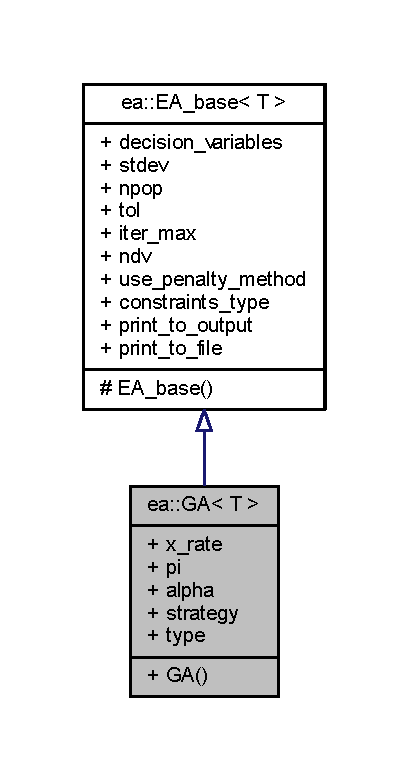
\includegraphics[width=196pt]{structea_1_1_g_a__inherit__graph}
\end{center}
\end{figure}
\subsection*{Public Member Functions}
\begin{DoxyCompactItemize}
\item 
\hyperlink{structea_1_1_g_a_a5a8abc8d099a169a0c141079552be2c3}{GA} (const T \&i\+\_\+x\+\_\+rate, const T \&i\+\_\+pi, const T \&i\+\_\+alpha, const std\+::vector$<$ T $>$ \&i\+\_\+decision\+\_\+variables, const std\+::vector$<$ T $>$ \&i\+\_\+stdev, const size\+\_\+t \&i\+\_\+npop, const T \&i\+\_\+tol, const size\+\_\+t \&i\+\_\+iter\+\_\+max, const bool \&i\+\_\+use\+\_\+penalty\+\_\+method, const \hyperlink{namespaceutilities_ab1a1517bf6e62a1acfab5293ca8985c1}{Constraints\+\_\+type} \&i\+\_\+constraints\+\_\+type, const \hyperlink{namespaceea_a8e369877773b4db67b8512efdb4f8f89}{Strategy} \&i\+\_\+strategy, const bool \&i\+\_\+print\+\_\+to\+\_\+output, const bool \&i\+\_\+print\+\_\+to\+\_\+file)
\begin{DoxyCompactList}\small\item\em Constructor. \end{DoxyCompactList}\end{DoxyCompactItemize}
\subsection*{Public Attributes}
\begin{DoxyCompactItemize}
\item 
const T \hyperlink{structea_1_1_g_a_ab72149b9ca39f385432e5310f4ae5ed6}{x\+\_\+rate}
\begin{DoxyCompactList}\small\item\em Natural Selection rate. \end{DoxyCompactList}\item 
const T \hyperlink{structea_1_1_g_a_a1efaa83a84ddebf8825308cdf2b7b2ce}{pi}
\begin{DoxyCompactList}\small\item\em Probability of mutating. \end{DoxyCompactList}\item 
const T \hyperlink{structea_1_1_g_a_a620f9573d21cc8eb9f49bfd8dc5086cc}{alpha}
\begin{DoxyCompactList}\small\item\em Parameter alpha for Beta distribution. \end{DoxyCompactList}\item 
const \hyperlink{namespaceea_a8e369877773b4db67b8512efdb4f8f89}{Strategy} \hyperlink{structea_1_1_g_a_a0bb275a7550304c1ae4c19db06ed8969}{strategy}
\begin{DoxyCompactList}\small\item\em Replacing or remove individuals strategies during mutation. \end{DoxyCompactList}\item 
const std\+::string \hyperlink{structea_1_1_g_a_a513eb50f77399d52e1aebf7d200b44c8}{type} = \char`\"{}Genetic Algorithms\char`\"{}
\begin{DoxyCompactList}\small\item\em Type of the algorithm. \end{DoxyCompactList}\end{DoxyCompactItemize}
\subsection*{Additional Inherited Members}


\subsection{Detailed Description}
\subsubsection*{template$<$typename T$>$\newline
struct ea\+::\+G\+A$<$ T $>$}

Genetic Algorithms Structure, used in the actual algorithm and for type deduction. 

Definition at line 21 of file geneticalgo.\+h.



\subsection{Constructor \& Destructor Documentation}
\mbox{\Hypertarget{structea_1_1_g_a_a5a8abc8d099a169a0c141079552be2c3}\label{structea_1_1_g_a_a5a8abc8d099a169a0c141079552be2c3}} 
\index{ea\+::\+GA@{ea\+::\+GA}!GA@{GA}}
\index{GA@{GA}!ea\+::\+GA@{ea\+::\+GA}}
\subsubsection{\texorpdfstring{G\+A()}{GA()}}
{\footnotesize\ttfamily template$<$typename T$>$ \\
\hyperlink{structea_1_1_g_a}{ea\+::\+GA}$<$ T $>$\+::\hyperlink{structea_1_1_g_a}{GA} (\begin{DoxyParamCaption}\item[{const T \&}]{i\+\_\+x\+\_\+rate,  }\item[{const T \&}]{i\+\_\+pi,  }\item[{const T \&}]{i\+\_\+alpha,  }\item[{const std\+::vector$<$ T $>$ \&}]{i\+\_\+decision\+\_\+variables,  }\item[{const std\+::vector$<$ T $>$ \&}]{i\+\_\+stdev,  }\item[{const size\+\_\+t \&}]{i\+\_\+npop,  }\item[{const T \&}]{i\+\_\+tol,  }\item[{const size\+\_\+t \&}]{i\+\_\+iter\+\_\+max,  }\item[{const bool \&}]{i\+\_\+use\+\_\+penalty\+\_\+method = {\ttfamily false},  }\item[{const \hyperlink{namespaceutilities_ab1a1517bf6e62a1acfab5293ca8985c1}{Constraints\+\_\+type} \&}]{i\+\_\+constraints\+\_\+type = {\ttfamily \hyperlink{namespaceea_a8e369877773b4db67b8512efdb4f8f89a334c4a4c42fdb79d7ebc3e73b517e6f8}{Constraints\+\_\+type\+::none}},  }\item[{const \hyperlink{namespaceea_a8e369877773b4db67b8512efdb4f8f89}{Strategy} \&}]{i\+\_\+strategy = {\ttfamily \hyperlink{namespaceea_a8e369877773b4db67b8512efdb4f8f89ac4a301043ce8554dfced7a0c0698bdad}{Strategy\+::keep\+\_\+same}},  }\item[{const bool \&}]{i\+\_\+print\+\_\+to\+\_\+output = {\ttfamily true},  }\item[{const bool \&}]{i\+\_\+print\+\_\+to\+\_\+file = {\ttfamily true} }\end{DoxyParamCaption})\hspace{0.3cm}{\ttfamily [inline]}}



Constructor. 


\begin{DoxyParams}{Parameters}
{\em i\+\_\+x\+\_\+rate} & Selection Rate or percentage of population to keep up to the next generation \\
\hline
{\em i\+\_\+pi} & Probability of mutation \\
\hline
{\em i\+\_\+alpha} & Alpha parameter of the Beta Distribution \\
\hline
{\em i\+\_\+strategy} & The strategy used for handling constraints \\
\hline
{\em i\+\_\+decision\+\_\+variables} & The starting values of the decision variables \\
\hline
{\em i\+\_\+stdev} & The standard deviation \\
\hline
{\em i\+\_\+npop} & The population size \\
\hline
{\em i\+\_\+tol} & The tolerance \\
\hline
{\em i\+\_\+iter\+\_\+max} & The maximum number of iterations \\
\hline
{\em i\+\_\+use\+\_\+penalty\+\_\+method} & Whether to used penalties or not \\
\hline
{\em i\+\_\+constraints\+\_\+type} & What kind of constraints to use \\
\hline
{\em i\+\_\+print\+\_\+to\+\_\+output} & Whether to print to terminal or not \\
\hline
{\em i\+\_\+print\+\_\+to\+\_\+file} & Whether to print to a file or not \\
\hline
\end{DoxyParams}
\begin{DoxyReturn}{Returns}
A G\+A$<$\+T$>$ object 
\end{DoxyReturn}


Definition at line 44 of file geneticalgo.\+h.


\begin{DoxyCode}
47                                                                         :
48             EA\_base<T> ( i\_decision\_variables, i\_stdev, i\_npop, i\_tol, i\_iter\_max, i\_use\_penalty\_method, 
      i\_constraints\_type, i\_print\_to\_output, i\_print\_to\_file ),
49             \hyperlink{structea_1_1_g_a_ab72149b9ca39f385432e5310f4ae5ed6}{x\_rate} ( i\_x\_rate ),
50             \hyperlink{structea_1_1_g_a_a1efaa83a84ddebf8825308cdf2b7b2ce}{pi} ( i\_pi ),
51             \hyperlink{structea_1_1_g_a_a620f9573d21cc8eb9f49bfd8dc5086cc}{alpha} ( i\_alpha ),
52             \hyperlink{structea_1_1_g_a_a0bb275a7550304c1ae4c19db06ed8969}{strategy} ( i\_strategy )
53         \{
54             assert(\hyperlink{structea_1_1_g_a_ab72149b9ca39f385432e5310f4ae5ed6}{x\_rate} > 0 && \hyperlink{structea_1_1_g_a_ab72149b9ca39f385432e5310f4ae5ed6}{x\_rate} <= 1);
55             assert(\hyperlink{structea_1_1_g_a_a1efaa83a84ddebf8825308cdf2b7b2ce}{pi} > 0 && \hyperlink{structea_1_1_g_a_a1efaa83a84ddebf8825308cdf2b7b2ce}{pi} <= 1);
56         \}
\end{DoxyCode}


\subsection{Member Data Documentation}
\mbox{\Hypertarget{structea_1_1_g_a_a620f9573d21cc8eb9f49bfd8dc5086cc}\label{structea_1_1_g_a_a620f9573d21cc8eb9f49bfd8dc5086cc}} 
\index{ea\+::\+GA@{ea\+::\+GA}!alpha@{alpha}}
\index{alpha@{alpha}!ea\+::\+GA@{ea\+::\+GA}}
\subsubsection{\texorpdfstring{alpha}{alpha}}
{\footnotesize\ttfamily template$<$typename T$>$ \\
const T \hyperlink{structea_1_1_g_a}{ea\+::\+GA}$<$ T $>$\+::alpha}



Parameter alpha for Beta distribution. 



Definition at line 62 of file geneticalgo.\+h.



Referenced by ea\+::\+Solver$<$ G\+A, T, F, C $>$\+::display\+\_\+parameters().

\mbox{\Hypertarget{structea_1_1_g_a_a1efaa83a84ddebf8825308cdf2b7b2ce}\label{structea_1_1_g_a_a1efaa83a84ddebf8825308cdf2b7b2ce}} 
\index{ea\+::\+GA@{ea\+::\+GA}!pi@{pi}}
\index{pi@{pi}!ea\+::\+GA@{ea\+::\+GA}}
\subsubsection{\texorpdfstring{pi}{pi}}
{\footnotesize\ttfamily template$<$typename T$>$ \\
const T \hyperlink{structea_1_1_g_a}{ea\+::\+GA}$<$ T $>$\+::pi}



Probability of mutating. 



Definition at line 60 of file geneticalgo.\+h.



Referenced by ea\+::\+Solver$<$ G\+A, T, F, C $>$\+::display\+\_\+parameters().

\mbox{\Hypertarget{structea_1_1_g_a_a0bb275a7550304c1ae4c19db06ed8969}\label{structea_1_1_g_a_a0bb275a7550304c1ae4c19db06ed8969}} 
\index{ea\+::\+GA@{ea\+::\+GA}!strategy@{strategy}}
\index{strategy@{strategy}!ea\+::\+GA@{ea\+::\+GA}}
\subsubsection{\texorpdfstring{strategy}{strategy}}
{\footnotesize\ttfamily template$<$typename T$>$ \\
const \hyperlink{namespaceea_a8e369877773b4db67b8512efdb4f8f89}{Strategy} \hyperlink{structea_1_1_g_a}{ea\+::\+GA}$<$ T $>$\+::strategy}



Replacing or remove individuals strategies during mutation. 



Definition at line 64 of file geneticalgo.\+h.



Referenced by ea\+::\+Solver$<$ G\+A, T, F, C $>$\+::display\+\_\+parameters().

\mbox{\Hypertarget{structea_1_1_g_a_a513eb50f77399d52e1aebf7d200b44c8}\label{structea_1_1_g_a_a513eb50f77399d52e1aebf7d200b44c8}} 
\index{ea\+::\+GA@{ea\+::\+GA}!type@{type}}
\index{type@{type}!ea\+::\+GA@{ea\+::\+GA}}
\subsubsection{\texorpdfstring{type}{type}}
{\footnotesize\ttfamily template$<$typename T$>$ \\
const std\+::string \hyperlink{structea_1_1_g_a}{ea\+::\+GA}$<$ T $>$\+::type = \char`\"{}Genetic Algorithms\char`\"{}}



Type of the algorithm. 



Definition at line 66 of file geneticalgo.\+h.

\mbox{\Hypertarget{structea_1_1_g_a_ab72149b9ca39f385432e5310f4ae5ed6}\label{structea_1_1_g_a_ab72149b9ca39f385432e5310f4ae5ed6}} 
\index{ea\+::\+GA@{ea\+::\+GA}!x\+\_\+rate@{x\+\_\+rate}}
\index{x\+\_\+rate@{x\+\_\+rate}!ea\+::\+GA@{ea\+::\+GA}}
\subsubsection{\texorpdfstring{x\+\_\+rate}{x\_rate}}
{\footnotesize\ttfamily template$<$typename T$>$ \\
const T \hyperlink{structea_1_1_g_a}{ea\+::\+GA}$<$ T $>$\+::x\+\_\+rate}



Natural Selection rate. 



Definition at line 58 of file geneticalgo.\+h.



Referenced by ea\+::\+Solver$<$ G\+A, T, F, C $>$\+::display\+\_\+parameters().



The documentation for this struct was generated from the following file\+:\begin{DoxyCompactItemize}
\item 
\hyperlink{geneticalgo_8h}{geneticalgo.\+h}\end{DoxyCompactItemize}

\hypertarget{structyft_1_1_interest___rate}{}\section{yft\+:\+:Interest\+\_\+\+Rate$<$ T $>$ Struct Template Reference}
\label{structyft_1_1_interest___rate}\index{yft\+::\+Interest\+\_\+\+Rate$<$ T $>$@{yft\+::\+Interest\+\_\+\+Rate$<$ T $>$}}


Structure for interest rates.  




{\ttfamily \#include $<$yield\+\_\+curve\+\_\+fitting.\+h$>$}

\subsection*{Public Member Functions}
\begin{DoxyCompactItemize}
\item 
\hyperlink{structyft_1_1_interest___rate_a2ed60c2dd9b2823c2cfa3e1ae9066699}{Interest\+\_\+\+Rate} (const T \&i\+\_\+period, const T \&i\+\_\+rate)
\begin{DoxyCompactList}\small\item\em Constructor. \end{DoxyCompactList}\end{DoxyCompactItemize}
\subsection*{Public Attributes}
\begin{DoxyCompactItemize}
\item 
const T \hyperlink{structyft_1_1_interest___rate_adeafaf459ce768f05ae0a74b0b4f8231}{period}
\begin{DoxyCompactList}\small\item\em Period is the time when the rate was recorder. \end{DoxyCompactList}\item 
const T \hyperlink{structyft_1_1_interest___rate_a3ec702c9390d7de88e939c5cfbef7c2c}{rate}
\begin{DoxyCompactList}\small\item\em Interest rate. \end{DoxyCompactList}\end{DoxyCompactItemize}


\subsection{Detailed Description}
\subsubsection*{template$<$typename T$>$\newline
struct yft\+::\+Interest\+\_\+\+Rate$<$ T $>$}

Structure for interest rates. 

Definition at line 22 of file yield\+\_\+curve\+\_\+fitting.\+h.



\subsection{Constructor \& Destructor Documentation}
\mbox{\Hypertarget{structyft_1_1_interest___rate_a2ed60c2dd9b2823c2cfa3e1ae9066699}\label{structyft_1_1_interest___rate_a2ed60c2dd9b2823c2cfa3e1ae9066699}} 
\index{yft\+::\+Interest\+\_\+\+Rate@{yft\+::\+Interest\+\_\+\+Rate}!Interest\+\_\+\+Rate@{Interest\+\_\+\+Rate}}
\index{Interest\+\_\+\+Rate@{Interest\+\_\+\+Rate}!yft\+::\+Interest\+\_\+\+Rate@{yft\+::\+Interest\+\_\+\+Rate}}
\subsubsection{\texorpdfstring{Interest\+\_\+\+Rate()}{Interest\_Rate()}}
{\footnotesize\ttfamily template$<$typename T $>$ \\
\hyperlink{structyft_1_1_interest___rate}{yft\+::\+Interest\+\_\+\+Rate}$<$ T $>$\+::\hyperlink{structyft_1_1_interest___rate}{Interest\+\_\+\+Rate} (\begin{DoxyParamCaption}\item[{const T \&}]{i\+\_\+period,  }\item[{const T \&}]{i\+\_\+rate }\end{DoxyParamCaption})\hspace{0.3cm}{\ttfamily [inline]}}



Constructor. 


\begin{DoxyParams}{Parameters}
{\em i\+\_\+period} & The period the zero rate was recorded \\
\hline
{\em i\+\_\+rate} & Zero rate (spot interest rate) \\
\hline
\end{DoxyParams}
\begin{DoxyReturn}{Returns}
An \hyperlink{structyft_1_1_interest___rate}{Interest\+\_\+\+Rate} object 
\end{DoxyReturn}


Definition at line 30 of file yield\+\_\+curve\+\_\+fitting.\+h.


\begin{DoxyCode}
30                                                           :
31             \hyperlink{structyft_1_1_interest___rate_adeafaf459ce768f05ae0a74b0b4f8231}{period}\{ i\_period \},
32             \hyperlink{structyft_1_1_interest___rate_a3ec702c9390d7de88e939c5cfbef7c2c}{rate}\{ i\_rate \} \{\};
\end{DoxyCode}


\subsection{Member Data Documentation}
\mbox{\Hypertarget{structyft_1_1_interest___rate_adeafaf459ce768f05ae0a74b0b4f8231}\label{structyft_1_1_interest___rate_adeafaf459ce768f05ae0a74b0b4f8231}} 
\index{yft\+::\+Interest\+\_\+\+Rate@{yft\+::\+Interest\+\_\+\+Rate}!period@{period}}
\index{period@{period}!yft\+::\+Interest\+\_\+\+Rate@{yft\+::\+Interest\+\_\+\+Rate}}
\subsubsection{\texorpdfstring{period}{period}}
{\footnotesize\ttfamily template$<$typename T $>$ \\
const T \hyperlink{structyft_1_1_interest___rate}{yft\+::\+Interest\+\_\+\+Rate}$<$ T $>$\+::period}



Period is the time when the rate was recorder. 



Definition at line 32 of file yield\+\_\+curve\+\_\+fitting.\+h.

\mbox{\Hypertarget{structyft_1_1_interest___rate_a3ec702c9390d7de88e939c5cfbef7c2c}\label{structyft_1_1_interest___rate_a3ec702c9390d7de88e939c5cfbef7c2c}} 
\index{yft\+::\+Interest\+\_\+\+Rate@{yft\+::\+Interest\+\_\+\+Rate}!rate@{rate}}
\index{rate@{rate}!yft\+::\+Interest\+\_\+\+Rate@{yft\+::\+Interest\+\_\+\+Rate}}
\subsubsection{\texorpdfstring{rate}{rate}}
{\footnotesize\ttfamily template$<$typename T $>$ \\
const T \hyperlink{structyft_1_1_interest___rate}{yft\+::\+Interest\+\_\+\+Rate}$<$ T $>$\+::rate}



Interest rate. 



Definition at line 36 of file yield\+\_\+curve\+\_\+fitting.\+h.



The documentation for this struct was generated from the following file\+:\begin{DoxyCompactItemize}
\item 
\hyperlink{yield__curve__fitting_8h}{yield\+\_\+curve\+\_\+fitting.\+h}\end{DoxyCompactItemize}

\hypertarget{classyft_1_1_interest___rate___helper}{}\section{yft\+:\+:Interest\+\_\+\+Rate\+\_\+\+Helper$<$ T $>$ Class Template Reference}
\label{classyft_1_1_interest___rate___helper}\index{yft\+::\+Interest\+\_\+\+Rate\+\_\+\+Helper$<$ T $>$@{yft\+::\+Interest\+\_\+\+Rate\+\_\+\+Helper$<$ T $>$}}


A class for the yield-\/curve-\/fitting problem.  




{\ttfamily \#include $<$yield\+\_\+curve\+\_\+fitting.\+h$>$}

\subsection*{Public Member Functions}
\begin{DoxyCompactItemize}
\item 
\hyperlink{classyft_1_1_interest___rate___helper_a153c17e7c5545068f466a8f291e72dc9}{Interest\+\_\+\+Rate\+\_\+\+Helper} (const std\+::vector$<$ \hyperlink{structyft_1_1_interest___rate}{Interest\+\_\+\+Rate}$<$ T $>$$>$ \&i\+\_\+ir\+\_\+vec)
\begin{DoxyCompactList}\small\item\em Constructor. \end{DoxyCompactList}\item 
{\footnotesize template$<$typename S $>$ }\\void \hyperlink{classyft_1_1_interest___rate___helper_a2bf0217c985329f0f32c9df92b29456c}{yieldcurve\+\_\+fitting} (const S \&solver)
\begin{DoxyCompactList}\small\item\em Yield Curve Fitting using interest rates and recorded periods. \end{DoxyCompactList}\end{DoxyCompactItemize}
\subsection*{Private Member Functions}
\begin{DoxyCompactItemize}
\item 
T \hyperlink{classyft_1_1_interest___rate___helper_ab8f50bcc6788356b008716a44dc134b8}{fitness\+\_\+yield\+\_\+curve\+\_\+fitting} (const std\+::vector$<$ T $>$ \&solution, const bool \&use\+\_\+penalty\+\_\+method)
\begin{DoxyCompactList}\small\item\em This is the fitness function for yield-\/curve fitting using Interest Rates. \end{DoxyCompactList}\end{DoxyCompactItemize}
\subsection*{Private Attributes}
\begin{DoxyCompactItemize}
\item 
std\+::vector$<$ \hyperlink{structyft_1_1_interest___rate}{Interest\+\_\+\+Rate}$<$ T $>$ $>$ \hyperlink{classyft_1_1_interest___rate___helper_aaa22a1a41fd5eead9ea61136ebc8446c}{ir\+\_\+vec}
\begin{DoxyCompactList}\small\item\em Vector of interest rates. \end{DoxyCompactList}\end{DoxyCompactItemize}


\subsection{Detailed Description}
\subsubsection*{template$<$typename T$>$\newline
class yft\+::\+Interest\+\_\+\+Rate\+\_\+\+Helper$<$ T $>$}

A class for the yield-\/curve-\/fitting problem. 

Definition at line 65 of file yield\+\_\+curve\+\_\+fitting.\+h.



\subsection{Constructor \& Destructor Documentation}
\mbox{\Hypertarget{classyft_1_1_interest___rate___helper_a153c17e7c5545068f466a8f291e72dc9}\label{classyft_1_1_interest___rate___helper_a153c17e7c5545068f466a8f291e72dc9}} 
\index{yft\+::\+Interest\+\_\+\+Rate\+\_\+\+Helper@{yft\+::\+Interest\+\_\+\+Rate\+\_\+\+Helper}!Interest\+\_\+\+Rate\+\_\+\+Helper@{Interest\+\_\+\+Rate\+\_\+\+Helper}}
\index{Interest\+\_\+\+Rate\+\_\+\+Helper@{Interest\+\_\+\+Rate\+\_\+\+Helper}!yft\+::\+Interest\+\_\+\+Rate\+\_\+\+Helper@{yft\+::\+Interest\+\_\+\+Rate\+\_\+\+Helper}}
\subsubsection{\texorpdfstring{Interest\+\_\+\+Rate\+\_\+\+Helper()}{Interest\_Rate\_Helper()}}
{\footnotesize\ttfamily template$<$typename T $>$ \\
\hyperlink{classyft_1_1_interest___rate___helper}{yft\+::\+Interest\+\_\+\+Rate\+\_\+\+Helper}$<$ T $>$\+::\hyperlink{classyft_1_1_interest___rate___helper}{Interest\+\_\+\+Rate\+\_\+\+Helper} (\begin{DoxyParamCaption}\item[{const std\+::vector$<$ \hyperlink{structyft_1_1_interest___rate}{Interest\+\_\+\+Rate}$<$ T $>$$>$ \&}]{i\+\_\+ir\+\_\+vec }\end{DoxyParamCaption})\hspace{0.3cm}{\ttfamily [inline]}}



Constructor. 


\begin{DoxyParams}{Parameters}
{\em i\+\_\+ir\+\_\+vec} & A vector of Interest\+\_\+\+Rate$<$\+T$>$ objects \\
\hline
\end{DoxyParams}
\begin{DoxyReturn}{Returns}
An \hyperlink{classyft_1_1_interest___rate___helper}{Interest\+\_\+\+Rate\+\_\+\+Helper} object 
\end{DoxyReturn}


Definition at line 73 of file yield\+\_\+curve\+\_\+fitting.\+h.


\begin{DoxyCode}
73                                                                           :
74             \hyperlink{classyft_1_1_interest___rate___helper_aaa22a1a41fd5eead9ea61136ebc8446c}{ir\_vec}\{ i\_ir\_vec \} \{\};
\end{DoxyCode}


\subsection{Member Function Documentation}
\mbox{\Hypertarget{classyft_1_1_interest___rate___helper_ab8f50bcc6788356b008716a44dc134b8}\label{classyft_1_1_interest___rate___helper_ab8f50bcc6788356b008716a44dc134b8}} 
\index{yft\+::\+Interest\+\_\+\+Rate\+\_\+\+Helper@{yft\+::\+Interest\+\_\+\+Rate\+\_\+\+Helper}!fitness\+\_\+yield\+\_\+curve\+\_\+fitting@{fitness\+\_\+yield\+\_\+curve\+\_\+fitting}}
\index{fitness\+\_\+yield\+\_\+curve\+\_\+fitting@{fitness\+\_\+yield\+\_\+curve\+\_\+fitting}!yft\+::\+Interest\+\_\+\+Rate\+\_\+\+Helper@{yft\+::\+Interest\+\_\+\+Rate\+\_\+\+Helper}}
\subsubsection{\texorpdfstring{fitness\+\_\+yield\+\_\+curve\+\_\+fitting()}{fitness\_yield\_curve\_fitting()}}
{\footnotesize\ttfamily template$<$typename T $>$ \\
\hyperlink{classyft_1_1_interest___rate___helper}{yft\+::\+Interest\+\_\+\+Rate\+\_\+\+Helper}$<$ T $>$\+::fitness\+\_\+yield\+\_\+curve\+\_\+fitting (\begin{DoxyParamCaption}\item[{const std\+::vector$<$ T $>$ \&}]{solution,  }\item[{const bool \&}]{use\+\_\+penalty\+\_\+method }\end{DoxyParamCaption})\hspace{0.3cm}{\ttfamily [inline]}, {\ttfamily [private]}}



This is the fitness function for yield-\/curve fitting using Interest Rates. 


\begin{DoxyParams}{Parameters}
{\em solution} & N\+SS parameters candindate solution \\
\hline
{\em use\+\_\+penalty\+\_\+method} & Whether to use the penalty method defined for N\+SS or not \\
\hline
\end{DoxyParams}
\begin{DoxyReturn}{Returns}
The fitness cost of N\+SS for yield curve fitting 
\end{DoxyReturn}
The sum of squares of errors betwwen the actual rates and the rates computed by svensson are used 

Definition at line 105 of file yield\+\_\+curve\+\_\+fitting.\+h.



References nss\+::penalty\+\_\+svensson(), and nss\+::svensson().


\begin{DoxyCode}
106         \{
108             T sum\_of\_squares = 0;
109             \textcolor{keywordflow}{for} (\textcolor{keywordtype}{size\_t} i = 0; i < \hyperlink{classyft_1_1_interest___rate___helper_aaa22a1a41fd5eead9ea61136ebc8446c}{ir\_vec}.size(); ++i)
110             \{
111                 T estimate = \hyperlink{namespacenss_a71aad246261afa16f8bb1a4057570d4b}{svensson}(solution, \hyperlink{classyft_1_1_interest___rate___helper_aaa22a1a41fd5eead9ea61136ebc8446c}{ir\_vec}[i].period);
112                 sum\_of\_squares = sum\_of\_squares + std::pow(\hyperlink{classyft_1_1_interest___rate___helper_aaa22a1a41fd5eead9ea61136ebc8446c}{ir\_vec}[i].rate - estimate, 2);
113             \}
114             \textcolor{keywordflow}{if} (use\_penalty\_method)
115             \{
116                 \textcolor{keywordflow}{return} sum\_of\_squares + \hyperlink{namespacenss_a009a0ebbca20f7969d0c2ed5a241aa82}{penalty\_svensson}(solution);
117             \}
118             \textcolor{keywordflow}{else}
119             \{
120                 \textcolor{keywordflow}{return} sum\_of\_squares;
121             \}
122         \};
\end{DoxyCode}
Here is the call graph for this function\+:
\nopagebreak
\begin{figure}[H]
\begin{center}
\leavevmode
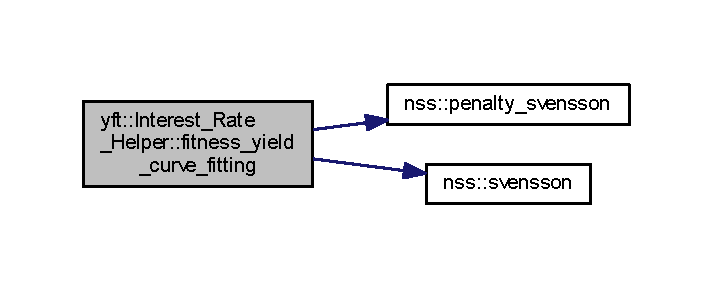
\includegraphics[width=342pt]{classyft_1_1_interest___rate___helper_ab8f50bcc6788356b008716a44dc134b8_cgraph}
\end{center}
\end{figure}
\mbox{\Hypertarget{classyft_1_1_interest___rate___helper_a2bf0217c985329f0f32c9df92b29456c}\label{classyft_1_1_interest___rate___helper_a2bf0217c985329f0f32c9df92b29456c}} 
\index{yft\+::\+Interest\+\_\+\+Rate\+\_\+\+Helper@{yft\+::\+Interest\+\_\+\+Rate\+\_\+\+Helper}!yieldcurve\+\_\+fitting@{yieldcurve\+\_\+fitting}}
\index{yieldcurve\+\_\+fitting@{yieldcurve\+\_\+fitting}!yft\+::\+Interest\+\_\+\+Rate\+\_\+\+Helper@{yft\+::\+Interest\+\_\+\+Rate\+\_\+\+Helper}}
\subsubsection{\texorpdfstring{yieldcurve\+\_\+fitting()}{yieldcurve\_fitting()}}
{\footnotesize\ttfamily template$<$typename T $>$ \\
template$<$typename S $>$ \\
\hyperlink{classyft_1_1_interest___rate___helper}{yft\+::\+Interest\+\_\+\+Rate\+\_\+\+Helper}$<$ T $>$\+::yieldcurve\+\_\+fitting (\begin{DoxyParamCaption}\item[{const S \&}]{solver }\end{DoxyParamCaption})\hspace{0.3cm}{\ttfamily [inline]}}



Yield Curve Fitting using interest rates and recorded periods. 


\begin{DoxyParams}{Parameters}
{\em solver} & The parameter structure of the solver that is going to be used for yield curve fitting \\
\hline
\end{DoxyParams}
\begin{DoxyReturn}{Returns}
void 
\end{DoxyReturn}


Definition at line 81 of file yield\+\_\+curve\+\_\+fitting.\+h.



References nss\+::constraints\+\_\+svensson(), ea\+::solve(), and nss\+::svensson().


\begin{DoxyCode}
82         \{
83             assert(solver.ndv == 6);
84             \textcolor{keyword}{auto} f = [&, use\_penalty\_method = solver.use\_penalty\_method](\textcolor{keyword}{const} \textcolor{keyword}{auto}& solution) \{ \textcolor{keywordflow}{return} 
      \hyperlink{classyft_1_1_interest___rate___helper_ab8f50bcc6788356b008716a44dc134b8}{fitness\_yield\_curve\_fitting}(solution, use\_penalty\_method); \};
85             \textcolor{keyword}{auto} c = [&, constraints\_type = solver.constraints\_type](\textcolor{keyword}{const} \textcolor{keyword}{auto}& solution) \{ \textcolor{keywordflow}{return} 
      \hyperlink{namespacenss_a39de3569a71e773f9da82c713eb7e6eb}{constraints\_svensson}(solution, constraints\_type); \};
86             std::cout << \textcolor{stringliteral}{"Yield Curve fitting."} << \textcolor{stringliteral}{"\(\backslash\)n"};
87             \textcolor{keyword}{auto} res = \hyperlink{namespaceea_a6450b5bf61e9fdca8b6c19267e14c560}{solve}(f, c, solver, \textcolor{stringliteral}{"YFT"});
88             T error = 0;
89             \textcolor{keywordflow}{for} (\textcolor{keyword}{const} \textcolor{keyword}{auto}& p : \hyperlink{classyft_1_1_interest___rate___helper_aaa22a1a41fd5eead9ea61136ebc8446c}{ir\_vec})
90             \{
91                 error = error + std::pow(\hyperlink{namespacenss_a71aad246261afa16f8bb1a4057570d4b}{svensson}(res, p.period) - p.rate, 2);
92                 \textcolor{comment}{//std::cout << "Estimated interest rates: " << svensson(res, p.period) << " Actual interest
       rates: " << p.rate << "\(\backslash\)n";}
93             \}
94             std::cout << \textcolor{stringliteral}{"Zero-rate Mean Squared Error: "} << error / ir\_vec.size() << \textcolor{stringliteral}{"\(\backslash\)n"};
95         \};
\end{DoxyCode}
Here is the call graph for this function\+:
\nopagebreak
\begin{figure}[H]
\begin{center}
\leavevmode
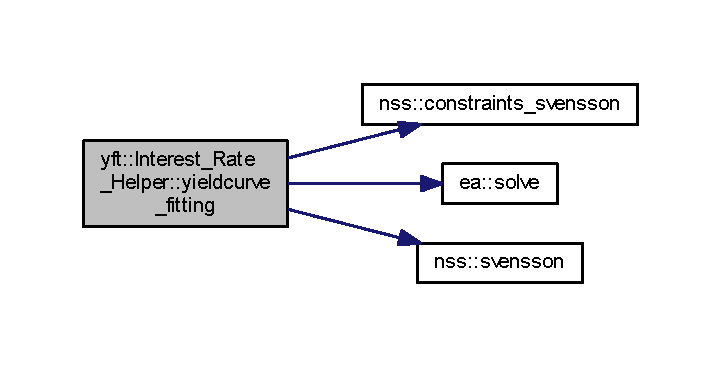
\includegraphics[width=346pt]{classyft_1_1_interest___rate___helper_a2bf0217c985329f0f32c9df92b29456c_cgraph}
\end{center}
\end{figure}


\subsection{Member Data Documentation}
\mbox{\Hypertarget{classyft_1_1_interest___rate___helper_aaa22a1a41fd5eead9ea61136ebc8446c}\label{classyft_1_1_interest___rate___helper_aaa22a1a41fd5eead9ea61136ebc8446c}} 
\index{yft\+::\+Interest\+\_\+\+Rate\+\_\+\+Helper@{yft\+::\+Interest\+\_\+\+Rate\+\_\+\+Helper}!ir\+\_\+vec@{ir\+\_\+vec}}
\index{ir\+\_\+vec@{ir\+\_\+vec}!yft\+::\+Interest\+\_\+\+Rate\+\_\+\+Helper@{yft\+::\+Interest\+\_\+\+Rate\+\_\+\+Helper}}
\subsubsection{\texorpdfstring{ir\+\_\+vec}{ir\_vec}}
{\footnotesize\ttfamily template$<$typename T $>$ \\
std\+::vector$<$\hyperlink{structyft_1_1_interest___rate}{Interest\+\_\+\+Rate}$<$T$>$ $>$ \hyperlink{classyft_1_1_interest___rate___helper}{yft\+::\+Interest\+\_\+\+Rate\+\_\+\+Helper}$<$ T $>$\+::ir\+\_\+vec\hspace{0.3cm}{\ttfamily [private]}}



Vector of interest rates. 



Definition at line 95 of file yield\+\_\+curve\+\_\+fitting.\+h.



The documentation for this class was generated from the following file\+:\begin{DoxyCompactItemize}
\item 
\hyperlink{yield__curve__fitting_8h}{yield\+\_\+curve\+\_\+fitting.\+h}\end{DoxyCompactItemize}

\hypertarget{structea_1_1_p_s_ol}{}\section{ea\+:\+:P\+S\+Ol$<$ T $>$ Struct Template Reference}
\label{structea_1_1_p_s_ol}\index{ea\+::\+P\+S\+Ol$<$ T $>$@{ea\+::\+P\+S\+Ol$<$ T $>$}}


Local Best Particle Swarm Optimisation Structure, used in the actual algorithm and for type deduction.  




{\ttfamily \#include $<$lbestpso.\+h$>$}



Inheritance diagram for ea\+:\+:P\+S\+Ol$<$ T $>$\+:
\nopagebreak
\begin{figure}[H]
\begin{center}
\leavevmode
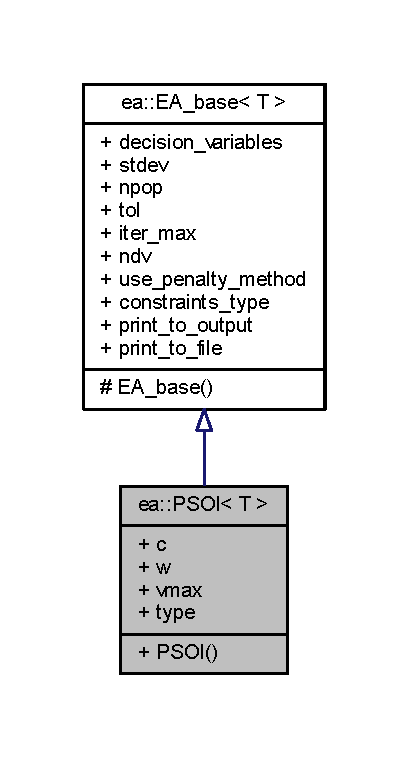
\includegraphics[width=196pt]{structea_1_1_p_s_ol__inherit__graph}
\end{center}
\end{figure}
\subsection*{Public Member Functions}
\begin{DoxyCompactItemize}
\item 
\hyperlink{structea_1_1_p_s_ol_ab0374356be7c06c8aae9092970f3525e}{P\+S\+Ol} (const T \&i\+\_\+c, const T \&i\+\_\+w, const std\+::vector$<$ T $>$ \&i\+\_\+vmax, const std\+::vector$<$ T $>$ \&i\+\_\+decision\+\_\+variables, const std\+::vector$<$ T $>$ \&i\+\_\+stdev, const size\+\_\+t \&i\+\_\+npop, const T \&i\+\_\+tol, const size\+\_\+t \&i\+\_\+iter\+\_\+max, const bool \&i\+\_\+use\+\_\+penalty\+\_\+method, const \hyperlink{namespaceutilities_ab1a1517bf6e62a1acfab5293ca8985c1}{Constraints\+\_\+type} \&i\+\_\+constraints\+\_\+type, const bool \&i\+\_\+print\+\_\+to\+\_\+output, const bool \&i\+\_\+print\+\_\+to\+\_\+file)
\begin{DoxyCompactList}\small\item\em Constructor. \end{DoxyCompactList}\end{DoxyCompactItemize}
\subsection*{Public Attributes}
\begin{DoxyCompactItemize}
\item 
const T \hyperlink{structea_1_1_p_s_ol_a7be4dc6b98fb6b991a69ad1c2275fffa}{c}
\begin{DoxyCompactList}\small\item\em Parameter c for velocity update. \end{DoxyCompactList}\item 
const T \hyperlink{structea_1_1_p_s_ol_a0c4742b6ff551a0c616fc64e093e6611}{w}
\begin{DoxyCompactList}\small\item\em Inertia Variant of P\+SO \+: Inertia. \end{DoxyCompactList}\item 
const std\+::vector$<$ T $>$ \hyperlink{structea_1_1_p_s_ol_a426318723c134f47004407c3f3ab79ce}{vmax}
\begin{DoxyCompactList}\small\item\em Velocity Clamping Variant of P\+SO \+: Maximum Velocity. \end{DoxyCompactList}\item 
const std\+::string \hyperlink{structea_1_1_p_s_ol_ad45c22065d096770d48b1c9e99dfd4fc}{type} = \char`\"{}Local Best Particle Swarm Optimisation\char`\"{}
\begin{DoxyCompactList}\small\item\em Type of the algorithm. \end{DoxyCompactList}\end{DoxyCompactItemize}
\subsection*{Additional Inherited Members}


\subsection{Detailed Description}
\subsubsection*{template$<$typename T$>$\newline
struct ea\+::\+P\+S\+Ol$<$ T $>$}

Local Best Particle Swarm Optimisation Structure, used in the actual algorithm and for type deduction. 

Definition at line 19 of file lbestpso.\+h.



\subsection{Constructor \& Destructor Documentation}
\mbox{\Hypertarget{structea_1_1_p_s_ol_ab0374356be7c06c8aae9092970f3525e}\label{structea_1_1_p_s_ol_ab0374356be7c06c8aae9092970f3525e}} 
\index{ea\+::\+P\+S\+Ol@{ea\+::\+P\+S\+Ol}!P\+S\+Ol@{P\+S\+Ol}}
\index{P\+S\+Ol@{P\+S\+Ol}!ea\+::\+P\+S\+Ol@{ea\+::\+P\+S\+Ol}}
\subsubsection{\texorpdfstring{P\+S\+Ol()}{PSOl()}}
{\footnotesize\ttfamily template$<$typename T$>$ \\
\hyperlink{structea_1_1_p_s_ol}{ea\+::\+P\+S\+Ol}$<$ T $>$\+::\hyperlink{structea_1_1_p_s_ol}{P\+S\+Ol} (\begin{DoxyParamCaption}\item[{const T \&}]{i\+\_\+c,  }\item[{const T \&}]{i\+\_\+w,  }\item[{const std\+::vector$<$ T $>$ \&}]{i\+\_\+vmax,  }\item[{const std\+::vector$<$ T $>$ \&}]{i\+\_\+decision\+\_\+variables,  }\item[{const std\+::vector$<$ T $>$ \&}]{i\+\_\+stdev,  }\item[{const size\+\_\+t \&}]{i\+\_\+npop,  }\item[{const T \&}]{i\+\_\+tol,  }\item[{const size\+\_\+t \&}]{i\+\_\+iter\+\_\+max,  }\item[{const bool \&}]{i\+\_\+use\+\_\+penalty\+\_\+method = {\ttfamily false},  }\item[{const \hyperlink{namespaceutilities_ab1a1517bf6e62a1acfab5293ca8985c1}{Constraints\+\_\+type} \&}]{i\+\_\+constraints\+\_\+type = {\ttfamily \hyperlink{namespaceea_a8e369877773b4db67b8512efdb4f8f89a334c4a4c42fdb79d7ebc3e73b517e6f8}{Constraints\+\_\+type\+::none}},  }\item[{const bool \&}]{i\+\_\+print\+\_\+to\+\_\+output = {\ttfamily true},  }\item[{const bool \&}]{i\+\_\+print\+\_\+to\+\_\+file = {\ttfamily true} }\end{DoxyParamCaption})\hspace{0.3cm}{\ttfamily [inline]}}



Constructor. 


\begin{DoxyParams}{Parameters}
{\em i\+\_\+c} & c parameter for velocity update \\
\hline
{\em i\+\_\+w} & Inertia parameter for velocity update \\
\hline
{\em i\+\_\+vmax} & Maximum velocity \\
\hline
{\em i\+\_\+decision\+\_\+variables} & The starting values of the decision variables \\
\hline
{\em i\+\_\+stdev} & The standard deviation \\
\hline
{\em i\+\_\+npop} & The population size \\
\hline
{\em i\+\_\+tol} & The tolerance \\
\hline
{\em i\+\_\+iter\+\_\+max} & The maximum number of iterations \\
\hline
{\em i\+\_\+use\+\_\+penalty\+\_\+method} & Whether to used penalties or not \\
\hline
{\em i\+\_\+constraints\+\_\+type} & What kind of constraints to use \\
\hline
{\em i\+\_\+print\+\_\+to\+\_\+output} & Whether to print to terminal or not \\
\hline
{\em i\+\_\+print\+\_\+to\+\_\+file} & Whether to print to a file or not \\
\hline
\end{DoxyParams}
\begin{DoxyReturn}{Returns}
A P\+S\+Ol$<$\+T$>$ object 
\end{DoxyReturn}


Definition at line 41 of file lbestpso.\+h.



References ea\+::\+P\+S\+Ol$<$ T $>$\+::c, ea\+::\+E\+A\+\_\+base$<$ T $>$\+::ndv, ea\+::\+P\+S\+Ol$<$ T $>$\+::vmax, and ea\+::\+P\+S\+Ol$<$ T $>$\+::w.


\begin{DoxyCode}
44                                                                         :
45             EA\_base<T>(i\_decision\_variables, i\_stdev, i\_npop, i\_tol, i\_iter\_max, i\_use\_penalty\_method, 
      i\_constraints\_type, i\_print\_to\_output, i\_print\_to\_file),
46             \hyperlink{structea_1_1_p_s_ol_a7be4dc6b98fb6b991a69ad1c2275fffa}{c}(i\_c),
47             \hyperlink{structea_1_1_p_s_ol_a0c4742b6ff551a0c616fc64e093e6611}{w}(i\_w),
48             \hyperlink{structea_1_1_p_s_ol_a426318723c134f47004407c3f3ab79ce}{vmax}(i\_vmax)
49         \{
50             assert(\hyperlink{structea_1_1_p_s_ol_a7be4dc6b98fb6b991a69ad1c2275fffa}{c} > 0);
51             assert(\hyperlink{structea_1_1_p_s_ol_a0c4742b6ff551a0c616fc64e093e6611}{w} > 0);
52             \textcolor{keywordflow}{for} (\textcolor{keyword}{const} \textcolor{keyword}{auto}& p : \hyperlink{structea_1_1_p_s_ol_a426318723c134f47004407c3f3ab79ce}{vmax}) \{ assert(p > 0); \};
53             assert(vmax.size() == this->\hyperlink{structea_1_1_e_a__base_a6996abed1c0b9642bdae67547fa6474c}{ndv});
54         \}
\end{DoxyCode}


\subsection{Member Data Documentation}
\mbox{\Hypertarget{structea_1_1_p_s_ol_a7be4dc6b98fb6b991a69ad1c2275fffa}\label{structea_1_1_p_s_ol_a7be4dc6b98fb6b991a69ad1c2275fffa}} 
\index{ea\+::\+P\+S\+Ol@{ea\+::\+P\+S\+Ol}!c@{c}}
\index{c@{c}!ea\+::\+P\+S\+Ol@{ea\+::\+P\+S\+Ol}}
\subsubsection{\texorpdfstring{c}{c}}
{\footnotesize\ttfamily template$<$typename T$>$ \\
const T \hyperlink{structea_1_1_p_s_ol}{ea\+::\+P\+S\+Ol}$<$ T $>$\+::c}



Parameter c for velocity update. 



Definition at line 56 of file lbestpso.\+h.



Referenced by ea\+::\+Solver$<$ P\+S\+Ol, T, F, C $>$\+::display\+\_\+parameters(), ea\+::\+Solver$<$ P\+S\+Ol, T, F, C $>$\+::position\+\_\+update(), and ea\+::\+P\+S\+Ol$<$ T $>$\+::\+P\+S\+Ol().

\mbox{\Hypertarget{structea_1_1_p_s_ol_ad45c22065d096770d48b1c9e99dfd4fc}\label{structea_1_1_p_s_ol_ad45c22065d096770d48b1c9e99dfd4fc}} 
\index{ea\+::\+P\+S\+Ol@{ea\+::\+P\+S\+Ol}!type@{type}}
\index{type@{type}!ea\+::\+P\+S\+Ol@{ea\+::\+P\+S\+Ol}}
\subsubsection{\texorpdfstring{type}{type}}
{\footnotesize\ttfamily template$<$typename T$>$ \\
const std\+::string \hyperlink{structea_1_1_p_s_ol}{ea\+::\+P\+S\+Ol}$<$ T $>$\+::type = \char`\"{}Local Best Particle Swarm Optimisation\char`\"{}}



Type of the algorithm. 



Definition at line 62 of file lbestpso.\+h.

\mbox{\Hypertarget{structea_1_1_p_s_ol_a426318723c134f47004407c3f3ab79ce}\label{structea_1_1_p_s_ol_a426318723c134f47004407c3f3ab79ce}} 
\index{ea\+::\+P\+S\+Ol@{ea\+::\+P\+S\+Ol}!vmax@{vmax}}
\index{vmax@{vmax}!ea\+::\+P\+S\+Ol@{ea\+::\+P\+S\+Ol}}
\subsubsection{\texorpdfstring{vmax}{vmax}}
{\footnotesize\ttfamily template$<$typename T$>$ \\
const std\+::vector$<$T$>$ \hyperlink{structea_1_1_p_s_ol}{ea\+::\+P\+S\+Ol}$<$ T $>$\+::vmax}



Velocity Clamping Variant of P\+SO \+: Maximum Velocity. 



Definition at line 60 of file lbestpso.\+h.



Referenced by ea\+::\+Solver$<$ P\+S\+Ol, T, F, C $>$\+::display\+\_\+parameters(), ea\+::\+Solver$<$ P\+S\+Ol, T, F, C $>$\+::position\+\_\+update(), and ea\+::\+P\+S\+Ol$<$ T $>$\+::\+P\+S\+Ol().

\mbox{\Hypertarget{structea_1_1_p_s_ol_a0c4742b6ff551a0c616fc64e093e6611}\label{structea_1_1_p_s_ol_a0c4742b6ff551a0c616fc64e093e6611}} 
\index{ea\+::\+P\+S\+Ol@{ea\+::\+P\+S\+Ol}!w@{w}}
\index{w@{w}!ea\+::\+P\+S\+Ol@{ea\+::\+P\+S\+Ol}}
\subsubsection{\texorpdfstring{w}{w}}
{\footnotesize\ttfamily template$<$typename T$>$ \\
const T \hyperlink{structea_1_1_p_s_ol}{ea\+::\+P\+S\+Ol}$<$ T $>$\+::w}



Inertia Variant of P\+SO \+: Inertia. 



Definition at line 58 of file lbestpso.\+h.



Referenced by ea\+::\+Solver$<$ P\+S\+Ol, T, F, C $>$\+::display\+\_\+parameters(), ea\+::\+Solver$<$ P\+S\+Ol, T, F, C $>$\+::position\+\_\+update(), ea\+::\+P\+S\+Ol$<$ T $>$\+::\+P\+S\+Ol(), and ea\+::\+Solver$<$ P\+S\+Ol, T, F, C $>$\+::run\+\_\+algo().



The documentation for this struct was generated from the following file\+:\begin{DoxyCompactItemize}
\item 
\hyperlink{lbestpso_8h}{lbestpso.\+h}\end{DoxyCompactItemize}

\hypertarget{structea_1_1_p_s_os}{}\section{ea\+:\+:P\+S\+Os$<$ T $>$ Struct Template Reference}
\label{structea_1_1_p_s_os}\index{ea\+::\+P\+S\+Os$<$ T $>$@{ea\+::\+P\+S\+Os$<$ T $>$}}


Particle Swarm Optimisation Structure, used in the actual algorithm and for type deduction.  




{\ttfamily \#include $<$pso\+\_\+sub\+\_\+swarm.\+h$>$}



Inheritance diagram for ea\+:\+:P\+S\+Os$<$ T $>$\+:
\nopagebreak
\begin{figure}[H]
\begin{center}
\leavevmode
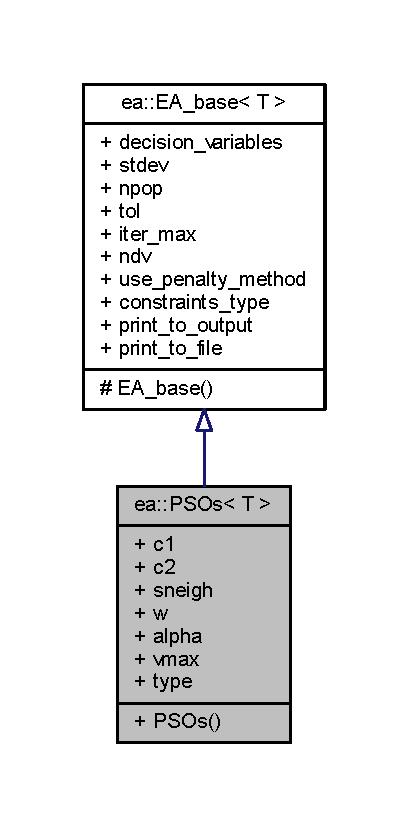
\includegraphics[width=196pt]{structea_1_1_p_s_os__inherit__graph}
\end{center}
\end{figure}
\subsection*{Public Member Functions}
\begin{DoxyCompactItemize}
\item 
\hyperlink{structea_1_1_p_s_os_ae9c6e48cd827aadb4463101211baaa16}{P\+S\+Os} (const T \&i\+\_\+c1, const T \&i\+\_\+c2, const size\+\_\+t \&i\+\_\+sneigh, const T \&i\+\_\+w, const T \&i\+\_\+alpha, const std\+::vector$<$ T $>$ \&i\+\_\+vmax, const std\+::vector$<$ T $>$ \&i\+\_\+decision\+\_\+variables, const std\+::vector$<$ T $>$ \&i\+\_\+stdev, const size\+\_\+t \&i\+\_\+npop, const T \&i\+\_\+tol, const size\+\_\+t \&i\+\_\+iter\+\_\+max, const bool \&i\+\_\+use\+\_\+penalty\+\_\+method, const \hyperlink{namespaceutilities_ab1a1517bf6e62a1acfab5293ca8985c1}{Constraints\+\_\+type} \&i\+\_\+constraints\+\_\+type, const bool \&i\+\_\+print\+\_\+to\+\_\+output, const bool \&i\+\_\+print\+\_\+to\+\_\+file)
\begin{DoxyCompactList}\small\item\em Constructor. \end{DoxyCompactList}\end{DoxyCompactItemize}
\subsection*{Public Attributes}
\begin{DoxyCompactItemize}
\item 
const T \hyperlink{structea_1_1_p_s_os_ad714859d3155b4492fb01eb1664e7c65}{c1}
\begin{DoxyCompactList}\small\item\em Parameter c1 for velocity update. \end{DoxyCompactList}\item 
const T \hyperlink{structea_1_1_p_s_os_a905b431f08e1617a0e30bdac1093927b}{c2}
\begin{DoxyCompactList}\small\item\em Parameter c2 for velocity update. \end{DoxyCompactList}\item 
const size\+\_\+t \hyperlink{structea_1_1_p_s_os_a60d85bb8fdc3913239c5769906c3f917}{sneigh}
\begin{DoxyCompactList}\small\item\em Neighbourhood size. \end{DoxyCompactList}\item 
const T \hyperlink{structea_1_1_p_s_os_a31794d89fb98ef9f4e887458c0982982}{w}
\begin{DoxyCompactList}\small\item\em Inertia Variant of P\+SO \+: Inertia. \end{DoxyCompactList}\item 
const T \hyperlink{structea_1_1_p_s_os_ae12721e5571bed1300a16dac83ab27cc}{alpha}
\begin{DoxyCompactList}\small\item\em Alpha Parameter for maximum velocity. \end{DoxyCompactList}\item 
const std\+::vector$<$ T $>$ \hyperlink{structea_1_1_p_s_os_a58dfadd4951b668607176b290a18c1fa}{vmax}
\begin{DoxyCompactList}\small\item\em Velocity Clamping Variant of P\+SO \+: Maximum Velocity. \end{DoxyCompactList}\item 
const std\+::string \hyperlink{structea_1_1_p_s_os_a70f9529943125d7f2811961e1d25b30b}{type} = \char`\"{}Sub-\/swarm Particle Swarm Optimisation\char`\"{}
\begin{DoxyCompactList}\small\item\em Type of the algorithm. \end{DoxyCompactList}\end{DoxyCompactItemize}
\subsection*{Additional Inherited Members}


\subsection{Detailed Description}
\subsubsection*{template$<$typename T$>$\newline
struct ea\+::\+P\+S\+Os$<$ T $>$}

Particle Swarm Optimisation Structure, used in the actual algorithm and for type deduction. 

Definition at line 17 of file pso\+\_\+sub\+\_\+swarm.\+h.



\subsection{Constructor \& Destructor Documentation}
\mbox{\Hypertarget{structea_1_1_p_s_os_ae9c6e48cd827aadb4463101211baaa16}\label{structea_1_1_p_s_os_ae9c6e48cd827aadb4463101211baaa16}} 
\index{ea\+::\+P\+S\+Os@{ea\+::\+P\+S\+Os}!P\+S\+Os@{P\+S\+Os}}
\index{P\+S\+Os@{P\+S\+Os}!ea\+::\+P\+S\+Os@{ea\+::\+P\+S\+Os}}
\subsubsection{\texorpdfstring{P\+S\+Os()}{PSOs()}}
{\footnotesize\ttfamily template$<$typename T$>$ \\
\hyperlink{structea_1_1_p_s_os}{ea\+::\+P\+S\+Os}$<$ T $>$\+::\hyperlink{structea_1_1_p_s_os}{P\+S\+Os} (\begin{DoxyParamCaption}\item[{const T \&}]{i\+\_\+c1,  }\item[{const T \&}]{i\+\_\+c2,  }\item[{const size\+\_\+t \&}]{i\+\_\+sneigh,  }\item[{const T \&}]{i\+\_\+w,  }\item[{const T \&}]{i\+\_\+alpha,  }\item[{const std\+::vector$<$ T $>$ \&}]{i\+\_\+vmax,  }\item[{const std\+::vector$<$ T $>$ \&}]{i\+\_\+decision\+\_\+variables,  }\item[{const std\+::vector$<$ T $>$ \&}]{i\+\_\+stdev,  }\item[{const size\+\_\+t \&}]{i\+\_\+npop,  }\item[{const T \&}]{i\+\_\+tol,  }\item[{const size\+\_\+t \&}]{i\+\_\+iter\+\_\+max,  }\item[{const bool \&}]{i\+\_\+use\+\_\+penalty\+\_\+method = {\ttfamily false},  }\item[{const \hyperlink{namespaceutilities_ab1a1517bf6e62a1acfab5293ca8985c1}{Constraints\+\_\+type} \&}]{i\+\_\+constraints\+\_\+type = {\ttfamily \hyperlink{namespaceea_a8e369877773b4db67b8512efdb4f8f89a334c4a4c42fdb79d7ebc3e73b517e6f8}{Constraints\+\_\+type\+::none}},  }\item[{const bool \&}]{i\+\_\+print\+\_\+to\+\_\+output = {\ttfamily true},  }\item[{const bool \&}]{i\+\_\+print\+\_\+to\+\_\+file = {\ttfamily true} }\end{DoxyParamCaption})\hspace{0.3cm}{\ttfamily [inline]}}



Constructor. 


\begin{DoxyParams}{Parameters}
{\em i\+\_\+c1} & c1 parameter for velocity update \\
\hline
{\em i\+\_\+c2} & c2 parameter for velocity update \\
\hline
{\em i\+\_\+sneigh} & Number of neighbourhoods \\
\hline
{\em i\+\_\+w} & Inertia parameter for velocity update \\
\hline
{\em i\+\_\+alpha} & alpha parameter for maximum velocity decrease \\
\hline
{\em i\+\_\+vmax} & Maximum velocity \\
\hline
{\em i\+\_\+decision\+\_\+variables} & The starting values of the decision variables \\
\hline
{\em i\+\_\+stdev} & The standard deviation \\
\hline
{\em i\+\_\+npop} & The population size \\
\hline
{\em i\+\_\+tol} & The tolerance \\
\hline
{\em i\+\_\+iter\+\_\+max} & The maximum number of iterations \\
\hline
{\em i\+\_\+use\+\_\+penalty\+\_\+method} & Whether to used penalties or not \\
\hline
{\em i\+\_\+constraints\+\_\+type} & What kind of constraints to use \\
\hline
{\em i\+\_\+print\+\_\+to\+\_\+output} & Whether to print to terminal or not \\
\hline
{\em i\+\_\+print\+\_\+to\+\_\+file} & Whether to print to a file or not \\
\hline
\end{DoxyParams}
\begin{DoxyReturn}{Returns}
A P\+S\+O$<$\+T$>$ object 
\end{DoxyReturn}


Definition at line 42 of file pso\+\_\+sub\+\_\+swarm.\+h.



References ea\+::\+P\+S\+Os$<$ T $>$\+::alpha, ea\+::\+P\+S\+Os$<$ T $>$\+::c1, ea\+::\+P\+S\+Os$<$ T $>$\+::c2, ea\+::\+E\+A\+\_\+base$<$ T $>$\+::ndv, ea\+::\+P\+S\+Os$<$ T $>$\+::sneigh, ea\+::\+P\+S\+Os$<$ T $>$\+::vmax, and ea\+::\+P\+S\+Os$<$ T $>$\+::w.


\begin{DoxyCode}
45                                                                         :
46             EA\_base<T>(i\_decision\_variables, i\_stdev, i\_npop, i\_tol, i\_iter\_max, i\_use\_penalty\_method, 
      i\_constraints\_type, i\_print\_to\_output, i\_print\_to\_file),
47             \hyperlink{structea_1_1_p_s_os_ad714859d3155b4492fb01eb1664e7c65}{c1}( i\_c1 ),
48             \hyperlink{structea_1_1_p_s_os_a905b431f08e1617a0e30bdac1093927b}{c2}( i\_c2 ), 
49             \hyperlink{structea_1_1_p_s_os_a60d85bb8fdc3913239c5769906c3f917}{sneigh}( i\_sneigh ), 
50             \hyperlink{structea_1_1_p_s_os_a31794d89fb98ef9f4e887458c0982982}{w}( i\_w ), 
51             \hyperlink{structea_1_1_p_s_os_ae12721e5571bed1300a16dac83ab27cc}{alpha}( i\_alpha ), 
52             \hyperlink{structea_1_1_p_s_os_a58dfadd4951b668607176b290a18c1fa}{vmax}( i\_vmax )
53         \{
54             assert(\hyperlink{structea_1_1_p_s_os_ad714859d3155b4492fb01eb1664e7c65}{c1} > 0);
55             assert(\hyperlink{structea_1_1_p_s_os_a905b431f08e1617a0e30bdac1093927b}{c2} > 0);
56             assert(\hyperlink{structea_1_1_p_s_os_a60d85bb8fdc3913239c5769906c3f917}{sneigh} > 0);
57             assert(\hyperlink{structea_1_1_p_s_os_a60d85bb8fdc3913239c5769906c3f917}{sneigh} < i\_npop);
58             assert(\hyperlink{structea_1_1_p_s_os_a31794d89fb98ef9f4e887458c0982982}{w} > 0);
59             assert(\hyperlink{structea_1_1_p_s_os_ae12721e5571bed1300a16dac83ab27cc}{alpha} > 0);
60             \textcolor{keywordflow}{for} (\textcolor{keyword}{const} \textcolor{keyword}{auto}& p : \hyperlink{structea_1_1_p_s_os_a58dfadd4951b668607176b290a18c1fa}{vmax}) \{ assert(p > 0); \};
61             assert(vmax.size() == this->\hyperlink{structea_1_1_e_a__base_a6996abed1c0b9642bdae67547fa6474c}{ndv});
62         \}
\end{DoxyCode}


\subsection{Member Data Documentation}
\mbox{\Hypertarget{structea_1_1_p_s_os_ae12721e5571bed1300a16dac83ab27cc}\label{structea_1_1_p_s_os_ae12721e5571bed1300a16dac83ab27cc}} 
\index{ea\+::\+P\+S\+Os@{ea\+::\+P\+S\+Os}!alpha@{alpha}}
\index{alpha@{alpha}!ea\+::\+P\+S\+Os@{ea\+::\+P\+S\+Os}}
\subsubsection{\texorpdfstring{alpha}{alpha}}
{\footnotesize\ttfamily template$<$typename T$>$ \\
const T \hyperlink{structea_1_1_p_s_os}{ea\+::\+P\+S\+Os}$<$ T $>$\+::alpha}



Alpha Parameter for maximum velocity. 



Definition at line 72 of file pso\+\_\+sub\+\_\+swarm.\+h.



Referenced by ea\+::\+Solver$<$ P\+S\+Os, T, F, C $>$\+::display\+\_\+parameters(), and ea\+::\+P\+S\+Os$<$ T $>$\+::\+P\+S\+Os().

\mbox{\Hypertarget{structea_1_1_p_s_os_ad714859d3155b4492fb01eb1664e7c65}\label{structea_1_1_p_s_os_ad714859d3155b4492fb01eb1664e7c65}} 
\index{ea\+::\+P\+S\+Os@{ea\+::\+P\+S\+Os}!c1@{c1}}
\index{c1@{c1}!ea\+::\+P\+S\+Os@{ea\+::\+P\+S\+Os}}
\subsubsection{\texorpdfstring{c1}{c1}}
{\footnotesize\ttfamily template$<$typename T$>$ \\
const T \hyperlink{structea_1_1_p_s_os}{ea\+::\+P\+S\+Os}$<$ T $>$\+::c1}



Parameter c1 for velocity update. 



Definition at line 64 of file pso\+\_\+sub\+\_\+swarm.\+h.



Referenced by ea\+::\+Solver$<$ P\+S\+Os, T, F, C $>$\+::display\+\_\+parameters(), and ea\+::\+P\+S\+Os$<$ T $>$\+::\+P\+S\+Os().

\mbox{\Hypertarget{structea_1_1_p_s_os_a905b431f08e1617a0e30bdac1093927b}\label{structea_1_1_p_s_os_a905b431f08e1617a0e30bdac1093927b}} 
\index{ea\+::\+P\+S\+Os@{ea\+::\+P\+S\+Os}!c2@{c2}}
\index{c2@{c2}!ea\+::\+P\+S\+Os@{ea\+::\+P\+S\+Os}}
\subsubsection{\texorpdfstring{c2}{c2}}
{\footnotesize\ttfamily template$<$typename T$>$ \\
const T \hyperlink{structea_1_1_p_s_os}{ea\+::\+P\+S\+Os}$<$ T $>$\+::c2}



Parameter c2 for velocity update. 



Definition at line 66 of file pso\+\_\+sub\+\_\+swarm.\+h.



Referenced by ea\+::\+Solver$<$ P\+S\+Os, T, F, C $>$\+::display\+\_\+parameters(), and ea\+::\+P\+S\+Os$<$ T $>$\+::\+P\+S\+Os().

\mbox{\Hypertarget{structea_1_1_p_s_os_a60d85bb8fdc3913239c5769906c3f917}\label{structea_1_1_p_s_os_a60d85bb8fdc3913239c5769906c3f917}} 
\index{ea\+::\+P\+S\+Os@{ea\+::\+P\+S\+Os}!sneigh@{sneigh}}
\index{sneigh@{sneigh}!ea\+::\+P\+S\+Os@{ea\+::\+P\+S\+Os}}
\subsubsection{\texorpdfstring{sneigh}{sneigh}}
{\footnotesize\ttfamily template$<$typename T$>$ \\
const size\+\_\+t \hyperlink{structea_1_1_p_s_os}{ea\+::\+P\+S\+Os}$<$ T $>$\+::sneigh}



Neighbourhood size. 



Definition at line 68 of file pso\+\_\+sub\+\_\+swarm.\+h.



Referenced by ea\+::\+Solver$<$ P\+S\+Os, T, F, C $>$\+::display\+\_\+parameters(), and ea\+::\+P\+S\+Os$<$ T $>$\+::\+P\+S\+Os().

\mbox{\Hypertarget{structea_1_1_p_s_os_a70f9529943125d7f2811961e1d25b30b}\label{structea_1_1_p_s_os_a70f9529943125d7f2811961e1d25b30b}} 
\index{ea\+::\+P\+S\+Os@{ea\+::\+P\+S\+Os}!type@{type}}
\index{type@{type}!ea\+::\+P\+S\+Os@{ea\+::\+P\+S\+Os}}
\subsubsection{\texorpdfstring{type}{type}}
{\footnotesize\ttfamily template$<$typename T$>$ \\
const std\+::string \hyperlink{structea_1_1_p_s_os}{ea\+::\+P\+S\+Os}$<$ T $>$\+::type = \char`\"{}Sub-\/swarm Particle Swarm Optimisation\char`\"{}}



Type of the algorithm. 



Definition at line 76 of file pso\+\_\+sub\+\_\+swarm.\+h.

\mbox{\Hypertarget{structea_1_1_p_s_os_a58dfadd4951b668607176b290a18c1fa}\label{structea_1_1_p_s_os_a58dfadd4951b668607176b290a18c1fa}} 
\index{ea\+::\+P\+S\+Os@{ea\+::\+P\+S\+Os}!vmax@{vmax}}
\index{vmax@{vmax}!ea\+::\+P\+S\+Os@{ea\+::\+P\+S\+Os}}
\subsubsection{\texorpdfstring{vmax}{vmax}}
{\footnotesize\ttfamily template$<$typename T$>$ \\
const std\+::vector$<$T$>$ \hyperlink{structea_1_1_p_s_os}{ea\+::\+P\+S\+Os}$<$ T $>$\+::vmax}



Velocity Clamping Variant of P\+SO \+: Maximum Velocity. 



Definition at line 74 of file pso\+\_\+sub\+\_\+swarm.\+h.



Referenced by ea\+::\+Solver$<$ P\+S\+Os, T, F, C $>$\+::display\+\_\+parameters(), ea\+::\+Solver$<$ P\+S\+Os, T, F, C $>$\+::position\+\_\+update(), and ea\+::\+P\+S\+Os$<$ T $>$\+::\+P\+S\+Os().

\mbox{\Hypertarget{structea_1_1_p_s_os_a31794d89fb98ef9f4e887458c0982982}\label{structea_1_1_p_s_os_a31794d89fb98ef9f4e887458c0982982}} 
\index{ea\+::\+P\+S\+Os@{ea\+::\+P\+S\+Os}!w@{w}}
\index{w@{w}!ea\+::\+P\+S\+Os@{ea\+::\+P\+S\+Os}}
\subsubsection{\texorpdfstring{w}{w}}
{\footnotesize\ttfamily template$<$typename T$>$ \\
const T \hyperlink{structea_1_1_p_s_os}{ea\+::\+P\+S\+Os}$<$ T $>$\+::w}



Inertia Variant of P\+SO \+: Inertia. 



Definition at line 70 of file pso\+\_\+sub\+\_\+swarm.\+h.



Referenced by ea\+::\+Solver$<$ P\+S\+Os, T, F, C $>$\+::display\+\_\+parameters(), ea\+::\+P\+S\+Os$<$ T $>$\+::\+P\+S\+Os(), and ea\+::\+Solver$<$ P\+S\+Os, T, F, C $>$\+::run\+\_\+algo().



The documentation for this struct was generated from the following file\+:\begin{DoxyCompactItemize}
\item 
\hyperlink{pso__sub__swarm_8h}{pso\+\_\+sub\+\_\+swarm.\+h}\end{DoxyCompactItemize}

\hypertarget{classea_1_1_solver}{}\section{ea\+:\+:Solver$<$ S, T, F, C $>$ Class Template Reference}
\label{classea_1_1_solver}\index{ea\+::\+Solver$<$ S, T, F, C $>$@{ea\+::\+Solver$<$ S, T, F, C $>$}}


Template Class for Solvers.  




{\ttfamily \#include $<$ealgorithm\+\_\+base.\+h$>$}



\subsection{Detailed Description}
\subsubsection*{template$<$template$<$ typename $>$ class S, typename T, typename F, typename C$>$\newline
class ea\+::\+Solver$<$ S, T, F, C $>$}

Template Class for Solvers. 

Definition at line 93 of file ealgorithm\+\_\+base.\+h.



The documentation for this class was generated from the following file\+:\begin{DoxyCompactItemize}
\item 
\hyperlink{ealgorithm__base_8h}{ealgorithm\+\_\+base.\+h}\end{DoxyCompactItemize}

\hypertarget{classea_1_1_solver_3_01_d_e_00_01_t_00_01_f_00_01_c_01_4}{}\section{ea\+:\+:Solver$<$ DE, T, F, C $>$ Class Template Reference}
\label{classea_1_1_solver_3_01_d_e_00_01_t_00_01_f_00_01_c_01_4}\index{ea\+::\+Solver$<$ D\+E, T, F, C $>$@{ea\+::\+Solver$<$ D\+E, T, F, C $>$}}


Differential Evolution Algorithm (\hyperlink{structea_1_1_d_e}{DE}) Class.  




{\ttfamily \#include $<$differentialevo.\+h$>$}



Inheritance diagram for ea\+:\+:Solver$<$ DE, T, F, C $>$\+:
\nopagebreak
\begin{figure}[H]
\begin{center}
\leavevmode
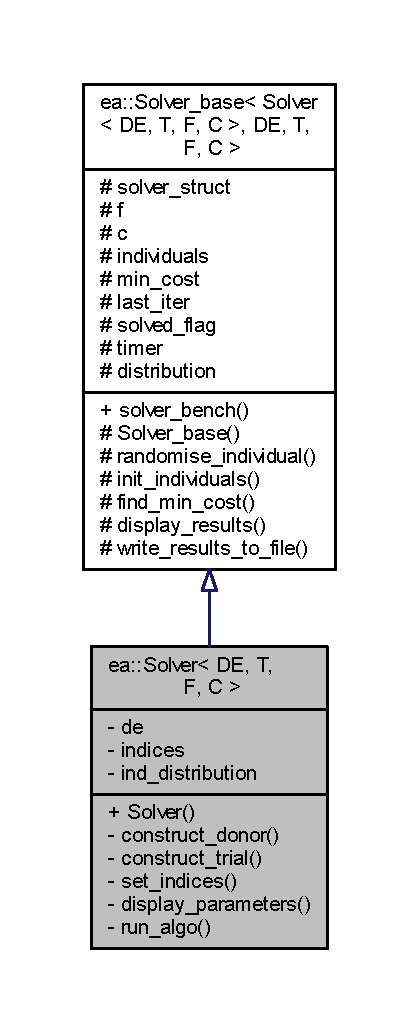
\includegraphics[width=201pt]{classea_1_1_solver_3_01_d_e_00_01_t_00_01_f_00_01_c_01_4__inherit__graph}
\end{center}
\end{figure}
\subsection*{Public Member Functions}
\begin{DoxyCompactItemize}
\item 
\hyperlink{classea_1_1_solver_3_01_d_e_00_01_t_00_01_f_00_01_c_01_4_ae960a525f47309ff0d90f8ac404e3599}{Solver} (const \hyperlink{structea_1_1_d_e}{DE}$<$ T $>$ \&i\+\_\+de, const F \&\hyperlink{classea_1_1_solver__base_ae0a893780c93dfe17c1d17301de6494f}{f}, const C \&\hyperlink{classea_1_1_solver__base_a6914e89d30e7484f2b4af1783f0de8c3}{c})
\begin{DoxyCompactList}\small\item\em Constructor. \end{DoxyCompactList}\end{DoxyCompactItemize}
\subsection*{Private Member Functions}
\begin{DoxyCompactItemize}
\item 
std\+::vector$<$ T $>$ \hyperlink{classea_1_1_solver_3_01_d_e_00_01_t_00_01_f_00_01_c_01_4_a69dabdddba116ddb5685355119bd77e0}{construct\+\_\+donor} ()
\begin{DoxyCompactList}\small\item\em Method that constructs the donor vector. \end{DoxyCompactList}\item 
std\+::vector$<$ T $>$ \hyperlink{classea_1_1_solver_3_01_d_e_00_01_t_00_01_f_00_01_c_01_4_a043f8134c53f09519283b8320d7a2ade}{construct\+\_\+trial} (const std\+::vector$<$ T $>$ \&target, const std\+::vector$<$ T $>$ \&donor)
\begin{DoxyCompactList}\small\item\em Method that constructs the trial vector. \end{DoxyCompactList}\item 
std\+::vector$<$ size\+\_\+t $>$ \hyperlink{classea_1_1_solver_3_01_d_e_00_01_t_00_01_f_00_01_c_01_4_a86a25b0977865969248efd4e79e4982f}{set\+\_\+indices} ()
\begin{DoxyCompactList}\small\item\em Generate the indices. \end{DoxyCompactList}\item 
std\+::stringstream \hyperlink{classea_1_1_solver_3_01_d_e_00_01_t_00_01_f_00_01_c_01_4_a122c904c555a0be3b27160d6f883fd1b}{display\+\_\+parameters} ()
\begin{DoxyCompactList}\small\item\em Display the parameters of \hyperlink{structea_1_1_d_e}{DE}. \end{DoxyCompactList}\item 
void \hyperlink{classea_1_1_solver_3_01_d_e_00_01_t_00_01_f_00_01_c_01_4_a6e560e4d8fb8f578ebe0fd7beb802632}{run\+\_\+algo} ()
\begin{DoxyCompactList}\small\item\em Runs the algorithm until stopping criteria return void. \end{DoxyCompactList}\end{DoxyCompactItemize}
\subsection*{Private Attributes}
\begin{DoxyCompactItemize}
\item 
const \hyperlink{structea_1_1_d_e}{DE}$<$ T $>$ \& \hyperlink{classea_1_1_solver_3_01_d_e_00_01_t_00_01_f_00_01_c_01_4_a789b8665ce321248e3999907c37d0963}{de}
\begin{DoxyCompactList}\small\item\em Differential Evolution structure used internally (reference to solver\+\_\+struct) \end{DoxyCompactList}\item 
const std\+::vector$<$ size\+\_\+t $>$ \hyperlink{classea_1_1_solver_3_01_d_e_00_01_t_00_01_f_00_01_c_01_4_a8428ecceaab1c7e26715ed2f72654693}{indices}
\begin{DoxyCompactList}\small\item\em Indices of population. \end{DoxyCompactList}\item 
std\+::uniform\+\_\+int\+\_\+distribution$<$ size\+\_\+t $>$ \hyperlink{classea_1_1_solver_3_01_d_e_00_01_t_00_01_f_00_01_c_01_4_a2f762378d566944899b2a07a5c74fc7f}{ind\+\_\+distribution}
\begin{DoxyCompactList}\small\item\em Uniform size\+\_\+t distribution of the indices. \end{DoxyCompactList}\end{DoxyCompactItemize}
\subsection*{Friends}
\begin{DoxyCompactItemize}
\item 
class \hyperlink{classea_1_1_solver_3_01_d_e_00_01_t_00_01_f_00_01_c_01_4_af331e622818a725800b24cd03d46f3f1}{Solver\+\_\+base$<$ Solver$<$ D\+E, T, F, C $>$, D\+E, T, F, C $>$}
\end{DoxyCompactItemize}
\subsection*{Additional Inherited Members}


\subsection{Detailed Description}
\subsubsection*{template$<$typename T, typename F, typename C$>$\newline
class ea\+::\+Solver$<$ D\+E, T, F, C $>$}

Differential Evolution Algorithm (\hyperlink{structea_1_1_d_e}{DE}) Class. 

Definition at line 60 of file differentialevo.\+h.



\subsection{Constructor \& Destructor Documentation}
\mbox{\Hypertarget{classea_1_1_solver_3_01_d_e_00_01_t_00_01_f_00_01_c_01_4_ae960a525f47309ff0d90f8ac404e3599}\label{classea_1_1_solver_3_01_d_e_00_01_t_00_01_f_00_01_c_01_4_ae960a525f47309ff0d90f8ac404e3599}} 
\index{ea\+::\+Solver$<$ D\+E, T, F, C $>$@{ea\+::\+Solver$<$ D\+E, T, F, C $>$}!Solver@{Solver}}
\index{Solver@{Solver}!ea\+::\+Solver$<$ D\+E, T, F, C $>$@{ea\+::\+Solver$<$ D\+E, T, F, C $>$}}
\subsubsection{\texorpdfstring{Solver()}{Solver()}}
{\footnotesize\ttfamily template$<$typename T , typename F , typename C $>$ \\
\hyperlink{classea_1_1_solver}{ea\+::\+Solver}$<$ \hyperlink{structea_1_1_d_e}{DE}, T, F, C $>$\+::\hyperlink{classea_1_1_solver}{Solver} (\begin{DoxyParamCaption}\item[{const \hyperlink{structea_1_1_d_e}{DE}$<$ T $>$ \&}]{i\+\_\+de,  }\item[{const F \&}]{f,  }\item[{const C \&}]{c }\end{DoxyParamCaption})\hspace{0.3cm}{\ttfamily [inline]}}



Constructor. 


\begin{DoxyParams}{Parameters}
{\em i\+\_\+de} & The differential evolution parameter structure that is used to construct the solver \\
\hline
{\em f} & A reference to the objective function \\
\hline
{\em c} & A reference to the constraints function \\
\hline
\end{DoxyParams}
\begin{DoxyReturn}{Returns}
A \hyperlink{classea_1_1_solver_3_01_d_e_00_01_t_00_01_f_00_01_c_01_4}{Solver$<$\+D\+E, T, F, C$>$} object 
\end{DoxyReturn}


Definition at line 71 of file differentialevo.\+h.


\begin{DoxyCode}
71                                                           :
72                 Solver\_base<Solver<DE, T, F, C>, DE, T, F, C>( i\_de, \hyperlink{classea_1_1_solver__base_ae0a893780c93dfe17c1d17301de6494f}{f}, \hyperlink{classea_1_1_solver__base_a6914e89d30e7484f2b4af1783f0de8c3}{c} ),
73                 \hyperlink{classea_1_1_solver_3_01_d_e_00_01_t_00_01_f_00_01_c_01_4_a789b8665ce321248e3999907c37d0963}{de}( this->\hyperlink{classea_1_1_solver__base_a5e1d821809f2d26c6f882942ad728127}{solver\_struct} ),
74                 \hyperlink{classea_1_1_solver_3_01_d_e_00_01_t_00_01_f_00_01_c_01_4_a8428ecceaab1c7e26715ed2f72654693}{indices}( \hyperlink{classea_1_1_solver_3_01_d_e_00_01_t_00_01_f_00_01_c_01_4_a86a25b0977865969248efd4e79e4982f}{set\_indices}() ),
75                 \hyperlink{classea_1_1_solver_3_01_d_e_00_01_t_00_01_f_00_01_c_01_4_a2f762378d566944899b2a07a5c74fc7f}{ind\_distribution}( std::uniform\_int\_distribution<size\_t>(0,
      \hyperlink{classea_1_1_solver_3_01_d_e_00_01_t_00_01_f_00_01_c_01_4_a789b8665ce321248e3999907c37d0963}{de}.npop - 1) )
76         \{
77         \};
\end{DoxyCode}


\subsection{Member Function Documentation}
\mbox{\Hypertarget{classea_1_1_solver_3_01_d_e_00_01_t_00_01_f_00_01_c_01_4_a69dabdddba116ddb5685355119bd77e0}\label{classea_1_1_solver_3_01_d_e_00_01_t_00_01_f_00_01_c_01_4_a69dabdddba116ddb5685355119bd77e0}} 
\index{ea\+::\+Solver$<$ D\+E, T, F, C $>$@{ea\+::\+Solver$<$ D\+E, T, F, C $>$}!construct\+\_\+donor@{construct\+\_\+donor}}
\index{construct\+\_\+donor@{construct\+\_\+donor}!ea\+::\+Solver$<$ D\+E, T, F, C $>$@{ea\+::\+Solver$<$ D\+E, T, F, C $>$}}
\subsubsection{\texorpdfstring{construct\+\_\+donor()}{construct\_donor()}}
{\footnotesize\ttfamily template$<$typename T , typename F , typename C $>$ \\
std\+::vector$<$ T $>$ \hyperlink{classea_1_1_solver}{ea\+::\+Solver}$<$ \hyperlink{structea_1_1_d_e}{DE}, T, F, C $>$\+::construct\+\_\+donor (\begin{DoxyParamCaption}{ }\end{DoxyParamCaption})\hspace{0.3cm}{\ttfamily [private]}}



Method that constructs the donor vector. 

\begin{DoxyReturn}{Returns}
Donor vector 
\end{DoxyReturn}
Check that the indices are not the same 

Definition at line 129 of file differentialevo.\+h.



References ea\+::generator().


\begin{DoxyCode}
130     \{
131         std::vector<T> donor(\hyperlink{classea_1_1_solver_3_01_d_e_00_01_t_00_01_f_00_01_c_01_4_a789b8665ce321248e3999907c37d0963}{de}.ndv);
132         std::vector<size\_t> r\_i;
134         \textcolor{keywordflow}{while} (r\_i.size() < 3)
135         \{
136             r\_i.push\_back(\hyperlink{classea_1_1_solver_3_01_d_e_00_01_t_00_01_f_00_01_c_01_4_a8428ecceaab1c7e26715ed2f72654693}{indices}[\hyperlink{classea_1_1_solver_3_01_d_e_00_01_t_00_01_f_00_01_c_01_4_a2f762378d566944899b2a07a5c74fc7f}{ind\_distribution}(
      \hyperlink{namespaceea_a385e8ca8ba4ae2f69dcfffa79f20c2ff}{generator})]);
137             \textcolor{keywordflow}{if} (r\_i.size() > 1 && r\_i.end()[-1] == r\_i.end()[-2])
138             \{
139                 r\_i.pop\_back();
140             \}
141         \}
142         \textcolor{keywordflow}{for} (\textcolor{keywordtype}{size\_t} j = 0; j < \hyperlink{classea_1_1_solver_3_01_d_e_00_01_t_00_01_f_00_01_c_01_4_a789b8665ce321248e3999907c37d0963}{de}.ndv; ++j)
143         \{
144             donor[j] = this->\hyperlink{classea_1_1_solver__base_ad75bc440d24a46e97694c7c889f2ecde}{individuals}[r\_i[0]][j] + \hyperlink{classea_1_1_solver_3_01_d_e_00_01_t_00_01_f_00_01_c_01_4_a789b8665ce321248e3999907c37d0963}{de}.f\_param * (this->
      \hyperlink{classea_1_1_solver__base_ad75bc440d24a46e97694c7c889f2ecde}{individuals}[r\_i[1]][j] - this->\hyperlink{classea_1_1_solver__base_ad75bc440d24a46e97694c7c889f2ecde}{individuals}[r\_i[2]][j]);
145         \}
146         \textcolor{keywordflow}{return} donor;
147     \}
\end{DoxyCode}
Here is the call graph for this function\+:
\nopagebreak
\begin{figure}[H]
\begin{center}
\leavevmode
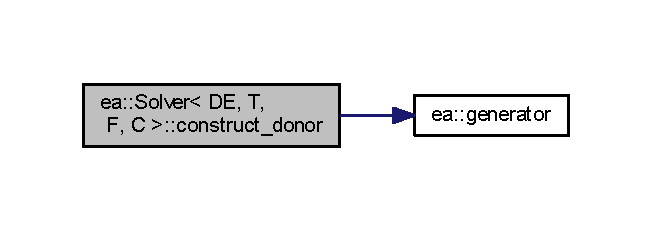
\includegraphics[width=313pt]{classea_1_1_solver_3_01_d_e_00_01_t_00_01_f_00_01_c_01_4_a69dabdddba116ddb5685355119bd77e0_cgraph}
\end{center}
\end{figure}
\mbox{\Hypertarget{classea_1_1_solver_3_01_d_e_00_01_t_00_01_f_00_01_c_01_4_a043f8134c53f09519283b8320d7a2ade}\label{classea_1_1_solver_3_01_d_e_00_01_t_00_01_f_00_01_c_01_4_a043f8134c53f09519283b8320d7a2ade}} 
\index{ea\+::\+Solver$<$ D\+E, T, F, C $>$@{ea\+::\+Solver$<$ D\+E, T, F, C $>$}!construct\+\_\+trial@{construct\+\_\+trial}}
\index{construct\+\_\+trial@{construct\+\_\+trial}!ea\+::\+Solver$<$ D\+E, T, F, C $>$@{ea\+::\+Solver$<$ D\+E, T, F, C $>$}}
\subsubsection{\texorpdfstring{construct\+\_\+trial()}{construct\_trial()}}
{\footnotesize\ttfamily template$<$typename T , typename F , typename C $>$ \\
std\+::vector$<$ T $>$ \hyperlink{classea_1_1_solver}{ea\+::\+Solver}$<$ \hyperlink{structea_1_1_d_e}{DE}, T, F, C $>$\+::construct\+\_\+trial (\begin{DoxyParamCaption}\item[{const std\+::vector$<$ T $>$ \&}]{target,  }\item[{const std\+::vector$<$ T $>$ \&}]{donor }\end{DoxyParamCaption})\hspace{0.3cm}{\ttfamily [private]}}



Method that constructs the trial vector. 


\begin{DoxyParams}{Parameters}
{\em target} & Target vector (an individual) \\
\hline
{\em donor} & Donor vector produced from \hyperlink{classea_1_1_solver_3_01_d_e_00_01_t_00_01_f_00_01_c_01_4_a69dabdddba116ddb5685355119bd77e0}{construct\+\_\+donor()} \\
\hline
\end{DoxyParams}
\begin{DoxyReturn}{Returns}
A trial vector that is compared with the current individual 
\end{DoxyReturn}


Definition at line 150 of file differentialevo.\+h.



References ea\+::generator().


\begin{DoxyCode}
151     \{
152         std::vector<T> trial(\hyperlink{classea_1_1_solver_3_01_d_e_00_01_t_00_01_f_00_01_c_01_4_a789b8665ce321248e3999907c37d0963}{de}.ndv);
153         std::vector<size\_t> j\_indices(\hyperlink{classea_1_1_solver_3_01_d_e_00_01_t_00_01_f_00_01_c_01_4_a789b8665ce321248e3999907c37d0963}{de}.ndv);
154         \textcolor{keywordflow}{for} (\textcolor{keywordtype}{size\_t} j = 0; j < \hyperlink{classea_1_1_solver_3_01_d_e_00_01_t_00_01_f_00_01_c_01_4_a789b8665ce321248e3999907c37d0963}{de}.ndv; ++j)
155         \{
156             j\_indices[j] = j;
157         \}
158         std::uniform\_int\_distribution<size\_t> j\_ind\_distribution(0, \hyperlink{classea_1_1_solver_3_01_d_e_00_01_t_00_01_f_00_01_c_01_4_a789b8665ce321248e3999907c37d0963}{de}.ndv - 1);
159         \textcolor{keywordflow}{for} (\textcolor{keywordtype}{size\_t} j = 0; j < \hyperlink{classea_1_1_solver_3_01_d_e_00_01_t_00_01_f_00_01_c_01_4_a789b8665ce321248e3999907c37d0963}{de}.ndv; ++j)
160         \{
161             \textcolor{keyword}{const} T& epsilon = this->\hyperlink{classea_1_1_solver__base_ae88f44b13e264e092d3bbaeca6b3bd19}{distribution}(\hyperlink{namespaceea_a385e8ca8ba4ae2f69dcfffa79f20c2ff}{generator});
162             \textcolor{keyword}{const} \textcolor{keywordtype}{size\_t}& jrand = j\_indices[j\_ind\_distribution(\hyperlink{namespaceea_a385e8ca8ba4ae2f69dcfffa79f20c2ff}{generator})];
163             \textcolor{keywordflow}{if} (epsilon <= \hyperlink{classea_1_1_solver_3_01_d_e_00_01_t_00_01_f_00_01_c_01_4_a789b8665ce321248e3999907c37d0963}{de}.cr || j == jrand)
164             \{
165                 trial[j] = donor[j];
166             \}
167             \textcolor{keywordflow}{else}
168             \{
169                 trial[j] = target[j];
170             \}
171         \}
172         \textcolor{keywordflow}{return} trial;
173     \}
\end{DoxyCode}
Here is the call graph for this function\+:
\nopagebreak
\begin{figure}[H]
\begin{center}
\leavevmode
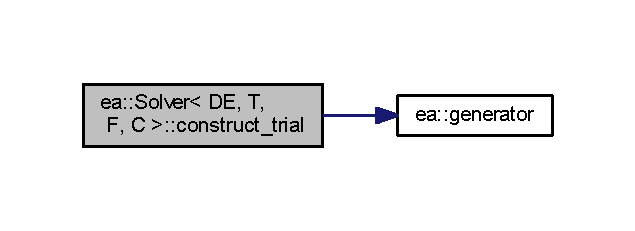
\includegraphics[width=305pt]{classea_1_1_solver_3_01_d_e_00_01_t_00_01_f_00_01_c_01_4_a043f8134c53f09519283b8320d7a2ade_cgraph}
\end{center}
\end{figure}
\mbox{\Hypertarget{classea_1_1_solver_3_01_d_e_00_01_t_00_01_f_00_01_c_01_4_a122c904c555a0be3b27160d6f883fd1b}\label{classea_1_1_solver_3_01_d_e_00_01_t_00_01_f_00_01_c_01_4_a122c904c555a0be3b27160d6f883fd1b}} 
\index{ea\+::\+Solver$<$ D\+E, T, F, C $>$@{ea\+::\+Solver$<$ D\+E, T, F, C $>$}!display\+\_\+parameters@{display\+\_\+parameters}}
\index{display\+\_\+parameters@{display\+\_\+parameters}!ea\+::\+Solver$<$ D\+E, T, F, C $>$@{ea\+::\+Solver$<$ D\+E, T, F, C $>$}}
\subsubsection{\texorpdfstring{display\+\_\+parameters()}{display\_parameters()}}
{\footnotesize\ttfamily template$<$typename T , typename F , typename C $>$ \\
\hyperlink{classea_1_1_solver}{ea\+::\+Solver}$<$ \hyperlink{structea_1_1_d_e}{DE}, T, F, C $>$\+::display\+\_\+parameters (\begin{DoxyParamCaption}{ }\end{DoxyParamCaption})\hspace{0.3cm}{\ttfamily [inline]}, {\ttfamily [private]}}



Display the parameters of \hyperlink{structea_1_1_d_e}{DE}. 

\begin{DoxyReturn}{Returns}
A std\+::stringstream of the parameters 
\end{DoxyReturn}


Definition at line 114 of file differentialevo.\+h.



References ea\+::\+D\+E$<$ T $>$\+::cr, and ea\+::\+D\+E$<$ T $>$\+::f\+\_\+param.


\begin{DoxyCode}
115         \{
116             std::stringstream parameters;
117             parameters << \textcolor{stringliteral}{"Crossover Rate:"} << \textcolor{stringliteral}{","} << \hyperlink{classea_1_1_solver_3_01_d_e_00_01_t_00_01_f_00_01_c_01_4_a789b8665ce321248e3999907c37d0963}{de}.cr << \textcolor{stringliteral}{","};
118             parameters << \textcolor{stringliteral}{"Mutation Scale Factor:"} << \textcolor{stringliteral}{","} << \hyperlink{classea_1_1_solver_3_01_d_e_00_01_t_00_01_f_00_01_c_01_4_a789b8665ce321248e3999907c37d0963}{de}.f\_param;
119             \textcolor{keywordflow}{return} parameters;
120         \}
\end{DoxyCode}
\mbox{\Hypertarget{classea_1_1_solver_3_01_d_e_00_01_t_00_01_f_00_01_c_01_4_a6e560e4d8fb8f578ebe0fd7beb802632}\label{classea_1_1_solver_3_01_d_e_00_01_t_00_01_f_00_01_c_01_4_a6e560e4d8fb8f578ebe0fd7beb802632}} 
\index{ea\+::\+Solver$<$ D\+E, T, F, C $>$@{ea\+::\+Solver$<$ D\+E, T, F, C $>$}!run\+\_\+algo@{run\+\_\+algo}}
\index{run\+\_\+algo@{run\+\_\+algo}!ea\+::\+Solver$<$ D\+E, T, F, C $>$@{ea\+::\+Solver$<$ D\+E, T, F, C $>$}}
\subsubsection{\texorpdfstring{run\+\_\+algo()}{run\_algo()}}
{\footnotesize\ttfamily template$<$typename T , typename F , typename C $>$ \\
void \hyperlink{classea_1_1_solver}{ea\+::\+Solver}$<$ \hyperlink{structea_1_1_d_e}{DE}, T, F, C $>$\+::run\+\_\+algo (\begin{DoxyParamCaption}{ }\end{DoxyParamCaption})\hspace{0.3cm}{\ttfamily [private]}}



Runs the algorithm until stopping criteria return void. 

Differential Evolution starts here

Construct donor and trial vectors

Recalculate minimum cost individual of the population

Stopping Criteria 

Definition at line 176 of file differentialevo.\+h.


\begin{DoxyCode}
177     \{
178         std::vector< std::vector<T> > personal\_best = this->\hyperlink{classea_1_1_solver__base_ad75bc440d24a46e97694c7c889f2ecde}{individuals};
180         \textcolor{keywordflow}{for} (\textcolor{keywordtype}{size\_t} iter = 0; iter < \hyperlink{classea_1_1_solver_3_01_d_e_00_01_t_00_01_f_00_01_c_01_4_a789b8665ce321248e3999907c37d0963}{de}.iter\_max; ++iter)
181         \{
182             \textcolor{keywordflow}{for} (\textcolor{keyword}{auto}& p : this->\hyperlink{classea_1_1_solver__base_ad75bc440d24a46e97694c7c889f2ecde}{individuals})
183             \{
185                 std::vector<T> donor = \hyperlink{classea_1_1_solver_3_01_d_e_00_01_t_00_01_f_00_01_c_01_4_a69dabdddba116ddb5685355119bd77e0}{construct\_donor}();
186                 \textcolor{keywordflow}{while} (!this->\hyperlink{classea_1_1_solver__base_a6914e89d30e7484f2b4af1783f0de8c3}{c}(donor))
187                 \{
188                     donor = \hyperlink{classea_1_1_solver_3_01_d_e_00_01_t_00_01_f_00_01_c_01_4_a69dabdddba116ddb5685355119bd77e0}{construct\_donor}();
189                 \}
190                 \textcolor{keyword}{const} std::vector<T>& trial = \hyperlink{classea_1_1_solver_3_01_d_e_00_01_t_00_01_f_00_01_c_01_4_a043f8134c53f09519283b8320d7a2ade}{construct\_trial}(p, donor);
191                 \textcolor{keywordflow}{if} (this->\hyperlink{classea_1_1_solver__base_ae0a893780c93dfe17c1d17301de6494f}{f}(trial) <= this->\hyperlink{classea_1_1_solver__base_ae0a893780c93dfe17c1d17301de6494f}{f}(p))
192                 \{
193                     p = trial;
194                 \}
195             \}
197             this->\hyperlink{classea_1_1_solver__base_ac69a6c714298054039acbbbf5d2eea23}{find\_min\_cost}();
199             this->\hyperlink{classea_1_1_solver__base_a8f9a321eb87e57636cf0b0f3a57b6fc2}{last\_iter} = iter;
200             \textcolor{keywordflow}{if} (\hyperlink{classea_1_1_solver_3_01_d_e_00_01_t_00_01_f_00_01_c_01_4_a789b8665ce321248e3999907c37d0963}{de}.tol > std::abs(this->f(this->min\_cost)))
201             \{
202                 this->\hyperlink{classea_1_1_solver__base_a1cdb824e8df6d4a8f228820ea85c9b05}{solved\_flag} = \textcolor{keyword}{true};
203                 \textcolor{keywordflow}{break};
204             \}
205         \}
206     \}
\end{DoxyCode}
\mbox{\Hypertarget{classea_1_1_solver_3_01_d_e_00_01_t_00_01_f_00_01_c_01_4_a86a25b0977865969248efd4e79e4982f}\label{classea_1_1_solver_3_01_d_e_00_01_t_00_01_f_00_01_c_01_4_a86a25b0977865969248efd4e79e4982f}} 
\index{ea\+::\+Solver$<$ D\+E, T, F, C $>$@{ea\+::\+Solver$<$ D\+E, T, F, C $>$}!set\+\_\+indices@{set\+\_\+indices}}
\index{set\+\_\+indices@{set\+\_\+indices}!ea\+::\+Solver$<$ D\+E, T, F, C $>$@{ea\+::\+Solver$<$ D\+E, T, F, C $>$}}
\subsubsection{\texorpdfstring{set\+\_\+indices()}{set\_indices()}}
{\footnotesize\ttfamily template$<$typename T , typename F , typename C $>$ \\
\hyperlink{classea_1_1_solver}{ea\+::\+Solver}$<$ \hyperlink{structea_1_1_d_e}{DE}, T, F, C $>$\+::set\+\_\+indices (\begin{DoxyParamCaption}{ }\end{DoxyParamCaption})\hspace{0.3cm}{\ttfamily [inline]}, {\ttfamily [private]}}



Generate the indices. 

\begin{DoxyReturn}{Returns}
The vector of the population indices 
\end{DoxyReturn}


Definition at line 101 of file differentialevo.\+h.



References ea\+::\+E\+A\+\_\+base$<$ T $>$\+::npop.


\begin{DoxyCode}
102         \{
103             std::vector<size\_t> \hyperlink{classea_1_1_solver_3_01_d_e_00_01_t_00_01_f_00_01_c_01_4_a8428ecceaab1c7e26715ed2f72654693}{indices};
104             \textcolor{keywordflow}{for} (\textcolor{keywordtype}{size\_t} i = 0; i < \hyperlink{classea_1_1_solver_3_01_d_e_00_01_t_00_01_f_00_01_c_01_4_a789b8665ce321248e3999907c37d0963}{de}.npop; ++i)
105             \{
106                 indices.push\_back(i);
107             \}
108             \textcolor{keywordflow}{return} \hyperlink{classea_1_1_solver_3_01_d_e_00_01_t_00_01_f_00_01_c_01_4_a8428ecceaab1c7e26715ed2f72654693}{indices};
109         \};
\end{DoxyCode}


\subsection{Friends And Related Function Documentation}
\mbox{\Hypertarget{classea_1_1_solver_3_01_d_e_00_01_t_00_01_f_00_01_c_01_4_af331e622818a725800b24cd03d46f3f1}\label{classea_1_1_solver_3_01_d_e_00_01_t_00_01_f_00_01_c_01_4_af331e622818a725800b24cd03d46f3f1}} 
\index{ea\+::\+Solver$<$ D\+E, T, F, C $>$@{ea\+::\+Solver$<$ D\+E, T, F, C $>$}!Solver\+\_\+base$<$ Solver$<$ D\+E, T, F, C $>$, D\+E, T, F, C $>$@{Solver\+\_\+base$<$ Solver$<$ D\+E, T, F, C $>$, D\+E, T, F, C $>$}}
\index{Solver\+\_\+base$<$ Solver$<$ D\+E, T, F, C $>$, D\+E, T, F, C $>$@{Solver\+\_\+base$<$ Solver$<$ D\+E, T, F, C $>$, D\+E, T, F, C $>$}!ea\+::\+Solver$<$ D\+E, T, F, C $>$@{ea\+::\+Solver$<$ D\+E, T, F, C $>$}}
\subsubsection{\texorpdfstring{Solver\+\_\+base$<$ Solver$<$ D\+E, T, F, C $>$, D\+E, T, F, C $>$}{Solver\_base< Solver< DE, T, F, C >, DE, T, F, C >}}
{\footnotesize\ttfamily template$<$typename T , typename F , typename C $>$ \\
friend class \hyperlink{classea_1_1_solver__base}{Solver\+\_\+base}$<$ \hyperlink{classea_1_1_solver}{Solver}$<$ \hyperlink{structea_1_1_d_e}{DE}, T, F, C $>$, \hyperlink{structea_1_1_d_e}{DE}, T, F, C $>$\hspace{0.3cm}{\ttfamily [friend]}}



Definition at line 63 of file differentialevo.\+h.



\subsection{Member Data Documentation}
\mbox{\Hypertarget{classea_1_1_solver_3_01_d_e_00_01_t_00_01_f_00_01_c_01_4_a789b8665ce321248e3999907c37d0963}\label{classea_1_1_solver_3_01_d_e_00_01_t_00_01_f_00_01_c_01_4_a789b8665ce321248e3999907c37d0963}} 
\index{ea\+::\+Solver$<$ D\+E, T, F, C $>$@{ea\+::\+Solver$<$ D\+E, T, F, C $>$}!de@{de}}
\index{de@{de}!ea\+::\+Solver$<$ D\+E, T, F, C $>$@{ea\+::\+Solver$<$ D\+E, T, F, C $>$}}
\subsubsection{\texorpdfstring{de}{de}}
{\footnotesize\ttfamily template$<$typename T , typename F , typename C $>$ \\
const \hyperlink{structea_1_1_d_e}{DE}$<$T$>$\& \hyperlink{classea_1_1_solver}{ea\+::\+Solver}$<$ \hyperlink{structea_1_1_d_e}{DE}, T, F, C $>$\+::de\hspace{0.3cm}{\ttfamily [private]}}



Differential Evolution structure used internally (reference to solver\+\_\+struct) 



Definition at line 77 of file differentialevo.\+h.

\mbox{\Hypertarget{classea_1_1_solver_3_01_d_e_00_01_t_00_01_f_00_01_c_01_4_a2f762378d566944899b2a07a5c74fc7f}\label{classea_1_1_solver_3_01_d_e_00_01_t_00_01_f_00_01_c_01_4_a2f762378d566944899b2a07a5c74fc7f}} 
\index{ea\+::\+Solver$<$ D\+E, T, F, C $>$@{ea\+::\+Solver$<$ D\+E, T, F, C $>$}!ind\+\_\+distribution@{ind\+\_\+distribution}}
\index{ind\+\_\+distribution@{ind\+\_\+distribution}!ea\+::\+Solver$<$ D\+E, T, F, C $>$@{ea\+::\+Solver$<$ D\+E, T, F, C $>$}}
\subsubsection{\texorpdfstring{ind\+\_\+distribution}{ind\_distribution}}
{\footnotesize\ttfamily template$<$typename T , typename F , typename C $>$ \\
std\+::uniform\+\_\+int\+\_\+distribution$<$size\+\_\+t$>$ \hyperlink{classea_1_1_solver}{ea\+::\+Solver}$<$ \hyperlink{structea_1_1_d_e}{DE}, T, F, C $>$\+::ind\+\_\+distribution\hspace{0.3cm}{\ttfamily [private]}}



Uniform size\+\_\+t distribution of the indices. 



Definition at line 84 of file differentialevo.\+h.

\mbox{\Hypertarget{classea_1_1_solver_3_01_d_e_00_01_t_00_01_f_00_01_c_01_4_a8428ecceaab1c7e26715ed2f72654693}\label{classea_1_1_solver_3_01_d_e_00_01_t_00_01_f_00_01_c_01_4_a8428ecceaab1c7e26715ed2f72654693}} 
\index{ea\+::\+Solver$<$ D\+E, T, F, C $>$@{ea\+::\+Solver$<$ D\+E, T, F, C $>$}!indices@{indices}}
\index{indices@{indices}!ea\+::\+Solver$<$ D\+E, T, F, C $>$@{ea\+::\+Solver$<$ D\+E, T, F, C $>$}}
\subsubsection{\texorpdfstring{indices}{indices}}
{\footnotesize\ttfamily template$<$typename T , typename F , typename C $>$ \\
const std\+::vector$<$size\+\_\+t$>$ \hyperlink{classea_1_1_solver}{ea\+::\+Solver}$<$ \hyperlink{structea_1_1_d_e}{DE}, T, F, C $>$\+::indices\hspace{0.3cm}{\ttfamily [private]}}



Indices of population. 



Definition at line 82 of file differentialevo.\+h.



The documentation for this class was generated from the following file\+:\begin{DoxyCompactItemize}
\item 
\hyperlink{differentialevo_8h}{differentialevo.\+h}\end{DoxyCompactItemize}

\hypertarget{classea_1_1_solver_3_01_g_a_00_01_t_00_01_f_00_01_c_01_4}{}\section{ea\+:\+:Solver$<$ GA, T, F, C $>$ Class Template Reference}
\label{classea_1_1_solver_3_01_g_a_00_01_t_00_01_f_00_01_c_01_4}\index{ea\+::\+Solver$<$ G\+A, T, F, C $>$@{ea\+::\+Solver$<$ G\+A, T, F, C $>$}}


Genetic Algorithms (\hyperlink{structea_1_1_g_a}{GA}) Class.  




{\ttfamily \#include $<$geneticalgo.\+h$>$}



Inheritance diagram for ea\+:\+:Solver$<$ GA, T, F, C $>$\+:
\nopagebreak
\begin{figure}[H]
\begin{center}
\leavevmode
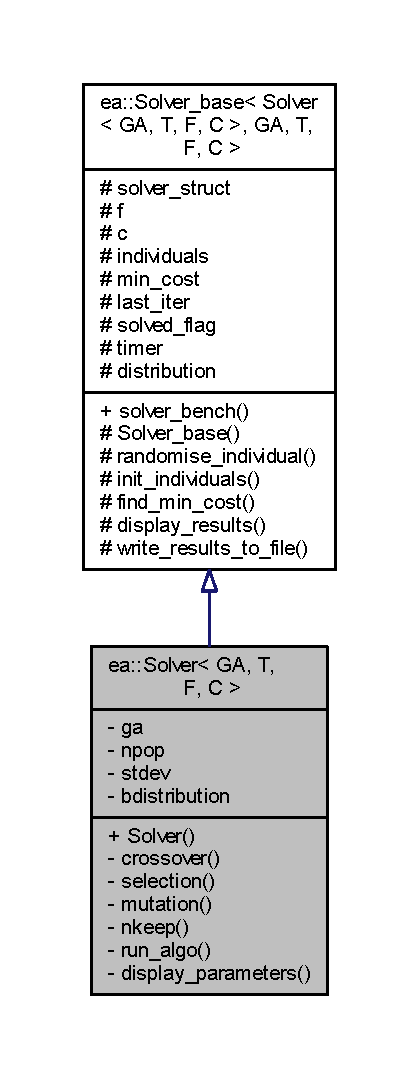
\includegraphics[width=201pt]{classea_1_1_solver_3_01_g_a_00_01_t_00_01_f_00_01_c_01_4__inherit__graph}
\end{center}
\end{figure}
\subsection*{Public Member Functions}
\begin{DoxyCompactItemize}
\item 
\hyperlink{classea_1_1_solver_3_01_g_a_00_01_t_00_01_f_00_01_c_01_4_a5c9e7819aa3d3a3ee99f67bc4a3aae5a}{Solver} (const \hyperlink{structea_1_1_g_a}{GA}$<$ T $>$ \&i\+\_\+ga, F \hyperlink{classea_1_1_solver__base_ae0a893780c93dfe17c1d17301de6494f}{f}, C \hyperlink{classea_1_1_solver__base_a6914e89d30e7484f2b4af1783f0de8c3}{c})
\begin{DoxyCompactList}\small\item\em Constructor. \end{DoxyCompactList}\end{DoxyCompactItemize}
\subsection*{Private Member Functions}
\begin{DoxyCompactItemize}
\item 
std\+::vector$<$ T $>$ \hyperlink{classea_1_1_solver_3_01_g_a_00_01_t_00_01_f_00_01_c_01_4_ad197350b0ef8bc73293fe31978702f02}{crossover} (std\+::vector$<$ T $>$ r, std\+::vector$<$ T $>$ s)
\begin{DoxyCompactList}\small\item\em Crossover step of \hyperlink{structea_1_1_g_a}{GA}. \end{DoxyCompactList}\item 
std\+::vector$<$ T $>$ \hyperlink{classea_1_1_solver_3_01_g_a_00_01_t_00_01_f_00_01_c_01_4_a1bc73c28211d7ba80665b286fbdea948}{selection} ()
\begin{DoxyCompactList}\small\item\em Selection step of \hyperlink{structea_1_1_g_a}{GA}. \end{DoxyCompactList}\item 
std\+::vector$<$ T $>$ \hyperlink{classea_1_1_solver_3_01_g_a_00_01_t_00_01_f_00_01_c_01_4_adde7de03b3c72d6b491a566699b6a4e4}{mutation} (const std\+::vector$<$ T $>$ \&individual)
\begin{DoxyCompactList}\small\item\em Mutation step of \hyperlink{structea_1_1_g_a}{GA}. \end{DoxyCompactList}\item 
size\+\_\+t \hyperlink{classea_1_1_solver_3_01_g_a_00_01_t_00_01_f_00_01_c_01_4_a42fe3561ccfab0dd666410e243d977e5}{nkeep} ()
\begin{DoxyCompactList}\small\item\em Returns number of individuals to be kept in each generation. \end{DoxyCompactList}\item 
void \hyperlink{classea_1_1_solver_3_01_g_a_00_01_t_00_01_f_00_01_c_01_4_aa03709c3636280a24879d01f9ad128ea}{run\+\_\+algo} ()
\begin{DoxyCompactList}\small\item\em Runs the algorithm until stopping criteria return void. \end{DoxyCompactList}\item 
std\+::stringstream \hyperlink{classea_1_1_solver_3_01_g_a_00_01_t_00_01_f_00_01_c_01_4_a36b4364bdb9a079aa327d6664d538167}{display\+\_\+parameters} ()
\begin{DoxyCompactList}\small\item\em Display the parameters of \hyperlink{structea_1_1_g_a}{GA}. \end{DoxyCompactList}\end{DoxyCompactItemize}
\subsection*{Private Attributes}
\begin{DoxyCompactItemize}
\item 
const \hyperlink{structea_1_1_g_a}{GA}$<$ T $>$ \& \hyperlink{classea_1_1_solver_3_01_g_a_00_01_t_00_01_f_00_01_c_01_4_a5e56c4d15894af96c2be5fcaec7d14fb}{ga}
\begin{DoxyCompactList}\small\item\em Genetic Algorithms structure used internally (reference to solver\+\_\+struct) \end{DoxyCompactList}\item 
size\+\_\+t \hyperlink{classea_1_1_solver_3_01_g_a_00_01_t_00_01_f_00_01_c_01_4_a805f49211363542de6984c7fd2c97c9c}{npop}
\begin{DoxyCompactList}\small\item\em Size of the population is mutable. \end{DoxyCompactList}\item 
std\+::vector$<$ T $>$ \hyperlink{classea_1_1_solver_3_01_g_a_00_01_t_00_01_f_00_01_c_01_4_a097a7ec4bbcf9e5bade6e498d55d4d11}{stdev}
\begin{DoxyCompactList}\small\item\em Standard deviation is mutable, so a copy is created. \end{DoxyCompactList}\item 
boost\+::math\+::beta\+\_\+distribution$<$ T $>$ \hyperlink{classea_1_1_solver_3_01_g_a_00_01_t_00_01_f_00_01_c_01_4_a01dbd57c74c1ebd73e4ac976e29ecb33}{bdistribution}
\begin{DoxyCompactList}\small\item\em Beta distribution. \end{DoxyCompactList}\end{DoxyCompactItemize}
\subsection*{Friends}
\begin{DoxyCompactItemize}
\item 
class \hyperlink{classea_1_1_solver_3_01_g_a_00_01_t_00_01_f_00_01_c_01_4_a36e0662bcb575fd6a11cec4eedf85117}{Solver\+\_\+base$<$ Solver$<$ G\+A, T, F, C $>$, G\+A, T, F, C $>$}
\end{DoxyCompactItemize}
\subsection*{Additional Inherited Members}


\subsection{Detailed Description}
\subsubsection*{template$<$typename T, typename F, typename C$>$\newline
class ea\+::\+Solver$<$ G\+A, T, F, C $>$}

Genetic Algorithms (\hyperlink{structea_1_1_g_a}{GA}) Class. 

Definition at line 73 of file geneticalgo.\+h.



\subsection{Constructor \& Destructor Documentation}
\mbox{\Hypertarget{classea_1_1_solver_3_01_g_a_00_01_t_00_01_f_00_01_c_01_4_a5c9e7819aa3d3a3ee99f67bc4a3aae5a}\label{classea_1_1_solver_3_01_g_a_00_01_t_00_01_f_00_01_c_01_4_a5c9e7819aa3d3a3ee99f67bc4a3aae5a}} 
\index{ea\+::\+Solver$<$ G\+A, T, F, C $>$@{ea\+::\+Solver$<$ G\+A, T, F, C $>$}!Solver@{Solver}}
\index{Solver@{Solver}!ea\+::\+Solver$<$ G\+A, T, F, C $>$@{ea\+::\+Solver$<$ G\+A, T, F, C $>$}}
\subsubsection{\texorpdfstring{Solver()}{Solver()}}
{\footnotesize\ttfamily template$<$typename T , typename F , typename C $>$ \\
\hyperlink{classea_1_1_solver}{ea\+::\+Solver}$<$ \hyperlink{structea_1_1_g_a}{GA}, T, F, C $>$\+::\hyperlink{classea_1_1_solver}{Solver} (\begin{DoxyParamCaption}\item[{const \hyperlink{structea_1_1_g_a}{GA}$<$ T $>$ \&}]{i\+\_\+ga,  }\item[{F}]{f,  }\item[{C}]{c }\end{DoxyParamCaption})\hspace{0.3cm}{\ttfamily [inline]}}



Constructor. 


\begin{DoxyParams}{Parameters}
{\em i\+\_\+ga} & The genetic algorithms parameter structure that is used to construct the solver \\
\hline
{\em f} & A reference to the objective function \\
\hline
{\em c} & A reference to the constraints function \\
\hline
\end{DoxyParams}
\begin{DoxyReturn}{Returns}
A \hyperlink{classea_1_1_solver_3_01_g_a_00_01_t_00_01_f_00_01_c_01_4}{Solver$<$\+G\+A, T, F, C$>$} object 
\end{DoxyReturn}


Definition at line 84 of file geneticalgo.\+h.


\begin{DoxyCode}
84                                             :
85             Solver\_base<Solver<GA, T, F, C>, GA, T, F, C> ( i\_ga, \hyperlink{classea_1_1_solver__base_ae0a893780c93dfe17c1d17301de6494f}{f}, \hyperlink{classea_1_1_solver__base_a6914e89d30e7484f2b4af1783f0de8c3}{c} ), 
86             \hyperlink{classea_1_1_solver_3_01_g_a_00_01_t_00_01_f_00_01_c_01_4_a5e56c4d15894af96c2be5fcaec7d14fb}{ga} ( this->\hyperlink{classea_1_1_solver__base_a5e1d821809f2d26c6f882942ad728127}{solver\_struct} ),
87             \hyperlink{classea_1_1_solver_3_01_g_a_00_01_t_00_01_f_00_01_c_01_4_a805f49211363542de6984c7fd2c97c9c}{npop} ( i\_ga.npop ),
88             \hyperlink{classea_1_1_solver_3_01_g_a_00_01_t_00_01_f_00_01_c_01_4_a097a7ec4bbcf9e5bade6e498d55d4d11}{stdev} ( i\_ga.stdev ),
89             \hyperlink{classea_1_1_solver_3_01_g_a_00_01_t_00_01_f_00_01_c_01_4_a01dbd57c74c1ebd73e4ac976e29ecb33}{bdistribution} (boost::math::beta\_distribution<T>(1, \hyperlink{classea_1_1_solver_3_01_g_a_00_01_t_00_01_f_00_01_c_01_4_a5e56c4d15894af96c2be5fcaec7d14fb}{ga}.alpha))
90         \{
91         \}
\end{DoxyCode}


\subsection{Member Function Documentation}
\mbox{\Hypertarget{classea_1_1_solver_3_01_g_a_00_01_t_00_01_f_00_01_c_01_4_ad197350b0ef8bc73293fe31978702f02}\label{classea_1_1_solver_3_01_g_a_00_01_t_00_01_f_00_01_c_01_4_ad197350b0ef8bc73293fe31978702f02}} 
\index{ea\+::\+Solver$<$ G\+A, T, F, C $>$@{ea\+::\+Solver$<$ G\+A, T, F, C $>$}!crossover@{crossover}}
\index{crossover@{crossover}!ea\+::\+Solver$<$ G\+A, T, F, C $>$@{ea\+::\+Solver$<$ G\+A, T, F, C $>$}}
\subsubsection{\texorpdfstring{crossover()}{crossover()}}
{\footnotesize\ttfamily template$<$typename T , typename F , typename C $>$ \\
std\+::vector$<$ T $>$ \hyperlink{classea_1_1_solver}{ea\+::\+Solver}$<$ \hyperlink{structea_1_1_g_a}{GA}, T, F, C $>$\+::crossover (\begin{DoxyParamCaption}\item[{std\+::vector$<$ T $>$}]{r,  }\item[{std\+::vector$<$ T $>$}]{s }\end{DoxyParamCaption})\hspace{0.3cm}{\ttfamily [private]}}



Crossover step of \hyperlink{structea_1_1_g_a}{GA}. 


\begin{DoxyParams}{Parameters}
{\em r,s} & Parent individuals \\
\hline
\end{DoxyParams}
\begin{DoxyReturn}{Returns}
An offspring from the two parents r and s 
\end{DoxyReturn}


Definition at line 152 of file geneticalgo.\+h.



References ea\+::generator().


\begin{DoxyCode}
153     \{
154         std::vector<T> offspring(\hyperlink{classea_1_1_solver_3_01_g_a_00_01_t_00_01_f_00_01_c_01_4_a5e56c4d15894af96c2be5fcaec7d14fb}{ga}.ndv);
155         std::vector<T> psi(\hyperlink{classea_1_1_solver_3_01_g_a_00_01_t_00_01_f_00_01_c_01_4_a5e56c4d15894af96c2be5fcaec7d14fb}{ga}.ndv);
156         \textcolor{keywordflow}{for} (\textcolor{keywordtype}{size\_t} j = 0; j < \hyperlink{classea_1_1_solver_3_01_g_a_00_01_t_00_01_f_00_01_c_01_4_a5e56c4d15894af96c2be5fcaec7d14fb}{ga}.ndv; ++j)
157         \{
158             psi[j] = this->\hyperlink{classea_1_1_solver__base_ae88f44b13e264e092d3bbaeca6b3bd19}{distribution}(\hyperlink{namespaceea_a385e8ca8ba4ae2f69dcfffa79f20c2ff}{generator});
159             offspring[j] = psi[j] * r[j] + (1 - psi[j]) * s[j];
160         \}
161         \textcolor{keywordflow}{return} offspring;
162     \}
\end{DoxyCode}
Here is the call graph for this function\+:
\nopagebreak
\begin{figure}[H]
\begin{center}
\leavevmode
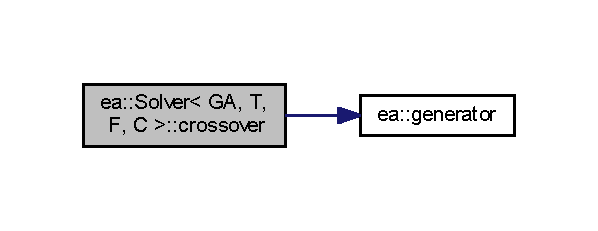
\includegraphics[width=287pt]{classea_1_1_solver_3_01_g_a_00_01_t_00_01_f_00_01_c_01_4_ad197350b0ef8bc73293fe31978702f02_cgraph}
\end{center}
\end{figure}
\mbox{\Hypertarget{classea_1_1_solver_3_01_g_a_00_01_t_00_01_f_00_01_c_01_4_a36b4364bdb9a079aa327d6664d538167}\label{classea_1_1_solver_3_01_g_a_00_01_t_00_01_f_00_01_c_01_4_a36b4364bdb9a079aa327d6664d538167}} 
\index{ea\+::\+Solver$<$ G\+A, T, F, C $>$@{ea\+::\+Solver$<$ G\+A, T, F, C $>$}!display\+\_\+parameters@{display\+\_\+parameters}}
\index{display\+\_\+parameters@{display\+\_\+parameters}!ea\+::\+Solver$<$ G\+A, T, F, C $>$@{ea\+::\+Solver$<$ G\+A, T, F, C $>$}}
\subsubsection{\texorpdfstring{display\+\_\+parameters()}{display\_parameters()}}
{\footnotesize\ttfamily template$<$typename T , typename F , typename C $>$ \\
\hyperlink{classea_1_1_solver}{ea\+::\+Solver}$<$ \hyperlink{structea_1_1_g_a}{GA}, T, F, C $>$\+::display\+\_\+parameters (\begin{DoxyParamCaption}{ }\end{DoxyParamCaption})\hspace{0.3cm}{\ttfamily [inline]}, {\ttfamily [private]}}



Display the parameters of \hyperlink{structea_1_1_g_a}{GA}. 

\begin{DoxyReturn}{Returns}
A std\+::stringstream of the parameters 
\end{DoxyReturn}


Definition at line 133 of file geneticalgo.\+h.



References ea\+::\+G\+A$<$ T $>$\+::alpha, ea\+::keep\+\_\+same, ea\+::\+G\+A$<$ T $>$\+::pi, ea\+::re\+\_\+mutate, ea\+::remove, ea\+::\+G\+A$<$ T $>$\+::strategy, and ea\+::\+G\+A$<$ T $>$\+::x\+\_\+rate.


\begin{DoxyCode}
134         \{
135             std::stringstream parameters;
136             parameters << \textcolor{stringliteral}{"Natural Selection Rate:"} << \textcolor{stringliteral}{","} << \hyperlink{classea_1_1_solver_3_01_g_a_00_01_t_00_01_f_00_01_c_01_4_a5e56c4d15894af96c2be5fcaec7d14fb}{ga}.x\_rate << \textcolor{stringliteral}{","};
137             parameters << \textcolor{stringliteral}{"Probability of Mutation:"} << \textcolor{stringliteral}{","} << \hyperlink{classea_1_1_solver_3_01_g_a_00_01_t_00_01_f_00_01_c_01_4_a5e56c4d15894af96c2be5fcaec7d14fb}{ga}.pi << \textcolor{stringliteral}{","};
138             parameters << \textcolor{stringliteral}{"Beta Distribution alpha:"} << \textcolor{stringliteral}{","} << \hyperlink{classea_1_1_solver_3_01_g_a_00_01_t_00_01_f_00_01_c_01_4_a5e56c4d15894af96c2be5fcaec7d14fb}{ga}.alpha << \textcolor{stringliteral}{","};
139             parameters << \textcolor{stringliteral}{"Strategy:"} << \textcolor{stringliteral}{","};
140             \textcolor{keywordflow}{switch} (\hyperlink{classea_1_1_solver_3_01_g_a_00_01_t_00_01_f_00_01_c_01_4_a5e56c4d15894af96c2be5fcaec7d14fb}{ga}.strategy)
141             \{
142             \textcolor{keywordflow}{case} \hyperlink{namespaceea_a8e369877773b4db67b8512efdb4f8f89ac4a301043ce8554dfced7a0c0698bdad}{Strategy::keep\_same}: parameters << \textcolor{stringliteral}{"Keep same individual"}; \textcolor{keywordflow}{break};
143             \textcolor{keywordflow}{case} \hyperlink{namespaceea_a8e369877773b4db67b8512efdb4f8f89a49a303c9c8d8a0c15a7fc97cd4b1db0d}{Strategy::re\_mutate}: parameters << \textcolor{stringliteral}{"Re-mutate individual"}; \textcolor{keywordflow}{break};
144             \textcolor{keywordflow}{case} \hyperlink{namespaceea_a8e369877773b4db67b8512efdb4f8f89a0f6969d7052da9261e31ddb6e88c136e}{Strategy::remove}: parameters << \textcolor{stringliteral}{"Remove individual"}; \textcolor{keywordflow}{break};
145             \textcolor{keywordflow}{default}: parameters << \textcolor{stringliteral}{"Do nothing"}; \textcolor{keywordflow}{break};
146             \}
147             \textcolor{keywordflow}{return} parameters;
148         \}
\end{DoxyCode}
\mbox{\Hypertarget{classea_1_1_solver_3_01_g_a_00_01_t_00_01_f_00_01_c_01_4_adde7de03b3c72d6b491a566699b6a4e4}\label{classea_1_1_solver_3_01_g_a_00_01_t_00_01_f_00_01_c_01_4_adde7de03b3c72d6b491a566699b6a4e4}} 
\index{ea\+::\+Solver$<$ G\+A, T, F, C $>$@{ea\+::\+Solver$<$ G\+A, T, F, C $>$}!mutation@{mutation}}
\index{mutation@{mutation}!ea\+::\+Solver$<$ G\+A, T, F, C $>$@{ea\+::\+Solver$<$ G\+A, T, F, C $>$}}
\subsubsection{\texorpdfstring{mutation()}{mutation()}}
{\footnotesize\ttfamily template$<$typename T , typename F , typename C $>$ \\
std\+::vector$<$ T $>$ \hyperlink{classea_1_1_solver}{ea\+::\+Solver}$<$ \hyperlink{structea_1_1_g_a}{GA}, T, F, C $>$\+::mutation (\begin{DoxyParamCaption}\item[{const std\+::vector$<$ T $>$ \&}]{individual }\end{DoxyParamCaption})\hspace{0.3cm}{\ttfamily [private]}}



Mutation step of \hyperlink{structea_1_1_g_a}{GA}. 


\begin{DoxyParams}{Parameters}
{\em individual} & An individual of the population \\
\hline
\end{DoxyParams}
\begin{DoxyReturn}{Returns}
A mutated individual 
\end{DoxyReturn}


Definition at line 178 of file geneticalgo.\+h.



References ea\+::generator().


\begin{DoxyCode}
179     \{
180         std::vector<T> mutated = individual;
181         \textcolor{keywordflow}{for} (\textcolor{keywordtype}{size\_t} j = 0; j < \hyperlink{classea_1_1_solver_3_01_g_a_00_01_t_00_01_f_00_01_c_01_4_a5e56c4d15894af96c2be5fcaec7d14fb}{ga}.ndv; ++j)
182         \{
183             \textcolor{keyword}{const} T r = this->\hyperlink{classea_1_1_solver__base_ae88f44b13e264e092d3bbaeca6b3bd19}{distribution}(\hyperlink{namespaceea_a385e8ca8ba4ae2f69dcfffa79f20c2ff}{generator});
184             \textcolor{keywordflow}{if} (\hyperlink{classea_1_1_solver_3_01_g_a_00_01_t_00_01_f_00_01_c_01_4_a5e56c4d15894af96c2be5fcaec7d14fb}{ga}.pi < r)
185             \{
186                 std::normal\_distribution<T> ndistribution(0, \hyperlink{classea_1_1_solver_3_01_g_a_00_01_t_00_01_f_00_01_c_01_4_a097a7ec4bbcf9e5bade6e498d55d4d11}{stdev}[j]);
187                 T epsilon = ndistribution(\hyperlink{namespaceea_a385e8ca8ba4ae2f69dcfffa79f20c2ff}{generator});
188                 mutated[j] = mutated[j] + epsilon;
189             \}
190         \}
191         \textcolor{keywordflow}{return} mutated;
192     \}
\end{DoxyCode}
Here is the call graph for this function\+:
\nopagebreak
\begin{figure}[H]
\begin{center}
\leavevmode
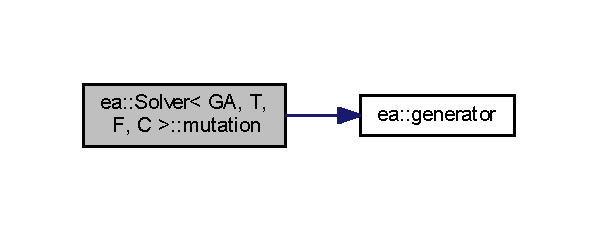
\includegraphics[width=287pt]{classea_1_1_solver_3_01_g_a_00_01_t_00_01_f_00_01_c_01_4_adde7de03b3c72d6b491a566699b6a4e4_cgraph}
\end{center}
\end{figure}
\mbox{\Hypertarget{classea_1_1_solver_3_01_g_a_00_01_t_00_01_f_00_01_c_01_4_a42fe3561ccfab0dd666410e243d977e5}\label{classea_1_1_solver_3_01_g_a_00_01_t_00_01_f_00_01_c_01_4_a42fe3561ccfab0dd666410e243d977e5}} 
\index{ea\+::\+Solver$<$ G\+A, T, F, C $>$@{ea\+::\+Solver$<$ G\+A, T, F, C $>$}!nkeep@{nkeep}}
\index{nkeep@{nkeep}!ea\+::\+Solver$<$ G\+A, T, F, C $>$@{ea\+::\+Solver$<$ G\+A, T, F, C $>$}}
\subsubsection{\texorpdfstring{nkeep()}{nkeep()}}
{\footnotesize\ttfamily template$<$typename T , typename F , typename C $>$ \\
size\+\_\+t \hyperlink{classea_1_1_solver}{ea\+::\+Solver}$<$ \hyperlink{structea_1_1_g_a}{GA}, T, F, C $>$\+::nkeep (\begin{DoxyParamCaption}{ }\end{DoxyParamCaption})\hspace{0.3cm}{\ttfamily [private]}}



Returns number of individuals to be kept in each generation. 

\begin{DoxyReturn}{Returns}
The new nkeep 
\end{DoxyReturn}


Definition at line 195 of file geneticalgo.\+h.


\begin{DoxyCode}
196     \{
197         \textcolor{keywordflow}{return} \textcolor{keyword}{static\_cast<}\textcolor{keywordtype}{size\_t}\textcolor{keyword}{>}(std::ceil(static\_cast<T>(\hyperlink{classea_1_1_solver_3_01_g_a_00_01_t_00_01_f_00_01_c_01_4_a805f49211363542de6984c7fd2c97c9c}{npop}) * \hyperlink{classea_1_1_solver_3_01_g_a_00_01_t_00_01_f_00_01_c_01_4_a5e56c4d15894af96c2be5fcaec7d14fb}{ga}.x\_rate));
198     \}
\end{DoxyCode}
\mbox{\Hypertarget{classea_1_1_solver_3_01_g_a_00_01_t_00_01_f_00_01_c_01_4_aa03709c3636280a24879d01f9ad128ea}\label{classea_1_1_solver_3_01_g_a_00_01_t_00_01_f_00_01_c_01_4_aa03709c3636280a24879d01f9ad128ea}} 
\index{ea\+::\+Solver$<$ G\+A, T, F, C $>$@{ea\+::\+Solver$<$ G\+A, T, F, C $>$}!run\+\_\+algo@{run\+\_\+algo}}
\index{run\+\_\+algo@{run\+\_\+algo}!ea\+::\+Solver$<$ G\+A, T, F, C $>$@{ea\+::\+Solver$<$ G\+A, T, F, C $>$}}
\subsubsection{\texorpdfstring{run\+\_\+algo()}{run\_algo()}}
{\footnotesize\ttfamily template$<$typename T , typename F , typename C $>$ \\
void \hyperlink{classea_1_1_solver}{ea\+::\+Solver}$<$ \hyperlink{structea_1_1_g_a}{GA}, T, F, C $>$\+::run\+\_\+algo (\begin{DoxyParamCaption}{ }\end{DoxyParamCaption})\hspace{0.3cm}{\ttfamily [private]}}



Runs the algorithm until stopping criteria return void. 

Set the new population size which is previous population size + natural selection rate $\ast$ population size

Standard Deviation is not constant in \hyperlink{structea_1_1_g_a}{GA} 

Definition at line 201 of file geneticalgo.\+h.



References ea\+::keep\+\_\+same, ea\+::none, ea\+::re\+\_\+mutate, and ea\+::remove.


\begin{DoxyCode}
202     \{
203         \textcolor{keyword}{auto} comparator = [&](\textcolor{keyword}{const} std::vector<T>& l, \textcolor{keyword}{const} std::vector<T>& r)
204         \{
205             \textcolor{keywordflow}{return} this->\hyperlink{classea_1_1_solver__base_ae0a893780c93dfe17c1d17301de6494f}{f}(l) < this->\hyperlink{classea_1_1_solver__base_ae0a893780c93dfe17c1d17301de6494f}{f}(r);
206         \};
207         \textcolor{keywordflow}{for} (\textcolor{keywordtype}{size\_t} iter = 0; iter < \hyperlink{classea_1_1_solver_3_01_g_a_00_01_t_00_01_f_00_01_c_01_4_a5e56c4d15894af96c2be5fcaec7d14fb}{ga}.iter\_max; ++iter)
208         \{
210             \hyperlink{classea_1_1_solver_3_01_g_a_00_01_t_00_01_f_00_01_c_01_4_a805f49211363542de6984c7fd2c97c9c}{npop} = this->\hyperlink{classea_1_1_solver__base_ad75bc440d24a46e97694c7c889f2ecde}{individuals}.size();
211             std::sort(this->\hyperlink{classea_1_1_solver__base_ad75bc440d24a46e97694c7c889f2ecde}{individuals}.begin(), this->\hyperlink{classea_1_1_solver__base_ad75bc440d24a46e97694c7c889f2ecde}{individuals}.end(), comparator)
      ;
212             this->\hyperlink{classea_1_1_solver__base_ad75bc440d24a46e97694c7c889f2ecde}{individuals}.erase(this->\hyperlink{classea_1_1_solver__base_ad75bc440d24a46e97694c7c889f2ecde}{individuals}.begin() + 
      \hyperlink{classea_1_1_solver_3_01_g_a_00_01_t_00_01_f_00_01_c_01_4_a42fe3561ccfab0dd666410e243d977e5}{nkeep}(), this->\hyperlink{classea_1_1_solver__base_ad75bc440d24a46e97694c7c889f2ecde}{individuals}.begin() + this->\hyperlink{classea_1_1_solver__base_ad75bc440d24a46e97694c7c889f2ecde}{individuals}.size());
213             this->\hyperlink{classea_1_1_solver__base_af745cded954be26280d842c1e7c7f989}{min\_cost} = this->\hyperlink{classea_1_1_solver__base_ad75bc440d24a46e97694c7c889f2ecde}{individuals}[0];
214             this->\hyperlink{classea_1_1_solver__base_a8f9a321eb87e57636cf0b0f3a57b6fc2}{last\_iter} = iter;
215             \textcolor{keywordflow}{if} (\hyperlink{classea_1_1_solver_3_01_g_a_00_01_t_00_01_f_00_01_c_01_4_a5e56c4d15894af96c2be5fcaec7d14fb}{ga}.tol > std::abs(this->f(this->min\_cost)))
216             \{
217                 this->\hyperlink{classea_1_1_solver__base_a1cdb824e8df6d4a8f228820ea85c9b05}{solved\_flag} = \textcolor{keyword}{true};
218                 \textcolor{keywordflow}{break};
219             \}
220             \textcolor{keywordflow}{for} (\textcolor{keywordtype}{size\_t} i = 0; i < \hyperlink{classea_1_1_solver_3_01_g_a_00_01_t_00_01_f_00_01_c_01_4_a805f49211363542de6984c7fd2c97c9c}{npop}; ++i)
221             \{
222                 std::vector<T> offspring = \hyperlink{classea_1_1_solver_3_01_g_a_00_01_t_00_01_f_00_01_c_01_4_a1bc73c28211d7ba80665b286fbdea948}{selection}();
223                 this->\hyperlink{classea_1_1_solver__base_ad75bc440d24a46e97694c7c889f2ecde}{individuals}.push\_back(offspring);
224             \}
225             \textcolor{keywordflow}{if} (this->\hyperlink{classea_1_1_solver__base_ad75bc440d24a46e97694c7c889f2ecde}{individuals}.size() > 1000)
226             \{
227                 \textcolor{comment}{//this->individuals.erase(this->individuals.begin() + 1000, this->individuals.begin() +
       this->individuals.size());}
228             \}
229             \textcolor{keywordflow}{for} (\textcolor{keywordtype}{size\_t} i = 1; i < this->\hyperlink{classea_1_1_solver__base_ad75bc440d24a46e97694c7c889f2ecde}{individuals}.size(); ++i)
230             \{
231                 std::vector<T> mutated = \hyperlink{classea_1_1_solver_3_01_g_a_00_01_t_00_01_f_00_01_c_01_4_adde7de03b3c72d6b491a566699b6a4e4}{mutation}(this->\hyperlink{classea_1_1_solver__base_ad75bc440d24a46e97694c7c889f2ecde}{individuals}[i]);
232                 \textcolor{keywordflow}{if} (!this->\hyperlink{classea_1_1_solver__base_a6914e89d30e7484f2b4af1783f0de8c3}{c}(mutated))
233                 \{
234                     \textcolor{keywordflow}{switch} (\hyperlink{classea_1_1_solver_3_01_g_a_00_01_t_00_01_f_00_01_c_01_4_a5e56c4d15894af96c2be5fcaec7d14fb}{ga}.strategy)
235                     \{
236                     \textcolor{keywordflow}{case} \hyperlink{namespaceea_a8e369877773b4db67b8512efdb4f8f89ac4a301043ce8554dfced7a0c0698bdad}{Strategy::keep\_same}: this->
      \hyperlink{classea_1_1_solver__base_ad75bc440d24a46e97694c7c889f2ecde}{individuals}[i] = this->\hyperlink{classea_1_1_solver__base_ad75bc440d24a46e97694c7c889f2ecde}{individuals}[i]; \textcolor{keywordflow}{break};
237                     \textcolor{keywordflow}{case} \hyperlink{namespaceea_a8e369877773b4db67b8512efdb4f8f89a49a303c9c8d8a0c15a7fc97cd4b1db0d}{Strategy::re\_mutate}: 
238                     \{
239                         \textcolor{keywordflow}{while} (!this->\hyperlink{classea_1_1_solver__base_a6914e89d30e7484f2b4af1783f0de8c3}{c}(mutated))
240                         \{
241                             mutated = \hyperlink{classea_1_1_solver_3_01_g_a_00_01_t_00_01_f_00_01_c_01_4_adde7de03b3c72d6b491a566699b6a4e4}{mutation}(this->\hyperlink{classea_1_1_solver__base_ad75bc440d24a46e97694c7c889f2ecde}{individuals}[i]);
242                         \}
243                         \textcolor{keywordflow}{break};
244                         this->\hyperlink{classea_1_1_solver__base_ad75bc440d24a46e97694c7c889f2ecde}{individuals}[i] = mutated;
245                     \}
246                     \textcolor{keywordflow}{case} \hyperlink{namespaceea_a8e369877773b4db67b8512efdb4f8f89a0f6969d7052da9261e31ddb6e88c136e}{Strategy::remove}:
247                     \{
248                         \textcolor{keywordflow}{if} (i == this->\hyperlink{classea_1_1_solver__base_ad75bc440d24a46e97694c7c889f2ecde}{individuals}.size() - 1)
249                         \{
250                             this->\hyperlink{classea_1_1_solver__base_ad75bc440d24a46e97694c7c889f2ecde}{individuals}.pop\_back();
251                         \}
252                         \textcolor{keywordflow}{else}
253                         \{
254                             this->\hyperlink{classea_1_1_solver__base_ad75bc440d24a46e97694c7c889f2ecde}{individuals}.erase(this->\hyperlink{classea_1_1_solver__base_ad75bc440d24a46e97694c7c889f2ecde}{individuals}.begin() + i, 
      this->\hyperlink{classea_1_1_solver__base_ad75bc440d24a46e97694c7c889f2ecde}{individuals}.begin() + i + 1);
255                         \}
256                         \textcolor{keywordflow}{break};
257                     \}
258                     \textcolor{keywordflow}{case} \hyperlink{namespaceea_a8e369877773b4db67b8512efdb4f8f89a334c4a4c42fdb79d7ebc3e73b517e6f8}{Strategy::none}: \textcolor{keywordflow}{break};
259                     \textcolor{keywordflow}{default}: std::abort();
260                     \}
261                 \}
262                 \textcolor{keywordflow}{else}
263                 \{
264                     this->\hyperlink{classea_1_1_solver__base_ad75bc440d24a46e97694c7c889f2ecde}{individuals}[i] = mutated;
265                 \}
266             \}
268             \textcolor{keywordflow}{for} (\textcolor{keyword}{auto}& p : \hyperlink{classea_1_1_solver_3_01_g_a_00_01_t_00_01_f_00_01_c_01_4_a097a7ec4bbcf9e5bade6e498d55d4d11}{stdev})
269             \{
270                 p = p + 0.02 * p;
271             \}
272         \}
273     \}
\end{DoxyCode}
\mbox{\Hypertarget{classea_1_1_solver_3_01_g_a_00_01_t_00_01_f_00_01_c_01_4_a1bc73c28211d7ba80665b286fbdea948}\label{classea_1_1_solver_3_01_g_a_00_01_t_00_01_f_00_01_c_01_4_a1bc73c28211d7ba80665b286fbdea948}} 
\index{ea\+::\+Solver$<$ G\+A, T, F, C $>$@{ea\+::\+Solver$<$ G\+A, T, F, C $>$}!selection@{selection}}
\index{selection@{selection}!ea\+::\+Solver$<$ G\+A, T, F, C $>$@{ea\+::\+Solver$<$ G\+A, T, F, C $>$}}
\subsubsection{\texorpdfstring{selection()}{selection()}}
{\footnotesize\ttfamily template$<$typename T , typename F , typename C $>$ \\
std\+::vector$<$ T $>$ \hyperlink{classea_1_1_solver}{ea\+::\+Solver}$<$ \hyperlink{structea_1_1_g_a}{GA}, T, F, C $>$\+::selection (\begin{DoxyParamCaption}{ }\end{DoxyParamCaption})\hspace{0.3cm}{\ttfamily [private]}}



Selection step of \hyperlink{structea_1_1_g_a}{GA}. 

Select two parents r and s using a Beta distribution and generates an offspring using the crossover method \begin{DoxyReturn}{Returns}
An offspring from the two parents 
\end{DoxyReturn}
Generate r and s indices

Produce offsrping using r and s indices by crossover 

Definition at line 165 of file geneticalgo.\+h.



References ea\+::generator().


\begin{DoxyCode}
166     \{
168         T xi = quantile(\hyperlink{classea_1_1_solver_3_01_g_a_00_01_t_00_01_f_00_01_c_01_4_a01dbd57c74c1ebd73e4ac976e29ecb33}{bdistribution}, this->\hyperlink{classea_1_1_solver__base_ae88f44b13e264e092d3bbaeca6b3bd19}{distribution}(
      \hyperlink{namespaceea_a385e8ca8ba4ae2f69dcfffa79f20c2ff}{generator}));
169         \textcolor{keywordtype}{size\_t} r = \textcolor{keyword}{static\_cast<}\textcolor{keywordtype}{size\_t}\textcolor{keyword}{>}(std::floor(static\_cast<T>(\hyperlink{classea_1_1_solver_3_01_g_a_00_01_t_00_01_f_00_01_c_01_4_a42fe3561ccfab0dd666410e243d977e5}{nkeep}()) * xi));
170         xi = quantile(\hyperlink{classea_1_1_solver_3_01_g_a_00_01_t_00_01_f_00_01_c_01_4_a01dbd57c74c1ebd73e4ac976e29ecb33}{bdistribution}, this->\hyperlink{classea_1_1_solver__base_ae88f44b13e264e092d3bbaeca6b3bd19}{distribution}(
      \hyperlink{namespaceea_a385e8ca8ba4ae2f69dcfffa79f20c2ff}{generator}));
171         \textcolor{keywordtype}{size\_t} s = \textcolor{keyword}{static\_cast<}\textcolor{keywordtype}{size\_t}\textcolor{keyword}{>}(std::floor(static\_cast<T>(\hyperlink{classea_1_1_solver_3_01_g_a_00_01_t_00_01_f_00_01_c_01_4_a42fe3561ccfab0dd666410e243d977e5}{nkeep}()) * xi));
173         std::vector<T> offspring = \hyperlink{classea_1_1_solver_3_01_g_a_00_01_t_00_01_f_00_01_c_01_4_ad197350b0ef8bc73293fe31978702f02}{crossover}(this->\hyperlink{classea_1_1_solver__base_ad75bc440d24a46e97694c7c889f2ecde}{individuals}[r], this->
      \hyperlink{classea_1_1_solver__base_ad75bc440d24a46e97694c7c889f2ecde}{individuals}[s]);
174         \textcolor{keywordflow}{return} offspring;
175     \}
\end{DoxyCode}
Here is the call graph for this function\+:
\nopagebreak
\begin{figure}[H]
\begin{center}
\leavevmode
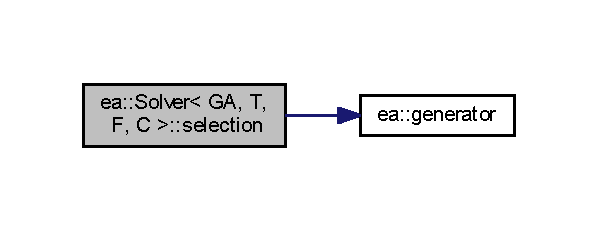
\includegraphics[width=287pt]{classea_1_1_solver_3_01_g_a_00_01_t_00_01_f_00_01_c_01_4_a1bc73c28211d7ba80665b286fbdea948_cgraph}
\end{center}
\end{figure}


\subsection{Friends And Related Function Documentation}
\mbox{\Hypertarget{classea_1_1_solver_3_01_g_a_00_01_t_00_01_f_00_01_c_01_4_a36e0662bcb575fd6a11cec4eedf85117}\label{classea_1_1_solver_3_01_g_a_00_01_t_00_01_f_00_01_c_01_4_a36e0662bcb575fd6a11cec4eedf85117}} 
\index{ea\+::\+Solver$<$ G\+A, T, F, C $>$@{ea\+::\+Solver$<$ G\+A, T, F, C $>$}!Solver\+\_\+base$<$ Solver$<$ G\+A, T, F, C $>$, G\+A, T, F, C $>$@{Solver\+\_\+base$<$ Solver$<$ G\+A, T, F, C $>$, G\+A, T, F, C $>$}}
\index{Solver\+\_\+base$<$ Solver$<$ G\+A, T, F, C $>$, G\+A, T, F, C $>$@{Solver\+\_\+base$<$ Solver$<$ G\+A, T, F, C $>$, G\+A, T, F, C $>$}!ea\+::\+Solver$<$ G\+A, T, F, C $>$@{ea\+::\+Solver$<$ G\+A, T, F, C $>$}}
\subsubsection{\texorpdfstring{Solver\+\_\+base$<$ Solver$<$ G\+A, T, F, C $>$, G\+A, T, F, C $>$}{Solver\_base< Solver< GA, T, F, C >, GA, T, F, C >}}
{\footnotesize\ttfamily template$<$typename T , typename F , typename C $>$ \\
friend class \hyperlink{classea_1_1_solver__base}{Solver\+\_\+base}$<$ \hyperlink{classea_1_1_solver}{Solver}$<$ \hyperlink{structea_1_1_g_a}{GA}, T, F, C $>$, \hyperlink{structea_1_1_g_a}{GA}, T, F, C $>$\hspace{0.3cm}{\ttfamily [friend]}}



Definition at line 76 of file geneticalgo.\+h.



\subsection{Member Data Documentation}
\mbox{\Hypertarget{classea_1_1_solver_3_01_g_a_00_01_t_00_01_f_00_01_c_01_4_a01dbd57c74c1ebd73e4ac976e29ecb33}\label{classea_1_1_solver_3_01_g_a_00_01_t_00_01_f_00_01_c_01_4_a01dbd57c74c1ebd73e4ac976e29ecb33}} 
\index{ea\+::\+Solver$<$ G\+A, T, F, C $>$@{ea\+::\+Solver$<$ G\+A, T, F, C $>$}!bdistribution@{bdistribution}}
\index{bdistribution@{bdistribution}!ea\+::\+Solver$<$ G\+A, T, F, C $>$@{ea\+::\+Solver$<$ G\+A, T, F, C $>$}}
\subsubsection{\texorpdfstring{bdistribution}{bdistribution}}
{\footnotesize\ttfamily template$<$typename T , typename F , typename C $>$ \\
boost\+::math\+::beta\+\_\+distribution$<$T$>$ \hyperlink{classea_1_1_solver}{ea\+::\+Solver}$<$ \hyperlink{structea_1_1_g_a}{GA}, T, F, C $>$\+::bdistribution\hspace{0.3cm}{\ttfamily [private]}}



Beta distribution. 



Definition at line 100 of file geneticalgo.\+h.

\mbox{\Hypertarget{classea_1_1_solver_3_01_g_a_00_01_t_00_01_f_00_01_c_01_4_a5e56c4d15894af96c2be5fcaec7d14fb}\label{classea_1_1_solver_3_01_g_a_00_01_t_00_01_f_00_01_c_01_4_a5e56c4d15894af96c2be5fcaec7d14fb}} 
\index{ea\+::\+Solver$<$ G\+A, T, F, C $>$@{ea\+::\+Solver$<$ G\+A, T, F, C $>$}!ga@{ga}}
\index{ga@{ga}!ea\+::\+Solver$<$ G\+A, T, F, C $>$@{ea\+::\+Solver$<$ G\+A, T, F, C $>$}}
\subsubsection{\texorpdfstring{ga}{ga}}
{\footnotesize\ttfamily template$<$typename T , typename F , typename C $>$ \\
const \hyperlink{structea_1_1_g_a}{GA}$<$T$>$\& \hyperlink{classea_1_1_solver}{ea\+::\+Solver}$<$ \hyperlink{structea_1_1_g_a}{GA}, T, F, C $>$\+::ga\hspace{0.3cm}{\ttfamily [private]}}



Genetic Algorithms structure used internally (reference to solver\+\_\+struct) 



Definition at line 94 of file geneticalgo.\+h.

\mbox{\Hypertarget{classea_1_1_solver_3_01_g_a_00_01_t_00_01_f_00_01_c_01_4_a805f49211363542de6984c7fd2c97c9c}\label{classea_1_1_solver_3_01_g_a_00_01_t_00_01_f_00_01_c_01_4_a805f49211363542de6984c7fd2c97c9c}} 
\index{ea\+::\+Solver$<$ G\+A, T, F, C $>$@{ea\+::\+Solver$<$ G\+A, T, F, C $>$}!npop@{npop}}
\index{npop@{npop}!ea\+::\+Solver$<$ G\+A, T, F, C $>$@{ea\+::\+Solver$<$ G\+A, T, F, C $>$}}
\subsubsection{\texorpdfstring{npop}{npop}}
{\footnotesize\ttfamily template$<$typename T , typename F , typename C $>$ \\
size\+\_\+t \hyperlink{classea_1_1_solver}{ea\+::\+Solver}$<$ \hyperlink{structea_1_1_g_a}{GA}, T, F, C $>$\+::npop\hspace{0.3cm}{\ttfamily [private]}}



Size of the population is mutable. 



Definition at line 96 of file geneticalgo.\+h.

\mbox{\Hypertarget{classea_1_1_solver_3_01_g_a_00_01_t_00_01_f_00_01_c_01_4_a097a7ec4bbcf9e5bade6e498d55d4d11}\label{classea_1_1_solver_3_01_g_a_00_01_t_00_01_f_00_01_c_01_4_a097a7ec4bbcf9e5bade6e498d55d4d11}} 
\index{ea\+::\+Solver$<$ G\+A, T, F, C $>$@{ea\+::\+Solver$<$ G\+A, T, F, C $>$}!stdev@{stdev}}
\index{stdev@{stdev}!ea\+::\+Solver$<$ G\+A, T, F, C $>$@{ea\+::\+Solver$<$ G\+A, T, F, C $>$}}
\subsubsection{\texorpdfstring{stdev}{stdev}}
{\footnotesize\ttfamily template$<$typename T , typename F , typename C $>$ \\
std\+::vector$<$T$>$ \hyperlink{classea_1_1_solver}{ea\+::\+Solver}$<$ \hyperlink{structea_1_1_g_a}{GA}, T, F, C $>$\+::stdev\hspace{0.3cm}{\ttfamily [private]}}



Standard deviation is mutable, so a copy is created. 



Definition at line 98 of file geneticalgo.\+h.



The documentation for this class was generated from the following file\+:\begin{DoxyCompactItemize}
\item 
\hyperlink{geneticalgo_8h}{geneticalgo.\+h}\end{DoxyCompactItemize}

\hypertarget{classea_1_1_solver_3_01_p_s_ol_00_01_t_00_01_f_00_01_c_01_4}{}\section{ea\+:\+:Solver$<$ P\+S\+Ol, T, F, C $>$ Class Template Reference}
\label{classea_1_1_solver_3_01_p_s_ol_00_01_t_00_01_f_00_01_c_01_4}\index{ea\+::\+Solver$<$ P\+S\+Ol, T, F, C $>$@{ea\+::\+Solver$<$ P\+S\+Ol, T, F, C $>$}}


Local Best Particle Swarm Optimisation (P\+SO) Class.  




{\ttfamily \#include $<$lbestpso.\+h$>$}



Inheritance diagram for ea\+:\+:Solver$<$ P\+S\+Ol, T, F, C $>$\+:
\nopagebreak
\begin{figure}[H]
\begin{center}
\leavevmode
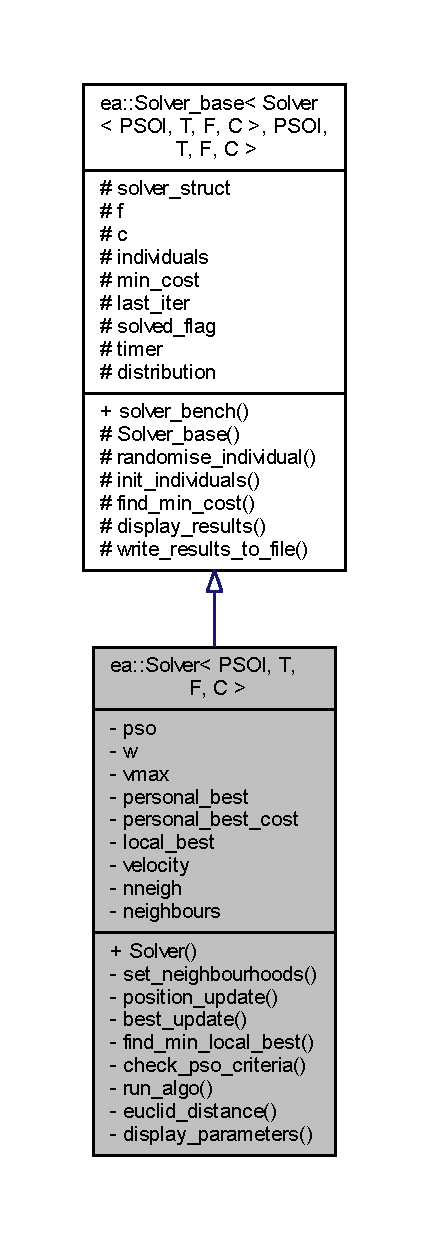
\includegraphics[height=550pt]{classea_1_1_solver_3_01_p_s_ol_00_01_t_00_01_f_00_01_c_01_4__inherit__graph}
\end{center}
\end{figure}
\subsection*{Public Member Functions}
\begin{DoxyCompactItemize}
\item 
\hyperlink{classea_1_1_solver_3_01_p_s_ol_00_01_t_00_01_f_00_01_c_01_4_aa27c4e1663fa5d0400cd75191e695f40}{Solver} (const \hyperlink{structea_1_1_p_s_ol}{P\+S\+Ol}$<$ T $>$ \&i\+\_\+pso, F \hyperlink{classea_1_1_solver__base_ae0a893780c93dfe17c1d17301de6494f}{f}, C \hyperlink{classea_1_1_solver__base_a6914e89d30e7484f2b4af1783f0de8c3}{c})
\begin{DoxyCompactList}\small\item\em Constructor. \end{DoxyCompactList}\end{DoxyCompactItemize}
\subsection*{Private Member Functions}
\begin{DoxyCompactItemize}
\item 
std\+::unordered\+\_\+map$<$ size\+\_\+t, std\+::array$<$ size\+\_\+t, 3 $>$ $>$ \hyperlink{classea_1_1_solver_3_01_p_s_ol_00_01_t_00_01_f_00_01_c_01_4_ae7599388d63b6905f4d9c49a3ad85387}{set\+\_\+neighbourhoods} ()
\begin{DoxyCompactList}\small\item\em Set the neighbourhoods of the algorithm using particle indices. \end{DoxyCompactList}\item 
void \hyperlink{classea_1_1_solver_3_01_p_s_ol_00_01_t_00_01_f_00_01_c_01_4_a9f20cae513cb6a44dddc59ef43ee206f}{position\+\_\+update} ()
\begin{DoxyCompactList}\small\item\em Position update of the particles. \end{DoxyCompactList}\item 
void \hyperlink{classea_1_1_solver_3_01_p_s_ol_00_01_t_00_01_f_00_01_c_01_4_a165112bf8f9e69d16c7a4d0680e1cd20}{best\+\_\+update} ()
\begin{DoxyCompactList}\small\item\em This method sets the personal and local best solutions. \end{DoxyCompactList}\item 
void \hyperlink{classea_1_1_solver_3_01_p_s_ol_00_01_t_00_01_f_00_01_c_01_4_ae7821ee945e33732ec24d47c88d4b310}{find\+\_\+min\+\_\+local\+\_\+best} ()
\begin{DoxyCompactList}\small\item\em This is a faster way to calculate the minimum cost unless there is only one neighbourhood, in which case it is the same as find\+\_\+min\+\_\+cost(\+F f) \end{DoxyCompactList}\item 
bool \hyperlink{classea_1_1_solver_3_01_p_s_ol_00_01_t_00_01_f_00_01_c_01_4_a474c18a8544f7ae0d5fe9d1587de2ad3}{check\+\_\+pso\+\_\+criteria} ()
\begin{DoxyCompactList}\small\item\em Define the maximum radius stopping criterion. \end{DoxyCompactList}\item 
void \hyperlink{classea_1_1_solver_3_01_p_s_ol_00_01_t_00_01_f_00_01_c_01_4_a0fa43e874bb60282a742c4c3dff651a9}{run\+\_\+algo} ()
\begin{DoxyCompactList}\small\item\em Runs the algorithm until stopping criteria return void. \end{DoxyCompactList}\item 
T \hyperlink{classea_1_1_solver_3_01_p_s_ol_00_01_t_00_01_f_00_01_c_01_4_a21df6a4efb4d058ecd3bc342e318b59a}{euclid\+\_\+distance} (const std\+::vector$<$ T $>$ \&x, const std\+::vector$<$ T $>$ \&y)
\begin{DoxyCompactList}\small\item\em Euclidean Distance of two vectors .. \end{DoxyCompactList}\item 
std\+::stringstream \hyperlink{classea_1_1_solver_3_01_p_s_ol_00_01_t_00_01_f_00_01_c_01_4_aaccd379111d0ebcf820fdce19ab23023}{display\+\_\+parameters} ()
\begin{DoxyCompactList}\small\item\em Display P\+SO parameters. \end{DoxyCompactList}\end{DoxyCompactItemize}
\subsection*{Private Attributes}
\begin{DoxyCompactItemize}
\item 
const \hyperlink{structea_1_1_p_s_ol}{P\+S\+Ol}$<$ T $>$ \& \hyperlink{classea_1_1_solver_3_01_p_s_ol_00_01_t_00_01_f_00_01_c_01_4_a3098f083ef04a0ce7ae0eef22dd80442}{pso}
\begin{DoxyCompactList}\small\item\em Particle Swarm Optimisation structure used internally (reference to solver\+\_\+struct) \end{DoxyCompactList}\item 
T \hyperlink{classea_1_1_solver_3_01_p_s_ol_00_01_t_00_01_f_00_01_c_01_4_a5c9d1a207892da92e2cf689b24c256ee}{w}
\begin{DoxyCompactList}\small\item\em Inertia is mutable, so a copy is created. \end{DoxyCompactList}\item 
std\+::vector$<$ T $>$ \hyperlink{classea_1_1_solver_3_01_p_s_ol_00_01_t_00_01_f_00_01_c_01_4_abd93da2229dac4eb2d11f4904a65ae9a}{vmax}
\begin{DoxyCompactList}\small\item\em Maximum Velocity is mutable, so a copy is created. \end{DoxyCompactList}\item 
std\+::vector$<$ std\+::vector$<$ T $>$ $>$ \hyperlink{classea_1_1_solver_3_01_p_s_ol_00_01_t_00_01_f_00_01_c_01_4_a0738e0ab079273c4d34c827fad533868}{personal\+\_\+best}
\begin{DoxyCompactList}\small\item\em Personal best vector of the particles, holds the best position recorded for each particle. \end{DoxyCompactList}\item 
std\+::vector$<$ T $>$ \hyperlink{classea_1_1_solver_3_01_p_s_ol_00_01_t_00_01_f_00_01_c_01_4_ae728d584641709062919b0cedd3e77cc}{personal\+\_\+best\+\_\+cost}
\begin{DoxyCompactList}\small\item\em Personal best cost vector of the particles. \end{DoxyCompactList}\item 
std\+::vector$<$ std\+::vector$<$ T $>$ $>$ \hyperlink{classea_1_1_solver_3_01_p_s_ol_00_01_t_00_01_f_00_01_c_01_4_a6671c3d551564e3b4cd0944bfb2c33fd}{local\+\_\+best}
\begin{DoxyCompactList}\small\item\em Local best vector, holds the best position recorded for each neighbourhood. \end{DoxyCompactList}\item 
std\+::vector$<$ std\+::vector$<$ T $>$ $>$ \hyperlink{classea_1_1_solver_3_01_p_s_ol_00_01_t_00_01_f_00_01_c_01_4_ae8293610cb6bffc00e0fda749754a1f2}{velocity}
\begin{DoxyCompactList}\small\item\em Velocity of the particles. \end{DoxyCompactList}\item 
const size\+\_\+t \hyperlink{classea_1_1_solver_3_01_p_s_ol_00_01_t_00_01_f_00_01_c_01_4_adb34cfcd87307ee2271b5aa5ffdd779d}{nneigh}
\begin{DoxyCompactList}\small\item\em Number of neighbourhoods. \end{DoxyCompactList}\item 
std\+::unordered\+\_\+map$<$ size\+\_\+t, std\+::array$<$ size\+\_\+t, 3 $>$ $>$ \hyperlink{classea_1_1_solver_3_01_p_s_ol_00_01_t_00_01_f_00_01_c_01_4_ab92e8a0460092b8264bd9023a3455257}{neighbours}
\begin{DoxyCompactList}\small\item\em Neighbours of each particle. \end{DoxyCompactList}\end{DoxyCompactItemize}
\subsection*{Friends}
\begin{DoxyCompactItemize}
\item 
class \hyperlink{classea_1_1_solver_3_01_p_s_ol_00_01_t_00_01_f_00_01_c_01_4_a95bfc162c6509fec9ecb02185ed094d3}{Solver\+\_\+base$<$ Solver$<$ P\+S\+Ol, T, F, C $>$, P\+S\+Ol, T, F, C $>$}
\end{DoxyCompactItemize}
\subsection*{Additional Inherited Members}


\subsection{Detailed Description}
\subsubsection*{template$<$typename T, typename F, typename C$>$\newline
class ea\+::\+Solver$<$ P\+S\+Ol, T, F, C $>$}

Local Best Particle Swarm Optimisation (P\+SO) Class. 

Definition at line 69 of file lbestpso.\+h.



\subsection{Constructor \& Destructor Documentation}
\mbox{\Hypertarget{classea_1_1_solver_3_01_p_s_ol_00_01_t_00_01_f_00_01_c_01_4_aa27c4e1663fa5d0400cd75191e695f40}\label{classea_1_1_solver_3_01_p_s_ol_00_01_t_00_01_f_00_01_c_01_4_aa27c4e1663fa5d0400cd75191e695f40}} 
\index{ea\+::\+Solver$<$ P\+S\+Ol, T, F, C $>$@{ea\+::\+Solver$<$ P\+S\+Ol, T, F, C $>$}!Solver@{Solver}}
\index{Solver@{Solver}!ea\+::\+Solver$<$ P\+S\+Ol, T, F, C $>$@{ea\+::\+Solver$<$ P\+S\+Ol, T, F, C $>$}}
\subsubsection{\texorpdfstring{Solver()}{Solver()}}
{\footnotesize\ttfamily template$<$typename T , typename F , typename C $>$ \\
\hyperlink{classea_1_1_solver}{ea\+::\+Solver}$<$ \hyperlink{structea_1_1_p_s_ol}{P\+S\+Ol}, T, F, C $>$\+::\hyperlink{classea_1_1_solver}{Solver} (\begin{DoxyParamCaption}\item[{const \hyperlink{structea_1_1_p_s_ol}{P\+S\+Ol}$<$ T $>$ \&}]{i\+\_\+pso,  }\item[{F}]{f,  }\item[{C}]{c }\end{DoxyParamCaption})\hspace{0.3cm}{\ttfamily [inline]}}



Constructor. 


\begin{DoxyParams}{Parameters}
{\em i\+\_\+pso} & The particle swarm optimisation parameter structure that is used to construct the solver \\
\hline
{\em f} & A reference to the objective function \\
\hline
{\em c} & A reference to the constraints function \\
\hline
\end{DoxyParams}
\begin{DoxyReturn}{Returns}
A Solver$<$\+P\+S\+O, T, F, C$>$ object 
\end{DoxyReturn}


Definition at line 80 of file lbestpso.\+h.


\begin{DoxyCode}
80                                                :
81             Solver\_base<Solver<PSOl, T, F, C>, PSOl, T, F, C>(i\_pso, \hyperlink{classea_1_1_solver__base_ae0a893780c93dfe17c1d17301de6494f}{f}, \hyperlink{classea_1_1_solver__base_a6914e89d30e7484f2b4af1783f0de8c3}{c}),
82             \hyperlink{classea_1_1_solver_3_01_p_s_ol_00_01_t_00_01_f_00_01_c_01_4_a3098f083ef04a0ce7ae0eef22dd80442}{pso}(this->\hyperlink{classea_1_1_solver__base_a5e1d821809f2d26c6f882942ad728127}{solver\_struct}),
83             \hyperlink{classea_1_1_solver_3_01_p_s_ol_00_01_t_00_01_f_00_01_c_01_4_a5c9d1a207892da92e2cf689b24c256ee}{w}(i\_pso.w),
84             \hyperlink{classea_1_1_solver_3_01_p_s_ol_00_01_t_00_01_f_00_01_c_01_4_abd93da2229dac4eb2d11f4904a65ae9a}{vmax}(i\_pso.vmax),
85             \hyperlink{classea_1_1_solver_3_01_p_s_ol_00_01_t_00_01_f_00_01_c_01_4_adb34cfcd87307ee2271b5aa5ffdd779d}{nneigh}(i\_pso.npop),
86             \hyperlink{classea_1_1_solver_3_01_p_s_ol_00_01_t_00_01_f_00_01_c_01_4_ab92e8a0460092b8264bd9023a3455257}{neighbours}(\hyperlink{classea_1_1_solver_3_01_p_s_ol_00_01_t_00_01_f_00_01_c_01_4_ae7599388d63b6905f4d9c49a3ad85387}{set\_neighbourhoods}())
87         \{
88             \hyperlink{classea_1_1_solver_3_01_p_s_ol_00_01_t_00_01_f_00_01_c_01_4_ae8293610cb6bffc00e0fda749754a1f2}{velocity}.resize(\hyperlink{classea_1_1_solver_3_01_p_s_ol_00_01_t_00_01_f_00_01_c_01_4_a3098f083ef04a0ce7ae0eef22dd80442}{pso}.npop, std::vector<T>(\hyperlink{classea_1_1_solver_3_01_p_s_ol_00_01_t_00_01_f_00_01_c_01_4_a3098f083ef04a0ce7ae0eef22dd80442}{pso}.ndv));
89             \hyperlink{classea_1_1_solver_3_01_p_s_ol_00_01_t_00_01_f_00_01_c_01_4_a6671c3d551564e3b4cd0944bfb2c33fd}{local\_best}.resize(\hyperlink{classea_1_1_solver_3_01_p_s_ol_00_01_t_00_01_f_00_01_c_01_4_adb34cfcd87307ee2271b5aa5ffdd779d}{nneigh});
90             \textcolor{keywordflow}{for} (\textcolor{keyword}{auto}& p : \hyperlink{classea_1_1_solver_3_01_p_s_ol_00_01_t_00_01_f_00_01_c_01_4_ae8293610cb6bffc00e0fda749754a1f2}{velocity})
91             \{
92                 \textcolor{keywordflow}{for} (\textcolor{keyword}{auto}& n : p)
93                 \{
94                     n = 0.0;
95                 \}
96             \}
97             \textcolor{keywordflow}{for} (\textcolor{keyword}{const} \textcolor{keyword}{auto}& p : this->\hyperlink{classea_1_1_solver__base_ad75bc440d24a46e97694c7c889f2ecde}{individuals})
98             \{
99                 \hyperlink{classea_1_1_solver_3_01_p_s_ol_00_01_t_00_01_f_00_01_c_01_4_a0738e0ab079273c4d34c827fad533868}{personal\_best}.push\_back(p);
100                 \hyperlink{classea_1_1_solver_3_01_p_s_ol_00_01_t_00_01_f_00_01_c_01_4_ae728d584641709062919b0cedd3e77cc}{personal\_best\_cost}.push\_back(\hyperlink{classea_1_1_solver__base_ae0a893780c93dfe17c1d17301de6494f}{f}(p));
101             \}
102             \textcolor{keywordflow}{for} (\textcolor{keyword}{auto}& p : \hyperlink{classea_1_1_solver_3_01_p_s_ol_00_01_t_00_01_f_00_01_c_01_4_a6671c3d551564e3b4cd0944bfb2c33fd}{local\_best})
103             \{
104                 p = \hyperlink{classea_1_1_solver_3_01_p_s_ol_00_01_t_00_01_f_00_01_c_01_4_a0738e0ab079273c4d34c827fad533868}{personal\_best}[0];
105             \}
106             \textcolor{keywordflow}{for} (\textcolor{keywordtype}{size\_t} i = 0; i < \hyperlink{classea_1_1_solver_3_01_p_s_ol_00_01_t_00_01_f_00_01_c_01_4_a3098f083ef04a0ce7ae0eef22dd80442}{pso}.npop; ++i)
107             \{
108                 \textcolor{keywordflow}{for} (\textcolor{keyword}{const} \textcolor{keyword}{auto}& index : \hyperlink{classea_1_1_solver_3_01_p_s_ol_00_01_t_00_01_f_00_01_c_01_4_ab92e8a0460092b8264bd9023a3455257}{neighbours}[i])
109                 \{
110                     \textcolor{keywordflow}{if} (\hyperlink{classea_1_1_solver_3_01_p_s_ol_00_01_t_00_01_f_00_01_c_01_4_ae728d584641709062919b0cedd3e77cc}{personal\_best\_cost}[index] < this->\hyperlink{classea_1_1_solver__base_ae0a893780c93dfe17c1d17301de6494f}{f}(local\_best[i]))
111                     \{
112                         local\_best[i] = \hyperlink{classea_1_1_solver_3_01_p_s_ol_00_01_t_00_01_f_00_01_c_01_4_a0738e0ab079273c4d34c827fad533868}{personal\_best}[index];
113                     \}
114                 \}
115             \}
116             \hyperlink{classea_1_1_solver_3_01_p_s_ol_00_01_t_00_01_f_00_01_c_01_4_ae7821ee945e33732ec24d47c88d4b310}{find\_min\_local\_best}();
117         \}
\end{DoxyCode}


\subsection{Member Function Documentation}
\mbox{\Hypertarget{classea_1_1_solver_3_01_p_s_ol_00_01_t_00_01_f_00_01_c_01_4_a165112bf8f9e69d16c7a4d0680e1cd20}\label{classea_1_1_solver_3_01_p_s_ol_00_01_t_00_01_f_00_01_c_01_4_a165112bf8f9e69d16c7a4d0680e1cd20}} 
\index{ea\+::\+Solver$<$ P\+S\+Ol, T, F, C $>$@{ea\+::\+Solver$<$ P\+S\+Ol, T, F, C $>$}!best\+\_\+update@{best\+\_\+update}}
\index{best\+\_\+update@{best\+\_\+update}!ea\+::\+Solver$<$ P\+S\+Ol, T, F, C $>$@{ea\+::\+Solver$<$ P\+S\+Ol, T, F, C $>$}}
\subsubsection{\texorpdfstring{best\+\_\+update()}{best\_update()}}
{\footnotesize\ttfamily template$<$typename T , typename F , typename C $>$ \\
void \hyperlink{classea_1_1_solver}{ea\+::\+Solver}$<$ \hyperlink{structea_1_1_p_s_ol}{P\+S\+Ol}, T, F, C $>$\+::best\+\_\+update (\begin{DoxyParamCaption}{ }\end{DoxyParamCaption})\hspace{0.3cm}{\ttfamily [private]}}



This method sets the personal and local best solutions. 

\begin{DoxyReturn}{Returns}
void 
\end{DoxyReturn}


Definition at line 257 of file lbestpso.\+h.


\begin{DoxyCode}
258     \{
259         \textcolor{keywordflow}{for} (\textcolor{keywordtype}{size\_t} i = 0; i < \hyperlink{classea_1_1_solver_3_01_p_s_ol_00_01_t_00_01_f_00_01_c_01_4_a3098f083ef04a0ce7ae0eef22dd80442}{pso}.npop; ++i)
260         \{
261         \}
262     \}
\end{DoxyCode}
\mbox{\Hypertarget{classea_1_1_solver_3_01_p_s_ol_00_01_t_00_01_f_00_01_c_01_4_a474c18a8544f7ae0d5fe9d1587de2ad3}\label{classea_1_1_solver_3_01_p_s_ol_00_01_t_00_01_f_00_01_c_01_4_a474c18a8544f7ae0d5fe9d1587de2ad3}} 
\index{ea\+::\+Solver$<$ P\+S\+Ol, T, F, C $>$@{ea\+::\+Solver$<$ P\+S\+Ol, T, F, C $>$}!check\+\_\+pso\+\_\+criteria@{check\+\_\+pso\+\_\+criteria}}
\index{check\+\_\+pso\+\_\+criteria@{check\+\_\+pso\+\_\+criteria}!ea\+::\+Solver$<$ P\+S\+Ol, T, F, C $>$@{ea\+::\+Solver$<$ P\+S\+Ol, T, F, C $>$}}
\subsubsection{\texorpdfstring{check\+\_\+pso\+\_\+criteria()}{check\_pso\_criteria()}}
{\footnotesize\ttfamily template$<$typename T , typename F , typename C $>$ \\
bool \hyperlink{classea_1_1_solver}{ea\+::\+Solver}$<$ \hyperlink{structea_1_1_p_s_ol}{P\+S\+Ol}, T, F, C $>$\+::check\+\_\+pso\+\_\+criteria (\begin{DoxyParamCaption}{ }\end{DoxyParamCaption})\hspace{0.3cm}{\ttfamily [private]}}



Define the maximum radius stopping criterion. 

\begin{DoxyReturn}{Returns}
true if criteria are met, false otherwise 
\end{DoxyReturn}


Definition at line 277 of file lbestpso.\+h.


\begin{DoxyCode}
278     \{
279         std::vector<T> distance(\hyperlink{classea_1_1_solver_3_01_p_s_ol_00_01_t_00_01_f_00_01_c_01_4_a3098f083ef04a0ce7ae0eef22dd80442}{pso}.npop);
280         \textcolor{keywordflow}{for} (\textcolor{keywordtype}{size\_t} i = 0; i < \hyperlink{classea_1_1_solver_3_01_p_s_ol_00_01_t_00_01_f_00_01_c_01_4_a3098f083ef04a0ce7ae0eef22dd80442}{pso}.npop; ++i)
281         \{
282             distance[i] = \hyperlink{classea_1_1_solver_3_01_p_s_ol_00_01_t_00_01_f_00_01_c_01_4_a21df6a4efb4d058ecd3bc342e318b59a}{euclid\_distance}(this->\hyperlink{classea_1_1_solver__base_ad75bc440d24a46e97694c7c889f2ecde}{individuals}[i], this->
      \hyperlink{classea_1_1_solver__base_af745cded954be26280d842c1e7c7f989}{min\_cost});
283         \}
284         T rmax = distance[0];
285         \textcolor{keywordflow}{for} (\textcolor{keywordtype}{size\_t} i = 0; i < \hyperlink{classea_1_1_solver_3_01_p_s_ol_00_01_t_00_01_f_00_01_c_01_4_a3098f083ef04a0ce7ae0eef22dd80442}{pso}.npop; ++i)
286         \{
287             \textcolor{keywordflow}{if} (rmax < distance[i])
288             \{
289                 rmax = distance[i];
290             \}
291             \textcolor{keywordflow}{else}
292             \{
293             \}
294         \}
295         \textcolor{keywordflow}{if} (\hyperlink{classea_1_1_solver_3_01_p_s_ol_00_01_t_00_01_f_00_01_c_01_4_a3098f083ef04a0ce7ae0eef22dd80442}{pso}.tol > std::abs(this->f(this->min\_cost)))\textcolor{comment}{// || rmax < pso.tol)}
296         \{
297             \textcolor{keywordflow}{return} \textcolor{keyword}{true};
298         \}
299         \textcolor{keywordflow}{else}
300         \{
301             \textcolor{keywordflow}{return} \textcolor{keyword}{false};
302         \}
303     \}
\end{DoxyCode}
\mbox{\Hypertarget{classea_1_1_solver_3_01_p_s_ol_00_01_t_00_01_f_00_01_c_01_4_aaccd379111d0ebcf820fdce19ab23023}\label{classea_1_1_solver_3_01_p_s_ol_00_01_t_00_01_f_00_01_c_01_4_aaccd379111d0ebcf820fdce19ab23023}} 
\index{ea\+::\+Solver$<$ P\+S\+Ol, T, F, C $>$@{ea\+::\+Solver$<$ P\+S\+Ol, T, F, C $>$}!display\+\_\+parameters@{display\+\_\+parameters}}
\index{display\+\_\+parameters@{display\+\_\+parameters}!ea\+::\+Solver$<$ P\+S\+Ol, T, F, C $>$@{ea\+::\+Solver$<$ P\+S\+Ol, T, F, C $>$}}
\subsubsection{\texorpdfstring{display\+\_\+parameters()}{display\_parameters()}}
{\footnotesize\ttfamily template$<$typename T , typename F , typename C $>$ \\
\hyperlink{classea_1_1_solver}{ea\+::\+Solver}$<$ \hyperlink{structea_1_1_p_s_ol}{P\+S\+Ol}, T, F, C $>$\+::display\+\_\+parameters (\begin{DoxyParamCaption}{ }\end{DoxyParamCaption})\hspace{0.3cm}{\ttfamily [inline]}, {\ttfamily [private]}}



Display P\+SO parameters. 

\begin{DoxyReturn}{Returns}
A std\+::stringstream of the parameters 
\end{DoxyReturn}


Definition at line 185 of file lbestpso.\+h.



References ea\+::\+P\+S\+Ol$<$ T $>$\+::c, ea\+::\+P\+S\+Ol$<$ T $>$\+::vmax, and ea\+::\+P\+S\+Ol$<$ T $>$\+::w.


\begin{DoxyCode}
186         \{
187             std::stringstream parameters;
188             parameters << \textcolor{stringliteral}{"C:"} << \textcolor{stringliteral}{","} << \hyperlink{classea_1_1_solver_3_01_p_s_ol_00_01_t_00_01_f_00_01_c_01_4_a3098f083ef04a0ce7ae0eef22dd80442}{pso}.c << \textcolor{stringliteral}{","};
189             parameters << \textcolor{stringliteral}{"Inertia:"} << \textcolor{stringliteral}{","} << \hyperlink{classea_1_1_solver_3_01_p_s_ol_00_01_t_00_01_f_00_01_c_01_4_a3098f083ef04a0ce7ae0eef22dd80442}{pso}.w << \textcolor{stringliteral}{","};
190             parameters << \textcolor{stringliteral}{"Maximum Velocity:"} << \textcolor{stringliteral}{","} << \hyperlink{classea_1_1_solver_3_01_p_s_ol_00_01_t_00_01_f_00_01_c_01_4_a3098f083ef04a0ce7ae0eef22dd80442}{pso}.vmax;
191             \textcolor{keywordflow}{return} parameters;
192         \}
\end{DoxyCode}
\mbox{\Hypertarget{classea_1_1_solver_3_01_p_s_ol_00_01_t_00_01_f_00_01_c_01_4_a21df6a4efb4d058ecd3bc342e318b59a}\label{classea_1_1_solver_3_01_p_s_ol_00_01_t_00_01_f_00_01_c_01_4_a21df6a4efb4d058ecd3bc342e318b59a}} 
\index{ea\+::\+Solver$<$ P\+S\+Ol, T, F, C $>$@{ea\+::\+Solver$<$ P\+S\+Ol, T, F, C $>$}!euclid\+\_\+distance@{euclid\+\_\+distance}}
\index{euclid\+\_\+distance@{euclid\+\_\+distance}!ea\+::\+Solver$<$ P\+S\+Ol, T, F, C $>$@{ea\+::\+Solver$<$ P\+S\+Ol, T, F, C $>$}}
\subsubsection{\texorpdfstring{euclid\+\_\+distance()}{euclid\_distance()}}
{\footnotesize\ttfamily template$<$typename T , typename F , typename C $>$ \\
\hyperlink{classea_1_1_solver}{ea\+::\+Solver}$<$ \hyperlink{structea_1_1_p_s_ol}{P\+S\+Ol}, T, F, C $>$\+::euclid\+\_\+distance (\begin{DoxyParamCaption}\item[{const std\+::vector$<$ T $>$ \&}]{x,  }\item[{const std\+::vector$<$ T $>$ \&}]{y }\end{DoxyParamCaption})\hspace{0.3cm}{\ttfamily [inline]}, {\ttfamily [private]}}



Euclidean Distance of two vectors .. 


\begin{DoxyParams}{Parameters}
{\em x,y} & The two vectors for which the distance is calculated \\
\hline
\end{DoxyParams}
\begin{DoxyReturn}{Returns}
Distance as a floating-\/point number 
\end{DoxyReturn}


Definition at line 172 of file lbestpso.\+h.


\begin{DoxyCode}
173         \{
174             T sum = 0;
175             \textcolor{keywordflow}{for} (\textcolor{keywordtype}{size\_t} i = 0; i < x.size(); ++i)
176             \{
177                 sum = sum + std::pow(x[i] - y[i], 2);
178             \}
179             \textcolor{keywordflow}{return} std::sqrt(sum);
180         \}
\end{DoxyCode}
\mbox{\Hypertarget{classea_1_1_solver_3_01_p_s_ol_00_01_t_00_01_f_00_01_c_01_4_ae7821ee945e33732ec24d47c88d4b310}\label{classea_1_1_solver_3_01_p_s_ol_00_01_t_00_01_f_00_01_c_01_4_ae7821ee945e33732ec24d47c88d4b310}} 
\index{ea\+::\+Solver$<$ P\+S\+Ol, T, F, C $>$@{ea\+::\+Solver$<$ P\+S\+Ol, T, F, C $>$}!find\+\_\+min\+\_\+local\+\_\+best@{find\+\_\+min\+\_\+local\+\_\+best}}
\index{find\+\_\+min\+\_\+local\+\_\+best@{find\+\_\+min\+\_\+local\+\_\+best}!ea\+::\+Solver$<$ P\+S\+Ol, T, F, C $>$@{ea\+::\+Solver$<$ P\+S\+Ol, T, F, C $>$}}
\subsubsection{\texorpdfstring{find\+\_\+min\+\_\+local\+\_\+best()}{find\_min\_local\_best()}}
{\footnotesize\ttfamily template$<$typename T , typename F , typename C $>$ \\
void \hyperlink{classea_1_1_solver}{ea\+::\+Solver}$<$ \hyperlink{structea_1_1_p_s_ol}{P\+S\+Ol}, T, F, C $>$\+::find\+\_\+min\+\_\+local\+\_\+best (\begin{DoxyParamCaption}{ }\end{DoxyParamCaption})\hspace{0.3cm}{\ttfamily [private]}}



This is a faster way to calculate the minimum cost unless there is only one neighbourhood, in which case it is the same as find\+\_\+min\+\_\+cost(\+F f) 

\begin{DoxyReturn}{Returns}
void 
\end{DoxyReturn}


Definition at line 265 of file lbestpso.\+h.


\begin{DoxyCode}
266     \{
267         \textcolor{keywordflow}{for} (\textcolor{keywordtype}{size\_t} k = 0; k < \hyperlink{classea_1_1_solver_3_01_p_s_ol_00_01_t_00_01_f_00_01_c_01_4_adb34cfcd87307ee2271b5aa5ffdd779d}{nneigh}; ++k)
268         \{
269             \textcolor{keywordflow}{if} (this->\hyperlink{classea_1_1_solver__base_ae0a893780c93dfe17c1d17301de6494f}{f}(\hyperlink{classea_1_1_solver_3_01_p_s_ol_00_01_t_00_01_f_00_01_c_01_4_a6671c3d551564e3b4cd0944bfb2c33fd}{local\_best}[k]) < this->\hyperlink{classea_1_1_solver__base_ae0a893780c93dfe17c1d17301de6494f}{f}(this->\hyperlink{classea_1_1_solver__base_af745cded954be26280d842c1e7c7f989}{min\_cost}))
270             \{
271                 this->\hyperlink{classea_1_1_solver__base_af745cded954be26280d842c1e7c7f989}{min\_cost} = \hyperlink{classea_1_1_solver_3_01_p_s_ol_00_01_t_00_01_f_00_01_c_01_4_a6671c3d551564e3b4cd0944bfb2c33fd}{local\_best}[k];
272             \}
273         \}
274     \}
\end{DoxyCode}
\mbox{\Hypertarget{classea_1_1_solver_3_01_p_s_ol_00_01_t_00_01_f_00_01_c_01_4_a9f20cae513cb6a44dddc59ef43ee206f}\label{classea_1_1_solver_3_01_p_s_ol_00_01_t_00_01_f_00_01_c_01_4_a9f20cae513cb6a44dddc59ef43ee206f}} 
\index{ea\+::\+Solver$<$ P\+S\+Ol, T, F, C $>$@{ea\+::\+Solver$<$ P\+S\+Ol, T, F, C $>$}!position\+\_\+update@{position\+\_\+update}}
\index{position\+\_\+update@{position\+\_\+update}!ea\+::\+Solver$<$ P\+S\+Ol, T, F, C $>$@{ea\+::\+Solver$<$ P\+S\+Ol, T, F, C $>$}}
\subsubsection{\texorpdfstring{position\+\_\+update()}{position\_update()}}
{\footnotesize\ttfamily template$<$typename T , typename F , typename C $>$ \\
void \hyperlink{classea_1_1_solver}{ea\+::\+Solver}$<$ \hyperlink{structea_1_1_p_s_ol}{P\+S\+Ol}, T, F, C $>$\+::position\+\_\+update (\begin{DoxyParamCaption}{ }\end{DoxyParamCaption})\hspace{0.3cm}{\ttfamily [private]}}



Position update of the particles. 

\begin{DoxyReturn}{Returns}
void 
\end{DoxyReturn}
Checks that the candidate is feasible 

Definition at line 221 of file lbestpso.\+h.



References ea\+::\+P\+S\+Ol$<$ T $>$\+::c, ea\+::generator(), ea\+::\+P\+S\+Ol$<$ T $>$\+::vmax, and ea\+::\+P\+S\+Ol$<$ T $>$\+::w.


\begin{DoxyCode}
222     \{
223         \textcolor{keywordflow}{for} (\textcolor{keywordtype}{size\_t} i = 0; i < \hyperlink{classea_1_1_solver_3_01_p_s_ol_00_01_t_00_01_f_00_01_c_01_4_a3098f083ef04a0ce7ae0eef22dd80442}{pso}.npop; ++i)
224         \{
225             \textcolor{keywordflow}{for} (\textcolor{keywordtype}{size\_t} j = 0; j < \hyperlink{classea_1_1_solver_3_01_p_s_ol_00_01_t_00_01_f_00_01_c_01_4_a3098f083ef04a0ce7ae0eef22dd80442}{pso}.ndv; ++j)
226             \{
227                 std::uniform\_real\_distribution<double> \hyperlink{classea_1_1_solver__base_a6914e89d30e7484f2b4af1783f0de8c3}{c}(0, \hyperlink{classea_1_1_solver_3_01_p_s_ol_00_01_t_00_01_f_00_01_c_01_4_a3098f083ef04a0ce7ae0eef22dd80442}{pso}.c);
228                 \hyperlink{classea_1_1_solver_3_01_p_s_ol_00_01_t_00_01_f_00_01_c_01_4_ae8293610cb6bffc00e0fda749754a1f2}{velocity}[i][j] = \hyperlink{classea_1_1_solver_3_01_p_s_ol_00_01_t_00_01_f_00_01_c_01_4_a5c9d1a207892da92e2cf689b24c256ee}{w} * \hyperlink{classea_1_1_solver_3_01_p_s_ol_00_01_t_00_01_f_00_01_c_01_4_ae8293610cb6bffc00e0fda749754a1f2}{velocity}[i][j] + \hyperlink{classea_1_1_solver__base_a6914e89d30e7484f2b4af1783f0de8c3}{c}(
      \hyperlink{namespaceea_a385e8ca8ba4ae2f69dcfffa79f20c2ff}{generator}) * (\hyperlink{classea_1_1_solver_3_01_p_s_ol_00_01_t_00_01_f_00_01_c_01_4_a0738e0ab079273c4d34c827fad533868}{personal\_best}[i][j] - this->\hyperlink{classea_1_1_solver__base_ad75bc440d24a46e97694c7c889f2ecde}{individuals}[i][j])
229                     + \hyperlink{classea_1_1_solver__base_a6914e89d30e7484f2b4af1783f0de8c3}{c}(\hyperlink{namespaceea_a385e8ca8ba4ae2f69dcfffa79f20c2ff}{generator}) * (\hyperlink{classea_1_1_solver_3_01_p_s_ol_00_01_t_00_01_f_00_01_c_01_4_a6671c3d551564e3b4cd0944bfb2c33fd}{local\_best}[i][j] - this->
      \hyperlink{classea_1_1_solver__base_ad75bc440d24a46e97694c7c889f2ecde}{individuals}[i][j]);
230                 \textcolor{keywordflow}{if} (\hyperlink{classea_1_1_solver_3_01_p_s_ol_00_01_t_00_01_f_00_01_c_01_4_ae8293610cb6bffc00e0fda749754a1f2}{velocity}[i][j] > \hyperlink{classea_1_1_solver_3_01_p_s_ol_00_01_t_00_01_f_00_01_c_01_4_abd93da2229dac4eb2d11f4904a65ae9a}{vmax}[j])
231                 \{
232                     \hyperlink{classea_1_1_solver_3_01_p_s_ol_00_01_t_00_01_f_00_01_c_01_4_ae8293610cb6bffc00e0fda749754a1f2}{velocity}[i][j] = \hyperlink{classea_1_1_solver_3_01_p_s_ol_00_01_t_00_01_f_00_01_c_01_4_abd93da2229dac4eb2d11f4904a65ae9a}{vmax}[j];
233                 \}
234                 this->\hyperlink{classea_1_1_solver__base_ad75bc440d24a46e97694c7c889f2ecde}{individuals}[i][j] = this->\hyperlink{classea_1_1_solver__base_ad75bc440d24a46e97694c7c889f2ecde}{individuals}[i][j] + 
      \hyperlink{classea_1_1_solver_3_01_p_s_ol_00_01_t_00_01_f_00_01_c_01_4_ae8293610cb6bffc00e0fda749754a1f2}{velocity}[i][j];
235             \}
237             \textcolor{keywordflow}{if} (!this->\hyperlink{classea_1_1_solver__base_a6914e89d30e7484f2b4af1783f0de8c3}{c}(this->\hyperlink{classea_1_1_solver__base_ad75bc440d24a46e97694c7c889f2ecde}{individuals}[i]))
238             \{
239                 this->\hyperlink{classea_1_1_solver__base_ad75bc440d24a46e97694c7c889f2ecde}{individuals}[i] = \hyperlink{classea_1_1_solver_3_01_p_s_ol_00_01_t_00_01_f_00_01_c_01_4_a0738e0ab079273c4d34c827fad533868}{personal\_best}[i];
240             \}
241             \textcolor{keywordflow}{if} (this->\hyperlink{classea_1_1_solver__base_ae0a893780c93dfe17c1d17301de6494f}{f}(this->\hyperlink{classea_1_1_solver__base_ad75bc440d24a46e97694c7c889f2ecde}{individuals}[i]) < this->\hyperlink{classea_1_1_solver__base_ae0a893780c93dfe17c1d17301de6494f}{f}(
      \hyperlink{classea_1_1_solver_3_01_p_s_ol_00_01_t_00_01_f_00_01_c_01_4_a0738e0ab079273c4d34c827fad533868}{personal\_best}[i]))
242             \{
243                 \hyperlink{classea_1_1_solver_3_01_p_s_ol_00_01_t_00_01_f_00_01_c_01_4_a0738e0ab079273c4d34c827fad533868}{personal\_best}[i] = this->\hyperlink{classea_1_1_solver__base_ad75bc440d24a46e97694c7c889f2ecde}{individuals}[i];
244                 \hyperlink{classea_1_1_solver_3_01_p_s_ol_00_01_t_00_01_f_00_01_c_01_4_ae728d584641709062919b0cedd3e77cc}{personal\_best\_cost}[i] = this->\hyperlink{classea_1_1_solver__base_ae0a893780c93dfe17c1d17301de6494f}{f}(this->
      \hyperlink{classea_1_1_solver__base_ad75bc440d24a46e97694c7c889f2ecde}{individuals}[i]);
245             \}
246             \textcolor{keywordflow}{for} (\textcolor{keyword}{const} \textcolor{keyword}{auto}& index : \hyperlink{classea_1_1_solver_3_01_p_s_ol_00_01_t_00_01_f_00_01_c_01_4_ab92e8a0460092b8264bd9023a3455257}{neighbours}[i])
247             \{
248                 \textcolor{keywordflow}{if} (\hyperlink{classea_1_1_solver_3_01_p_s_ol_00_01_t_00_01_f_00_01_c_01_4_ae728d584641709062919b0cedd3e77cc}{personal\_best\_cost}[index] < this->\hyperlink{classea_1_1_solver__base_ae0a893780c93dfe17c1d17301de6494f}{f}(
      \hyperlink{classea_1_1_solver_3_01_p_s_ol_00_01_t_00_01_f_00_01_c_01_4_a6671c3d551564e3b4cd0944bfb2c33fd}{local\_best}[i]))
249                 \{
250                     \hyperlink{classea_1_1_solver_3_01_p_s_ol_00_01_t_00_01_f_00_01_c_01_4_a6671c3d551564e3b4cd0944bfb2c33fd}{local\_best}[i] = \hyperlink{classea_1_1_solver_3_01_p_s_ol_00_01_t_00_01_f_00_01_c_01_4_a0738e0ab079273c4d34c827fad533868}{personal\_best}[index];
251                 \}
252             \}
253         \}
254     \}
\end{DoxyCode}
Here is the call graph for this function\+:
\nopagebreak
\begin{figure}[H]
\begin{center}
\leavevmode
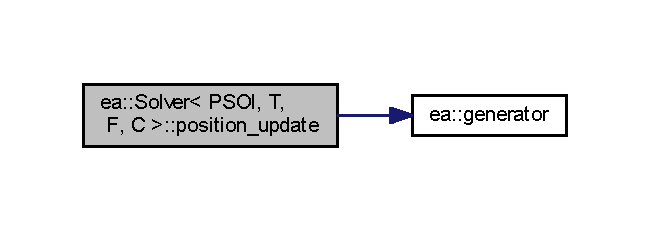
\includegraphics[width=312pt]{classea_1_1_solver_3_01_p_s_ol_00_01_t_00_01_f_00_01_c_01_4_a9f20cae513cb6a44dddc59ef43ee206f_cgraph}
\end{center}
\end{figure}
\mbox{\Hypertarget{classea_1_1_solver_3_01_p_s_ol_00_01_t_00_01_f_00_01_c_01_4_a0fa43e874bb60282a742c4c3dff651a9}\label{classea_1_1_solver_3_01_p_s_ol_00_01_t_00_01_f_00_01_c_01_4_a0fa43e874bb60282a742c4c3dff651a9}} 
\index{ea\+::\+Solver$<$ P\+S\+Ol, T, F, C $>$@{ea\+::\+Solver$<$ P\+S\+Ol, T, F, C $>$}!run\+\_\+algo@{run\+\_\+algo}}
\index{run\+\_\+algo@{run\+\_\+algo}!ea\+::\+Solver$<$ P\+S\+Ol, T, F, C $>$@{ea\+::\+Solver$<$ P\+S\+Ol, T, F, C $>$}}
\subsubsection{\texorpdfstring{run\+\_\+algo()}{run\_algo()}}
{\footnotesize\ttfamily template$<$typename T , typename F , typename C $>$ \\
void \hyperlink{classea_1_1_solver}{ea\+::\+Solver}$<$ \hyperlink{structea_1_1_p_s_ol}{P\+S\+Ol}, T, F, C $>$\+::run\+\_\+algo (\begin{DoxyParamCaption}{ }\end{DoxyParamCaption})\hspace{0.3cm}{\ttfamily [private]}}



Runs the algorithm until stopping criteria return void. 

Local Best Particle Swarm starts here

Inertia weight is updated -\/ Linear

Non-\/linear 

Definition at line 310 of file lbestpso.\+h.



References ea\+::\+P\+S\+Ol$<$ T $>$\+::w.


\begin{DoxyCode}
311     \{
313         \textcolor{keywordflow}{for} (\textcolor{keywordtype}{size\_t} iter = 0; iter < \hyperlink{classea_1_1_solver_3_01_p_s_ol_00_01_t_00_01_f_00_01_c_01_4_a3098f083ef04a0ce7ae0eef22dd80442}{pso}.iter\_max; ++iter)
314         \{
315             \hyperlink{classea_1_1_solver_3_01_p_s_ol_00_01_t_00_01_f_00_01_c_01_4_a9f20cae513cb6a44dddc59ef43ee206f}{position\_update}();
316             \textcolor{comment}{//best\_update();}
317             \hyperlink{classea_1_1_solver_3_01_p_s_ol_00_01_t_00_01_f_00_01_c_01_4_ae7821ee945e33732ec24d47c88d4b310}{find\_min\_local\_best}();
319             \textcolor{comment}{//w = pso.w - (pso.w - 0.4) * (static\_cast<T>(iter) / static\_cast<T>(pso.iter\_max));}
321 \textcolor{comment}{}            \hyperlink{classea_1_1_solver_3_01_p_s_ol_00_01_t_00_01_f_00_01_c_01_4_a5c9d1a207892da92e2cf689b24c256ee}{w} = \hyperlink{classea_1_1_solver_3_01_p_s_ol_00_01_t_00_01_f_00_01_c_01_4_a3098f083ef04a0ce7ae0eef22dd80442}{pso}.w - (\hyperlink{classea_1_1_solver_3_01_p_s_ol_00_01_t_00_01_f_00_01_c_01_4_a3098f083ef04a0ce7ae0eef22dd80442}{pso}.w - 0.4) * std::pow((static\_cast<T>(iter) / static\_cast<T>(
      \hyperlink{classea_1_1_solver_3_01_p_s_ol_00_01_t_00_01_f_00_01_c_01_4_a3098f083ef04a0ce7ae0eef22dd80442}{pso}.iter\_max)), inv\_pi\_sq<T>);
322             \textcolor{comment}{//w = 0.729;}
323             \textcolor{comment}{//w = 0.5 + distribution(generator) / 2;}
324             this->\hyperlink{classea_1_1_solver__base_a8f9a321eb87e57636cf0b0f3a57b6fc2}{last\_iter} = iter;
325             \textcolor{keywordflow}{if} (\hyperlink{classea_1_1_solver_3_01_p_s_ol_00_01_t_00_01_f_00_01_c_01_4_a474c18a8544f7ae0d5fe9d1587de2ad3}{check\_pso\_criteria}())
326             \{
327                 this->\hyperlink{classea_1_1_solver__base_a1cdb824e8df6d4a8f228820ea85c9b05}{solved\_flag} = \textcolor{keyword}{true};
328                 \textcolor{keywordflow}{break};
329             \}
330         \}
331     \}
\end{DoxyCode}
\mbox{\Hypertarget{classea_1_1_solver_3_01_p_s_ol_00_01_t_00_01_f_00_01_c_01_4_ae7599388d63b6905f4d9c49a3ad85387}\label{classea_1_1_solver_3_01_p_s_ol_00_01_t_00_01_f_00_01_c_01_4_ae7599388d63b6905f4d9c49a3ad85387}} 
\index{ea\+::\+Solver$<$ P\+S\+Ol, T, F, C $>$@{ea\+::\+Solver$<$ P\+S\+Ol, T, F, C $>$}!set\+\_\+neighbourhoods@{set\+\_\+neighbourhoods}}
\index{set\+\_\+neighbourhoods@{set\+\_\+neighbourhoods}!ea\+::\+Solver$<$ P\+S\+Ol, T, F, C $>$@{ea\+::\+Solver$<$ P\+S\+Ol, T, F, C $>$}}
\subsubsection{\texorpdfstring{set\+\_\+neighbourhoods()}{set\_neighbourhoods()}}
{\footnotesize\ttfamily template$<$typename T , typename F , typename C $>$ \\
std\+::unordered\+\_\+map$<$ size\+\_\+t, std\+::array$<$ size\+\_\+t, 3 $>$ $>$ \hyperlink{classea_1_1_solver}{ea\+::\+Solver}$<$ \hyperlink{structea_1_1_p_s_ol}{P\+S\+Ol}, T, F, C $>$\+::set\+\_\+neighbourhoods (\begin{DoxyParamCaption}{ }\end{DoxyParamCaption})\hspace{0.3cm}{\ttfamily [private]}}



Set the neighbourhoods of the algorithm using particle indices. 

\begin{DoxyReturn}{Returns}
A map matching particle indices to neighbourhoods 
\end{DoxyReturn}


Definition at line 196 of file lbestpso.\+h.


\begin{DoxyCode}
197     \{
198         std::unordered\_map<size\_t, std::array<size\_t, 3>> \hyperlink{classea_1_1_solver_3_01_p_s_ol_00_01_t_00_01_f_00_01_c_01_4_ab92e8a0460092b8264bd9023a3455257}{neighbours};
199         \textcolor{keywordflow}{for} (\textcolor{keywordtype}{size\_t} i = 0; i < \hyperlink{classea_1_1_solver_3_01_p_s_ol_00_01_t_00_01_f_00_01_c_01_4_a3098f083ef04a0ce7ae0eef22dd80442}{pso}.npop; ++i)
200         \{
201             \textcolor{keywordflow}{if} (i == 0)
202             \{
203                 neighbours[i] = \{ \hyperlink{classea_1_1_solver_3_01_p_s_ol_00_01_t_00_01_f_00_01_c_01_4_a3098f083ef04a0ce7ae0eef22dd80442}{pso}.npop - 1, i, i + 1 \};
204             \}
205             \textcolor{keywordflow}{else}
206             \{
207                 \textcolor{keywordflow}{if} (i == \hyperlink{classea_1_1_solver_3_01_p_s_ol_00_01_t_00_01_f_00_01_c_01_4_a3098f083ef04a0ce7ae0eef22dd80442}{pso}.npop - 1)
208                 \{
209                     neighbours[i] = \{ \hyperlink{classea_1_1_solver_3_01_p_s_ol_00_01_t_00_01_f_00_01_c_01_4_a3098f083ef04a0ce7ae0eef22dd80442}{pso}.npop - 2, i, 0 \};
210                 \}
211                 \textcolor{keywordflow}{else}
212                 \{
213                     neighbours[i] = \{ i - 1, i, i + 1 \};
214                 \}
215             \}
216         \}
217         \textcolor{keywordflow}{return} \hyperlink{classea_1_1_solver_3_01_p_s_ol_00_01_t_00_01_f_00_01_c_01_4_ab92e8a0460092b8264bd9023a3455257}{neighbours};
218     \}
\end{DoxyCode}


\subsection{Friends And Related Function Documentation}
\mbox{\Hypertarget{classea_1_1_solver_3_01_p_s_ol_00_01_t_00_01_f_00_01_c_01_4_a95bfc162c6509fec9ecb02185ed094d3}\label{classea_1_1_solver_3_01_p_s_ol_00_01_t_00_01_f_00_01_c_01_4_a95bfc162c6509fec9ecb02185ed094d3}} 
\index{ea\+::\+Solver$<$ P\+S\+Ol, T, F, C $>$@{ea\+::\+Solver$<$ P\+S\+Ol, T, F, C $>$}!Solver\+\_\+base$<$ Solver$<$ P\+S\+Ol, T, F, C $>$, P\+S\+Ol, T, F, C $>$@{Solver\+\_\+base$<$ Solver$<$ P\+S\+Ol, T, F, C $>$, P\+S\+Ol, T, F, C $>$}}
\index{Solver\+\_\+base$<$ Solver$<$ P\+S\+Ol, T, F, C $>$, P\+S\+Ol, T, F, C $>$@{Solver\+\_\+base$<$ Solver$<$ P\+S\+Ol, T, F, C $>$, P\+S\+Ol, T, F, C $>$}!ea\+::\+Solver$<$ P\+S\+Ol, T, F, C $>$@{ea\+::\+Solver$<$ P\+S\+Ol, T, F, C $>$}}
\subsubsection{\texorpdfstring{Solver\+\_\+base$<$ Solver$<$ P\+S\+Ol, T, F, C $>$, P\+S\+Ol, T, F, C $>$}{Solver\_base< Solver< PSOl, T, F, C >, PSOl, T, F, C >}}
{\footnotesize\ttfamily template$<$typename T , typename F , typename C $>$ \\
friend class \hyperlink{classea_1_1_solver__base}{Solver\+\_\+base}$<$ \hyperlink{classea_1_1_solver}{Solver}$<$ \hyperlink{structea_1_1_p_s_ol}{P\+S\+Ol}, T, F, C $>$, \hyperlink{structea_1_1_p_s_ol}{P\+S\+Ol}, T, F, C $>$\hspace{0.3cm}{\ttfamily [friend]}}



Definition at line 72 of file lbestpso.\+h.



\subsection{Member Data Documentation}
\mbox{\Hypertarget{classea_1_1_solver_3_01_p_s_ol_00_01_t_00_01_f_00_01_c_01_4_a6671c3d551564e3b4cd0944bfb2c33fd}\label{classea_1_1_solver_3_01_p_s_ol_00_01_t_00_01_f_00_01_c_01_4_a6671c3d551564e3b4cd0944bfb2c33fd}} 
\index{ea\+::\+Solver$<$ P\+S\+Ol, T, F, C $>$@{ea\+::\+Solver$<$ P\+S\+Ol, T, F, C $>$}!local\+\_\+best@{local\+\_\+best}}
\index{local\+\_\+best@{local\+\_\+best}!ea\+::\+Solver$<$ P\+S\+Ol, T, F, C $>$@{ea\+::\+Solver$<$ P\+S\+Ol, T, F, C $>$}}
\subsubsection{\texorpdfstring{local\+\_\+best}{local\_best}}
{\footnotesize\ttfamily template$<$typename T , typename F , typename C $>$ \\
std\+::vector$<$std\+::vector$<$T$>$ $>$ \hyperlink{classea_1_1_solver}{ea\+::\+Solver}$<$ \hyperlink{structea_1_1_p_s_ol}{P\+S\+Ol}, T, F, C $>$\+::local\+\_\+best\hspace{0.3cm}{\ttfamily [private]}}



Local best vector, holds the best position recorded for each neighbourhood. 



Definition at line 130 of file lbestpso.\+h.

\mbox{\Hypertarget{classea_1_1_solver_3_01_p_s_ol_00_01_t_00_01_f_00_01_c_01_4_ab92e8a0460092b8264bd9023a3455257}\label{classea_1_1_solver_3_01_p_s_ol_00_01_t_00_01_f_00_01_c_01_4_ab92e8a0460092b8264bd9023a3455257}} 
\index{ea\+::\+Solver$<$ P\+S\+Ol, T, F, C $>$@{ea\+::\+Solver$<$ P\+S\+Ol, T, F, C $>$}!neighbours@{neighbours}}
\index{neighbours@{neighbours}!ea\+::\+Solver$<$ P\+S\+Ol, T, F, C $>$@{ea\+::\+Solver$<$ P\+S\+Ol, T, F, C $>$}}
\subsubsection{\texorpdfstring{neighbours}{neighbours}}
{\footnotesize\ttfamily template$<$typename T , typename F , typename C $>$ \\
std\+::unordered\+\_\+map$<$size\+\_\+t, std\+::array$<$size\+\_\+t, 3$>$ $>$ \hyperlink{classea_1_1_solver}{ea\+::\+Solver}$<$ \hyperlink{structea_1_1_p_s_ol}{P\+S\+Ol}, T, F, C $>$\+::neighbours\hspace{0.3cm}{\ttfamily [private]}}



Neighbours of each particle. 



Definition at line 136 of file lbestpso.\+h.

\mbox{\Hypertarget{classea_1_1_solver_3_01_p_s_ol_00_01_t_00_01_f_00_01_c_01_4_adb34cfcd87307ee2271b5aa5ffdd779d}\label{classea_1_1_solver_3_01_p_s_ol_00_01_t_00_01_f_00_01_c_01_4_adb34cfcd87307ee2271b5aa5ffdd779d}} 
\index{ea\+::\+Solver$<$ P\+S\+Ol, T, F, C $>$@{ea\+::\+Solver$<$ P\+S\+Ol, T, F, C $>$}!nneigh@{nneigh}}
\index{nneigh@{nneigh}!ea\+::\+Solver$<$ P\+S\+Ol, T, F, C $>$@{ea\+::\+Solver$<$ P\+S\+Ol, T, F, C $>$}}
\subsubsection{\texorpdfstring{nneigh}{nneigh}}
{\footnotesize\ttfamily template$<$typename T , typename F , typename C $>$ \\
const size\+\_\+t \hyperlink{classea_1_1_solver}{ea\+::\+Solver}$<$ \hyperlink{structea_1_1_p_s_ol}{P\+S\+Ol}, T, F, C $>$\+::nneigh\hspace{0.3cm}{\ttfamily [private]}}



Number of neighbourhoods. 



Definition at line 134 of file lbestpso.\+h.

\mbox{\Hypertarget{classea_1_1_solver_3_01_p_s_ol_00_01_t_00_01_f_00_01_c_01_4_a0738e0ab079273c4d34c827fad533868}\label{classea_1_1_solver_3_01_p_s_ol_00_01_t_00_01_f_00_01_c_01_4_a0738e0ab079273c4d34c827fad533868}} 
\index{ea\+::\+Solver$<$ P\+S\+Ol, T, F, C $>$@{ea\+::\+Solver$<$ P\+S\+Ol, T, F, C $>$}!personal\+\_\+best@{personal\+\_\+best}}
\index{personal\+\_\+best@{personal\+\_\+best}!ea\+::\+Solver$<$ P\+S\+Ol, T, F, C $>$@{ea\+::\+Solver$<$ P\+S\+Ol, T, F, C $>$}}
\subsubsection{\texorpdfstring{personal\+\_\+best}{personal\_best}}
{\footnotesize\ttfamily template$<$typename T , typename F , typename C $>$ \\
std\+::vector$<$std\+::vector$<$T$>$ $>$ \hyperlink{classea_1_1_solver}{ea\+::\+Solver}$<$ \hyperlink{structea_1_1_p_s_ol}{P\+S\+Ol}, T, F, C $>$\+::personal\+\_\+best\hspace{0.3cm}{\ttfamily [private]}}



Personal best vector of the particles, holds the best position recorded for each particle. 



Definition at line 126 of file lbestpso.\+h.

\mbox{\Hypertarget{classea_1_1_solver_3_01_p_s_ol_00_01_t_00_01_f_00_01_c_01_4_ae728d584641709062919b0cedd3e77cc}\label{classea_1_1_solver_3_01_p_s_ol_00_01_t_00_01_f_00_01_c_01_4_ae728d584641709062919b0cedd3e77cc}} 
\index{ea\+::\+Solver$<$ P\+S\+Ol, T, F, C $>$@{ea\+::\+Solver$<$ P\+S\+Ol, T, F, C $>$}!personal\+\_\+best\+\_\+cost@{personal\+\_\+best\+\_\+cost}}
\index{personal\+\_\+best\+\_\+cost@{personal\+\_\+best\+\_\+cost}!ea\+::\+Solver$<$ P\+S\+Ol, T, F, C $>$@{ea\+::\+Solver$<$ P\+S\+Ol, T, F, C $>$}}
\subsubsection{\texorpdfstring{personal\+\_\+best\+\_\+cost}{personal\_best\_cost}}
{\footnotesize\ttfamily template$<$typename T , typename F , typename C $>$ \\
std\+::vector$<$T$>$ \hyperlink{classea_1_1_solver}{ea\+::\+Solver}$<$ \hyperlink{structea_1_1_p_s_ol}{P\+S\+Ol}, T, F, C $>$\+::personal\+\_\+best\+\_\+cost\hspace{0.3cm}{\ttfamily [private]}}



Personal best cost vector of the particles. 



Definition at line 128 of file lbestpso.\+h.

\mbox{\Hypertarget{classea_1_1_solver_3_01_p_s_ol_00_01_t_00_01_f_00_01_c_01_4_a3098f083ef04a0ce7ae0eef22dd80442}\label{classea_1_1_solver_3_01_p_s_ol_00_01_t_00_01_f_00_01_c_01_4_a3098f083ef04a0ce7ae0eef22dd80442}} 
\index{ea\+::\+Solver$<$ P\+S\+Ol, T, F, C $>$@{ea\+::\+Solver$<$ P\+S\+Ol, T, F, C $>$}!pso@{pso}}
\index{pso@{pso}!ea\+::\+Solver$<$ P\+S\+Ol, T, F, C $>$@{ea\+::\+Solver$<$ P\+S\+Ol, T, F, C $>$}}
\subsubsection{\texorpdfstring{pso}{pso}}
{\footnotesize\ttfamily template$<$typename T , typename F , typename C $>$ \\
const \hyperlink{structea_1_1_p_s_ol}{P\+S\+Ol}$<$T$>$\& \hyperlink{classea_1_1_solver}{ea\+::\+Solver}$<$ \hyperlink{structea_1_1_p_s_ol}{P\+S\+Ol}, T, F, C $>$\+::pso\hspace{0.3cm}{\ttfamily [private]}}



Particle Swarm Optimisation structure used internally (reference to solver\+\_\+struct) 



Definition at line 120 of file lbestpso.\+h.

\mbox{\Hypertarget{classea_1_1_solver_3_01_p_s_ol_00_01_t_00_01_f_00_01_c_01_4_ae8293610cb6bffc00e0fda749754a1f2}\label{classea_1_1_solver_3_01_p_s_ol_00_01_t_00_01_f_00_01_c_01_4_ae8293610cb6bffc00e0fda749754a1f2}} 
\index{ea\+::\+Solver$<$ P\+S\+Ol, T, F, C $>$@{ea\+::\+Solver$<$ P\+S\+Ol, T, F, C $>$}!velocity@{velocity}}
\index{velocity@{velocity}!ea\+::\+Solver$<$ P\+S\+Ol, T, F, C $>$@{ea\+::\+Solver$<$ P\+S\+Ol, T, F, C $>$}}
\subsubsection{\texorpdfstring{velocity}{velocity}}
{\footnotesize\ttfamily template$<$typename T , typename F , typename C $>$ \\
std\+::vector$<$std\+::vector$<$T$>$ $>$ \hyperlink{classea_1_1_solver}{ea\+::\+Solver}$<$ \hyperlink{structea_1_1_p_s_ol}{P\+S\+Ol}, T, F, C $>$\+::velocity\hspace{0.3cm}{\ttfamily [private]}}



Velocity of the particles. 



Definition at line 132 of file lbestpso.\+h.

\mbox{\Hypertarget{classea_1_1_solver_3_01_p_s_ol_00_01_t_00_01_f_00_01_c_01_4_abd93da2229dac4eb2d11f4904a65ae9a}\label{classea_1_1_solver_3_01_p_s_ol_00_01_t_00_01_f_00_01_c_01_4_abd93da2229dac4eb2d11f4904a65ae9a}} 
\index{ea\+::\+Solver$<$ P\+S\+Ol, T, F, C $>$@{ea\+::\+Solver$<$ P\+S\+Ol, T, F, C $>$}!vmax@{vmax}}
\index{vmax@{vmax}!ea\+::\+Solver$<$ P\+S\+Ol, T, F, C $>$@{ea\+::\+Solver$<$ P\+S\+Ol, T, F, C $>$}}
\subsubsection{\texorpdfstring{vmax}{vmax}}
{\footnotesize\ttfamily template$<$typename T , typename F , typename C $>$ \\
std\+::vector$<$T$>$ \hyperlink{classea_1_1_solver}{ea\+::\+Solver}$<$ \hyperlink{structea_1_1_p_s_ol}{P\+S\+Ol}, T, F, C $>$\+::vmax\hspace{0.3cm}{\ttfamily [private]}}



Maximum Velocity is mutable, so a copy is created. 



Definition at line 124 of file lbestpso.\+h.

\mbox{\Hypertarget{classea_1_1_solver_3_01_p_s_ol_00_01_t_00_01_f_00_01_c_01_4_a5c9d1a207892da92e2cf689b24c256ee}\label{classea_1_1_solver_3_01_p_s_ol_00_01_t_00_01_f_00_01_c_01_4_a5c9d1a207892da92e2cf689b24c256ee}} 
\index{ea\+::\+Solver$<$ P\+S\+Ol, T, F, C $>$@{ea\+::\+Solver$<$ P\+S\+Ol, T, F, C $>$}!w@{w}}
\index{w@{w}!ea\+::\+Solver$<$ P\+S\+Ol, T, F, C $>$@{ea\+::\+Solver$<$ P\+S\+Ol, T, F, C $>$}}
\subsubsection{\texorpdfstring{w}{w}}
{\footnotesize\ttfamily template$<$typename T , typename F , typename C $>$ \\
T \hyperlink{classea_1_1_solver}{ea\+::\+Solver}$<$ \hyperlink{structea_1_1_p_s_ol}{P\+S\+Ol}, T, F, C $>$\+::w\hspace{0.3cm}{\ttfamily [private]}}



Inertia is mutable, so a copy is created. 



Definition at line 122 of file lbestpso.\+h.



The documentation for this class was generated from the following file\+:\begin{DoxyCompactItemize}
\item 
\hyperlink{lbestpso_8h}{lbestpso.\+h}\end{DoxyCompactItemize}

\hypertarget{classea_1_1_solver_3_01_p_s_os_00_01_t_00_01_f_00_01_c_01_4}{}\section{ea\+:\+:Solver$<$ P\+S\+Os, T, F, C $>$ Class Template Reference}
\label{classea_1_1_solver_3_01_p_s_os_00_01_t_00_01_f_00_01_c_01_4}\index{ea\+::\+Solver$<$ P\+S\+Os, T, F, C $>$@{ea\+::\+Solver$<$ P\+S\+Os, T, F, C $>$}}


Sub-\/\+Swarm Particle Swarm Optimisation (P\+SO) Class.  




{\ttfamily \#include $<$pso\+\_\+sub\+\_\+swarm.\+h$>$}



Inheritance diagram for ea\+:\+:Solver$<$ P\+S\+Os, T, F, C $>$\+:
\nopagebreak
\begin{figure}[H]
\begin{center}
\leavevmode
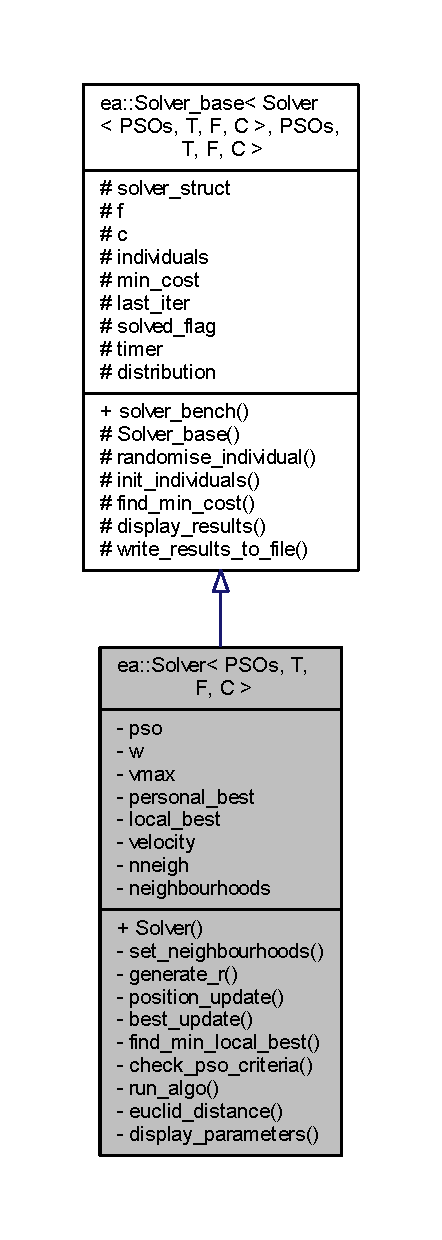
\includegraphics[height=550pt]{classea_1_1_solver_3_01_p_s_os_00_01_t_00_01_f_00_01_c_01_4__inherit__graph}
\end{center}
\end{figure}
\subsection*{Public Member Functions}
\begin{DoxyCompactItemize}
\item 
\hyperlink{classea_1_1_solver_3_01_p_s_os_00_01_t_00_01_f_00_01_c_01_4_a221b61b8df52b5d3d23a31e230d39f0d}{Solver} (const \hyperlink{structea_1_1_p_s_os}{P\+S\+Os}$<$ T $>$ \&i\+\_\+pso, F \hyperlink{classea_1_1_solver__base_ae0a893780c93dfe17c1d17301de6494f}{f}, C \hyperlink{classea_1_1_solver__base_a6914e89d30e7484f2b4af1783f0de8c3}{c})
\begin{DoxyCompactList}\small\item\em Constructor. \end{DoxyCompactList}\end{DoxyCompactItemize}
\subsection*{Private Member Functions}
\begin{DoxyCompactItemize}
\item 
std\+::unordered\+\_\+map$<$ size\+\_\+t, size\+\_\+t $>$ \hyperlink{classea_1_1_solver_3_01_p_s_os_00_01_t_00_01_f_00_01_c_01_4_acf9a10b2f3e095c365fa787c06709a3d}{set\+\_\+neighbourhoods} ()
\begin{DoxyCompactList}\small\item\em Set the neighbourhoods of the algorithm using particle indices. \end{DoxyCompactList}\item 
std\+::vector$<$ std\+::vector$<$ T $>$ $>$ \hyperlink{classea_1_1_solver_3_01_p_s_os_00_01_t_00_01_f_00_01_c_01_4_a01ea94eec2b6f05c62c9f83d725bb75b}{generate\+\_\+r} ()
\begin{DoxyCompactList}\small\item\em This method generates r1 and r2 for the velocity update rule. \end{DoxyCompactList}\item 
void \hyperlink{classea_1_1_solver_3_01_p_s_os_00_01_t_00_01_f_00_01_c_01_4_a91feb28b5a3b292da8eedb1f782d53c0}{position\+\_\+update} ()
\begin{DoxyCompactList}\small\item\em Position update of the particles. \end{DoxyCompactList}\item 
void \hyperlink{classea_1_1_solver_3_01_p_s_os_00_01_t_00_01_f_00_01_c_01_4_ab52c41eb3bea4aa9465ff254bee82990}{best\+\_\+update} ()
\begin{DoxyCompactList}\small\item\em This method sets the personal and local best solutions. \end{DoxyCompactList}\item 
void \hyperlink{classea_1_1_solver_3_01_p_s_os_00_01_t_00_01_f_00_01_c_01_4_a012b67607139916c790167fefc1f38e7}{find\+\_\+min\+\_\+local\+\_\+best} ()
\begin{DoxyCompactList}\small\item\em This is a faster way to calculate the minimum cost unless there is only one neighbourhood, in which case it is the same as find\+\_\+min\+\_\+cost(\+F f) \end{DoxyCompactList}\item 
bool \hyperlink{classea_1_1_solver_3_01_p_s_os_00_01_t_00_01_f_00_01_c_01_4_afd7a166bcdc0730431ca9406f0d0e030}{check\+\_\+pso\+\_\+criteria} ()
\begin{DoxyCompactList}\small\item\em Define the maximum radius stopping criterion. \end{DoxyCompactList}\item 
void \hyperlink{classea_1_1_solver_3_01_p_s_os_00_01_t_00_01_f_00_01_c_01_4_a4952777e6e95820c9702e9306e24d1fb}{run\+\_\+algo} ()
\begin{DoxyCompactList}\small\item\em Runs the algorithm until stopping criteria return void. \end{DoxyCompactList}\item 
T \hyperlink{classea_1_1_solver_3_01_p_s_os_00_01_t_00_01_f_00_01_c_01_4_abb67d82749ba9525e7c8c68f5494389f}{euclid\+\_\+distance} (const std\+::vector$<$ T $>$ \&x, const std\+::vector$<$ T $>$ \&y)
\begin{DoxyCompactList}\small\item\em Euclidean Distance of two vectors .. \end{DoxyCompactList}\item 
std\+::stringstream \hyperlink{classea_1_1_solver_3_01_p_s_os_00_01_t_00_01_f_00_01_c_01_4_afcb113cca952b4954e3639e538d6c5cd}{display\+\_\+parameters} ()
\begin{DoxyCompactList}\small\item\em Display P\+SO parameters. \end{DoxyCompactList}\end{DoxyCompactItemize}
\subsection*{Private Attributes}
\begin{DoxyCompactItemize}
\item 
const \hyperlink{structea_1_1_p_s_os}{P\+S\+Os}$<$ T $>$ \& \hyperlink{classea_1_1_solver_3_01_p_s_os_00_01_t_00_01_f_00_01_c_01_4_a1f1aa62756a73565ebe0ca1fbc084ea5}{pso}
\begin{DoxyCompactList}\small\item\em Particle Swarm Optimisation structure used internally (reference to solver\+\_\+struct) \end{DoxyCompactList}\item 
T \hyperlink{classea_1_1_solver_3_01_p_s_os_00_01_t_00_01_f_00_01_c_01_4_a4f690e68bf36069ba446ef96b03da6f6}{w}
\begin{DoxyCompactList}\small\item\em Inertia is mutable, so a copy is created. \end{DoxyCompactList}\item 
std\+::vector$<$ T $>$ \hyperlink{classea_1_1_solver_3_01_p_s_os_00_01_t_00_01_f_00_01_c_01_4_ade5fde673b93afeb9e3cb410d6f1061a}{vmax}
\begin{DoxyCompactList}\small\item\em Maximum Velocity is mutable, so a copy is created. \end{DoxyCompactList}\item 
std\+::vector$<$ std\+::vector$<$ T $>$ $>$ \hyperlink{classea_1_1_solver_3_01_p_s_os_00_01_t_00_01_f_00_01_c_01_4_a8a857e38363bd1ed23ea77e262b9b710}{personal\+\_\+best}
\begin{DoxyCompactList}\small\item\em Personal best vector of the particles, holds the best position recorded for each particle. \end{DoxyCompactList}\item 
std\+::vector$<$ std\+::vector$<$ T $>$ $>$ \hyperlink{classea_1_1_solver_3_01_p_s_os_00_01_t_00_01_f_00_01_c_01_4_afa2eb13f0e5028ba4aa96f7e29b62e9c}{local\+\_\+best}
\begin{DoxyCompactList}\small\item\em Local best vector, holds the best position recorded for each neighbourhood. \end{DoxyCompactList}\item 
std\+::vector$<$ std\+::vector$<$ T $>$ $>$ \hyperlink{classea_1_1_solver_3_01_p_s_os_00_01_t_00_01_f_00_01_c_01_4_ac188af95a817ad70538969bd5af2dc66}{velocity}
\begin{DoxyCompactList}\small\item\em Velocity of the particles. \end{DoxyCompactList}\item 
const size\+\_\+t \hyperlink{classea_1_1_solver_3_01_p_s_os_00_01_t_00_01_f_00_01_c_01_4_a92980b9d3411dd8855a6a050722ebcf7}{nneigh}
\begin{DoxyCompactList}\small\item\em Number of neighbourhoods. \end{DoxyCompactList}\item 
std\+::unordered\+\_\+map$<$ size\+\_\+t, size\+\_\+t $>$ \hyperlink{classea_1_1_solver_3_01_p_s_os_00_01_t_00_01_f_00_01_c_01_4_a192926bdbed79d0cd68867c4f695cd92}{neighbourhoods}
\begin{DoxyCompactList}\small\item\em Neighbourhoods. \end{DoxyCompactList}\end{DoxyCompactItemize}
\subsection*{Friends}
\begin{DoxyCompactItemize}
\item 
class \hyperlink{classea_1_1_solver_3_01_p_s_os_00_01_t_00_01_f_00_01_c_01_4_aa3dcae3fc6bad98284e958b7c320549c}{Solver\+\_\+base$<$ Solver$<$ P\+S\+Os, T, F, C $>$, P\+S\+Os, T, F, C $>$}
\end{DoxyCompactItemize}
\subsection*{Additional Inherited Members}


\subsection{Detailed Description}
\subsubsection*{template$<$typename T, typename F, typename C$>$\newline
class ea\+::\+Solver$<$ P\+S\+Os, T, F, C $>$}

Sub-\/\+Swarm Particle Swarm Optimisation (P\+SO) Class. 

Definition at line 83 of file pso\+\_\+sub\+\_\+swarm.\+h.



\subsection{Constructor \& Destructor Documentation}
\mbox{\Hypertarget{classea_1_1_solver_3_01_p_s_os_00_01_t_00_01_f_00_01_c_01_4_a221b61b8df52b5d3d23a31e230d39f0d}\label{classea_1_1_solver_3_01_p_s_os_00_01_t_00_01_f_00_01_c_01_4_a221b61b8df52b5d3d23a31e230d39f0d}} 
\index{ea\+::\+Solver$<$ P\+S\+Os, T, F, C $>$@{ea\+::\+Solver$<$ P\+S\+Os, T, F, C $>$}!Solver@{Solver}}
\index{Solver@{Solver}!ea\+::\+Solver$<$ P\+S\+Os, T, F, C $>$@{ea\+::\+Solver$<$ P\+S\+Os, T, F, C $>$}}
\subsubsection{\texorpdfstring{Solver()}{Solver()}}
{\footnotesize\ttfamily template$<$typename T , typename F , typename C $>$ \\
\hyperlink{classea_1_1_solver}{ea\+::\+Solver}$<$ \hyperlink{structea_1_1_p_s_os}{P\+S\+Os}, T, F, C $>$\+::\hyperlink{classea_1_1_solver}{Solver} (\begin{DoxyParamCaption}\item[{const \hyperlink{structea_1_1_p_s_os}{P\+S\+Os}$<$ T $>$ \&}]{i\+\_\+pso,  }\item[{F}]{f,  }\item[{C}]{c }\end{DoxyParamCaption})\hspace{0.3cm}{\ttfamily [inline]}}



Constructor. 


\begin{DoxyParams}{Parameters}
{\em i\+\_\+pso} & The particle swarm optimisation parameter structure that is used to construct the solver \\
\hline
{\em f} & A reference to the objective function \\
\hline
{\em c} & A reference to the constraints function \\
\hline
\end{DoxyParams}
\begin{DoxyReturn}{Returns}
A \hyperlink{classea_1_1_solver_3_01_p_s_os_00_01_t_00_01_f_00_01_c_01_4}{Solver$<$\+P\+S\+Os, T, F, C$>$} object 
\end{DoxyReturn}


Definition at line 94 of file pso\+\_\+sub\+\_\+swarm.\+h.


\begin{DoxyCode}
94                                                :
95             Solver\_base<Solver<PSOs, T, F, C>, PSOs, T, F, C>( i\_pso, \hyperlink{classea_1_1_solver__base_ae0a893780c93dfe17c1d17301de6494f}{f}, \hyperlink{classea_1_1_solver__base_a6914e89d30e7484f2b4af1783f0de8c3}{c} ),
96             \hyperlink{classea_1_1_solver_3_01_p_s_os_00_01_t_00_01_f_00_01_c_01_4_a1f1aa62756a73565ebe0ca1fbc084ea5}{pso}( this->\hyperlink{classea_1_1_solver__base_a5e1d821809f2d26c6f882942ad728127}{solver\_struct} ), 
97             \hyperlink{classea_1_1_solver_3_01_p_s_os_00_01_t_00_01_f_00_01_c_01_4_a4f690e68bf36069ba446ef96b03da6f6}{w}( i\_pso.w ), 
98             \hyperlink{classea_1_1_solver_3_01_p_s_os_00_01_t_00_01_f_00_01_c_01_4_ade5fde673b93afeb9e3cb410d6f1061a}{vmax}( i\_pso.vmax ),
99             \hyperlink{classea_1_1_solver_3_01_p_s_os_00_01_t_00_01_f_00_01_c_01_4_a92980b9d3411dd8855a6a050722ebcf7}{nneigh}( static\_cast<size\_t>(std::ceil(i\_pso.npop / i\_pso.sneigh)) ),
100             \hyperlink{classea_1_1_solver_3_01_p_s_os_00_01_t_00_01_f_00_01_c_01_4_a192926bdbed79d0cd68867c4f695cd92}{neighbourhoods}( \hyperlink{classea_1_1_solver_3_01_p_s_os_00_01_t_00_01_f_00_01_c_01_4_acf9a10b2f3e095c365fa787c06709a3d}{set\_neighbourhoods}() )
101         \{
102             \hyperlink{classea_1_1_solver_3_01_p_s_os_00_01_t_00_01_f_00_01_c_01_4_ac188af95a817ad70538969bd5af2dc66}{velocity}.resize(\hyperlink{classea_1_1_solver_3_01_p_s_os_00_01_t_00_01_f_00_01_c_01_4_a1f1aa62756a73565ebe0ca1fbc084ea5}{pso}.npop, std::vector<T>(\hyperlink{classea_1_1_solver_3_01_p_s_os_00_01_t_00_01_f_00_01_c_01_4_a1f1aa62756a73565ebe0ca1fbc084ea5}{pso}.ndv));
103             \hyperlink{classea_1_1_solver_3_01_p_s_os_00_01_t_00_01_f_00_01_c_01_4_afa2eb13f0e5028ba4aa96f7e29b62e9c}{local\_best}.resize(\hyperlink{classea_1_1_solver_3_01_p_s_os_00_01_t_00_01_f_00_01_c_01_4_a92980b9d3411dd8855a6a050722ebcf7}{nneigh});
104             \textcolor{keywordflow}{for} (\textcolor{keyword}{auto}& p : \hyperlink{classea_1_1_solver_3_01_p_s_os_00_01_t_00_01_f_00_01_c_01_4_ac188af95a817ad70538969bd5af2dc66}{velocity})
105             \{
106                 \textcolor{keywordflow}{for} (\textcolor{keyword}{auto}& n : p)
107                 \{
108                     n = 0.0;
109                 \}
110             \}
111             \textcolor{keywordflow}{for} (\textcolor{keyword}{const} \textcolor{keyword}{auto}& p : this->\hyperlink{classea_1_1_solver__base_ad75bc440d24a46e97694c7c889f2ecde}{individuals})
112             \{
113                 \hyperlink{classea_1_1_solver_3_01_p_s_os_00_01_t_00_01_f_00_01_c_01_4_a8a857e38363bd1ed23ea77e262b9b710}{personal\_best}.push\_back(p);
114             \}
115             \textcolor{keywordflow}{for} (\textcolor{keyword}{auto}& p : \hyperlink{classea_1_1_solver_3_01_p_s_os_00_01_t_00_01_f_00_01_c_01_4_afa2eb13f0e5028ba4aa96f7e29b62e9c}{local\_best})
116             \{
117                 p = \hyperlink{classea_1_1_solver_3_01_p_s_os_00_01_t_00_01_f_00_01_c_01_4_a8a857e38363bd1ed23ea77e262b9b710}{personal\_best}[0];
118             \}
119             \textcolor{keywordflow}{for} (\textcolor{keywordtype}{size\_t} i = 0; i < \hyperlink{classea_1_1_solver_3_01_p_s_os_00_01_t_00_01_f_00_01_c_01_4_a1f1aa62756a73565ebe0ca1fbc084ea5}{pso}.npop; ++i)
120             \{
121                 \textcolor{keywordflow}{if} (\hyperlink{classea_1_1_solver__base_ae0a893780c93dfe17c1d17301de6494f}{f}(\hyperlink{classea_1_1_solver_3_01_p_s_os_00_01_t_00_01_f_00_01_c_01_4_a8a857e38363bd1ed23ea77e262b9b710}{personal\_best}[i]) < \hyperlink{classea_1_1_solver__base_ae0a893780c93dfe17c1d17301de6494f}{f}(local\_best[
      \hyperlink{classea_1_1_solver_3_01_p_s_os_00_01_t_00_01_f_00_01_c_01_4_a192926bdbed79d0cd68867c4f695cd92}{neighbourhoods}[i]]))
122                 \{
123                     local\_best[\hyperlink{classea_1_1_solver_3_01_p_s_os_00_01_t_00_01_f_00_01_c_01_4_a192926bdbed79d0cd68867c4f695cd92}{neighbourhoods}[i]] = \hyperlink{classea_1_1_solver_3_01_p_s_os_00_01_t_00_01_f_00_01_c_01_4_a8a857e38363bd1ed23ea77e262b9b710}{personal\_best}[i];
124                 \}
125             \}
126             \hyperlink{classea_1_1_solver_3_01_p_s_os_00_01_t_00_01_f_00_01_c_01_4_a012b67607139916c790167fefc1f38e7}{find\_min\_local\_best}();
127         \}
\end{DoxyCode}


\subsection{Member Function Documentation}
\mbox{\Hypertarget{classea_1_1_solver_3_01_p_s_os_00_01_t_00_01_f_00_01_c_01_4_ab52c41eb3bea4aa9465ff254bee82990}\label{classea_1_1_solver_3_01_p_s_os_00_01_t_00_01_f_00_01_c_01_4_ab52c41eb3bea4aa9465ff254bee82990}} 
\index{ea\+::\+Solver$<$ P\+S\+Os, T, F, C $>$@{ea\+::\+Solver$<$ P\+S\+Os, T, F, C $>$}!best\+\_\+update@{best\+\_\+update}}
\index{best\+\_\+update@{best\+\_\+update}!ea\+::\+Solver$<$ P\+S\+Os, T, F, C $>$@{ea\+::\+Solver$<$ P\+S\+Os, T, F, C $>$}}
\subsubsection{\texorpdfstring{best\+\_\+update()}{best\_update()}}
{\footnotesize\ttfamily template$<$typename T , typename F , typename C $>$ \\
void \hyperlink{classea_1_1_solver}{ea\+::\+Solver}$<$ \hyperlink{structea_1_1_p_s_os}{P\+S\+Os}, T, F, C $>$\+::best\+\_\+update (\begin{DoxyParamCaption}{ }\end{DoxyParamCaption})\hspace{0.3cm}{\ttfamily [private]}}



This method sets the personal and local best solutions. 

\begin{DoxyReturn}{Returns}
void 
\end{DoxyReturn}
Checks that the candidate is feasible 

Definition at line 268 of file pso\+\_\+sub\+\_\+swarm.\+h.


\begin{DoxyCode}
269     \{
270         \textcolor{keywordflow}{for} (\textcolor{keywordtype}{size\_t} i = 0; i < \hyperlink{classea_1_1_solver_3_01_p_s_os_00_01_t_00_01_f_00_01_c_01_4_a1f1aa62756a73565ebe0ca1fbc084ea5}{pso}.npop; ++i)
271         \{
273             \textcolor{keywordflow}{if} (!this->\hyperlink{classea_1_1_solver__base_a6914e89d30e7484f2b4af1783f0de8c3}{c}(this->\hyperlink{classea_1_1_solver__base_ad75bc440d24a46e97694c7c889f2ecde}{individuals}[i]))
274             \{
275                 this->\hyperlink{classea_1_1_solver__base_ad75bc440d24a46e97694c7c889f2ecde}{individuals}[i] = \hyperlink{classea_1_1_solver_3_01_p_s_os_00_01_t_00_01_f_00_01_c_01_4_a8a857e38363bd1ed23ea77e262b9b710}{personal\_best}[i];
276             \}
277             \textcolor{keywordflow}{if} (this->\hyperlink{classea_1_1_solver__base_ae0a893780c93dfe17c1d17301de6494f}{f}(this->\hyperlink{classea_1_1_solver__base_ad75bc440d24a46e97694c7c889f2ecde}{individuals}[i]) < this->\hyperlink{classea_1_1_solver__base_ae0a893780c93dfe17c1d17301de6494f}{f}(
      \hyperlink{classea_1_1_solver_3_01_p_s_os_00_01_t_00_01_f_00_01_c_01_4_a8a857e38363bd1ed23ea77e262b9b710}{personal\_best}[i]))
278             \{
279                 \hyperlink{classea_1_1_solver_3_01_p_s_os_00_01_t_00_01_f_00_01_c_01_4_a8a857e38363bd1ed23ea77e262b9b710}{personal\_best}[i] = this->\hyperlink{classea_1_1_solver__base_ad75bc440d24a46e97694c7c889f2ecde}{individuals}[i];
280             \}
281             \textcolor{keywordflow}{if} (this->\hyperlink{classea_1_1_solver__base_ae0a893780c93dfe17c1d17301de6494f}{f}(\hyperlink{classea_1_1_solver_3_01_p_s_os_00_01_t_00_01_f_00_01_c_01_4_a8a857e38363bd1ed23ea77e262b9b710}{personal\_best}[i]) < this->\hyperlink{classea_1_1_solver__base_ae0a893780c93dfe17c1d17301de6494f}{f}(\hyperlink{classea_1_1_solver_3_01_p_s_os_00_01_t_00_01_f_00_01_c_01_4_afa2eb13f0e5028ba4aa96f7e29b62e9c}{local\_best}[
      \hyperlink{classea_1_1_solver_3_01_p_s_os_00_01_t_00_01_f_00_01_c_01_4_a192926bdbed79d0cd68867c4f695cd92}{neighbourhoods}[i]]))
282             \{
283                 \hyperlink{classea_1_1_solver_3_01_p_s_os_00_01_t_00_01_f_00_01_c_01_4_afa2eb13f0e5028ba4aa96f7e29b62e9c}{local\_best}[\hyperlink{classea_1_1_solver_3_01_p_s_os_00_01_t_00_01_f_00_01_c_01_4_a192926bdbed79d0cd68867c4f695cd92}{neighbourhoods}[i]] = 
      \hyperlink{classea_1_1_solver_3_01_p_s_os_00_01_t_00_01_f_00_01_c_01_4_a8a857e38363bd1ed23ea77e262b9b710}{personal\_best}[i];
284             \}
285         \}
286     \}
\end{DoxyCode}
\mbox{\Hypertarget{classea_1_1_solver_3_01_p_s_os_00_01_t_00_01_f_00_01_c_01_4_afd7a166bcdc0730431ca9406f0d0e030}\label{classea_1_1_solver_3_01_p_s_os_00_01_t_00_01_f_00_01_c_01_4_afd7a166bcdc0730431ca9406f0d0e030}} 
\index{ea\+::\+Solver$<$ P\+S\+Os, T, F, C $>$@{ea\+::\+Solver$<$ P\+S\+Os, T, F, C $>$}!check\+\_\+pso\+\_\+criteria@{check\+\_\+pso\+\_\+criteria}}
\index{check\+\_\+pso\+\_\+criteria@{check\+\_\+pso\+\_\+criteria}!ea\+::\+Solver$<$ P\+S\+Os, T, F, C $>$@{ea\+::\+Solver$<$ P\+S\+Os, T, F, C $>$}}
\subsubsection{\texorpdfstring{check\+\_\+pso\+\_\+criteria()}{check\_pso\_criteria()}}
{\footnotesize\ttfamily template$<$typename T , typename F , typename C $>$ \\
bool \hyperlink{classea_1_1_solver}{ea\+::\+Solver}$<$ \hyperlink{structea_1_1_p_s_os}{P\+S\+Os}, T, F, C $>$\+::check\+\_\+pso\+\_\+criteria (\begin{DoxyParamCaption}{ }\end{DoxyParamCaption})\hspace{0.3cm}{\ttfamily [private]}}



Define the maximum radius stopping criterion. 

\begin{DoxyReturn}{Returns}
true if criteria are met, false otherwise 
\end{DoxyReturn}


Definition at line 301 of file pso\+\_\+sub\+\_\+swarm.\+h.


\begin{DoxyCode}
302     \{
303         std::vector<T> distance(\hyperlink{classea_1_1_solver_3_01_p_s_os_00_01_t_00_01_f_00_01_c_01_4_a1f1aa62756a73565ebe0ca1fbc084ea5}{pso}.npop);
304         \textcolor{keywordflow}{for} (\textcolor{keywordtype}{size\_t} i = 0; i < \hyperlink{classea_1_1_solver_3_01_p_s_os_00_01_t_00_01_f_00_01_c_01_4_a1f1aa62756a73565ebe0ca1fbc084ea5}{pso}.npop; ++i)
305         \{
306             distance[i] = \hyperlink{classea_1_1_solver_3_01_p_s_os_00_01_t_00_01_f_00_01_c_01_4_abb67d82749ba9525e7c8c68f5494389f}{euclid\_distance}(this->\hyperlink{classea_1_1_solver__base_ad75bc440d24a46e97694c7c889f2ecde}{individuals}[i], this->
      \hyperlink{classea_1_1_solver__base_af745cded954be26280d842c1e7c7f989}{min\_cost});
307         \}
308         T rmax = distance[0];
309         \textcolor{keywordflow}{for} (\textcolor{keywordtype}{size\_t} i = 0; i < \hyperlink{classea_1_1_solver_3_01_p_s_os_00_01_t_00_01_f_00_01_c_01_4_a1f1aa62756a73565ebe0ca1fbc084ea5}{pso}.npop; ++i)
310         \{
311             \textcolor{keywordflow}{if} (rmax < distance[i])
312             \{
313                 rmax = distance[i];
314             \}
315             \textcolor{keywordflow}{else}
316             \{
317             \}
318         \}
319         \textcolor{keywordflow}{if} (\hyperlink{classea_1_1_solver_3_01_p_s_os_00_01_t_00_01_f_00_01_c_01_4_a1f1aa62756a73565ebe0ca1fbc084ea5}{pso}.tol > std::abs(this->f(this->min\_cost))) \textcolor{comment}{//|| rmax < pso.tol)}
320         \{
321             \textcolor{keywordflow}{return} \textcolor{keyword}{true};
322         \}
323         \textcolor{keywordflow}{else}
324         \{
325             \textcolor{keywordflow}{return} \textcolor{keyword}{false};
326         \}
327     \}
\end{DoxyCode}
\mbox{\Hypertarget{classea_1_1_solver_3_01_p_s_os_00_01_t_00_01_f_00_01_c_01_4_afcb113cca952b4954e3639e538d6c5cd}\label{classea_1_1_solver_3_01_p_s_os_00_01_t_00_01_f_00_01_c_01_4_afcb113cca952b4954e3639e538d6c5cd}} 
\index{ea\+::\+Solver$<$ P\+S\+Os, T, F, C $>$@{ea\+::\+Solver$<$ P\+S\+Os, T, F, C $>$}!display\+\_\+parameters@{display\+\_\+parameters}}
\index{display\+\_\+parameters@{display\+\_\+parameters}!ea\+::\+Solver$<$ P\+S\+Os, T, F, C $>$@{ea\+::\+Solver$<$ P\+S\+Os, T, F, C $>$}}
\subsubsection{\texorpdfstring{display\+\_\+parameters()}{display\_parameters()}}
{\footnotesize\ttfamily template$<$typename T , typename F , typename C $>$ \\
\hyperlink{classea_1_1_solver}{ea\+::\+Solver}$<$ \hyperlink{structea_1_1_p_s_os}{P\+S\+Os}, T, F, C $>$\+::display\+\_\+parameters (\begin{DoxyParamCaption}{ }\end{DoxyParamCaption})\hspace{0.3cm}{\ttfamily [inline]}, {\ttfamily [private]}}



Display P\+SO parameters. 

\begin{DoxyReturn}{Returns}
A std\+::stringstream of the parameters 
\end{DoxyReturn}


Definition at line 198 of file pso\+\_\+sub\+\_\+swarm.\+h.



References ea\+::\+P\+S\+Os$<$ T $>$\+::alpha, ea\+::\+P\+S\+Os$<$ T $>$\+::c1, ea\+::\+P\+S\+Os$<$ T $>$\+::c2, ea\+::\+P\+S\+Os$<$ T $>$\+::sneigh, ea\+::\+P\+S\+Os$<$ T $>$\+::vmax, and ea\+::\+P\+S\+Os$<$ T $>$\+::w.


\begin{DoxyCode}
199         \{
200             std::stringstream parameters;
201             parameters << \textcolor{stringliteral}{"C1:"} << \textcolor{stringliteral}{","} << \hyperlink{classea_1_1_solver_3_01_p_s_os_00_01_t_00_01_f_00_01_c_01_4_a1f1aa62756a73565ebe0ca1fbc084ea5}{pso}.c1 << \textcolor{stringliteral}{","};
202             parameters << \textcolor{stringliteral}{"C2:"} << \textcolor{stringliteral}{","} << \hyperlink{classea_1_1_solver_3_01_p_s_os_00_01_t_00_01_f_00_01_c_01_4_a1f1aa62756a73565ebe0ca1fbc084ea5}{pso}.c2 << \textcolor{stringliteral}{","};
203             parameters << \textcolor{stringliteral}{"Neighbourhood size:"} << \textcolor{stringliteral}{","} << \hyperlink{classea_1_1_solver_3_01_p_s_os_00_01_t_00_01_f_00_01_c_01_4_a1f1aa62756a73565ebe0ca1fbc084ea5}{pso}.sneigh << \textcolor{stringliteral}{","};
204             parameters << \textcolor{stringliteral}{"Inertia:"} << \textcolor{stringliteral}{","} << \hyperlink{classea_1_1_solver_3_01_p_s_os_00_01_t_00_01_f_00_01_c_01_4_a1f1aa62756a73565ebe0ca1fbc084ea5}{pso}.w << \textcolor{stringliteral}{","};
205             parameters << \textcolor{stringliteral}{"Alpha parameter for inertia:"} << \textcolor{stringliteral}{","} << \hyperlink{classea_1_1_solver_3_01_p_s_os_00_01_t_00_01_f_00_01_c_01_4_a1f1aa62756a73565ebe0ca1fbc084ea5}{pso}.alpha << \textcolor{stringliteral}{","};
206             parameters << \textcolor{stringliteral}{"Maximum Velocity:"} << \textcolor{stringliteral}{","} << \hyperlink{classea_1_1_solver_3_01_p_s_os_00_01_t_00_01_f_00_01_c_01_4_a1f1aa62756a73565ebe0ca1fbc084ea5}{pso}.vmax;
207             \textcolor{keywordflow}{return} parameters;
208         \}
\end{DoxyCode}
\mbox{\Hypertarget{classea_1_1_solver_3_01_p_s_os_00_01_t_00_01_f_00_01_c_01_4_abb67d82749ba9525e7c8c68f5494389f}\label{classea_1_1_solver_3_01_p_s_os_00_01_t_00_01_f_00_01_c_01_4_abb67d82749ba9525e7c8c68f5494389f}} 
\index{ea\+::\+Solver$<$ P\+S\+Os, T, F, C $>$@{ea\+::\+Solver$<$ P\+S\+Os, T, F, C $>$}!euclid\+\_\+distance@{euclid\+\_\+distance}}
\index{euclid\+\_\+distance@{euclid\+\_\+distance}!ea\+::\+Solver$<$ P\+S\+Os, T, F, C $>$@{ea\+::\+Solver$<$ P\+S\+Os, T, F, C $>$}}
\subsubsection{\texorpdfstring{euclid\+\_\+distance()}{euclid\_distance()}}
{\footnotesize\ttfamily template$<$typename T , typename F , typename C $>$ \\
\hyperlink{classea_1_1_solver}{ea\+::\+Solver}$<$ \hyperlink{structea_1_1_p_s_os}{P\+S\+Os}, T, F, C $>$\+::euclid\+\_\+distance (\begin{DoxyParamCaption}\item[{const std\+::vector$<$ T $>$ \&}]{x,  }\item[{const std\+::vector$<$ T $>$ \&}]{y }\end{DoxyParamCaption})\hspace{0.3cm}{\ttfamily [inline]}, {\ttfamily [private]}}



Euclidean Distance of two vectors .. 


\begin{DoxyParams}{Parameters}
{\em x,y} & The two vectors for which the distance is calculated \\
\hline
\end{DoxyParams}
\begin{DoxyReturn}{Returns}
Distance as a floating-\/point number 
\end{DoxyReturn}


Definition at line 185 of file pso\+\_\+sub\+\_\+swarm.\+h.


\begin{DoxyCode}
186         \{
187             T sum = 0;
188             \textcolor{keywordflow}{for} (\textcolor{keywordtype}{size\_t} i = 0; i < x.size(); ++i)
189             \{
190                 sum = sum + std::pow(x[i] - y[i], 2);
191             \}
192             \textcolor{keywordflow}{return} std::sqrt(sum);
193         \}
\end{DoxyCode}
\mbox{\Hypertarget{classea_1_1_solver_3_01_p_s_os_00_01_t_00_01_f_00_01_c_01_4_a012b67607139916c790167fefc1f38e7}\label{classea_1_1_solver_3_01_p_s_os_00_01_t_00_01_f_00_01_c_01_4_a012b67607139916c790167fefc1f38e7}} 
\index{ea\+::\+Solver$<$ P\+S\+Os, T, F, C $>$@{ea\+::\+Solver$<$ P\+S\+Os, T, F, C $>$}!find\+\_\+min\+\_\+local\+\_\+best@{find\+\_\+min\+\_\+local\+\_\+best}}
\index{find\+\_\+min\+\_\+local\+\_\+best@{find\+\_\+min\+\_\+local\+\_\+best}!ea\+::\+Solver$<$ P\+S\+Os, T, F, C $>$@{ea\+::\+Solver$<$ P\+S\+Os, T, F, C $>$}}
\subsubsection{\texorpdfstring{find\+\_\+min\+\_\+local\+\_\+best()}{find\_min\_local\_best()}}
{\footnotesize\ttfamily template$<$typename T , typename F , typename C $>$ \\
void \hyperlink{classea_1_1_solver}{ea\+::\+Solver}$<$ \hyperlink{structea_1_1_p_s_os}{P\+S\+Os}, T, F, C $>$\+::find\+\_\+min\+\_\+local\+\_\+best (\begin{DoxyParamCaption}{ }\end{DoxyParamCaption})\hspace{0.3cm}{\ttfamily [private]}}



This is a faster way to calculate the minimum cost unless there is only one neighbourhood, in which case it is the same as find\+\_\+min\+\_\+cost(\+F f) 

\begin{DoxyReturn}{Returns}
void 
\end{DoxyReturn}


Definition at line 289 of file pso\+\_\+sub\+\_\+swarm.\+h.


\begin{DoxyCode}
290     \{
291         \textcolor{keywordflow}{for} (\textcolor{keywordtype}{size\_t} k = 0; k < \hyperlink{classea_1_1_solver_3_01_p_s_os_00_01_t_00_01_f_00_01_c_01_4_a92980b9d3411dd8855a6a050722ebcf7}{nneigh}; ++k)
292         \{
293             \textcolor{keywordflow}{if} (this->\hyperlink{classea_1_1_solver__base_ae0a893780c93dfe17c1d17301de6494f}{f}(\hyperlink{classea_1_1_solver_3_01_p_s_os_00_01_t_00_01_f_00_01_c_01_4_afa2eb13f0e5028ba4aa96f7e29b62e9c}{local\_best}[k]) < this->\hyperlink{classea_1_1_solver__base_ae0a893780c93dfe17c1d17301de6494f}{f}(this->\hyperlink{classea_1_1_solver__base_af745cded954be26280d842c1e7c7f989}{min\_cost}))
294             \{
295                 this->\hyperlink{classea_1_1_solver__base_af745cded954be26280d842c1e7c7f989}{min\_cost} = \hyperlink{classea_1_1_solver_3_01_p_s_os_00_01_t_00_01_f_00_01_c_01_4_afa2eb13f0e5028ba4aa96f7e29b62e9c}{local\_best}[k];
296             \}
297         \}
298     \}
\end{DoxyCode}
\mbox{\Hypertarget{classea_1_1_solver_3_01_p_s_os_00_01_t_00_01_f_00_01_c_01_4_a01ea94eec2b6f05c62c9f83d725bb75b}\label{classea_1_1_solver_3_01_p_s_os_00_01_t_00_01_f_00_01_c_01_4_a01ea94eec2b6f05c62c9f83d725bb75b}} 
\index{ea\+::\+Solver$<$ P\+S\+Os, T, F, C $>$@{ea\+::\+Solver$<$ P\+S\+Os, T, F, C $>$}!generate\+\_\+r@{generate\+\_\+r}}
\index{generate\+\_\+r@{generate\+\_\+r}!ea\+::\+Solver$<$ P\+S\+Os, T, F, C $>$@{ea\+::\+Solver$<$ P\+S\+Os, T, F, C $>$}}
\subsubsection{\texorpdfstring{generate\+\_\+r()}{generate\_r()}}
{\footnotesize\ttfamily template$<$typename T , typename F , typename C $>$ \\
std\+::vector$<$ std\+::vector$<$ T $>$ $>$ \hyperlink{classea_1_1_solver}{ea\+::\+Solver}$<$ \hyperlink{structea_1_1_p_s_os}{P\+S\+Os}, T, F, C $>$\+::generate\+\_\+r (\begin{DoxyParamCaption}{ }\end{DoxyParamCaption})\hspace{0.3cm}{\ttfamily [private]}}



This method generates r1 and r2 for the velocity update rule. 

\begin{DoxyReturn}{Returns}
A vector containing r1 and r2 
\end{DoxyReturn}


Definition at line 234 of file pso\+\_\+sub\+\_\+swarm.\+h.



References ea\+::generator().


\begin{DoxyCode}
235     \{
236         std::vector<std::vector<T>> r(3, std::vector<T>(\hyperlink{classea_1_1_solver_3_01_p_s_os_00_01_t_00_01_f_00_01_c_01_4_a1f1aa62756a73565ebe0ca1fbc084ea5}{pso}.ndv));
237         \textcolor{keywordflow}{for} (\textcolor{keyword}{auto} i = 0; i < 3; ++i)
238         \{
239             \textcolor{keywordflow}{for} (\textcolor{keywordtype}{size\_t} j = 0; j < \hyperlink{classea_1_1_solver_3_01_p_s_os_00_01_t_00_01_f_00_01_c_01_4_a1f1aa62756a73565ebe0ca1fbc084ea5}{pso}.ndv; ++j)
240             \{
241                 r[i][j] = (this->\hyperlink{classea_1_1_solver__base_ae88f44b13e264e092d3bbaeca6b3bd19}{distribution}(\hyperlink{namespaceea_a385e8ca8ba4ae2f69dcfffa79f20c2ff}{generator}));
242             \}
243         \}
244         \textcolor{keywordflow}{return} r;
245     \}
\end{DoxyCode}
Here is the call graph for this function\+:
\nopagebreak
\begin{figure}[H]
\begin{center}
\leavevmode
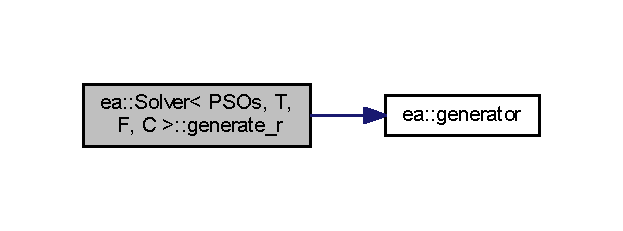
\includegraphics[width=299pt]{classea_1_1_solver_3_01_p_s_os_00_01_t_00_01_f_00_01_c_01_4_a01ea94eec2b6f05c62c9f83d725bb75b_cgraph}
\end{center}
\end{figure}
\mbox{\Hypertarget{classea_1_1_solver_3_01_p_s_os_00_01_t_00_01_f_00_01_c_01_4_a91feb28b5a3b292da8eedb1f782d53c0}\label{classea_1_1_solver_3_01_p_s_os_00_01_t_00_01_f_00_01_c_01_4_a91feb28b5a3b292da8eedb1f782d53c0}} 
\index{ea\+::\+Solver$<$ P\+S\+Os, T, F, C $>$@{ea\+::\+Solver$<$ P\+S\+Os, T, F, C $>$}!position\+\_\+update@{position\+\_\+update}}
\index{position\+\_\+update@{position\+\_\+update}!ea\+::\+Solver$<$ P\+S\+Os, T, F, C $>$@{ea\+::\+Solver$<$ P\+S\+Os, T, F, C $>$}}
\subsubsection{\texorpdfstring{position\+\_\+update()}{position\_update()}}
{\footnotesize\ttfamily template$<$typename T , typename F , typename C $>$ \\
void \hyperlink{classea_1_1_solver}{ea\+::\+Solver}$<$ \hyperlink{structea_1_1_p_s_os}{P\+S\+Os}, T, F, C $>$\+::position\+\_\+update (\begin{DoxyParamCaption}{ }\end{DoxyParamCaption})\hspace{0.3cm}{\ttfamily [private]}}



Position update of the particles. 

\begin{DoxyReturn}{Returns}
void 
\end{DoxyReturn}


Definition at line 248 of file pso\+\_\+sub\+\_\+swarm.\+h.



References ea\+::\+P\+S\+Os$<$ T $>$\+::vmax.


\begin{DoxyCode}
249     \{
250         \textcolor{keywordflow}{for} (\textcolor{keywordtype}{size\_t} i = 0; i < \hyperlink{classea_1_1_solver_3_01_p_s_os_00_01_t_00_01_f_00_01_c_01_4_a1f1aa62756a73565ebe0ca1fbc084ea5}{pso}.npop; ++i)
251         \{
252             \textcolor{keywordflow}{for} (\textcolor{keywordtype}{size\_t} j = 0; j < \hyperlink{classea_1_1_solver_3_01_p_s_os_00_01_t_00_01_f_00_01_c_01_4_a1f1aa62756a73565ebe0ca1fbc084ea5}{pso}.ndv; ++j)
253             \{
254                 \textcolor{keyword}{const} \textcolor{keyword}{auto}& r = \hyperlink{classea_1_1_solver_3_01_p_s_os_00_01_t_00_01_f_00_01_c_01_4_a01ea94eec2b6f05c62c9f83d725bb75b}{generate\_r}();
255                 \hyperlink{classea_1_1_solver_3_01_p_s_os_00_01_t_00_01_f_00_01_c_01_4_ac188af95a817ad70538969bd5af2dc66}{velocity}[i][j] = 0.729 * \hyperlink{classea_1_1_solver_3_01_p_s_os_00_01_t_00_01_f_00_01_c_01_4_ac188af95a817ad70538969bd5af2dc66}{velocity}[i][j] + \textcolor{comment}{//pso.c1 * r[0][j] *
       (personal\_best[i][j] - this->individuals[i][j])}
256                     + \hyperlink{classea_1_1_solver_3_01_p_s_os_00_01_t_00_01_f_00_01_c_01_4_a1f1aa62756a73565ebe0ca1fbc084ea5}{pso}.c2 * r[1][j] * (\hyperlink{classea_1_1_solver_3_01_p_s_os_00_01_t_00_01_f_00_01_c_01_4_afa2eb13f0e5028ba4aa96f7e29b62e9c}{local\_best}[\hyperlink{classea_1_1_solver_3_01_p_s_os_00_01_t_00_01_f_00_01_c_01_4_a192926bdbed79d0cd68867c4f695cd92}{neighbourhoods}[i]][j] - 
      this->\hyperlink{classea_1_1_solver__base_ad75bc440d24a46e97694c7c889f2ecde}{individuals}[i][j]) \textcolor{comment}{//+(w / 2) * r[2][j]*(min\_cost[j] - this->individuals[i][j]);}
257                     ;
258                 \textcolor{keywordflow}{if} (\hyperlink{classea_1_1_solver_3_01_p_s_os_00_01_t_00_01_f_00_01_c_01_4_ac188af95a817ad70538969bd5af2dc66}{velocity}[i][j] > \hyperlink{classea_1_1_solver_3_01_p_s_os_00_01_t_00_01_f_00_01_c_01_4_ade5fde673b93afeb9e3cb410d6f1061a}{vmax}[j])
259                 \{
260                     \hyperlink{classea_1_1_solver_3_01_p_s_os_00_01_t_00_01_f_00_01_c_01_4_ac188af95a817ad70538969bd5af2dc66}{velocity}[i][j] = \hyperlink{classea_1_1_solver_3_01_p_s_os_00_01_t_00_01_f_00_01_c_01_4_ade5fde673b93afeb9e3cb410d6f1061a}{vmax}[j];
261                 \}
262                 this->\hyperlink{classea_1_1_solver__base_ad75bc440d24a46e97694c7c889f2ecde}{individuals}[i][j] = this->\hyperlink{classea_1_1_solver__base_ad75bc440d24a46e97694c7c889f2ecde}{individuals}[i][j] + 
      \hyperlink{classea_1_1_solver_3_01_p_s_os_00_01_t_00_01_f_00_01_c_01_4_ac188af95a817ad70538969bd5af2dc66}{velocity}[i][j];
263             \}
264         \}
265     \}
\end{DoxyCode}
\mbox{\Hypertarget{classea_1_1_solver_3_01_p_s_os_00_01_t_00_01_f_00_01_c_01_4_a4952777e6e95820c9702e9306e24d1fb}\label{classea_1_1_solver_3_01_p_s_os_00_01_t_00_01_f_00_01_c_01_4_a4952777e6e95820c9702e9306e24d1fb}} 
\index{ea\+::\+Solver$<$ P\+S\+Os, T, F, C $>$@{ea\+::\+Solver$<$ P\+S\+Os, T, F, C $>$}!run\+\_\+algo@{run\+\_\+algo}}
\index{run\+\_\+algo@{run\+\_\+algo}!ea\+::\+Solver$<$ P\+S\+Os, T, F, C $>$@{ea\+::\+Solver$<$ P\+S\+Os, T, F, C $>$}}
\subsubsection{\texorpdfstring{run\+\_\+algo()}{run\_algo()}}
{\footnotesize\ttfamily template$<$typename T , typename F , typename C $>$ \\
void \hyperlink{classea_1_1_solver}{ea\+::\+Solver}$<$ \hyperlink{structea_1_1_p_s_os}{P\+S\+Os}, T, F, C $>$\+::run\+\_\+algo (\begin{DoxyParamCaption}{ }\end{DoxyParamCaption})\hspace{0.3cm}{\ttfamily [private]}}



Runs the algorithm until stopping criteria return void. 

Local Best Particle Swarm starts here

Inertia is updated 

Definition at line 334 of file pso\+\_\+sub\+\_\+swarm.\+h.



References ea\+::\+P\+S\+Os$<$ T $>$\+::w.


\begin{DoxyCode}
335     \{
337         \textcolor{keywordflow}{for} (\textcolor{keywordtype}{size\_t} iter = 0; iter < \hyperlink{classea_1_1_solver_3_01_p_s_os_00_01_t_00_01_f_00_01_c_01_4_a1f1aa62756a73565ebe0ca1fbc084ea5}{pso}.iter\_max; ++iter)
338         \{
339             \hyperlink{classea_1_1_solver_3_01_p_s_os_00_01_t_00_01_f_00_01_c_01_4_a91feb28b5a3b292da8eedb1f782d53c0}{position\_update}();
340             \hyperlink{classea_1_1_solver_3_01_p_s_os_00_01_t_00_01_f_00_01_c_01_4_ab52c41eb3bea4aa9465ff254bee82990}{best\_update}();
341             \hyperlink{classea_1_1_solver_3_01_p_s_os_00_01_t_00_01_f_00_01_c_01_4_a012b67607139916c790167fefc1f38e7}{find\_min\_local\_best}();
343             \hyperlink{classea_1_1_solver_3_01_p_s_os_00_01_t_00_01_f_00_01_c_01_4_a4f690e68bf36069ba446ef96b03da6f6}{w} = \hyperlink{classea_1_1_solver_3_01_p_s_os_00_01_t_00_01_f_00_01_c_01_4_a1f1aa62756a73565ebe0ca1fbc084ea5}{pso}.w - (\hyperlink{classea_1_1_solver_3_01_p_s_os_00_01_t_00_01_f_00_01_c_01_4_a1f1aa62756a73565ebe0ca1fbc084ea5}{pso}.w - 0.4) * std::pow((static\_cast<T>(iter) / static\_cast<T>(
      \hyperlink{classea_1_1_solver_3_01_p_s_os_00_01_t_00_01_f_00_01_c_01_4_a1f1aa62756a73565ebe0ca1fbc084ea5}{pso}.iter\_max)), inv\_pi\_sq\_2<T>);
344             this->\hyperlink{classea_1_1_solver__base_a8f9a321eb87e57636cf0b0f3a57b6fc2}{last\_iter} = iter;
345             \textcolor{keywordflow}{if} (\hyperlink{classea_1_1_solver_3_01_p_s_os_00_01_t_00_01_f_00_01_c_01_4_afd7a166bcdc0730431ca9406f0d0e030}{check\_pso\_criteria}())
346             \{
347                 this->\hyperlink{classea_1_1_solver__base_a1cdb824e8df6d4a8f228820ea85c9b05}{solved\_flag} = \textcolor{keyword}{true};
348                 \textcolor{keywordflow}{break};
349             \}
350         \}
351     \}
\end{DoxyCode}
\mbox{\Hypertarget{classea_1_1_solver_3_01_p_s_os_00_01_t_00_01_f_00_01_c_01_4_acf9a10b2f3e095c365fa787c06709a3d}\label{classea_1_1_solver_3_01_p_s_os_00_01_t_00_01_f_00_01_c_01_4_acf9a10b2f3e095c365fa787c06709a3d}} 
\index{ea\+::\+Solver$<$ P\+S\+Os, T, F, C $>$@{ea\+::\+Solver$<$ P\+S\+Os, T, F, C $>$}!set\+\_\+neighbourhoods@{set\+\_\+neighbourhoods}}
\index{set\+\_\+neighbourhoods@{set\+\_\+neighbourhoods}!ea\+::\+Solver$<$ P\+S\+Os, T, F, C $>$@{ea\+::\+Solver$<$ P\+S\+Os, T, F, C $>$}}
\subsubsection{\texorpdfstring{set\+\_\+neighbourhoods()}{set\_neighbourhoods()}}
{\footnotesize\ttfamily template$<$typename T , typename F , typename C $>$ \\
std\+::unordered\+\_\+map$<$ size\+\_\+t, size\+\_\+t $>$ \hyperlink{classea_1_1_solver}{ea\+::\+Solver}$<$ \hyperlink{structea_1_1_p_s_os}{P\+S\+Os}, T, F, C $>$\+::set\+\_\+neighbourhoods (\begin{DoxyParamCaption}{ }\end{DoxyParamCaption})\hspace{0.3cm}{\ttfamily [private]}}



Set the neighbourhoods of the algorithm using particle indices. 

\begin{DoxyReturn}{Returns}
A map matching particle indices to neighbourhoods 
\end{DoxyReturn}


Definition at line 212 of file pso\+\_\+sub\+\_\+swarm.\+h.


\begin{DoxyCode}
213     \{
214         std::unordered\_map<size\_t, size\_t> \hyperlink{classea_1_1_solver_3_01_p_s_os_00_01_t_00_01_f_00_01_c_01_4_a192926bdbed79d0cd68867c4f695cd92}{neighbourhoods};
215         \textcolor{keywordtype}{size\_t} neigh\_index = 0;
216         \textcolor{keywordtype}{size\_t} counter = 0;
217         \textcolor{keywordflow}{for} (\textcolor{keywordtype}{size\_t} i = 0; i < \hyperlink{classea_1_1_solver_3_01_p_s_os_00_01_t_00_01_f_00_01_c_01_4_a1f1aa62756a73565ebe0ca1fbc084ea5}{pso}.npop; ++i)
218         \{
219             \textcolor{keywordflow}{if} (counter < \hyperlink{classea_1_1_solver_3_01_p_s_os_00_01_t_00_01_f_00_01_c_01_4_a1f1aa62756a73565ebe0ca1fbc084ea5}{pso}.sneigh)
220             \{
221                 neighbourhoods[i] = neigh\_index;
222                 counter = counter + 1;
223             \}
224             \textcolor{keywordflow}{else}
225             \{
226                 neigh\_index = neigh\_index + 1;
227                 counter = 0;
228             \}
229         \}
230         \textcolor{keywordflow}{return} \hyperlink{classea_1_1_solver_3_01_p_s_os_00_01_t_00_01_f_00_01_c_01_4_a192926bdbed79d0cd68867c4f695cd92}{neighbourhoods};
231     \}
\end{DoxyCode}


\subsection{Friends And Related Function Documentation}
\mbox{\Hypertarget{classea_1_1_solver_3_01_p_s_os_00_01_t_00_01_f_00_01_c_01_4_aa3dcae3fc6bad98284e958b7c320549c}\label{classea_1_1_solver_3_01_p_s_os_00_01_t_00_01_f_00_01_c_01_4_aa3dcae3fc6bad98284e958b7c320549c}} 
\index{ea\+::\+Solver$<$ P\+S\+Os, T, F, C $>$@{ea\+::\+Solver$<$ P\+S\+Os, T, F, C $>$}!Solver\+\_\+base$<$ Solver$<$ P\+S\+Os, T, F, C $>$, P\+S\+Os, T, F, C $>$@{Solver\+\_\+base$<$ Solver$<$ P\+S\+Os, T, F, C $>$, P\+S\+Os, T, F, C $>$}}
\index{Solver\+\_\+base$<$ Solver$<$ P\+S\+Os, T, F, C $>$, P\+S\+Os, T, F, C $>$@{Solver\+\_\+base$<$ Solver$<$ P\+S\+Os, T, F, C $>$, P\+S\+Os, T, F, C $>$}!ea\+::\+Solver$<$ P\+S\+Os, T, F, C $>$@{ea\+::\+Solver$<$ P\+S\+Os, T, F, C $>$}}
\subsubsection{\texorpdfstring{Solver\+\_\+base$<$ Solver$<$ P\+S\+Os, T, F, C $>$, P\+S\+Os, T, F, C $>$}{Solver\_base< Solver< PSOs, T, F, C >, PSOs, T, F, C >}}
{\footnotesize\ttfamily template$<$typename T , typename F , typename C $>$ \\
friend class \hyperlink{classea_1_1_solver__base}{Solver\+\_\+base}$<$ \hyperlink{classea_1_1_solver}{Solver}$<$ \hyperlink{structea_1_1_p_s_os}{P\+S\+Os}, T, F, C $>$, \hyperlink{structea_1_1_p_s_os}{P\+S\+Os}, T, F, C $>$\hspace{0.3cm}{\ttfamily [friend]}}



Definition at line 86 of file pso\+\_\+sub\+\_\+swarm.\+h.



\subsection{Member Data Documentation}
\mbox{\Hypertarget{classea_1_1_solver_3_01_p_s_os_00_01_t_00_01_f_00_01_c_01_4_afa2eb13f0e5028ba4aa96f7e29b62e9c}\label{classea_1_1_solver_3_01_p_s_os_00_01_t_00_01_f_00_01_c_01_4_afa2eb13f0e5028ba4aa96f7e29b62e9c}} 
\index{ea\+::\+Solver$<$ P\+S\+Os, T, F, C $>$@{ea\+::\+Solver$<$ P\+S\+Os, T, F, C $>$}!local\+\_\+best@{local\+\_\+best}}
\index{local\+\_\+best@{local\+\_\+best}!ea\+::\+Solver$<$ P\+S\+Os, T, F, C $>$@{ea\+::\+Solver$<$ P\+S\+Os, T, F, C $>$}}
\subsubsection{\texorpdfstring{local\+\_\+best}{local\_best}}
{\footnotesize\ttfamily template$<$typename T , typename F , typename C $>$ \\
std\+::vector$<$std\+::vector$<$T$>$ $>$ \hyperlink{classea_1_1_solver}{ea\+::\+Solver}$<$ \hyperlink{structea_1_1_p_s_os}{P\+S\+Os}, T, F, C $>$\+::local\+\_\+best\hspace{0.3cm}{\ttfamily [private]}}



Local best vector, holds the best position recorded for each neighbourhood. 



Definition at line 138 of file pso\+\_\+sub\+\_\+swarm.\+h.

\mbox{\Hypertarget{classea_1_1_solver_3_01_p_s_os_00_01_t_00_01_f_00_01_c_01_4_a192926bdbed79d0cd68867c4f695cd92}\label{classea_1_1_solver_3_01_p_s_os_00_01_t_00_01_f_00_01_c_01_4_a192926bdbed79d0cd68867c4f695cd92}} 
\index{ea\+::\+Solver$<$ P\+S\+Os, T, F, C $>$@{ea\+::\+Solver$<$ P\+S\+Os, T, F, C $>$}!neighbourhoods@{neighbourhoods}}
\index{neighbourhoods@{neighbourhoods}!ea\+::\+Solver$<$ P\+S\+Os, T, F, C $>$@{ea\+::\+Solver$<$ P\+S\+Os, T, F, C $>$}}
\subsubsection{\texorpdfstring{neighbourhoods}{neighbourhoods}}
{\footnotesize\ttfamily template$<$typename T , typename F , typename C $>$ \\
std\+::unordered\+\_\+map$<$size\+\_\+t, size\+\_\+t$>$ \hyperlink{classea_1_1_solver}{ea\+::\+Solver}$<$ \hyperlink{structea_1_1_p_s_os}{P\+S\+Os}, T, F, C $>$\+::neighbourhoods\hspace{0.3cm}{\ttfamily [private]}}



Neighbourhoods. 



Definition at line 144 of file pso\+\_\+sub\+\_\+swarm.\+h.

\mbox{\Hypertarget{classea_1_1_solver_3_01_p_s_os_00_01_t_00_01_f_00_01_c_01_4_a92980b9d3411dd8855a6a050722ebcf7}\label{classea_1_1_solver_3_01_p_s_os_00_01_t_00_01_f_00_01_c_01_4_a92980b9d3411dd8855a6a050722ebcf7}} 
\index{ea\+::\+Solver$<$ P\+S\+Os, T, F, C $>$@{ea\+::\+Solver$<$ P\+S\+Os, T, F, C $>$}!nneigh@{nneigh}}
\index{nneigh@{nneigh}!ea\+::\+Solver$<$ P\+S\+Os, T, F, C $>$@{ea\+::\+Solver$<$ P\+S\+Os, T, F, C $>$}}
\subsubsection{\texorpdfstring{nneigh}{nneigh}}
{\footnotesize\ttfamily template$<$typename T , typename F , typename C $>$ \\
const size\+\_\+t \hyperlink{classea_1_1_solver}{ea\+::\+Solver}$<$ \hyperlink{structea_1_1_p_s_os}{P\+S\+Os}, T, F, C $>$\+::nneigh\hspace{0.3cm}{\ttfamily [private]}}



Number of neighbourhoods. 



Definition at line 142 of file pso\+\_\+sub\+\_\+swarm.\+h.

\mbox{\Hypertarget{classea_1_1_solver_3_01_p_s_os_00_01_t_00_01_f_00_01_c_01_4_a8a857e38363bd1ed23ea77e262b9b710}\label{classea_1_1_solver_3_01_p_s_os_00_01_t_00_01_f_00_01_c_01_4_a8a857e38363bd1ed23ea77e262b9b710}} 
\index{ea\+::\+Solver$<$ P\+S\+Os, T, F, C $>$@{ea\+::\+Solver$<$ P\+S\+Os, T, F, C $>$}!personal\+\_\+best@{personal\+\_\+best}}
\index{personal\+\_\+best@{personal\+\_\+best}!ea\+::\+Solver$<$ P\+S\+Os, T, F, C $>$@{ea\+::\+Solver$<$ P\+S\+Os, T, F, C $>$}}
\subsubsection{\texorpdfstring{personal\+\_\+best}{personal\_best}}
{\footnotesize\ttfamily template$<$typename T , typename F , typename C $>$ \\
std\+::vector$<$std\+::vector$<$T$>$ $>$ \hyperlink{classea_1_1_solver}{ea\+::\+Solver}$<$ \hyperlink{structea_1_1_p_s_os}{P\+S\+Os}, T, F, C $>$\+::personal\+\_\+best\hspace{0.3cm}{\ttfamily [private]}}



Personal best vector of the particles, holds the best position recorded for each particle. 



Definition at line 136 of file pso\+\_\+sub\+\_\+swarm.\+h.

\mbox{\Hypertarget{classea_1_1_solver_3_01_p_s_os_00_01_t_00_01_f_00_01_c_01_4_a1f1aa62756a73565ebe0ca1fbc084ea5}\label{classea_1_1_solver_3_01_p_s_os_00_01_t_00_01_f_00_01_c_01_4_a1f1aa62756a73565ebe0ca1fbc084ea5}} 
\index{ea\+::\+Solver$<$ P\+S\+Os, T, F, C $>$@{ea\+::\+Solver$<$ P\+S\+Os, T, F, C $>$}!pso@{pso}}
\index{pso@{pso}!ea\+::\+Solver$<$ P\+S\+Os, T, F, C $>$@{ea\+::\+Solver$<$ P\+S\+Os, T, F, C $>$}}
\subsubsection{\texorpdfstring{pso}{pso}}
{\footnotesize\ttfamily template$<$typename T , typename F , typename C $>$ \\
const \hyperlink{structea_1_1_p_s_os}{P\+S\+Os}$<$T$>$\& \hyperlink{classea_1_1_solver}{ea\+::\+Solver}$<$ \hyperlink{structea_1_1_p_s_os}{P\+S\+Os}, T, F, C $>$\+::pso\hspace{0.3cm}{\ttfamily [private]}}



Particle Swarm Optimisation structure used internally (reference to solver\+\_\+struct) 



Definition at line 130 of file pso\+\_\+sub\+\_\+swarm.\+h.

\mbox{\Hypertarget{classea_1_1_solver_3_01_p_s_os_00_01_t_00_01_f_00_01_c_01_4_ac188af95a817ad70538969bd5af2dc66}\label{classea_1_1_solver_3_01_p_s_os_00_01_t_00_01_f_00_01_c_01_4_ac188af95a817ad70538969bd5af2dc66}} 
\index{ea\+::\+Solver$<$ P\+S\+Os, T, F, C $>$@{ea\+::\+Solver$<$ P\+S\+Os, T, F, C $>$}!velocity@{velocity}}
\index{velocity@{velocity}!ea\+::\+Solver$<$ P\+S\+Os, T, F, C $>$@{ea\+::\+Solver$<$ P\+S\+Os, T, F, C $>$}}
\subsubsection{\texorpdfstring{velocity}{velocity}}
{\footnotesize\ttfamily template$<$typename T , typename F , typename C $>$ \\
std\+::vector$<$std\+::vector$<$T$>$ $>$ \hyperlink{classea_1_1_solver}{ea\+::\+Solver}$<$ \hyperlink{structea_1_1_p_s_os}{P\+S\+Os}, T, F, C $>$\+::velocity\hspace{0.3cm}{\ttfamily [private]}}



Velocity of the particles. 



Definition at line 140 of file pso\+\_\+sub\+\_\+swarm.\+h.

\mbox{\Hypertarget{classea_1_1_solver_3_01_p_s_os_00_01_t_00_01_f_00_01_c_01_4_ade5fde673b93afeb9e3cb410d6f1061a}\label{classea_1_1_solver_3_01_p_s_os_00_01_t_00_01_f_00_01_c_01_4_ade5fde673b93afeb9e3cb410d6f1061a}} 
\index{ea\+::\+Solver$<$ P\+S\+Os, T, F, C $>$@{ea\+::\+Solver$<$ P\+S\+Os, T, F, C $>$}!vmax@{vmax}}
\index{vmax@{vmax}!ea\+::\+Solver$<$ P\+S\+Os, T, F, C $>$@{ea\+::\+Solver$<$ P\+S\+Os, T, F, C $>$}}
\subsubsection{\texorpdfstring{vmax}{vmax}}
{\footnotesize\ttfamily template$<$typename T , typename F , typename C $>$ \\
std\+::vector$<$T$>$ \hyperlink{classea_1_1_solver}{ea\+::\+Solver}$<$ \hyperlink{structea_1_1_p_s_os}{P\+S\+Os}, T, F, C $>$\+::vmax\hspace{0.3cm}{\ttfamily [private]}}



Maximum Velocity is mutable, so a copy is created. 



Definition at line 134 of file pso\+\_\+sub\+\_\+swarm.\+h.

\mbox{\Hypertarget{classea_1_1_solver_3_01_p_s_os_00_01_t_00_01_f_00_01_c_01_4_a4f690e68bf36069ba446ef96b03da6f6}\label{classea_1_1_solver_3_01_p_s_os_00_01_t_00_01_f_00_01_c_01_4_a4f690e68bf36069ba446ef96b03da6f6}} 
\index{ea\+::\+Solver$<$ P\+S\+Os, T, F, C $>$@{ea\+::\+Solver$<$ P\+S\+Os, T, F, C $>$}!w@{w}}
\index{w@{w}!ea\+::\+Solver$<$ P\+S\+Os, T, F, C $>$@{ea\+::\+Solver$<$ P\+S\+Os, T, F, C $>$}}
\subsubsection{\texorpdfstring{w}{w}}
{\footnotesize\ttfamily template$<$typename T , typename F , typename C $>$ \\
T \hyperlink{classea_1_1_solver}{ea\+::\+Solver}$<$ \hyperlink{structea_1_1_p_s_os}{P\+S\+Os}, T, F, C $>$\+::w\hspace{0.3cm}{\ttfamily [private]}}



Inertia is mutable, so a copy is created. 



Definition at line 132 of file pso\+\_\+sub\+\_\+swarm.\+h.



The documentation for this class was generated from the following file\+:\begin{DoxyCompactItemize}
\item 
\hyperlink{pso__sub__swarm_8h}{pso\+\_\+sub\+\_\+swarm.\+h}\end{DoxyCompactItemize}

\hypertarget{classea_1_1_solver__base}{}\section{ea\+:\+:Solver\+\_\+base$<$ Derived, S, T, F, C $>$ Class Template Reference}
\label{classea_1_1_solver__base}\index{ea\+::\+Solver\+\_\+base$<$ Derived, S, T, F, C $>$@{ea\+::\+Solver\+\_\+base$<$ Derived, S, T, F, C $>$}}


Base Class for Evolutionary Algorithms.  




{\ttfamily \#include $<$ealgorithm\+\_\+base.\+h$>$}

\subsection*{Public Member Functions}
\begin{DoxyCompactItemize}
\item 
std\+::vector$<$ T $>$ \hyperlink{classea_1_1_solver__base_aa5cf33a16448e3a0ea3ddb61a3573fb0}{solver\+\_\+bench} (const std\+::string \&problem\+\_\+name)
\begin{DoxyCompactList}\small\item\em Solve wrapper function for Solvers, used for benchmarks. \end{DoxyCompactList}\end{DoxyCompactItemize}
\subsection*{Protected Member Functions}
\begin{DoxyCompactItemize}
\item 
\hyperlink{classea_1_1_solver__base_a3d0f28385218d7d869f3217adddcf93f}{Solver\+\_\+base} (const S$<$ T $>$ \&i\+\_\+solver\+\_\+struct, const F \&i\+\_\+f, const C \&i\+\_\+c)
\begin{DoxyCompactList}\small\item\em Constructor. \end{DoxyCompactList}\item 
std\+::vector$<$ T $>$ \hyperlink{classea_1_1_solver__base_a865cea7e218b633b440b88fa09e48466}{randomise\+\_\+individual} ()
\begin{DoxyCompactList}\small\item\em Returns a randomised individual using the initial decision variables and standard deviation. \end{DoxyCompactList}\item 
std\+::vector$<$ std\+::vector$<$ T $>$ $>$ \hyperlink{classea_1_1_solver__base_a3220df901d0e61d3c49e6265640d94ae}{init\+\_\+individuals} ()
\begin{DoxyCompactList}\small\item\em Initialises the population by randomising aroung the decision variables using the given standard deviation. \end{DoxyCompactList}\item 
void \hyperlink{classea_1_1_solver__base_ac69a6c714298054039acbbbf5d2eea23}{find\+\_\+min\+\_\+cost} ()
\begin{DoxyCompactList}\small\item\em Find the minimum cost individual of the fitness function for the population. \end{DoxyCompactList}\item 
std\+::stringstream \hyperlink{classea_1_1_solver__base_ae16049f3e8586c144165fa2916ccdbce}{display\+\_\+results} ()
\begin{DoxyCompactList}\small\item\em Display the results of execution of an algorithm as well as its parameters. \end{DoxyCompactList}\item 
void \hyperlink{classea_1_1_solver__base_a20dd7b75350cd42e13ecdc6c5714010a}{write\+\_\+results\+\_\+to\+\_\+file} (const std\+::string \&problem\+\_\+name)
\begin{DoxyCompactList}\small\item\em Write the results to a file. \end{DoxyCompactList}\end{DoxyCompactItemize}
\subsection*{Protected Attributes}
\begin{DoxyCompactItemize}
\item 
const S$<$ T $>$ \hyperlink{classea_1_1_solver__base_a5e1d821809f2d26c6f882942ad728127}{solver\+\_\+struct}
\begin{DoxyCompactList}\small\item\em Internal copy of the structure used for parameters of the algorithm. \end{DoxyCompactList}\item 
F \hyperlink{classea_1_1_solver__base_ae0a893780c93dfe17c1d17301de6494f}{f}
\begin{DoxyCompactList}\small\item\em Copy of the fitness function passed as a lambda. \end{DoxyCompactList}\item 
C \hyperlink{classea_1_1_solver__base_a6914e89d30e7484f2b4af1783f0de8c3}{c}
\begin{DoxyCompactList}\small\item\em Copy of the constraints function passed as a lambda. \end{DoxyCompactList}\item 
std\+::vector$<$ std\+::vector$<$ T $>$ $>$ \hyperlink{classea_1_1_solver__base_ad75bc440d24a46e97694c7c889f2ecde}{individuals}
\begin{DoxyCompactList}\small\item\em Population. \end{DoxyCompactList}\item 
std\+::vector$<$ T $>$ \hyperlink{classea_1_1_solver__base_af745cded954be26280d842c1e7c7f989}{min\+\_\+cost}
\begin{DoxyCompactList}\small\item\em Best solution / lowest fitness. \end{DoxyCompactList}\item 
size\+\_\+t \hyperlink{classea_1_1_solver__base_a8f9a321eb87e57636cf0b0f3a57b6fc2}{last\+\_\+iter}
\begin{DoxyCompactList}\small\item\em Last iteration to solution. \end{DoxyCompactList}\item 
bool \hyperlink{classea_1_1_solver__base_a1cdb824e8df6d4a8f228820ea85c9b05}{solved\+\_\+flag}
\begin{DoxyCompactList}\small\item\em A flag which determines if the solver has already solved the problem. \end{DoxyCompactList}\item 
T \hyperlink{classea_1_1_solver__base_ab0f0690de4b612c20b40f1b69a0e2743}{timer}
\begin{DoxyCompactList}\small\item\em The timer used for benchmarks. \end{DoxyCompactList}\item 
std\+::uniform\+\_\+real\+\_\+distribution$<$ T $>$ \hyperlink{classea_1_1_solver__base_ae88f44b13e264e092d3bbaeca6b3bd19}{distribution}
\begin{DoxyCompactList}\small\item\em Uniform real distribution. \end{DoxyCompactList}\end{DoxyCompactItemize}


\subsection{Detailed Description}
\subsubsection*{template$<$typename Derived, template$<$ typename $>$ class S, typename T, typename F, typename C$>$\newline
class ea\+::\+Solver\+\_\+base$<$ Derived, S, T, F, C $>$}

Base Class for Evolutionary Algorithms. 

The fitness and constraints functions are copied so that even if they are not available in the current scope, the solver will still execute properly. At the same time, std\+::function could be have used, thus eliminating the need for template parameters F and C. However, that comes at a runtime cost, since calls to the functions would be virtual and there is a possibility that allocation could happen on the heap. 

Definition at line 103 of file ealgorithm\+\_\+base.\+h.



\subsection{Constructor \& Destructor Documentation}
\mbox{\Hypertarget{classea_1_1_solver__base_a3d0f28385218d7d869f3217adddcf93f}\label{classea_1_1_solver__base_a3d0f28385218d7d869f3217adddcf93f}} 
\index{ea\+::\+Solver\+\_\+base@{ea\+::\+Solver\+\_\+base}!Solver\+\_\+base@{Solver\+\_\+base}}
\index{Solver\+\_\+base@{Solver\+\_\+base}!ea\+::\+Solver\+\_\+base@{ea\+::\+Solver\+\_\+base}}
\subsubsection{\texorpdfstring{Solver\+\_\+base()}{Solver\_base()}}
{\footnotesize\ttfamily template$<$typename Derived, template$<$ typename $>$ class S, typename T, typename F, typename C$>$ \\
\hyperlink{classea_1_1_solver__base}{ea\+::\+Solver\+\_\+base}$<$ Derived, S, T, F, C $>$\+::\hyperlink{classea_1_1_solver__base}{Solver\+\_\+base} (\begin{DoxyParamCaption}\item[{const S$<$ T $>$ \&}]{i\+\_\+solver\+\_\+struct,  }\item[{const F \&}]{i\+\_\+f,  }\item[{const C \&}]{i\+\_\+c }\end{DoxyParamCaption})\hspace{0.3cm}{\ttfamily [inline]}, {\ttfamily [protected]}}



Constructor. 


\begin{DoxyParams}{Parameters}
{\em i\+\_\+solver\+\_\+struct} & The parameter structure that is used to construct the solver \\
\hline
{\em i\+\_\+f} & A reference to the objective function \\
\hline
{\em i\+\_\+c} & A reference to the constraints function \\
\hline
\end{DoxyParams}
\begin{DoxyReturn}{Returns}
A Solver\+\_\+base$<$\+Derived, S, T, F, C$>$ object 
\end{DoxyReturn}


Definition at line 120 of file ealgorithm\+\_\+base.\+h.


\begin{DoxyCode}
120                                                                              :
121             \hyperlink{classea_1_1_solver__base_a5e1d821809f2d26c6f882942ad728127}{solver\_struct}\{ i\_solver\_struct \},
122             \hyperlink{classea_1_1_solver__base_ae0a893780c93dfe17c1d17301de6494f}{f}\{ i\_f \},
123             \hyperlink{classea_1_1_solver__base_a6914e89d30e7484f2b4af1783f0de8c3}{c}\{ i\_c \},
124             \hyperlink{classea_1_1_solver__base_ad75bc440d24a46e97694c7c889f2ecde}{individuals}\{ \hyperlink{classea_1_1_solver__base_a3220df901d0e61d3c49e6265640d94ae}{init\_individuals}() \},
125             \hyperlink{classea_1_1_solver__base_af745cded954be26280d842c1e7c7f989}{min\_cost}\{ \hyperlink{classea_1_1_solver__base_ad75bc440d24a46e97694c7c889f2ecde}{individuals}[0] \},
126             \hyperlink{classea_1_1_solver__base_a8f9a321eb87e57636cf0b0f3a57b6fc2}{last\_iter}\{ 0 \},
127             \hyperlink{classea_1_1_solver__base_a1cdb824e8df6d4a8f228820ea85c9b05}{solved\_flag}\{ \textcolor{keyword}{false} \},
128             \hyperlink{classea_1_1_solver__base_ab0f0690de4b612c20b40f1b69a0e2743}{timer}\{ 0 \},
129             \hyperlink{classea_1_1_solver__base_ae88f44b13e264e092d3bbaeca6b3bd19}{distribution}\{ std::uniform\_real\_distribution<T>(0.0, 1.0) \}
130         \{
131             \hyperlink{namespaceea_a385e8ca8ba4ae2f69dcfffa79f20c2ff}{generator}.discard(700000);
132             \hyperlink{classea_1_1_solver__base_ac69a6c714298054039acbbbf5d2eea23}{find\_min\_cost}();
133         \}
\end{DoxyCode}


\subsection{Member Function Documentation}
\mbox{\Hypertarget{classea_1_1_solver__base_ae16049f3e8586c144165fa2916ccdbce}\label{classea_1_1_solver__base_ae16049f3e8586c144165fa2916ccdbce}} 
\index{ea\+::\+Solver\+\_\+base@{ea\+::\+Solver\+\_\+base}!display\+\_\+results@{display\+\_\+results}}
\index{display\+\_\+results@{display\+\_\+results}!ea\+::\+Solver\+\_\+base@{ea\+::\+Solver\+\_\+base}}
\subsubsection{\texorpdfstring{display\+\_\+results()}{display\_results()}}
{\footnotesize\ttfamily template$<$typename Derived , template$<$ typename $>$ class S, typename T , typename F , typename C $>$ \\
std\+::stringstream \hyperlink{classea_1_1_solver__base}{ea\+::\+Solver\+\_\+base}$<$ Derived, S, T, F, C $>$\+::display\+\_\+results (\begin{DoxyParamCaption}{ }\end{DoxyParamCaption})\hspace{0.3cm}{\ttfamily [protected]}}



Display the results of execution of an algorithm as well as its parameters. 

\begin{DoxyReturn}{Returns}
A std\+::stringstream of the results 
\end{DoxyReturn}


Definition at line 223 of file ealgorithm\+\_\+base.\+h.


\begin{DoxyCode}
224     \{
225         std::stringstream results;
226         results << \textcolor{stringliteral}{"Algorithm:"} << \textcolor{stringliteral}{","} << \hyperlink{classea_1_1_solver__base_a5e1d821809f2d26c6f882942ad728127}{solver\_struct}.type << \textcolor{stringliteral}{","} << \textcolor{stringliteral}{"Solved:"} << \textcolor{stringliteral}{","};
227         \textcolor{keywordflow}{if} (!\hyperlink{classea_1_1_solver__base_a1cdb824e8df6d4a8f228820ea85c9b05}{solved\_flag})
228         \{
229             results << \textcolor{stringliteral}{"False"} << \textcolor{stringliteral}{","};
230         \}
231         \textcolor{keywordflow}{else}
232         \{
233             results << \textcolor{stringliteral}{"True"} << \textcolor{stringliteral}{","};
234         \}
235         results << \textcolor{stringliteral}{"Solution:"} << \textcolor{stringliteral}{","} <<  \hyperlink{classea_1_1_solver__base_af745cded954be26280d842c1e7c7f989}{min\_cost} << \textcolor{stringliteral}{","};
236         results << \textcolor{stringliteral}{"Fitness:"} << \textcolor{stringliteral}{","} << \hyperlink{classea_1_1_solver__base_ae0a893780c93dfe17c1d17301de6494f}{f}(min\_cost) << \textcolor{stringliteral}{","};
237         results << \textcolor{stringliteral}{"Population:"} << \textcolor{stringliteral}{","} << \hyperlink{classea_1_1_solver__base_ad75bc440d24a46e97694c7c889f2ecde}{individuals}.size() << \textcolor{stringliteral}{","};
238         results << \textcolor{stringliteral}{"Iterations:"} << \textcolor{stringliteral}{","} << \hyperlink{classea_1_1_solver__base_a8f9a321eb87e57636cf0b0f3a57b6fc2}{last\_iter} << \textcolor{stringliteral}{","};
239         results << \textcolor{stringliteral}{"Elapsed Time:"} << \textcolor{stringliteral}{","} << \hyperlink{classea_1_1_solver__base_ab0f0690de4b612c20b40f1b69a0e2743}{timer} << \textcolor{stringliteral}{","};
240         results << \textcolor{stringliteral}{"Starting Values:"} << \textcolor{stringliteral}{","} << \hyperlink{classea_1_1_solver__base_a5e1d821809f2d26c6f882942ad728127}{solver\_struct}.decision\_variables << \textcolor{stringliteral}{","};
241         results << \textcolor{stringliteral}{"Standard Deviation:"} << \textcolor{stringliteral}{","} << \hyperlink{classea_1_1_solver__base_a5e1d821809f2d26c6f882942ad728127}{solver\_struct}.stdev << \textcolor{stringliteral}{","};
242         results << \textcolor{stringliteral}{"Initial Population:"} << \textcolor{stringliteral}{","} << \hyperlink{classea_1_1_solver__base_a5e1d821809f2d26c6f882942ad728127}{solver\_struct}.npop << \textcolor{stringliteral}{","};
243         results << \textcolor{stringliteral}{"Tolerance:"} << \textcolor{stringliteral}{","} << \hyperlink{classea_1_1_solver__base_a5e1d821809f2d26c6f882942ad728127}{solver\_struct}.tol << \textcolor{stringliteral}{","};
244         results << \textcolor{stringliteral}{"Maximum Iterations:"} << \textcolor{stringliteral}{","} << \hyperlink{classea_1_1_solver__base_a5e1d821809f2d26c6f882942ad728127}{solver\_struct}.iter\_max << \textcolor{stringliteral}{","};
245         results << \textcolor{stringliteral}{"Using Penalty Function:"} << \textcolor{stringliteral}{","} << \hyperlink{classea_1_1_solver__base_a5e1d821809f2d26c6f882942ad728127}{solver\_struct}.use\_penalty\_method << \textcolor{stringliteral}{","}
      ;
246         results << \textcolor{stringliteral}{"Using Constraints:"} << \textcolor{stringliteral}{","};
247         \textcolor{keywordflow}{switch} (\hyperlink{classea_1_1_solver__base_a5e1d821809f2d26c6f882942ad728127}{solver\_struct}.constraints\_type)
248         \{
249         \textcolor{keywordflow}{case}(Constraints\_type::normal): results << \textcolor{stringliteral}{"Normal"} << \textcolor{stringliteral}{","}; \textcolor{keywordflow}{break};
250         \textcolor{keywordflow}{case}(Constraints\_type::tight): results << \textcolor{stringliteral}{"Tight"} << \textcolor{stringliteral}{","}; \textcolor{keywordflow}{break};
251         \textcolor{keywordflow}{case}(\hyperlink{namespaceea_a8e369877773b4db67b8512efdb4f8f89a334c4a4c42fdb79d7ebc3e73b517e6f8}{Constraints\_type::none}): results << \textcolor{stringliteral}{"None"} << \textcolor{stringliteral}{","}; \textcolor{keywordflow}{break};
252         \}
253         results << static\_cast<Derived*>(\textcolor{keyword}{this})->display\_parameters().str() << \textcolor{stringliteral}{"\(\backslash\)n"};
254         \textcolor{keywordflow}{return} results;
255     \}
\end{DoxyCode}
\mbox{\Hypertarget{classea_1_1_solver__base_ac69a6c714298054039acbbbf5d2eea23}\label{classea_1_1_solver__base_ac69a6c714298054039acbbbf5d2eea23}} 
\index{ea\+::\+Solver\+\_\+base@{ea\+::\+Solver\+\_\+base}!find\+\_\+min\+\_\+cost@{find\+\_\+min\+\_\+cost}}
\index{find\+\_\+min\+\_\+cost@{find\+\_\+min\+\_\+cost}!ea\+::\+Solver\+\_\+base@{ea\+::\+Solver\+\_\+base}}
\subsubsection{\texorpdfstring{find\+\_\+min\+\_\+cost()}{find\_min\_cost()}}
{\footnotesize\ttfamily template$<$typename Derived , template$<$ typename $>$ class S, typename T , typename F , typename C $>$ \\
void \hyperlink{classea_1_1_solver__base}{ea\+::\+Solver\+\_\+base}$<$ Derived, S, T, F, C $>$\+::find\+\_\+min\+\_\+cost (\begin{DoxyParamCaption}{ }\end{DoxyParamCaption})\hspace{0.3cm}{\ttfamily [protected]}}



Find the minimum cost individual of the fitness function for the population. 

\begin{DoxyReturn}{Returns}
void 
\end{DoxyReturn}


Definition at line 211 of file ealgorithm\+\_\+base.\+h.


\begin{DoxyCode}
212     \{
213         \textcolor{keywordflow}{for} (\textcolor{keyword}{const} \textcolor{keyword}{auto}& p : \hyperlink{classea_1_1_solver__base_ad75bc440d24a46e97694c7c889f2ecde}{individuals})
214         \{
215             \textcolor{keywordflow}{if} (\hyperlink{classea_1_1_solver__base_ae0a893780c93dfe17c1d17301de6494f}{f}(\hyperlink{classea_1_1_solver__base_af745cded954be26280d842c1e7c7f989}{min\_cost}) > \hyperlink{classea_1_1_solver__base_ae0a893780c93dfe17c1d17301de6494f}{f}(p))
216             \{
217                 \hyperlink{classea_1_1_solver__base_af745cded954be26280d842c1e7c7f989}{min\_cost} = p;
218             \}
219         \}
220     \}
\end{DoxyCode}
\mbox{\Hypertarget{classea_1_1_solver__base_a3220df901d0e61d3c49e6265640d94ae}\label{classea_1_1_solver__base_a3220df901d0e61d3c49e6265640d94ae}} 
\index{ea\+::\+Solver\+\_\+base@{ea\+::\+Solver\+\_\+base}!init\+\_\+individuals@{init\+\_\+individuals}}
\index{init\+\_\+individuals@{init\+\_\+individuals}!ea\+::\+Solver\+\_\+base@{ea\+::\+Solver\+\_\+base}}
\subsubsection{\texorpdfstring{init\+\_\+individuals()}{init\_individuals()}}
{\footnotesize\ttfamily template$<$typename Derived , template$<$ typename $>$ class S, typename T , typename F , typename C $>$ \\
std\+::vector$<$ std\+::vector$<$ T $>$ $>$ \hyperlink{classea_1_1_solver__base}{ea\+::\+Solver\+\_\+base}$<$ Derived, S, T, F, C $>$\+::init\+\_\+individuals (\begin{DoxyParamCaption}{ }\end{DoxyParamCaption})\hspace{0.3cm}{\ttfamily [protected]}}



Initialises the population by randomising aroung the decision variables using the given standard deviation. 

\begin{DoxyReturn}{Returns}
The population after checking the constraints of the optimisation problem 
\end{DoxyReturn}
Check population constraints 

Definition at line 195 of file ealgorithm\+\_\+base.\+h.


\begin{DoxyCode}
196     \{
197         std::vector<std::vector<T>> \hyperlink{classea_1_1_solver__base_ad75bc440d24a46e97694c7c889f2ecde}{individuals}(\hyperlink{classea_1_1_solver__base_a5e1d821809f2d26c6f882942ad728127}{solver\_struct}.npop, std::vector<T>(
      \hyperlink{classea_1_1_solver__base_a5e1d821809f2d26c6f882942ad728127}{solver\_struct}.ndv));
198         \textcolor{keywordflow}{for} (\textcolor{keyword}{auto}& p : \hyperlink{classea_1_1_solver__base_ad75bc440d24a46e97694c7c889f2ecde}{individuals})
199         \{
200             p = \hyperlink{classea_1_1_solver__base_a865cea7e218b633b440b88fa09e48466}{randomise\_individual}();
202             \textcolor{keywordflow}{while} (!\hyperlink{classea_1_1_solver__base_a6914e89d30e7484f2b4af1783f0de8c3}{c}(p))
203             \{
204                 p = \hyperlink{classea_1_1_solver__base_a865cea7e218b633b440b88fa09e48466}{randomise\_individual}();
205             \}
206         \}
207         \textcolor{keywordflow}{return} \hyperlink{classea_1_1_solver__base_ad75bc440d24a46e97694c7c889f2ecde}{individuals};
208     \}
\end{DoxyCode}
\mbox{\Hypertarget{classea_1_1_solver__base_a865cea7e218b633b440b88fa09e48466}\label{classea_1_1_solver__base_a865cea7e218b633b440b88fa09e48466}} 
\index{ea\+::\+Solver\+\_\+base@{ea\+::\+Solver\+\_\+base}!randomise\+\_\+individual@{randomise\+\_\+individual}}
\index{randomise\+\_\+individual@{randomise\+\_\+individual}!ea\+::\+Solver\+\_\+base@{ea\+::\+Solver\+\_\+base}}
\subsubsection{\texorpdfstring{randomise\+\_\+individual()}{randomise\_individual()}}
{\footnotesize\ttfamily template$<$typename Derived , template$<$ typename $>$ class S, typename T , typename F , typename C $>$ \\
std\+::vector$<$ T $>$ \hyperlink{classea_1_1_solver__base}{ea\+::\+Solver\+\_\+base}$<$ Derived, S, T, F, C $>$\+::randomise\+\_\+individual (\begin{DoxyParamCaption}{ }\end{DoxyParamCaption})\hspace{0.3cm}{\ttfamily [protected]}}



Returns a randomised individual using the initial decision variables and standard deviation. 

\begin{DoxyReturn}{Returns}
A randomised individual of type std\+::vector$<$\+T$>$, where T is a floating-\/point number type. 
\end{DoxyReturn}


Definition at line 181 of file ealgorithm\+\_\+base.\+h.


\begin{DoxyCode}
182     \{
183         std::vector<T> individual = \hyperlink{classea_1_1_solver__base_a5e1d821809f2d26c6f882942ad728127}{solver\_struct}.decision\_variables;
184         T epsilon = 0;
185         \textcolor{keywordflow}{for} (\textcolor{keywordtype}{size\_t} j = 0; j < \hyperlink{classea_1_1_solver__base_a5e1d821809f2d26c6f882942ad728127}{solver\_struct}.ndv; ++j)
186         \{
187             std::normal\_distribution<T> ndistribution(0, \hyperlink{classea_1_1_solver__base_a5e1d821809f2d26c6f882942ad728127}{solver\_struct}.stdev[j]);
188             epsilon = ndistribution(\hyperlink{namespaceea_a385e8ca8ba4ae2f69dcfffa79f20c2ff}{generator});
189             individual[j] = individual[j] + epsilon;
190         \}
191         \textcolor{keywordflow}{return} individual;
192     \}
\end{DoxyCode}
\mbox{\Hypertarget{classea_1_1_solver__base_aa5cf33a16448e3a0ea3ddb61a3573fb0}\label{classea_1_1_solver__base_aa5cf33a16448e3a0ea3ddb61a3573fb0}} 
\index{ea\+::\+Solver\+\_\+base@{ea\+::\+Solver\+\_\+base}!solver\+\_\+bench@{solver\+\_\+bench}}
\index{solver\+\_\+bench@{solver\+\_\+bench}!ea\+::\+Solver\+\_\+base@{ea\+::\+Solver\+\_\+base}}
\subsubsection{\texorpdfstring{solver\+\_\+bench()}{solver\_bench()}}
{\footnotesize\ttfamily template$<$typename Derived , template$<$ typename $>$ class S, typename T , typename F , typename C $>$ \\
std\+::vector$<$ T $>$ \hyperlink{classea_1_1_solver__base}{ea\+::\+Solver\+\_\+base}$<$ Derived, S, T, F, C $>$\+::solver\+\_\+bench (\begin{DoxyParamCaption}\item[{const std\+::string \&}]{problem\+\_\+name }\end{DoxyParamCaption})}



Solve wrapper function for Solvers, used for benchmarks. 


\begin{DoxyParams}{Parameters}
{\em problem\+\_\+name} & The name of the problem in std\+::string form \\
\hline
\end{DoxyParams}
\begin{DoxyReturn}{Returns}
The solution vector 
\end{DoxyReturn}
Time the computation

Return minimum cost individual 

Definition at line 271 of file ealgorithm\+\_\+base.\+h.


\begin{DoxyCode}
272     \{
273         \textcolor{keywordflow}{if} (\hyperlink{classea_1_1_solver__base_a5e1d821809f2d26c6f882942ad728127}{solver\_struct}.tol > std::abs(\hyperlink{classea_1_1_solver__base_ae0a893780c93dfe17c1d17301de6494f}{f}(\hyperlink{classea_1_1_solver__base_af745cded954be26280d842c1e7c7f989}{min\_cost})))
274         \{
275             \hyperlink{classea_1_1_solver__base_ab0f0690de4b612c20b40f1b69a0e2743}{timer} = 0;
276         \}
277         \textcolor{keywordflow}{else}
278         \{
280             \textcolor{keyword}{const} std::chrono::time\_point<std::chrono::system\_clock> start = std::chrono::system\_clock::now
      ();
281             \textcolor{keyword}{static\_cast<}Derived*\textcolor{keyword}{>}(\textcolor{keyword}{this})->run\_algo();
282             \textcolor{keyword}{const} std::chrono::time\_point<std::chrono::system\_clock> end = std::chrono::system\_clock::now()
      ;
283             \textcolor{keyword}{const} std::chrono::duration<double> elapsed\_seconds = end - start;
284             \hyperlink{classea_1_1_solver__base_ab0f0690de4b612c20b40f1b69a0e2743}{timer} = elapsed\_seconds.count();
285         \}
287         \textcolor{keywordflow}{if} (\hyperlink{classea_1_1_solver__base_a5e1d821809f2d26c6f882942ad728127}{solver\_struct}.print\_to\_output)
288         \{
289             std::cout << \hyperlink{classea_1_1_solver__base_ae16049f3e8586c144165fa2916ccdbce}{display\_results}().str();
290         \}
291         \textcolor{keywordflow}{else} \{\};
292         \textcolor{keywordflow}{if} (\hyperlink{classea_1_1_solver__base_a5e1d821809f2d26c6f882942ad728127}{solver\_struct}.print\_to\_file)
293         \{
294             \hyperlink{classea_1_1_solver__base_a20dd7b75350cd42e13ecdc6c5714010a}{write\_results\_to\_file}(problem\_name);
295         \}
296         \textcolor{keywordflow}{else} \{\};
297         \textcolor{keywordflow}{return} \hyperlink{classea_1_1_solver__base_af745cded954be26280d842c1e7c7f989}{min\_cost};
298     \}
\end{DoxyCode}
\mbox{\Hypertarget{classea_1_1_solver__base_a20dd7b75350cd42e13ecdc6c5714010a}\label{classea_1_1_solver__base_a20dd7b75350cd42e13ecdc6c5714010a}} 
\index{ea\+::\+Solver\+\_\+base@{ea\+::\+Solver\+\_\+base}!write\+\_\+results\+\_\+to\+\_\+file@{write\+\_\+results\+\_\+to\+\_\+file}}
\index{write\+\_\+results\+\_\+to\+\_\+file@{write\+\_\+results\+\_\+to\+\_\+file}!ea\+::\+Solver\+\_\+base@{ea\+::\+Solver\+\_\+base}}
\subsubsection{\texorpdfstring{write\+\_\+results\+\_\+to\+\_\+file()}{write\_results\_to\_file()}}
{\footnotesize\ttfamily template$<$typename Derived , template$<$ typename $>$ class S, typename T , typename F , typename C $>$ \\
void \hyperlink{classea_1_1_solver__base}{ea\+::\+Solver\+\_\+base}$<$ Derived, S, T, F, C $>$\+::write\+\_\+results\+\_\+to\+\_\+file (\begin{DoxyParamCaption}\item[{const std\+::string \&}]{problem\+\_\+name }\end{DoxyParamCaption})\hspace{0.3cm}{\ttfamily [protected]}}



Write the results to a file. 


\begin{DoxyParams}{Parameters}
{\em problem\+\_\+name} & The name of the problem in std\+::string form \\
\hline
\end{DoxyParams}
\begin{DoxyReturn}{Returns}
void 
\end{DoxyReturn}


Definition at line 258 of file ealgorithm\+\_\+base.\+h.


\begin{DoxyCode}
259     \{
260         std::string filename;
261         filename.append(problem\_name);
262         \textcolor{comment}{//filename.append("-");}
263         \textcolor{comment}{//filename.append(solver\_struct.type);}
264         filename.append(\textcolor{stringliteral}{"-results.csv"});
265         std::ofstream out;
266         out.open(filename, std::ofstream::out | std::ofstream::app);
267         out << \hyperlink{classea_1_1_solver__base_ae16049f3e8586c144165fa2916ccdbce}{display\_results}().str();
268     \}
\end{DoxyCode}


\subsection{Member Data Documentation}
\mbox{\Hypertarget{classea_1_1_solver__base_a6914e89d30e7484f2b4af1783f0de8c3}\label{classea_1_1_solver__base_a6914e89d30e7484f2b4af1783f0de8c3}} 
\index{ea\+::\+Solver\+\_\+base@{ea\+::\+Solver\+\_\+base}!c@{c}}
\index{c@{c}!ea\+::\+Solver\+\_\+base@{ea\+::\+Solver\+\_\+base}}
\subsubsection{\texorpdfstring{c}{c}}
{\footnotesize\ttfamily template$<$typename Derived, template$<$ typename $>$ class S, typename T, typename F, typename C$>$ \\
C \hyperlink{classea_1_1_solver__base}{ea\+::\+Solver\+\_\+base}$<$ Derived, S, T, F, C $>$\+::c\hspace{0.3cm}{\ttfamily [protected]}}



Copy of the constraints function passed as a lambda. 



Definition at line 139 of file ealgorithm\+\_\+base.\+h.

\mbox{\Hypertarget{classea_1_1_solver__base_ae88f44b13e264e092d3bbaeca6b3bd19}\label{classea_1_1_solver__base_ae88f44b13e264e092d3bbaeca6b3bd19}} 
\index{ea\+::\+Solver\+\_\+base@{ea\+::\+Solver\+\_\+base}!distribution@{distribution}}
\index{distribution@{distribution}!ea\+::\+Solver\+\_\+base@{ea\+::\+Solver\+\_\+base}}
\subsubsection{\texorpdfstring{distribution}{distribution}}
{\footnotesize\ttfamily template$<$typename Derived, template$<$ typename $>$ class S, typename T, typename F, typename C$>$ \\
std\+::uniform\+\_\+real\+\_\+distribution$<$T$>$ \hyperlink{classea_1_1_solver__base}{ea\+::\+Solver\+\_\+base}$<$ Derived, S, T, F, C $>$\+::distribution\hspace{0.3cm}{\ttfamily [protected]}}



Uniform real distribution. 



Definition at line 151 of file ealgorithm\+\_\+base.\+h.

\mbox{\Hypertarget{classea_1_1_solver__base_ae0a893780c93dfe17c1d17301de6494f}\label{classea_1_1_solver__base_ae0a893780c93dfe17c1d17301de6494f}} 
\index{ea\+::\+Solver\+\_\+base@{ea\+::\+Solver\+\_\+base}!f@{f}}
\index{f@{f}!ea\+::\+Solver\+\_\+base@{ea\+::\+Solver\+\_\+base}}
\subsubsection{\texorpdfstring{f}{f}}
{\footnotesize\ttfamily template$<$typename Derived, template$<$ typename $>$ class S, typename T, typename F, typename C$>$ \\
F \hyperlink{classea_1_1_solver__base}{ea\+::\+Solver\+\_\+base}$<$ Derived, S, T, F, C $>$\+::f\hspace{0.3cm}{\ttfamily [protected]}}



Copy of the fitness function passed as a lambda. 



Definition at line 137 of file ealgorithm\+\_\+base.\+h.

\mbox{\Hypertarget{classea_1_1_solver__base_ad75bc440d24a46e97694c7c889f2ecde}\label{classea_1_1_solver__base_ad75bc440d24a46e97694c7c889f2ecde}} 
\index{ea\+::\+Solver\+\_\+base@{ea\+::\+Solver\+\_\+base}!individuals@{individuals}}
\index{individuals@{individuals}!ea\+::\+Solver\+\_\+base@{ea\+::\+Solver\+\_\+base}}
\subsubsection{\texorpdfstring{individuals}{individuals}}
{\footnotesize\ttfamily template$<$typename Derived, template$<$ typename $>$ class S, typename T, typename F, typename C$>$ \\
std\+::vector$<$std\+::vector$<$T$>$ $>$ \hyperlink{classea_1_1_solver__base}{ea\+::\+Solver\+\_\+base}$<$ Derived, S, T, F, C $>$\+::individuals\hspace{0.3cm}{\ttfamily [protected]}}



Population. 



Definition at line 141 of file ealgorithm\+\_\+base.\+h.

\mbox{\Hypertarget{classea_1_1_solver__base_a8f9a321eb87e57636cf0b0f3a57b6fc2}\label{classea_1_1_solver__base_a8f9a321eb87e57636cf0b0f3a57b6fc2}} 
\index{ea\+::\+Solver\+\_\+base@{ea\+::\+Solver\+\_\+base}!last\+\_\+iter@{last\+\_\+iter}}
\index{last\+\_\+iter@{last\+\_\+iter}!ea\+::\+Solver\+\_\+base@{ea\+::\+Solver\+\_\+base}}
\subsubsection{\texorpdfstring{last\+\_\+iter}{last\_iter}}
{\footnotesize\ttfamily template$<$typename Derived, template$<$ typename $>$ class S, typename T, typename F, typename C$>$ \\
size\+\_\+t \hyperlink{classea_1_1_solver__base}{ea\+::\+Solver\+\_\+base}$<$ Derived, S, T, F, C $>$\+::last\+\_\+iter\hspace{0.3cm}{\ttfamily [protected]}}



Last iteration to solution. 



Definition at line 145 of file ealgorithm\+\_\+base.\+h.

\mbox{\Hypertarget{classea_1_1_solver__base_af745cded954be26280d842c1e7c7f989}\label{classea_1_1_solver__base_af745cded954be26280d842c1e7c7f989}} 
\index{ea\+::\+Solver\+\_\+base@{ea\+::\+Solver\+\_\+base}!min\+\_\+cost@{min\+\_\+cost}}
\index{min\+\_\+cost@{min\+\_\+cost}!ea\+::\+Solver\+\_\+base@{ea\+::\+Solver\+\_\+base}}
\subsubsection{\texorpdfstring{min\+\_\+cost}{min\_cost}}
{\footnotesize\ttfamily template$<$typename Derived, template$<$ typename $>$ class S, typename T, typename F, typename C$>$ \\
std\+::vector$<$T$>$ \hyperlink{classea_1_1_solver__base}{ea\+::\+Solver\+\_\+base}$<$ Derived, S, T, F, C $>$\+::min\+\_\+cost\hspace{0.3cm}{\ttfamily [protected]}}



Best solution / lowest fitness. 



Definition at line 143 of file ealgorithm\+\_\+base.\+h.

\mbox{\Hypertarget{classea_1_1_solver__base_a1cdb824e8df6d4a8f228820ea85c9b05}\label{classea_1_1_solver__base_a1cdb824e8df6d4a8f228820ea85c9b05}} 
\index{ea\+::\+Solver\+\_\+base@{ea\+::\+Solver\+\_\+base}!solved\+\_\+flag@{solved\+\_\+flag}}
\index{solved\+\_\+flag@{solved\+\_\+flag}!ea\+::\+Solver\+\_\+base@{ea\+::\+Solver\+\_\+base}}
\subsubsection{\texorpdfstring{solved\+\_\+flag}{solved\_flag}}
{\footnotesize\ttfamily template$<$typename Derived, template$<$ typename $>$ class S, typename T, typename F, typename C$>$ \\
bool \hyperlink{classea_1_1_solver__base}{ea\+::\+Solver\+\_\+base}$<$ Derived, S, T, F, C $>$\+::solved\+\_\+flag\hspace{0.3cm}{\ttfamily [protected]}}



A flag which determines if the solver has already solved the problem. 



Definition at line 147 of file ealgorithm\+\_\+base.\+h.

\mbox{\Hypertarget{classea_1_1_solver__base_a5e1d821809f2d26c6f882942ad728127}\label{classea_1_1_solver__base_a5e1d821809f2d26c6f882942ad728127}} 
\index{ea\+::\+Solver\+\_\+base@{ea\+::\+Solver\+\_\+base}!solver\+\_\+struct@{solver\+\_\+struct}}
\index{solver\+\_\+struct@{solver\+\_\+struct}!ea\+::\+Solver\+\_\+base@{ea\+::\+Solver\+\_\+base}}
\subsubsection{\texorpdfstring{solver\+\_\+struct}{solver\_struct}}
{\footnotesize\ttfamily template$<$typename Derived, template$<$ typename $>$ class S, typename T, typename F, typename C$>$ \\
const S$<$T$>$ \hyperlink{classea_1_1_solver__base}{ea\+::\+Solver\+\_\+base}$<$ Derived, S, T, F, C $>$\+::solver\+\_\+struct\hspace{0.3cm}{\ttfamily [protected]}}



Internal copy of the structure used for parameters of the algorithm. 



Definition at line 135 of file ealgorithm\+\_\+base.\+h.

\mbox{\Hypertarget{classea_1_1_solver__base_ab0f0690de4b612c20b40f1b69a0e2743}\label{classea_1_1_solver__base_ab0f0690de4b612c20b40f1b69a0e2743}} 
\index{ea\+::\+Solver\+\_\+base@{ea\+::\+Solver\+\_\+base}!timer@{timer}}
\index{timer@{timer}!ea\+::\+Solver\+\_\+base@{ea\+::\+Solver\+\_\+base}}
\subsubsection{\texorpdfstring{timer}{timer}}
{\footnotesize\ttfamily template$<$typename Derived, template$<$ typename $>$ class S, typename T, typename F, typename C$>$ \\
T \hyperlink{classea_1_1_solver__base}{ea\+::\+Solver\+\_\+base}$<$ Derived, S, T, F, C $>$\+::timer\hspace{0.3cm}{\ttfamily [protected]}}



The timer used for benchmarks. 



Definition at line 149 of file ealgorithm\+\_\+base.\+h.



The documentation for this class was generated from the following file\+:\begin{DoxyCompactItemize}
\item 
\hyperlink{ealgorithm__base_8h}{ealgorithm\+\_\+base.\+h}\end{DoxyCompactItemize}

\chapter{File Documentation}
\hypertarget{bond_8h}{}\section{bond.\+h File Reference}
\label{bond_8h}\index{bond.\+h@{bond.\+h}}


Classes and functions for bonds and their internal rate of return.  


{\ttfamily \#include $<$iostream$>$}\newline
{\ttfamily \#include $<$vector$>$}\newline
{\ttfamily \#include $<$iomanip$>$}\newline
{\ttfamily \#include $<$sstream$>$}\newline
{\ttfamily \#include $<$locale$>$}\newline
{\ttfamily \#include $<$assert.\+h$>$}\newline
{\ttfamily \#include \char`\"{}date.\+h\char`\"{}}\newline
{\ttfamily \#include \char`\"{}irr.\+h\char`\"{}}\newline
{\ttfamily \#include \char`\"{}ealgorithm\+\_\+base.\+h\char`\"{}}\newline
Include dependency graph for bond.\+h\+:
\nopagebreak
\begin{figure}[H]
\begin{center}
\leavevmode
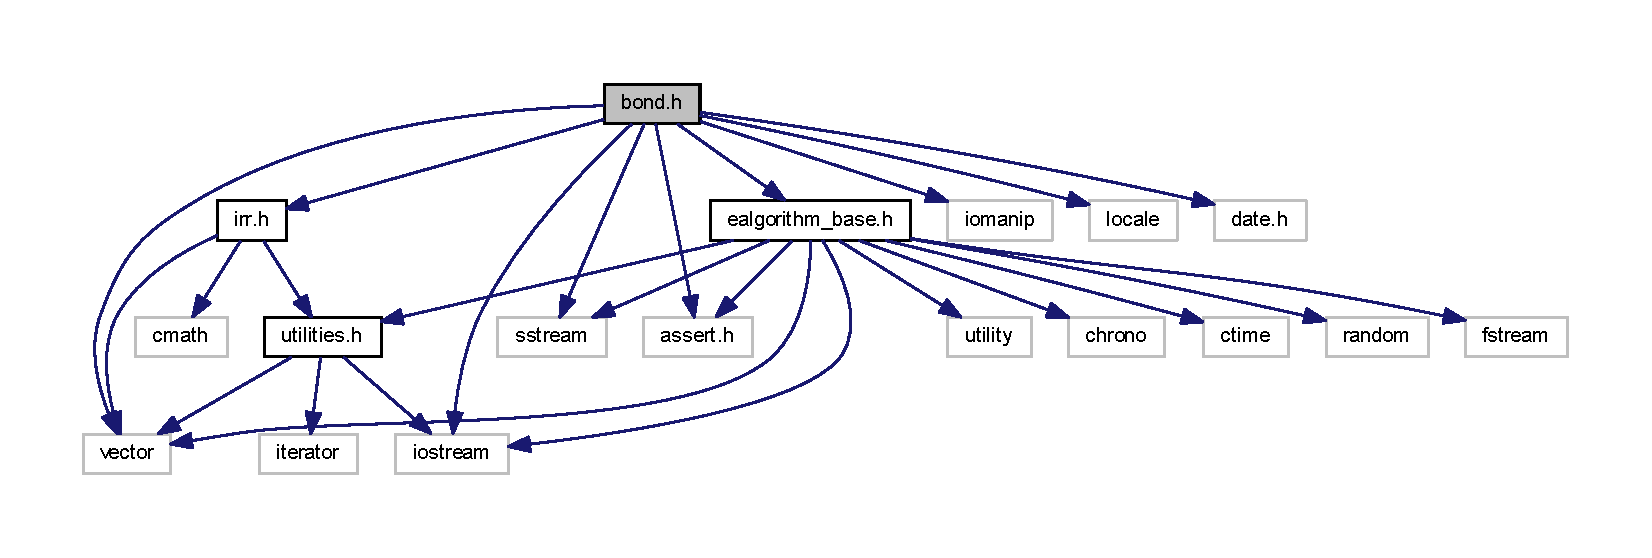
\includegraphics[width=350pt]{bond_8h__incl}
\end{center}
\end{figure}
This graph shows which files directly or indirectly include this file\+:
\nopagebreak
\begin{figure}[H]
\begin{center}
\leavevmode
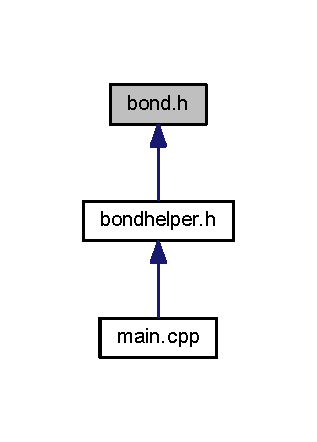
\includegraphics[width=152pt]{bond_8h__dep__incl}
\end{center}
\end{figure}
\subsection*{Classes}
\begin{DoxyCompactItemize}
\item 
class \hyperlink{classbond_1_1_bond_helper}{bond\+::\+Bond\+Helper$<$ T $>$}
\begin{DoxyCompactList}\small\item\em A class for the bond pricing problem as well as finding the yield-\/to-\/maturities of bonds. \end{DoxyCompactList}\item 
class \hyperlink{classbond_1_1_bond}{bond\+::\+Bond$<$ T $>$}
\begin{DoxyCompactList}\small\item\em \hyperlink{classbond_1_1_bond}{Bond} Class definition. \end{DoxyCompactList}\end{DoxyCompactItemize}
\subsection*{Namespaces}
\begin{DoxyCompactItemize}
\item 
 \hyperlink{namespacebond}{bond}
\begin{DoxyCompactList}\small\item\em \hyperlink{classbond_1_1_bond}{Bond} Class and Utilities. \end{DoxyCompactList}\end{DoxyCompactItemize}


\subsection{Detailed Description}
Classes and functions for bonds and their internal rate of return. 

\begin{DoxyAuthor}{Author}
Ioannis Anagnostopoulos 
\end{DoxyAuthor}

\hypertarget{bondhelper_8h}{}\section{bondhelper.\+h File Reference}
\label{bondhelper_8h}\index{bondhelper.\+h@{bondhelper.\+h}}


Classes and functions for the bond pricing problem.  


{\ttfamily \#include $<$vector$>$}\newline
{\ttfamily \#include $<$tuple$>$}\newline
{\ttfamily \#include $<$limits$>$}\newline
{\ttfamily \#include \char`\"{}bond.\+h\char`\"{}}\newline
{\ttfamily \#include \char`\"{}svensson.\+h\char`\"{}}\newline
{\ttfamily \#include \char`\"{}yield\+\_\+curve\+\_\+fitting.\+h\char`\"{}}\newline
Include dependency graph for bondhelper.\+h\+:
\nopagebreak
\begin{figure}[H]
\begin{center}
\leavevmode
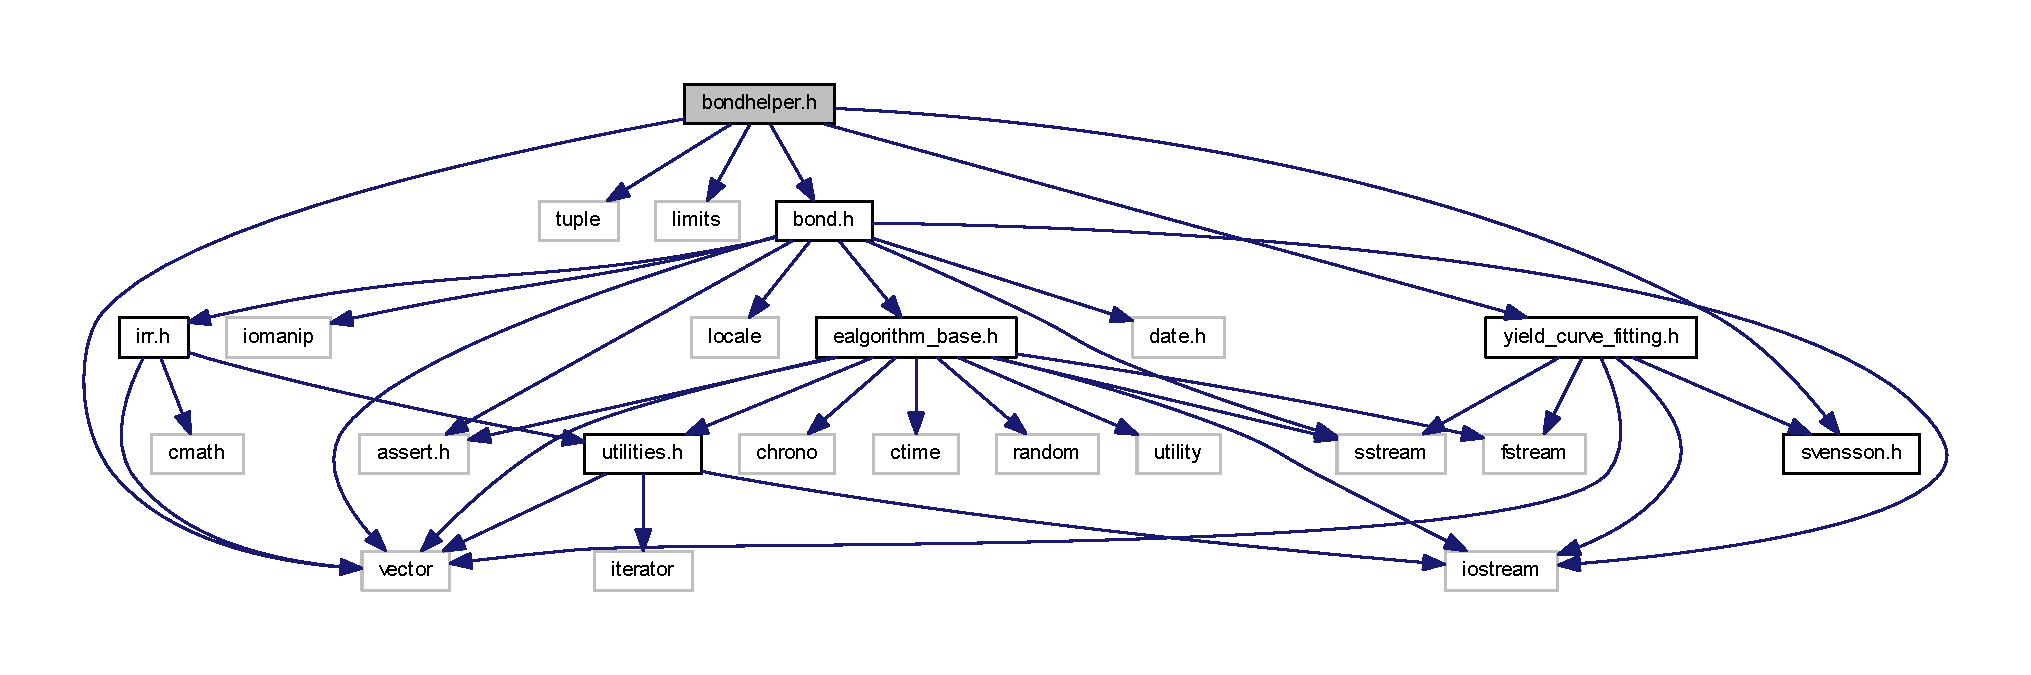
\includegraphics[width=350pt]{bondhelper_8h__incl}
\end{center}
\end{figure}
This graph shows which files directly or indirectly include this file\+:
\nopagebreak
\begin{figure}[H]
\begin{center}
\leavevmode
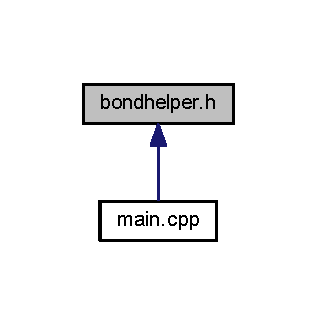
\includegraphics[width=152pt]{bondhelper_8h__dep__incl}
\end{center}
\end{figure}
\subsection*{Classes}
\begin{DoxyCompactItemize}
\item 
class \hyperlink{classbond_1_1_bond_helper}{bond\+::\+Bond\+Helper$<$ T $>$}
\begin{DoxyCompactList}\small\item\em A class for the bond pricing problem as well as finding the yield-\/to-\/maturities of bonds. \end{DoxyCompactList}\end{DoxyCompactItemize}
\subsection*{Namespaces}
\begin{DoxyCompactItemize}
\item 
 \hyperlink{namespacebond}{bond}
\begin{DoxyCompactList}\small\item\em \hyperlink{classbond_1_1_bond}{Bond} Class and Utilities. \end{DoxyCompactList}\end{DoxyCompactItemize}
\subsection*{Enumerations}
\begin{DoxyCompactItemize}
\item 
enum \hyperlink{namespacebond_a7ff8132c72465682a65a634ca0958df9}{bond\+::\+Bond\+\_\+pricing\+\_\+type} \{ \hyperlink{namespacebond_a7ff8132c72465682a65a634ca0958df9a0c68c2daa0334704116676287d54c2ae}{bond\+::\+Bond\+\_\+pricing\+\_\+type\+::bpp}, 
\hyperlink{namespacebond_a7ff8132c72465682a65a634ca0958df9afebbcc7d14e1ada7b0eee6411e82665b}{bond\+::\+Bond\+\_\+pricing\+\_\+type\+::bpy}
 \}\begin{DoxyCompactList}\small\item\em Enumeration for type of bondpricing, using yields or prices. \end{DoxyCompactList}
\end{DoxyCompactItemize}
\subsection*{Functions}
\begin{DoxyCompactItemize}
\item 
{\footnotesize template$<$typename T $>$ }\\std\+::vector$<$ Bond$<$ T $>$ $>$ \hyperlink{namespacebond_a20b23f0d31139a065334fd997507b1ae}{bond\+::read\+\_\+bonds\+\_\+from\+\_\+file} (const std\+::string \&filename)
\begin{DoxyCompactList}\small\item\em Reads bond data from a file. \end{DoxyCompactList}\end{DoxyCompactItemize}


\subsection{Detailed Description}
Classes and functions for the bond pricing problem. 

\begin{DoxyAuthor}{Author}
Ioannis Anagnostopoulos 
\end{DoxyAuthor}

\hypertarget{differentialevo_8h}{}\section{differentialevo.\+h File Reference}
\label{differentialevo_8h}\index{differentialevo.\+h@{differentialevo.\+h}}


Classes and functions for Differential Evolution.  


{\ttfamily \#include \char`\"{}ealgorithm\+\_\+base.\+h\char`\"{}}\newline
Include dependency graph for differentialevo.\+h\+:
\nopagebreak
\begin{figure}[H]
\begin{center}
\leavevmode
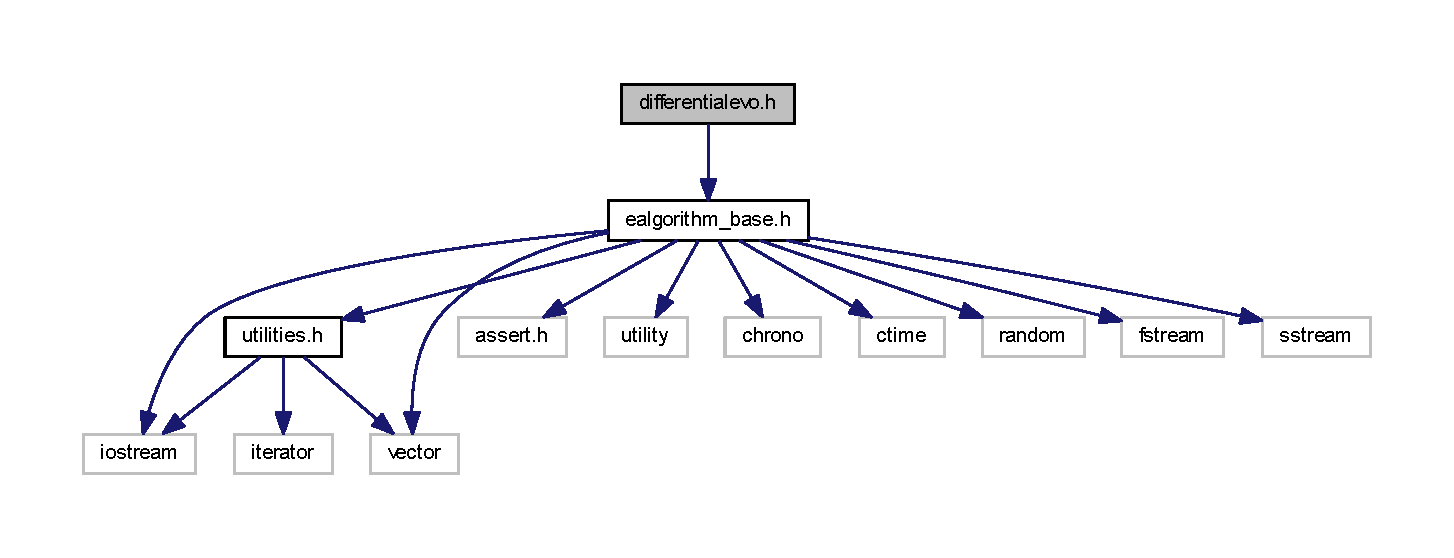
\includegraphics[width=350pt]{differentialevo_8h__incl}
\end{center}
\end{figure}
This graph shows which files directly or indirectly include this file\+:
\nopagebreak
\begin{figure}[H]
\begin{center}
\leavevmode
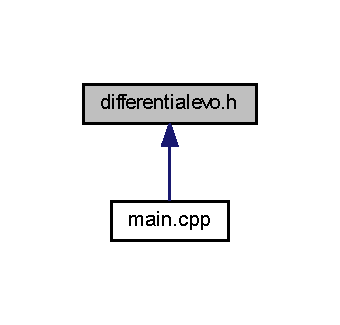
\includegraphics[width=163pt]{differentialevo_8h__dep__incl}
\end{center}
\end{figure}
\subsection*{Classes}
\begin{DoxyCompactItemize}
\item 
struct \hyperlink{structea_1_1_d_e}{ea\+::\+D\+E$<$ T $>$}
\begin{DoxyCompactList}\small\item\em Differential Evolution Structure, used in the actual algorithm and for type deduction. \end{DoxyCompactList}\item 
class \hyperlink{classea_1_1_solver_3_01_d_e_00_01_t_00_01_f_00_01_c_01_4}{ea\+::\+Solver$<$ D\+E, T, F, C $>$}
\begin{DoxyCompactList}\small\item\em Differential Evolution Algorithm (\hyperlink{structea_1_1_d_e}{DE}) Class. \end{DoxyCompactList}\end{DoxyCompactItemize}
\subsection*{Namespaces}
\begin{DoxyCompactItemize}
\item 
 \hyperlink{namespaceea}{ea}
\begin{DoxyCompactList}\small\item\em Evolutionary Algorithms. \end{DoxyCompactList}\end{DoxyCompactItemize}


\subsection{Detailed Description}
Classes and functions for Differential Evolution. 

\begin{DoxyAuthor}{Author}
Ioannis Anagnostopoulos 
\end{DoxyAuthor}

\hypertarget{ealgorithm__base_8h}{}\section{ealgorithm\+\_\+base.\+h File Reference}
\label{ealgorithm__base_8h}\index{ealgorithm\+\_\+base.\+h@{ealgorithm\+\_\+base.\+h}}


Classes and functions for the base of the solvers.  


{\ttfamily \#include $<$iostream$>$}\newline
{\ttfamily \#include $<$vector$>$}\newline
{\ttfamily \#include $<$assert.\+h$>$}\newline
{\ttfamily \#include $<$utility$>$}\newline
{\ttfamily \#include $<$chrono$>$}\newline
{\ttfamily \#include $<$ctime$>$}\newline
{\ttfamily \#include $<$random$>$}\newline
{\ttfamily \#include $<$fstream$>$}\newline
{\ttfamily \#include $<$sstream$>$}\newline
{\ttfamily \#include \char`\"{}utilities.\+h\char`\"{}}\newline
Include dependency graph for ealgorithm\+\_\+base.\+h\+:
\nopagebreak
\begin{figure}[H]
\begin{center}
\leavevmode
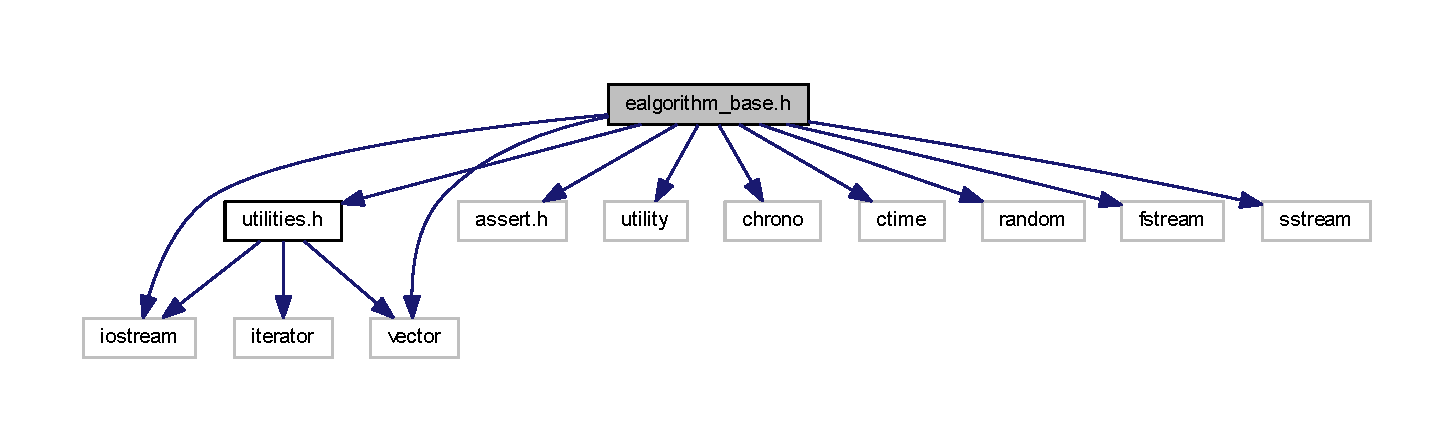
\includegraphics[width=350pt]{ealgorithm__base_8h__incl}
\end{center}
\end{figure}
This graph shows which files directly or indirectly include this file\+:
\nopagebreak
\begin{figure}[H]
\begin{center}
\leavevmode
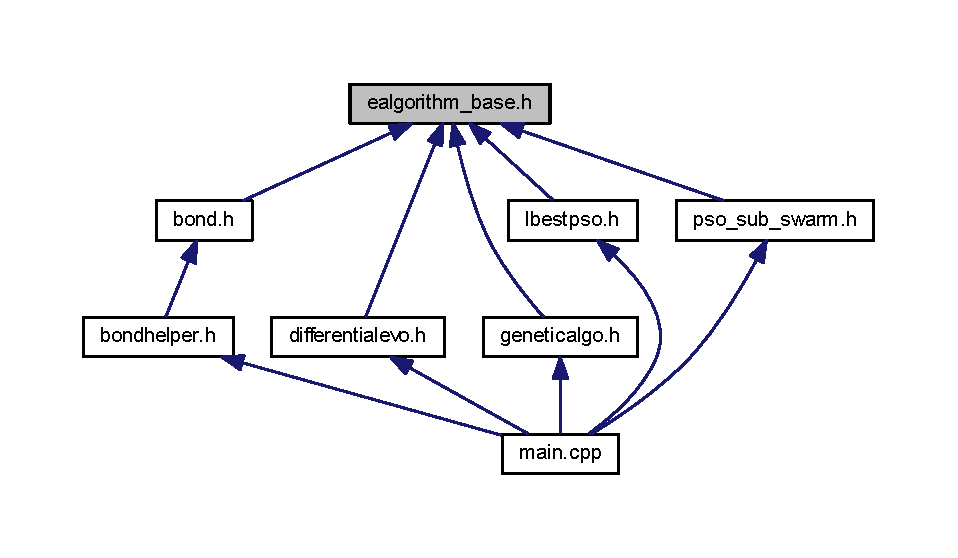
\includegraphics[width=350pt]{ealgorithm__base_8h__dep__incl}
\end{center}
\end{figure}
\subsection*{Classes}
\begin{DoxyCompactItemize}
\item 
struct \hyperlink{structea_1_1_e_a__base}{ea\+::\+E\+A\+\_\+base$<$ T $>$}
\begin{DoxyCompactList}\small\item\em Evolutionary algorithm stucture base. \end{DoxyCompactList}\item 
class \hyperlink{classea_1_1_solver}{ea\+::\+Solver$<$ S, T, F, C $>$}
\begin{DoxyCompactList}\small\item\em Template Class for Solvers. \end{DoxyCompactList}\item 
class \hyperlink{classea_1_1_solver__base}{ea\+::\+Solver\+\_\+base$<$ Derived, S, T, F, C $>$}
\begin{DoxyCompactList}\small\item\em Base Class for Evolutionary Algorithms. \end{DoxyCompactList}\end{DoxyCompactItemize}
\subsection*{Namespaces}
\begin{DoxyCompactItemize}
\item 
 \hyperlink{namespaceea}{ea}
\begin{DoxyCompactList}\small\item\em Evolutionary Algorithms. \end{DoxyCompactList}\end{DoxyCompactItemize}
\subsection*{Functions}
\begin{DoxyCompactItemize}
\item 
std\+::mt19937\+\_\+64 \hyperlink{namespaceea_a385e8ca8ba4ae2f69dcfffa79f20c2ff}{ea\+::generator} (rd())
\begin{DoxyCompactList}\small\item\em Pseudo-\/random number generator. \end{DoxyCompactList}\item 
{\footnotesize template$<$typename F , typename C , template$<$ typename $>$ class S, typename T $>$ }\\std\+::vector$<$ T $>$ \hyperlink{namespaceea_a6450b5bf61e9fdca8b6c19267e14c560}{ea\+::solve} (const F \&f, const C \&c, const S$<$ T $>$ \&solver\+\_\+struct, const std\+::string \&problem\+\_\+name)
\begin{DoxyCompactList}\small\item\em \hyperlink{classea_1_1_solver}{Solver} wrapper function, interface to solvers \+: free function used for benchmarks. \end{DoxyCompactList}\end{DoxyCompactItemize}
\subsection*{Variables}
\begin{DoxyCompactItemize}
\item 
std\+::random\+\_\+device \hyperlink{namespaceea_a0d4adcfbf42f88a74097673d4564f757}{ea\+::rd}
\begin{DoxyCompactList}\small\item\em Random device / Random number generator. \end{DoxyCompactList}\end{DoxyCompactItemize}


\subsection{Detailed Description}
Classes and functions for the base of the solvers. 

\begin{DoxyAuthor}{Author}
Ioannis Anagnostopoulos 
\end{DoxyAuthor}

\hypertarget{geneticalgo_8h}{}\section{geneticalgo.\+h File Reference}
\label{geneticalgo_8h}\index{geneticalgo.\+h@{geneticalgo.\+h}}


Classes and functions for Genetic Algorithms.  


{\ttfamily \#include \char`\"{}ealgorithm\+\_\+base.\+h\char`\"{}}\newline
{\ttfamily \#include $<$boost/math/distributions.\+hpp$>$}\newline
Include dependency graph for geneticalgo.\+h\+:
\nopagebreak
\begin{figure}[H]
\begin{center}
\leavevmode
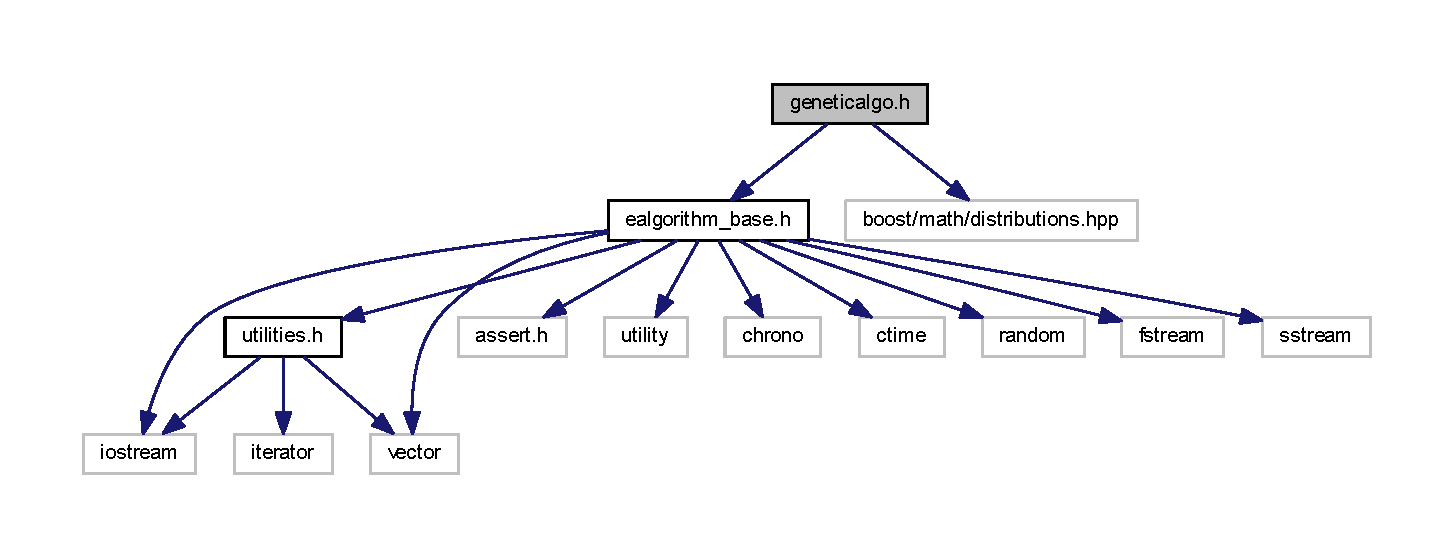
\includegraphics[width=350pt]{geneticalgo_8h__incl}
\end{center}
\end{figure}
This graph shows which files directly or indirectly include this file\+:
\nopagebreak
\begin{figure}[H]
\begin{center}
\leavevmode
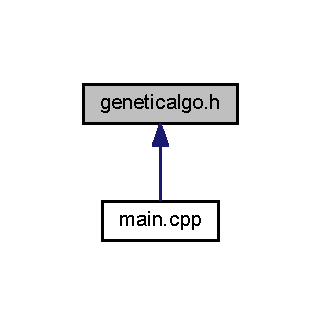
\includegraphics[width=154pt]{geneticalgo_8h__dep__incl}
\end{center}
\end{figure}
\subsection*{Classes}
\begin{DoxyCompactItemize}
\item 
struct \hyperlink{structea_1_1_g_a}{ea\+::\+G\+A$<$ T $>$}
\begin{DoxyCompactList}\small\item\em Genetic Algorithms Structure, used in the actual algorithm and for type deduction. \end{DoxyCompactList}\item 
class \hyperlink{classea_1_1_solver_3_01_g_a_00_01_t_00_01_f_00_01_c_01_4}{ea\+::\+Solver$<$ G\+A, T, F, C $>$}
\begin{DoxyCompactList}\small\item\em Genetic Algorithms (\hyperlink{structea_1_1_g_a}{GA}) Class. \end{DoxyCompactList}\end{DoxyCompactItemize}
\subsection*{Namespaces}
\begin{DoxyCompactItemize}
\item 
 \hyperlink{namespaceea}{ea}
\begin{DoxyCompactList}\small\item\em Evolutionary Algorithms. \end{DoxyCompactList}\end{DoxyCompactItemize}
\subsection*{Enumerations}
\begin{DoxyCompactItemize}
\item 
enum \hyperlink{namespaceea_a8e369877773b4db67b8512efdb4f8f89}{ea\+::\+Strategy} \{ \hyperlink{namespaceea_a8e369877773b4db67b8512efdb4f8f89ac4a301043ce8554dfced7a0c0698bdad}{ea\+::\+Strategy\+::keep\+\_\+same}, 
\hyperlink{namespaceea_a8e369877773b4db67b8512efdb4f8f89a49a303c9c8d8a0c15a7fc97cd4b1db0d}{ea\+::\+Strategy\+::re\+\_\+mutate}, 
\hyperlink{namespaceea_a8e369877773b4db67b8512efdb4f8f89a0f6969d7052da9261e31ddb6e88c136e}{ea\+::\+Strategy\+::remove}, 
\hyperlink{namespaceea_a8e369877773b4db67b8512efdb4f8f89a334c4a4c42fdb79d7ebc3e73b517e6f8}{ea\+::\+Strategy\+::none}
 \}\begin{DoxyCompactList}\small\item\em Replacing or remove individuals strategies during mutation. \end{DoxyCompactList}
\end{DoxyCompactItemize}


\subsection{Detailed Description}
Classes and functions for Genetic Algorithms. 

\begin{DoxyAuthor}{Author}
Ioannis Anagnostopoulos 
\end{DoxyAuthor}

\hypertarget{irr_8h}{}\section{irr.\+h File Reference}
\label{irr_8h}\index{irr.\+h@{irr.\+h}}


Functions for the Internal Rate of Return.  


{\ttfamily \#include $<$vector$>$}\newline
{\ttfamily \#include $<$cmath$>$}\newline
{\ttfamily \#include \char`\"{}utilities.\+h\char`\"{}}\newline
Include dependency graph for irr.\+h\+:
\nopagebreak
\begin{figure}[H]
\begin{center}
\leavevmode
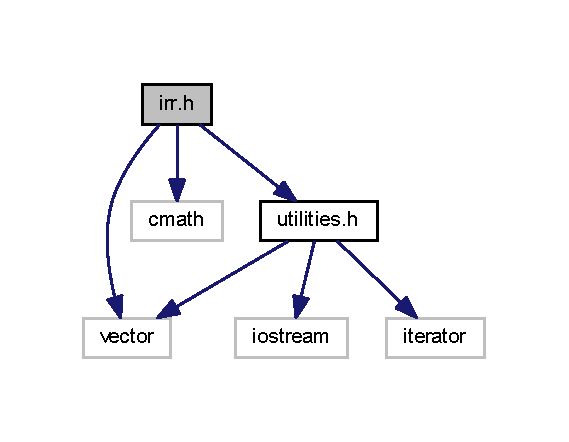
\includegraphics[width=273pt]{irr_8h__incl}
\end{center}
\end{figure}
This graph shows which files directly or indirectly include this file\+:
\nopagebreak
\begin{figure}[H]
\begin{center}
\leavevmode
\includegraphics[width=152pt]{irr_8h__dep__incl}
\end{center}
\end{figure}
\subsection*{Namespaces}
\begin{DoxyCompactItemize}
\item 
 \hyperlink{namespaceirr}{irr}
\begin{DoxyCompactList}\small\item\em Internal Rate of Return (I\+RR) namespace. \end{DoxyCompactList}\end{DoxyCompactItemize}
\subsection*{Functions}
\begin{DoxyCompactItemize}
\item 
{\footnotesize template$<$typename T $>$ }\\T \hyperlink{namespaceirr_ae00c3409ca39fa2dc47ce61da4169a66}{irr\+::compute\+\_\+discount\+\_\+factor} (const T \&r, const T \&period, const \hyperlink{namespaceutilities_ad4290e607d0651ce53db6e5c776aca7c}{D\+F\+\_\+type} \&df\+\_\+type)
\begin{DoxyCompactList}\small\item\em Calculates discount factors. \end{DoxyCompactList}\item 
{\footnotesize template$<$typename T $>$ }\\bool \hyperlink{namespaceirr_a6801aa96a307b3f52817dd1a3bcd065e}{irr\+::constraints\+\_\+irr} (const std\+::vector$<$ T $>$ \&solution, const \hyperlink{namespaceutilities_ab1a1517bf6e62a1acfab5293ca8985c1}{Constraints\+\_\+type} \&constraints\+\_\+type)
\begin{DoxyCompactList}\small\item\em Constraints function for Internal Rate of Return. \end{DoxyCompactList}\item 
{\footnotesize template$<$typename T $>$ }\\T \hyperlink{namespaceirr_ac3411cd2ad174f399c525d8d17dcdad0}{irr\+::compute\+\_\+pv} (const T \&r, const T \&nominal\+\_\+value, const std\+::vector$<$ T $>$ \&cash\+\_\+flows, const std\+::vector$<$ T $>$ \&time\+\_\+periods, const \hyperlink{namespaceutilities_ad4290e607d0651ce53db6e5c776aca7c}{D\+F\+\_\+type} \&df\+\_\+type)
\begin{DoxyCompactList}\small\item\em Returns the present value of an investment. \end{DoxyCompactList}\item 
{\footnotesize template$<$typename T $>$ }\\T \hyperlink{namespaceirr_abd1d21a84003df6b46dc32c3a30d2269}{irr\+::penalty\+\_\+irr} (const T \&r)
\begin{DoxyCompactList}\small\item\em Penalty function for I\+RR. \end{DoxyCompactList}\item 
{\footnotesize template$<$typename T $>$ }\\T \hyperlink{namespaceirr_aced01c5e5ef9e171a3b892275d442f8d}{irr\+::fitness\+\_\+irr} (const std\+::vector$<$ T $>$ \&solution, const T \&price, const T \&nominal\+\_\+value, const std\+::vector$<$ T $>$ \&cash\+\_\+flows, const std\+::vector$<$ T $>$ \&time\+\_\+periods, const \hyperlink{namespaceutilities_ad4290e607d0651ce53db6e5c776aca7c}{D\+F\+\_\+type} \&df\+\_\+type, const bool \&use\+\_\+penalty\+\_\+method)
\begin{DoxyCompactList}\small\item\em This is the fitness function for finding the internal rate of return of a bond, in this case it is equal to its yield to maturity. \end{DoxyCompactList}\end{DoxyCompactItemize}


\subsection{Detailed Description}
Functions for the Internal Rate of Return. 

\begin{DoxyAuthor}{Author}
Ioannis Anagnostopoulos 
\end{DoxyAuthor}

\hypertarget{lbestpso_8h}{}\section{lbestpso.\+h File Reference}
\label{lbestpso_8h}\index{lbestpso.\+h@{lbestpso.\+h}}


Classes and functions for the lbest (Local Best) Particle Swarm Optimisation with a ring topology.  


{\ttfamily \#include $<$unordered\+\_\+map$>$}\newline
{\ttfamily \#include $<$boost/math/constants/constants.\+hpp$>$}\newline
{\ttfamily \#include \char`\"{}ealgorithm\+\_\+base.\+h\char`\"{}}\newline
{\ttfamily \#include $<$array$>$}\newline
Include dependency graph for lbestpso.\+h\+:
\nopagebreak
\begin{figure}[H]
\begin{center}
\leavevmode
\includegraphics[width=350pt]{lbestpso_8h__incl}
\end{center}
\end{figure}
This graph shows which files directly or indirectly include this file\+:
\nopagebreak
\begin{figure}[H]
\begin{center}
\leavevmode
\includegraphics[width=142pt]{lbestpso_8h__dep__incl}
\end{center}
\end{figure}
\subsection*{Classes}
\begin{DoxyCompactItemize}
\item 
struct \hyperlink{structea_1_1_p_s_ol}{ea\+::\+P\+S\+Ol$<$ T $>$}
\begin{DoxyCompactList}\small\item\em Local Best Particle Swarm Optimisation Structure, used in the actual algorithm and for type deduction. \end{DoxyCompactList}\item 
class \hyperlink{classea_1_1_solver_3_01_p_s_ol_00_01_t_00_01_f_00_01_c_01_4}{ea\+::\+Solver$<$ P\+S\+Ol, T, F, C $>$}
\begin{DoxyCompactList}\small\item\em Local Best Particle Swarm Optimisation (P\+SO) Class. \end{DoxyCompactList}\end{DoxyCompactItemize}
\subsection*{Namespaces}
\begin{DoxyCompactItemize}
\item 
 \hyperlink{namespaceea}{ea}
\begin{DoxyCompactList}\small\item\em Evolutionary Algorithms. \end{DoxyCompactList}\end{DoxyCompactItemize}
\subsection*{Variables}
\begin{DoxyCompactItemize}
\item 
{\footnotesize template$<$typename T $>$ }\\const double \hyperlink{namespaceea_a0a68157259a48341f23eeffca8a1d748}{ea\+::inv\+\_\+pi\+\_\+sq} = 1 / std\+::pow(boost\+::math\+::constants\+::pi$<$T$>$(), 2)
\begin{DoxyCompactList}\small\item\em Inverse square of pi constant. \end{DoxyCompactList}\end{DoxyCompactItemize}


\subsection{Detailed Description}
Classes and functions for the lbest (Local Best) Particle Swarm Optimisation with a ring topology. 

\begin{DoxyAuthor}{Author}
Ioannis Anagnostopoulos 
\end{DoxyAuthor}

\hypertarget{main_8cpp}{}\section{main.\+cpp File Reference}
\label{main_8cpp}\index{main.\+cpp@{main.\+cpp}}


A showcase of the application of the solvers on the Yield Curve Fitting, Internal Rate of Return Estimation and Bond Pricing Problems.  


{\ttfamily \#include \char`\"{}../src/bondhelper.\+h\char`\"{}}\newline
{\ttfamily \#include \char`\"{}../src/geneticalgo.\+h\char`\"{}}\newline
{\ttfamily \#include \char`\"{}../src/pso\+\_\+sub\+\_\+swarm.\+h\char`\"{}}\newline
{\ttfamily \#include \char`\"{}../src/differentialevo.\+h\char`\"{}}\newline
{\ttfamily \#include \char`\"{}../src/lbestpso.\+h\char`\"{}}\newline
Include dependency graph for main.\+cpp\+:
\nopagebreak
\begin{figure}[H]
\begin{center}
\leavevmode
\includegraphics[width=350pt]{main_8cpp__incl}
\end{center}
\end{figure}
\subsection*{Functions}
\begin{DoxyCompactItemize}
\item 
int \hyperlink{main_8cpp_ae66f6b31b5ad750f1fe042a706a4e3d4}{main} ()
\end{DoxyCompactItemize}


\subsection{Detailed Description}
A showcase of the application of the solvers on the Yield Curve Fitting, Internal Rate of Return Estimation and Bond Pricing Problems. 

\begin{DoxyAuthor}{Author}
Ioannis Anagnostopoulos
\end{DoxyAuthor}
Usage is the following\+:

Step 1\+:Create a solver structure object \{GA, DE, P\+S\+Ol\} with a specific floating-\/point number type, setting all of its parameters throught its constructor.

Set print\+\_\+to\+\_\+output or print\+\_\+to\+\_\+display to false if there is no need for displaying the results to terminal or printing them to a file.

Step 2\+: Either use the common interface solve solve(const F\& f, const C\& c, const S$<$\+T$>$\& solver\+\_\+struct, const std\+::string\& problem\+\_\+name) passing the objective and constraint functions as lambda functions (anonymous functions) capturing all the required variables, such as bonds or use the public interfaces from the Interest\+\_\+\+Rate\+\_\+\+Helper (Yield Curve Fitting), Bond\+Helper (Internal Rate of Return estimation and bond pricing for a number of bonds) and Bond (Internal Rate of Return Estimation and Macaulay Duration Estimation) classes after creating an object instance of those classes using their constructors. 

\subsection{Function Documentation}
\mbox{\Hypertarget{main_8cpp_ae66f6b31b5ad750f1fe042a706a4e3d4}\label{main_8cpp_ae66f6b31b5ad750f1fe042a706a4e3d4}} 
\index{main.\+cpp@{main.\+cpp}!main@{main}}
\index{main@{main}!main.\+cpp@{main.\+cpp}}
\subsubsection{\texorpdfstring{main()}{main()}}
{\footnotesize\ttfamily int main (\begin{DoxyParamCaption}{ }\end{DoxyParamCaption})}

Call benchmark functions

I\+RR solvers 

Definition at line 75 of file main.\+cpp.


\begin{DoxyCode}
76 \{
77     \textcolor{keyword}{using namespace }\hyperlink{namespaceyft}{yft};
78     \textcolor{keyword}{using namespace }\hyperlink{namespacebond}{bond};
79     \textcolor{keyword}{const} std::vector<double> stdev \{ 0.7, 0.7, 0.7, 0.7, 0.7, 0.7 \};
80     \textcolor{keyword}{const} std::vector<double> stdev\_ga\{ 0.5, 0.5, 0.5, 0.5, 0.5, 0.5 \};
81     \textcolor{keywordtype}{double} irr\_tol = 0.00000001;
82     \textcolor{keywordtype}{double} tol = 0.0001;
83     \textcolor{keywordtype}{double} tol\_f = 0.001;
85     \hyperlink{classyft_1_1_interest___rate___helper}{Interest\_Rate\_Helper<double>} ir\{ read\_ir\_from\_file<double>(\textcolor{stringliteral}{"
      interest\_rate\_data\_periods.txt"}) \};
86     \hyperlink{classbond_1_1_bond_helper}{BondHelper<double>} de\{ read\_bonds\_from\_file<double>(\textcolor{stringliteral}{"bond\_data.txt"}), DF\_type::exp \};
88     \hyperlink{structea_1_1_d_e}{DE<double>} de\_irr\{ 1, 0.6,\{ 0.05 \},\{ 0.7 \}, 10, irr\_tol, 500, \textcolor{keyword}{false}, Constraints\_type::normal
      , \textcolor{keyword}{true}, \textcolor{keyword}{true} \};
89     \hyperlink{structea_1_1_d_e}{DE<double>} de\_irr\_check\{ 1, 0.6,\{ 0.05 \},\{ 0.7 \}, 10, irr\_tol, 500, \textcolor{keyword}{false}, 
      Constraints\_type::normal, \textcolor{keyword}{false}, \textcolor{keyword}{false} \};
90     GA<double> ga\_irr\{ 0.4, 0.35, 6.0, \{ 0.05 \},\{ 0.5 \}, 42, irr\_tol, 2000, \textcolor{keyword}{false}, Constraints\_type::normal
      , Strategy::remove, \textcolor{keyword}{true}, \textcolor{keyword}{true}\};
91     PSOl<double> pso\_irr\{ 1.49618, 0.9, \{ 1000000 \},\{ 0.05 \},\{ 0.7 \}, 22, irr\_tol, 3000, \textcolor{keyword}{false}, 
      Constraints\_type::normal, \textcolor{keyword}{true}, \textcolor{keyword}{true}\};
92     \textcolor{keyword}{auto} decision\_variables = de.set\_init\_nss\_params(de\_irr);
93     \hyperlink{structea_1_1_d_e}{DE<double>} de\_pricing\{ 1, 0.6, decision\_variables, stdev, 60, tol, 500, \textcolor{keyword}{false}, 
      Constraints\_type::tight, \textcolor{keyword}{true}, \textcolor{keyword}{true} \};
94     \hyperlink{structea_1_1_d_e}{DE<double>} de\_fitting\{ 1, 0.6, decision\_variables, stdev, 60, tol\_f, 500, \textcolor{keyword}{false}, 
      Constraints\_type::tight, \textcolor{keyword}{true}, \textcolor{keyword}{true} \};
95     GA<double> ga\_pricing\{ 0.4, 0.35, 6.0, decision\_variables, stdev\_ga, 250, tol, 2000, \textcolor{keyword}{false}, 
      Constraints\_type::tight, Strategy::remove, \textcolor{keyword}{true}, \textcolor{keyword}{true} \};
96     GA<double> ga\_fitting\{ 0.4, 0.35, 6.0, decision\_variables, stdev\_ga, 250, tol\_f, 2000, \textcolor{keyword}{false}, 
      Constraints\_type::tight, Strategy::remove, \textcolor{keyword}{true}, \textcolor{keyword}{true} \};
97     PSOl<double> pso\_pricing\{ 1.49618, 0.9, \{ 100000, 100000, 100000, 100000, 100000, 100000 \}, 
      decision\_variables, stdev, 130, tol, 3000, \textcolor{keyword}{false}, Constraints\_type::tight, \textcolor{keyword}{true}, \textcolor{keyword}{true} \};
98     PSOl<double> pso\_fitting\{ 1.49618, 0.9, \{ 100000, 100000, 100000, 100000, 100000, 100000 \}, 
      decision\_variables, stdev, 130, tol\_f, 3000, \textcolor{keyword}{false}, Constraints\_type::tight, \textcolor{keyword}{true}, \textcolor{keyword}{true} \};
99     PSOs<double> pso\_pricing\{ 2.05, 2.05, 6, 0.9, 1.0,\{ 100000, 100000, 100000, 100000, 100000, 100000 \}, 
      decision\_variables, stdev, 24, tol, 1000, \textcolor{keyword}{false}, Constraints\_type::none, \textcolor{keyword}{true}, \textcolor{keyword}{true} \};
100     \textcolor{keywordflow}{for} (\textcolor{keywordtype}{size\_t} i = 0; i < 100; ++i)
101     \{
102         de.bond\_pricing(ga\_pricing, de\_irr\_check, Bond\_pricing\_type::bpp);
103         ir.yieldcurve\_fitting(ga\_fitting);
104         de.bond\_pricing(de\_pricing, de\_irr\_check, Bond\_pricing\_type::bpp);
105         ir.yieldcurve\_fitting(de\_fitting);
106         de.bond\_pricing(pso\_pricing, de\_irr\_check, Bond\_pricing\_type::bpp);
107         ir.yieldcurve\_fitting(pso\_fitting);
108         de.set\_init\_nss\_params(de\_irr);
109         de.set\_init\_nss\_params(pso\_irr);
110         de.set\_init\_nss\_params(ga\_irr);
111     \}
112     \textcolor{keywordflow}{return} 0;
113 \}
\end{DoxyCode}

\hypertarget{pso__sub__swarm_8h}{}\section{pso\+\_\+sub\+\_\+swarm.\+h File Reference}
\label{pso__sub__swarm_8h}\index{pso\+\_\+sub\+\_\+swarm.\+h@{pso\+\_\+sub\+\_\+swarm.\+h}}


Classes and functions for the initial implementation of Sub-\/\+Swarm Particle Swarm Optimisation.  


{\ttfamily \#include \char`\"{}ealgorithm\+\_\+base.\+h\char`\"{}}\newline
{\ttfamily \#include $<$unordered\+\_\+map$>$}\newline
Include dependency graph for pso\+\_\+sub\+\_\+swarm.\+h\+:
\nopagebreak
\begin{figure}[H]
\begin{center}
\leavevmode
\includegraphics[width=350pt]{pso__sub__swarm_8h__incl}
\end{center}
\end{figure}
This graph shows which files directly or indirectly include this file\+:
\nopagebreak
\begin{figure}[H]
\begin{center}
\leavevmode
\includegraphics[width=175pt]{pso__sub__swarm_8h__dep__incl}
\end{center}
\end{figure}
\subsection*{Classes}
\begin{DoxyCompactItemize}
\item 
struct \hyperlink{structea_1_1_p_s_os}{ea\+::\+P\+S\+Os$<$ T $>$}
\begin{DoxyCompactList}\small\item\em Particle Swarm Optimisation Structure, used in the actual algorithm and for type deduction. \end{DoxyCompactList}\item 
class \hyperlink{classea_1_1_solver_3_01_p_s_os_00_01_t_00_01_f_00_01_c_01_4}{ea\+::\+Solver$<$ P\+S\+Os, T, F, C $>$}
\begin{DoxyCompactList}\small\item\em Sub-\/\+Swarm Particle Swarm Optimisation (P\+SO) Class. \end{DoxyCompactList}\end{DoxyCompactItemize}
\subsection*{Namespaces}
\begin{DoxyCompactItemize}
\item 
 \hyperlink{namespaceea}{ea}
\begin{DoxyCompactList}\small\item\em Evolutionary Algorithms. \end{DoxyCompactList}\end{DoxyCompactItemize}
\subsection*{Variables}
\begin{DoxyCompactItemize}
\item 
{\footnotesize template$<$typename T $>$ }\\const double \hyperlink{namespaceea_aceb1a704bbda5c44541cd98184c2c224}{ea\+::inv\+\_\+pi\+\_\+sq\+\_\+2} = 1 / std\+::pow(boost\+::math\+::constants\+::pi$<$T$>$(), 2)
\begin{DoxyCompactList}\small\item\em Inverse square of pi constant. \end{DoxyCompactList}\end{DoxyCompactItemize}


\subsection{Detailed Description}
Classes and functions for the initial implementation of Sub-\/\+Swarm Particle Swarm Optimisation. 

\begin{DoxyAuthor}{Author}
Ioannis Anagnostopoulos 
\end{DoxyAuthor}

\hypertarget{svensson_8h}{}\section{svensson.\+h File Reference}
\label{svensson_8h}\index{svensson.\+h@{svensson.\+h}}


Functions for the Nelson-\/\+Siegel-\/\+Svensson model.  


This graph shows which files directly or indirectly include this file\+:
\nopagebreak
\begin{figure}[H]
\begin{center}
\leavevmode
\includegraphics[width=207pt]{svensson_8h__dep__incl}
\end{center}
\end{figure}
\subsection*{Namespaces}
\begin{DoxyCompactItemize}
\item 
 \hyperlink{namespacenss}{nss}
\begin{DoxyCompactList}\small\item\em Nelson-\/\+Siegel-\/\+Svensson (N\+SS) model namespace. \end{DoxyCompactList}\end{DoxyCompactItemize}
\subsection*{Functions}
\begin{DoxyCompactItemize}
\item 
{\footnotesize template$<$typename T $>$ }\\bool \hyperlink{namespacenss_a39de3569a71e773f9da82c713eb7e6eb}{nss\+::constraints\+\_\+svensson} (const std\+::vector$<$ T $>$ \&solution, const Constraints\+\_\+type \&constraints\+\_\+type)
\begin{DoxyCompactList}\small\item\em Constraints function for the N\+SS model. \end{DoxyCompactList}\item 
{\footnotesize template$<$typename T $>$ }\\T \hyperlink{namespacenss_a71aad246261afa16f8bb1a4057570d4b}{nss\+::svensson} (const std\+::vector$<$ T $>$ \&solution, const T \&m)
\begin{DoxyCompactList}\small\item\em Spot interest rate at term m using the N\+SS model. \end{DoxyCompactList}\item 
{\footnotesize template$<$typename T $>$ }\\T \hyperlink{namespacenss_a009a0ebbca20f7969d0c2ed5a241aa82}{nss\+::penalty\+\_\+svensson} (const std\+::vector$<$ T $>$ \&solution)
\begin{DoxyCompactList}\small\item\em Penalty function for N\+SS. \end{DoxyCompactList}\end{DoxyCompactItemize}


\subsection{Detailed Description}
Functions for the Nelson-\/\+Siegel-\/\+Svensson model. 

\begin{DoxyAuthor}{Author}
Ioannis Anagnostopoulos 
\end{DoxyAuthor}

\hypertarget{utilities_8h}{}\section{utilities.\+h File Reference}
\label{utilities_8h}\index{utilities.\+h@{utilities.\+h}}


Enumerations and functions used from the rest of the project.  


{\ttfamily \#include $<$iostream$>$}\newline
{\ttfamily \#include $<$vector$>$}\newline
{\ttfamily \#include $<$iterator$>$}\newline
Include dependency graph for utilities.\+h\+:
\nopagebreak
\begin{figure}[H]
\begin{center}
\leavevmode
\includegraphics[width=260pt]{utilities_8h__incl}
\end{center}
\end{figure}
This graph shows which files directly or indirectly include this file\+:
\nopagebreak
\begin{figure}[H]
\begin{center}
\leavevmode
\includegraphics[width=350pt]{utilities_8h__dep__incl}
\end{center}
\end{figure}
\subsection*{Namespaces}
\begin{DoxyCompactItemize}
\item 
 \hyperlink{namespaceutilities}{utilities}
\begin{DoxyCompactList}\small\item\em Utilities namespace. \end{DoxyCompactList}\end{DoxyCompactItemize}
\subsection*{Enumerations}
\begin{DoxyCompactItemize}
\item 
enum \hyperlink{namespaceutilities_ad4290e607d0651ce53db6e5c776aca7c}{utilities\+::\+D\+F\+\_\+type} \{ \hyperlink{namespaceutilities_ad4290e607d0651ce53db6e5c776aca7ca8a3baba97ec51277ed8ac64e456f6027}{utilities\+::\+D\+F\+\_\+type\+::frac}, 
\hyperlink{namespaceutilities_ad4290e607d0651ce53db6e5c776aca7cab0ab0254bd58eb87eaee3172ba49fefb}{utilities\+::\+D\+F\+\_\+type\+::exp}
 \}\begin{DoxyCompactList}\small\item\em Enumeration for discount factor types/methods. \end{DoxyCompactList}
\item 
enum \hyperlink{namespaceutilities_ab1a1517bf6e62a1acfab5293ca8985c1}{utilities\+::\+Constraints\+\_\+type} \{ \hyperlink{namespaceutilities_ab1a1517bf6e62a1acfab5293ca8985c1afea087517c26fadd409bd4b9dc642555}{utilities\+::\+Constraints\+\_\+type\+::normal}, 
\hyperlink{namespaceutilities_ab1a1517bf6e62a1acfab5293ca8985c1a0423fa423baf1ea8139f6662869faf2f}{utilities\+::\+Constraints\+\_\+type\+::tight}, 
\hyperlink{namespaceutilities_ab1a1517bf6e62a1acfab5293ca8985c1a334c4a4c42fdb79d7ebc3e73b517e6f8}{utilities\+::\+Constraints\+\_\+type\+::none}
 \}\begin{DoxyCompactList}\small\item\em Enumeration for types of constraints for the optimisation problems. \end{DoxyCompactList}
\end{DoxyCompactItemize}
\subsection*{Functions}
\begin{DoxyCompactItemize}
\item 
{\footnotesize template$<$typename T $>$ }\\std\+::ostream \& \hyperlink{namespaceutilities_a4b168c00efe29cabc5846b48225a6e52}{utilities\+::operator$<$$<$} (std\+::ostream \&stream, const std\+::vector$<$ T $>$ \&vector)
\begin{DoxyCompactList}\small\item\em Overload the operator $<$$<$ for printing vectors. \end{DoxyCompactList}\end{DoxyCompactItemize}


\subsection{Detailed Description}
Enumerations and functions used from the rest of the project. 

\begin{DoxyAuthor}{Author}
Ioannis Anagnostopoulos 
\end{DoxyAuthor}

\hypertarget{yield__curve__fitting_8h}{}\section{yield\+\_\+curve\+\_\+fitting.\+h File Reference}
\label{yield__curve__fitting_8h}\index{yield\+\_\+curve\+\_\+fitting.\+h@{yield\+\_\+curve\+\_\+fitting.\+h}}


Class and functions for the yield curve fitting problem.  


{\ttfamily \#include $<$iostream$>$}\newline
{\ttfamily \#include $<$fstream$>$}\newline
{\ttfamily \#include $<$sstream$>$}\newline
{\ttfamily \#include $<$vector$>$}\newline
{\ttfamily \#include \char`\"{}svensson.\+h\char`\"{}}\newline
Include dependency graph for yield\+\_\+curve\+\_\+fitting.\+h\+:
\nopagebreak
\begin{figure}[H]
\begin{center}
\leavevmode
\includegraphics[width=350pt]{yield__curve__fitting_8h__incl}
\end{center}
\end{figure}
This graph shows which files directly or indirectly include this file\+:
\nopagebreak
\begin{figure}[H]
\begin{center}
\leavevmode
\includegraphics[width=181pt]{yield__curve__fitting_8h__dep__incl}
\end{center}
\end{figure}
\subsection*{Classes}
\begin{DoxyCompactItemize}
\item 
struct \hyperlink{structyft_1_1_interest___rate}{yft\+::\+Interest\+\_\+\+Rate$<$ T $>$}
\begin{DoxyCompactList}\small\item\em Structure for interest rates. \end{DoxyCompactList}\item 
class \hyperlink{classyft_1_1_interest___rate___helper}{yft\+::\+Interest\+\_\+\+Rate\+\_\+\+Helper$<$ T $>$}
\begin{DoxyCompactList}\small\item\em A class for the yield-\/curve-\/fitting problem. \end{DoxyCompactList}\end{DoxyCompactItemize}
\subsection*{Namespaces}
\begin{DoxyCompactItemize}
\item 
 \hyperlink{namespaceyft}{yft}
\begin{DoxyCompactList}\small\item\em Yield Curve Fitting namespace. \end{DoxyCompactList}\end{DoxyCompactItemize}
\subsection*{Functions}
\begin{DoxyCompactItemize}
\item 
{\footnotesize template$<$typename T $>$ }\\std\+::vector$<$ Interest\+\_\+\+Rate$<$ T $>$ $>$ \hyperlink{namespaceyft_a5e004e321696f199f8cf25b1dc604108}{yft\+::read\+\_\+ir\+\_\+from\+\_\+file} (const std\+::string \&filename)
\begin{DoxyCompactList}\small\item\em Reads the interest rates and periods from file and constructs a vector of interest rate structs. \end{DoxyCompactList}\end{DoxyCompactItemize}


\subsection{Detailed Description}
Class and functions for the yield curve fitting problem. 

\begin{DoxyAuthor}{Author}
Ioannis Anagnostopoulos 
\end{DoxyAuthor}

%--- End generated contents ---

% Index
\backmatter
\newpage
\phantomsection
\clearemptydoublepage
\addcontentsline{toc}{chapter}{Index}
\printindex

\end{document}
